\documentclass[11pt,oneside]{book}
\usepackage{fontspec}
\setmainfont{Noto Serif}
\setsansfont{Noto Sans}
\setmonofont{Noto Sans Mono}
\newfontfamily\proseunicodefont{DejaVu Serif}
\usepackage[margin=1in]{geometry}
\usepackage{microtype}
\usepackage{amsmath,amssymb,amsthm,mathtools,bm}
\usepackage{graphicx}
\usepackage{xcolor}
\usepackage{booktabs}
\usepackage{array}
\usepackage{longtable}
\usepackage{enumitem}
\usepackage{float}
\usepackage{caption}
\usepackage{hyperref}
\usepackage{fancyhdr}
\usepackage{tikz}
\usetikzlibrary{arrows.meta,positioning,calc,decorations.pathmorphing}

\hypersetup{
  colorlinks=true,
  linkcolor=blue!50!black,
  urlcolor=blue!50!black,
  citecolor=blue!50!black
}

\setlength{\parskip}{0.5em}
\setlength{\parindent}{0pt}
\setlist[itemize]{topsep=0.25em,itemsep=0.2em}
\setlist[enumerate]{topsep=0.25em,itemsep=0.2em}
\setlength{\headheight}{40pt}
\numberwithin{equation}{chapter}

\newtheorem{theorem}{Théorème}[chapter]
\newtheorem{proposition}[theorem]{Proposition}
\newtheorem{lemma}[theorem]{Lemme}
\newtheorem{corollary}[theorem]{Corollaire}
\theoremstyle{definition}
\newtheorem{definition}[theorem]{Définition}
\newtheorem{example}[theorem]{Exemple}
\theoremstyle{remark}
\newtheorem{remark}[theorem]{Remarque}

\providecommand{\ket}[1]{\left\lvert#1\right\rangle}
\providecommand{\bra}[1]{\left\langle#1\right\rvert}
\providecommand{\braket}[2]{\left\langle#1\,\middle|\,#2\right\rangle}
\providecommand{\expect}[1]{\left\langle#1\right\rangle}
\newcommand{\lectureoverview}[1]{\paragraph{Vue d’ensemble.} #1}
\newenvironment{classroomqa}{%
  \par\medskip
  \begin{minipage}{0.96\textwidth}
}{%
  \end{minipage}
  \par\medskip
}
\newcommand{\audiencequestion}[1]{\noindent\textbf{Question du public.} #1\par\smallskip}
\newcommand{\lecturerresponse}[1]{\noindent\textbf{Réponse.} #1\par}
\newcommand{\lecturetimestamp}[1]{\footnote{Horodatage du cours : #1.}}
\newcommand{\lectureframe}[1]{\par\smallskip{\centering\footnotesize\itshape Image du cours : #1.\par}}
\newcommand{\editorialnote}[1]{\footnote{Précision éditoriale : #1}}

\makeatletter
\newcommand{\course@headerfont}{\normalfont\small\itshape}
\newcommand{\course@pagefont}{\normalfont\small}
\newcommand{\course@headerraise}{14pt}
\newlength{\course@headerboxheight}
\setlength{\course@headerboxheight}{\dimexpr\headheight-\course@headerraise-9pt\relax}
\newcommand{\course@leftheadbox}[1]{%
  \raisebox{\course@headerraise}{%
    \parbox[t][\course@headerboxheight][t]{0.82\textwidth}{%
      \raggedright\course@headerfont\strut\MakeUppercase{#1}\strut%
    }%
  }%
}
\newcommand{\course@rightheadbox}[1]{%
  \raisebox{\course@headerraise}{%
    \parbox[t][\course@headerboxheight][t]{0.82\textwidth}{%
      \raggedleft\course@headerfont\strut\MakeUppercase{#1}\strut%
    }%
  }%
}
\renewcommand{\chaptermark}[1]{\markboth{\MakeUppercase{\chaptername\ \thechapter.\ #1}}{}}
\renewcommand{\sectionmark}[1]{\markright{\MakeUppercase{\thesection\hspace{0.4em}#1}}}
\fancyhf{}
\fancyhead[L]{\course@leftheadbox{\leftmark}}
\fancyhead[R]{\course@pagefont\thepage}
\renewcommand{\headrulewidth}{0.5pt}
\pagestyle{fancy}
\fancypagestyle{plain}{%
  \fancyhf{}
  \fancyhead[L]{\course@leftheadbox{\leftmark}}
  \fancyhead[R]{\course@pagefont\thepage}
  \renewcommand{\headrulewidth}{0.5pt}
}
\makeatother

\usepackage{polyglossia}
\setdefaultlanguage{french}
\usepackage{sectsty}
\renewcommand{\contentsname}{Table des matières}
\renewcommand{\chaptername}{Chapitre}
\renewcommand{\figurename}{Figure}
\renewcommand{\tablename}{Tableau}
\renewcommand{\proofname}{Démonstration}
\renewcommand{\bibname}{Références}
\sectionfont{\raggedright}
\subsectionfont{\raggedright}
\makeatletter
\renewcommand{\@pnumwidth}{2.2em}
\renewcommand{\@tocrmarg}{3.2em}
\makeatother
\usepackage{tocloft}
\renewcommand{\cftchapfont}{\small\bfseries}
\renewcommand{\cftchappagefont}{\small\bfseries}
\renewcommand{\cftsecfont}{\small}
\renewcommand{\cftsecpagefont}{\small}
\setlength{\cftsecnumwidth}{3em}
\emergencystretch=6em
\pdfstringdefDisableCommands{\def\proseunicodefont{}}

\geometry{paperwidth=177.6mm,paperheight=252mm,left=16mm,right=16mm,
 top=18mm,bottom=18mm,includeheadfoot,headheight=28pt,headsep=7mm,footskip=9mm}
\usepackage{scrextend}
\changefontsizes[17pt]{12pt}
\raggedbottom
\renewenvironment{classroomqa}{\par\medskip\begingroup}{\par\endgroup\medskip}
\fancyhf{}
\setlength{\headwidth}{\textwidth}
\fancyhead[L]{\parbox{\textwidth}{\raggedright\fontsize{9}{11}\selectfont\nouppercase{\leftmark}}}
\fancyfoot[C]{\small\thepage}
\renewcommand{\headrulewidth}{0.3pt}
\fancypagestyle{plain}{\fancyhf{}\fancyfoot[C]{\small\thepage}\renewcommand{\headrulewidth}{0pt}}

\graphicspath{{../../../generated_course_notes/core/general_relativity/2012_fall_theoretical_minimum/figures/}{../../../generated_course_notes/core/general_relativity/2012_fall_theoretical_minimum/assets/}}
\begin{document}
\frontmatter
\hypersetup{pageanchor=false}
\begin{titlepage}
\thispagestyle{empty}
\begin{tikzpicture}[remember picture,overlay]
  \node[anchor=center,inner sep=0] at (current page.center) {%
    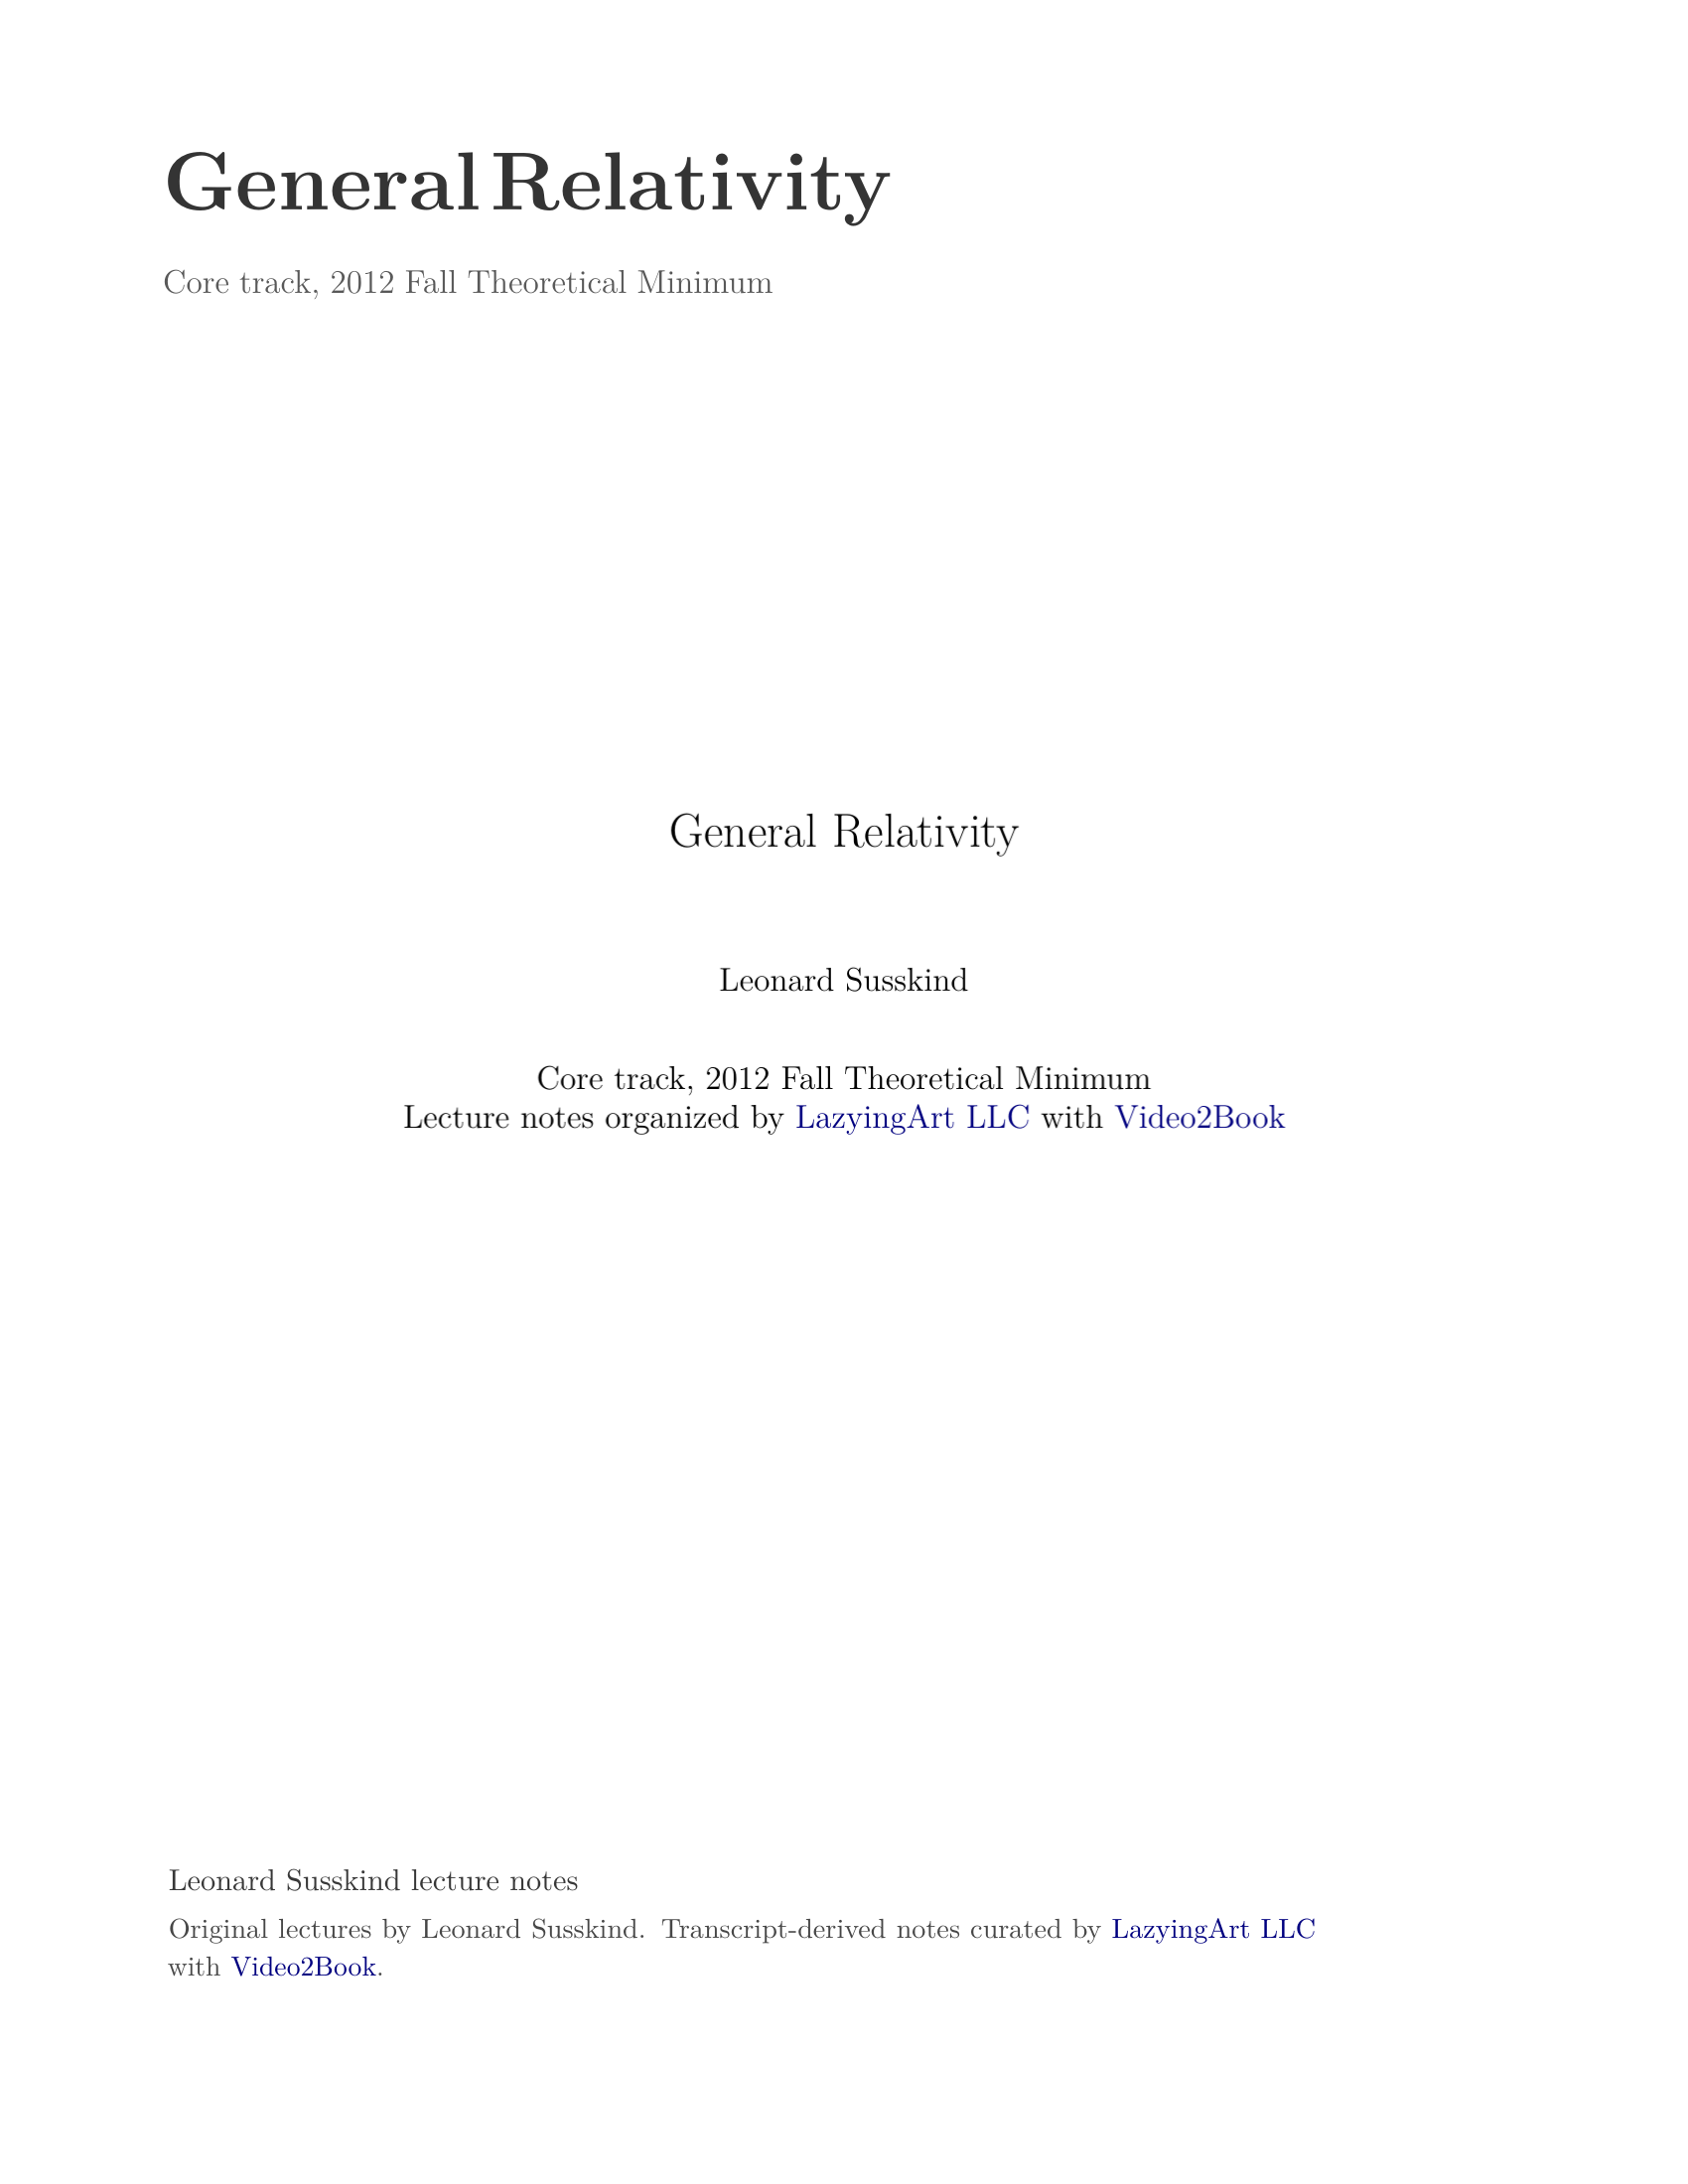
\includegraphics[height=\paperheight,keepaspectratio]{../../../generated_course_notes/core/general_relativity/2012_fall_theoretical_minimum/assets/cover-art.png}%
  };
  \node[
    anchor=north west,
    align=left,
    text width=0.78\paperwidth,
    fill=white,
    fill opacity=0.9,
    rounded corners=8pt,
    inner xsep=10pt,
    inner ysep=8pt
  ] at ([xshift=0.08\paperwidth,yshift=-0.06\paperheight]current page.north west) {%
    {\fontsize{30}{33}\selectfont\bfseries\color{black!88} Relativité générale\\[0.85em]}
    {\large\color{black!72} Édition française / automne 2012, minimum théorique}
  };
  \node[
    anchor=south west,
    align=left,
    text width=0.68\paperwidth,
    fill=white,
    fill opacity=0.82,
    text opacity=1,
    rounded corners=6pt,
    inner sep=12pt
  ] at ([xshift=0.08\paperwidth,yshift=0.08\paperheight]current page.south west) {%
    {\normalsize\color{black!78} Cours originaux : Leonard Susskind\\[0.35em]}
    {\small\color{black!72} Édition d’accompagnement : \href{https://lazying.art}{LazyingArt LLC} / \href{https://github.com/lachlanchen/Video2Book}{Video2Book}.}
  };
\end{tikzpicture}
\mbox{}
\end{titlepage}
\hypersetup{pageanchor=true}

\clearpage
\chapter{À propos de ces notes}
Ces notes d’accompagnement, éditées indépendamment, suivent les cours de Leonard
Susskind. Elles ont été reconstituées à partir de transcriptions automatiques,
de sous-titres et d’une sélection d’images du tableau, puis vérifiées à l’aide
des sources disponibles. Elles ne constituent pas un manuscrit original du
professeur Susskind et n’ont été ni relues ni approuvées par lui.

Cette édition a été préparée par \href{https://lazying.art}{LazyingArt LLC}
à l’aide du processus open source
\href{https://github.com/lachlanchen/Video2Book}{Video2Book}.
Les transcriptions automatiques sont disponibles séparément et peuvent
contenir des erreurs de reconnaissance. Les précisions éditoriales et les
reconstitutions non triviales sont signalées en notes de bas de page.
\clearpage
\tableofcontents
\mainmatter
\graphicspath{{../../../generated_course_notes/core/general_relativity/2012_fall_theoretical_minimum/chapters/lecture_01/}{../../../generated_course_notes/core/general_relativity/2012_fall_theoretical_minimum/figures/}{../../../generated_course_notes/core/general_relativity/2012_fall_theoretical_minimum/assets/}}
\chapter{Du principe d’équivalence aux tenseurs}

La relativité générale est souvent abrégée en RG, tandis que la relativité restreinte est rarement appelée RR. L’abréviation importe moins que le choix de repartir du début. Le chemin le plus direct est celui qu’a suivi Einstein : partir d’une observation physique assez simple pour être ressentie dans un ascenseur, en tirer toutes les conséquences jusqu’à ce qu’elles s’imposent, et n’introduire la géométrie qu’ensuite.

La première observation est le principe d’équivalence : la gravitation et l’accélération sont localement indiscernables. Le mot « localement » finira par porter presque tout le poids de cette affirmation. Mais avant de la nuancer, voyons ce que permet déjà d’établir l’énoncé sans réserve.

\section{L’ascenseur comme transformation de coordonnées}

Les manuels remplacent souvent l’ascenseur d’Einstein par un vaisseau spatial. L’ascenseur convient mieux ici, car son accélération nous est familière. Soit \(z\) la hauteur dans un référentiel lié au sol, et \(z'\) la hauteur mesurée depuis le plancher de l’ascenseur. Si le plancher se trouve à la hauteur \(L(t)\), un même événement a pour coordonnées
\begin{equation}
 z'=z-L(t),\qquad t'=t,\qquad x'=x.
\label{eq:elevator-map}
\end{equation}
La coordonnée horizontale ne change pas, car l’ascenseur ne glisse pas latéralement. En posant délibérément \(t'=t\), nous mettons pour l’instant la relativité restreinte de côté.

\begin{classroomqa}
\audiencequestion{Comment un cours de relativité générale peut-il commencer en ignorant la relativité restreinte ?}
\lecturerresponse{Il existe un régime où la gravitation joue un rôle alors que toutes les vitesses restent faibles devant \(c\). On peut donc isoler le lien entre la gravitation--et l’accélération en mécanique newtonienne, puis le combiner à la géométrie de Minkowski. C’est un choix de mise en place, et non l’affirmation que la théorie finale est non relativiste. \lecturetimestamp{00:05:33}}
\end{classroomqa}

Dans deux référentiels inertiels, l’ascenseur est en mouvement uniforme,
\begin{equation}
 L(t)=vt,\qquad z'=z-vt.
\label{eq:galilean-elevator}
\end{equation}
Les origines sont choisies de sorte qu’elles coïncident à \(t=0\). Le tableau garde le schéma de l’ascenseur à côté des trois relations de coordonnées, afin que les symboles conservent toujours leur sens physique.

\begin{figure}[H]
\centering
\includegraphics[width=\linewidth]{lecture_01_figure_01.png}
\caption{Coordonnées de l’ascenseur après spécialisation au cas d’une vitesse uniforme \(L(t)=vt\).}
\par\smallskip
\textit{Cadre du cours : 00:09:10.}
\end{figure}

Considérons seulement la composante verticale de la loi de Newton,
\begin{equation}
 F=m\ddot z.
\label{eq:newton-unprimed}
\end{equation}
La force peut être due à une corde, à un champ électrique ou à toute autre interaction ordinaire. En dérivant deux fois \eqref{eq:galilean-elevator}, on obtient
\(\ddot z'=\ddot z\), et donc
\begin{equation}
 F=m\ddot z'.
\label{eq:newton-primed-inertial}
\end{equation}
La forme de la loi reste inchangée. Ce calcul élémentaire met en évidence le contenu opératoire de l’équivalence entre référentiels inertiels : une transformation linéaire des coordonnées transforme un mouvement uniforme en un mouvement uniforme.

\begin{figure}[H]
\centering
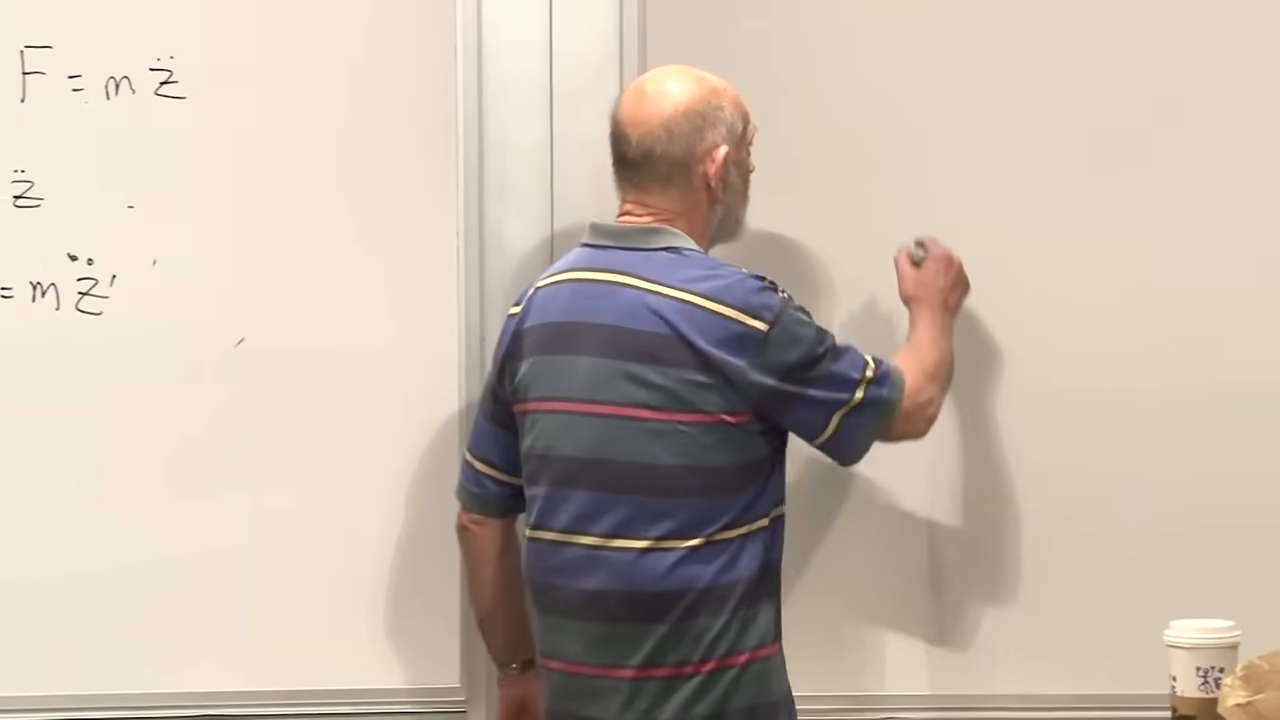
\includegraphics[width=\linewidth]{lecture_01_figure_02.png}
\caption{Équation de Newton dans deux référentiels de coordonnées en mouvement uniforme l’un par rapport à l’autre.}
\par\smallskip
\textit{Cadre du cours : 00:11:50.}
\end{figure}

Accélérons maintenant l’ascenseur vers le haut à accélération constante \(g\) :
\begin{equation}
 L(t)=\frac12gt^2,\qquad
 \dot L=gt,\qquad
 \ddot L=g.
\end{equation}
La transformation de coordonnées devient
\begin{equation}
 z'=z-\frac12gt^2,
\qquad
 \ddot z'=\ddot z-g.
\label{eq:accelerated-map}
\end{equation}
En substituant dans la loi de Newton, on obtient
\begin{equation}
 F=m(\ddot z'+g),
\qquad
 m\ddot z'=F-mg.
\label{eq:fictitious-gravity}
\end{equation}
La dérivation permet de vérifier utilement le signe en cours de route : \(+mg\) apparaît d’abord du côté de l’accélération et ne devient \(-mg\) que lorsqu’on le reporte du côté de la force. Dans le référentiel dont le plancher accélère vers le haut, le terme final est dirigé vers le bas.

\begin{figure}[H]
\centering
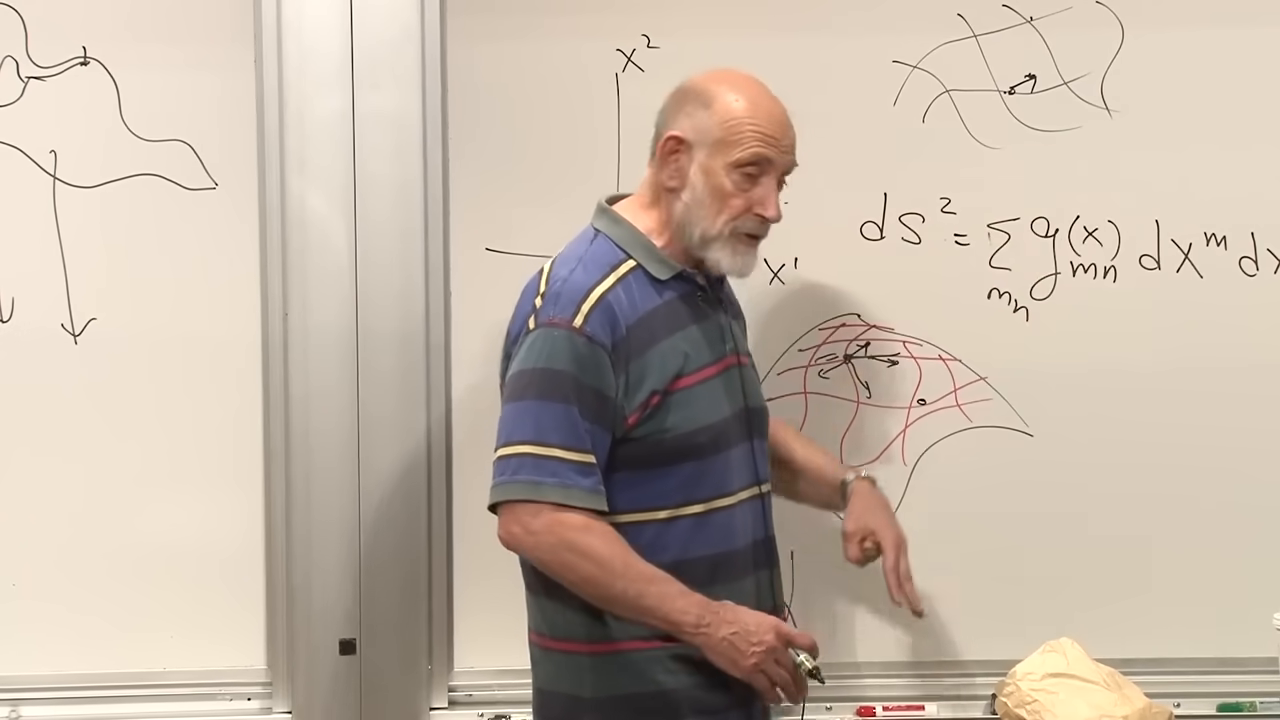
\includegraphics[width=\linewidth]{lecture_01_figure_03.png}
\caption{Transformation accélérée et force fictive qui en résulte \(-mg\).}
\par\smallskip
\textit{Cadre du cours : 00:15:35.}
\end{figure}

Le nouveau terme ressemble à la gravitation pour une raison précise : il est proportionnel à la masse. Comme la réponse inertielle est elle aussi proportionnelle à la masse, celle-ci se simplifie dans l’équation du mouvement. Un corps en chute libre suit la même trajectoire quelle que soit sa masse. L’orbite de la Terre, par exemple, est déterminée par sa position et sa vitesse dans le champ du Soleil, et non par la masse propre de la Terre dans l’approximation du corps d’épreuve.

Avant Einstein, on aurait pu écarter cette ressemblance en la considérant comme une simple curiosité. Einstein en a plutôt fait un principe : aucune expérience mécanique locale ne peut distinguer un champ gravitationnel homogène d’un référentiel accéléré de manière appropriée.

\section{Droites, coordonnées courbes et lumière}

Portons \(t\) en ordonnée et \(z\) en abscisse. Pour \(z'=z-vt\), les droites où \(z'\) est constant sont parallèles. Les lignes d’univers rectilignes restent des droites, car la transformation de coordonnées est linéaire.

\begin{figure}[H]
\centering
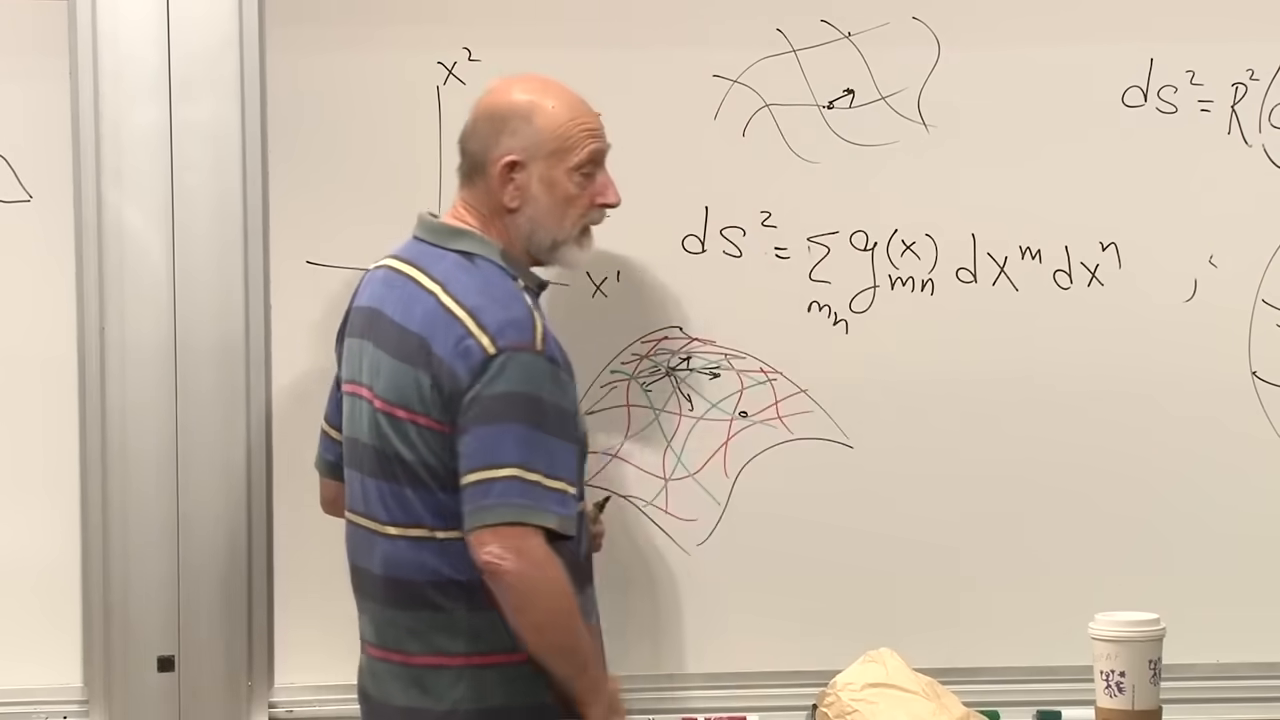
\includegraphics[width=\linewidth]{lecture_01_figure_04.png}
\caption{Réseau d’espace-temps linéaire pour des coordonnées en mouvement uniforme.}
\par\smallskip
\textit{Cadre du cours : 00:19:45.}
\end{figure}

Pour la transformation accélérée, une ligne où \(z'\) est constant vérifie
\begin{equation}
 z=z'+\frac12gt^2.
\end{equation}
C’est une parabole couchée. Si l’on prolonge le mouvement vers le passé, l’ascenseur descend en ralentissant, fait demi-tour, puis accélère vers le haut. Chaque ligne voisine où \(z'\) est constant est la même parabole, décalée horizontalement.

\begin{figure}[H]
\centering
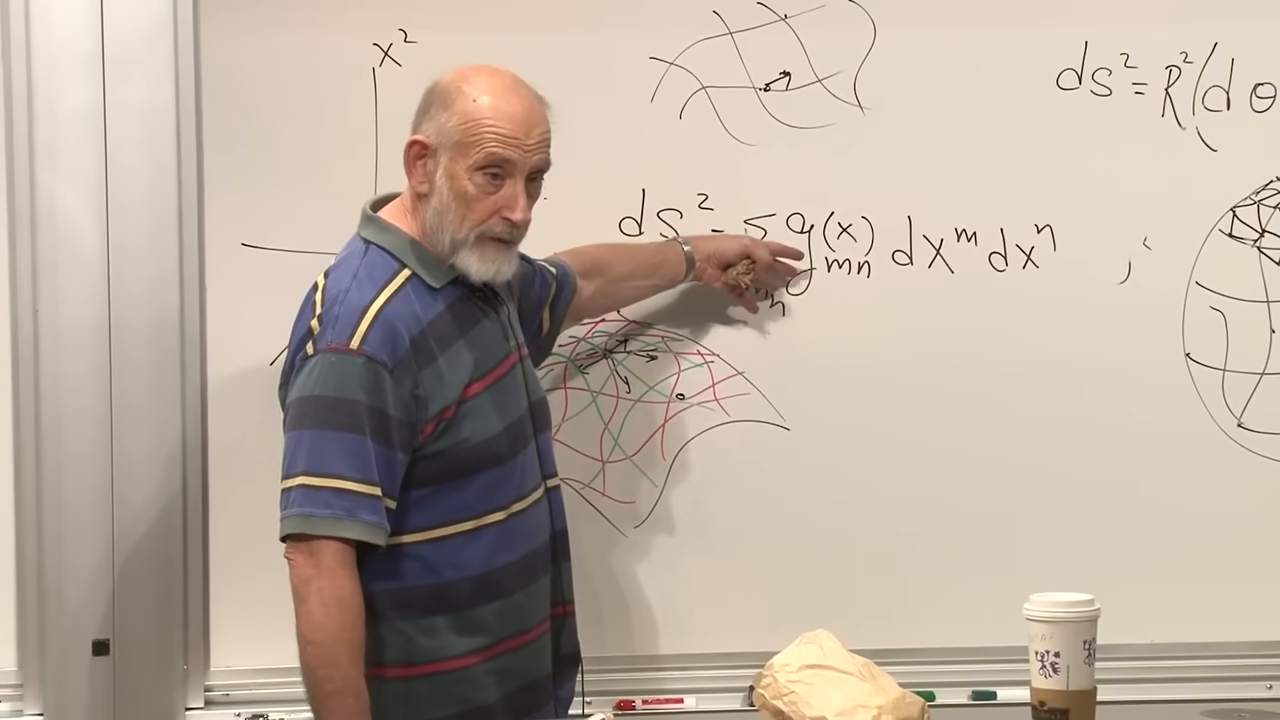
\includegraphics[width=\linewidth]{lecture_01_figure_05.png}
\caption{Courbes où \(z'\) est constant pour le système de coordonnées uniformément accéléré.}
\par\smallskip
\textit{Cadre du cours : 00:22:25.}
\end{figure}

Voici un premier indice géométrique. La relativité restreinte utilise des transformations de Lorentz linéaires, qui transforment les droites de l’espace-temps en droites de l’espace-temps. Pour représenter l’accélération et, par conséquent, imiter la gravitation, il faut des transformations curvilignes des coordonnées de l’espace-temps.

Einstein s’est servi de ce point apparemment modeste pour répondre à une question qui ne l’était pas du tout : la gravitation affecte-t-elle la lumière ? À \(t=0\), supposons que les référentiels de l’ascenseur et du sol soient momentanément au repos l’un par rapport à l’autre, puis envoyons un rayon lumineux horizontal à travers l’ascenseur. Dans le référentiel non accéléré,
\begin{equation}
 x=ct,\qquad z=0.
\end{equation}
En utilisant \(z=z'+\tfrac12gt^2\), ce même rayon, exprimé dans les coordonnées de l’ascenseur, vérifie
\begin{equation}
 z'=-\frac12gt^2
    =-\frac{g}{2c^2}x^2.
\label{eq:accelerated-light}
\end{equation}
Le rayon lumineux est rectiligne dans le référentiel inertiel et courbe dans le référentiel accéléré. Si l’accélération et la gravitation sont localement équivalentes, un champ gravitationnel doit dévier la lumière. Cet argument établit cet effet avant même qu’une équation de champ pour la gravitation ait été écrite.

\begin{figure}[H]
\centering
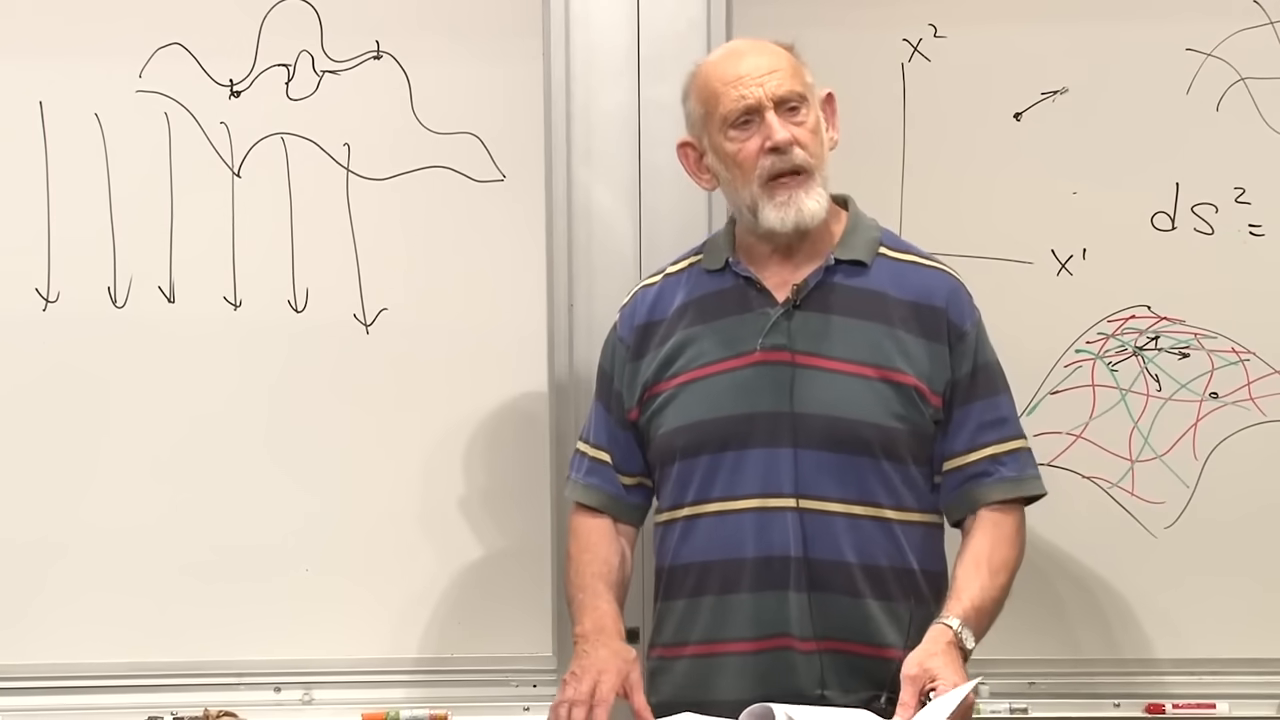
\includegraphics[width=\linewidth]{lecture_01_figure_06.png}
\caption{Rayon lumineux horizontal et trajectoire courbe dans le référentiel accéléré.}
\par\smallskip
\textit{Cadre du cours : 00:28:10.}
\end{figure}

\section{Ce qu’une transformation ne peut pas éliminer}

Un référentiel accéléré peut faire apparaître un champ gravitationnel uniforme. Cela ne signifie pas que tout champ gravitationnel soit un artefact de coordonnées. Le champ d’une étoile est dirigé radialement vers l’intérieur. Un petit laboratoire en chute libre près d’un point peut éliminer l’accélération locale, mais la même transformation ne peut éliminer le champ en tous les points autour de l’étoile.

\begin{figure}[H]
\centering
\includegraphics[width=\linewidth]{lecture_01_figure_07.png}
\caption{Champ radial et corps étendu en chute, utilisés pour mettre en évidence l’accélération de marée.}
\par\smallskip
\textit{Cadre du cours : 00:32:50.}
\end{figure}

L’obstacle est la force de marée. Imaginons une personne de deux mille miles de long qui tombe les pieds en avant. Ses pieds, plus proches de la source, accélèrent davantage que sa tête, ce qui l’étire. Tournée sur le côté, elle est comprimée, car les composantes des directions vers l’intérieur, de part et d’autre de son corps, sont orientées l’une vers l’autre. En termes newtoniens, des points voisins séparés par \(\xi^j\) acquièrent une accélération relative
\begin{equation}
 \delta a^i \simeq \partial_j g^i\,\xi^j.
\label{eq:newtonian-tide}
\end{equation}
On peut éliminer une accélération de coordonnées. En revanche, on ne peut éliminer l’accélération relative entre les points d’un corps étendu en chute libre.

\begin{classroomqa}
\audiencequestion{Des moteurs-fusées différents à la tête et aux pieds pourraient-ils simuler l’étirement et donc un champ de marée ?}
\lecturerresponse{Des moteurs appliqués peuvent certainement soumettre un corps à des contraintes, mais il s’agit alors d’une force réelle, non gravitationnelle, qui agit différemment sur ses parties. Un simple changement de coordonnées ne peut créer une accélération relative invariante entre des particules voisines en chute libre. Le diagnostic porte sur la chute libre sans force appliquée, et non sur un corps propulsé par des fusées distinctes.
\lecturetimestamp{00:36:51}}
\end{classroomqa}

Des coordonnées courbes peuvent néanmoins donner aux champs fictifs une apparence assez complexe. Un référentiel peut accélérer verticalement tout en oscillant horizontalement, ce qui produit un champ apparent dépendant du temps et comportant les deux composantes. Les coordonnées polaires ordinaires fournissent elles aussi un exemple instructif. Une particule libre qui se déplace en ligne droite dans les coordonnées cartésiennes voit d’abord \(r(t)\) diminuer, atteindre un rayon minimal, puis \(r(t)\) augmenter. Quelqu’un qui ne connaît que \(r(t)\) et \(\theta(t)\) pourrait en déduire l’existence d’une force répulsive dirigée vers l’extérieur. Dans les variantes tournantes de ces coordonnées apparaissent des termes centrifuges et de Coriolis. Ils sont proportionnels à la masse et ressemblent donc à des effets gravitationnels, mais ils ne produisent aucune déformation de marée invariante sur un corps en chute libre.

\begin{classroomqa}
\audiencequestion{Que se passe-t-il si le mouvement est décrit en coordonnées angulaires ou polaires ?}
\lecturerresponse{La description non linéaire en coordonnées donne l’impression qu’une trajectoire libre rectiligne est repoussée à partir de \(r=0\). Cette force centrifuge effective est une force de coordonnées. Le retour à un référentiel inertiel cartésien la fait disparaître et révèle qu’il n’y a aucune déformation de marée.
\lecturetimestamp{00:37:56}}
\end{classroomqa}

\begin{figure}[H]
\centering
\includegraphics[width=\linewidth]{lecture_01_figure_08.png}
\caption{Description en coordonnées polaires d’une trajectoire rectiligne, avec \(r(t)\) et \(\theta(t)\) indiqués au tableau.}
\par\smallskip
\textit{Cadre du cours : 00:40:20.}
\end{figure}

\begin{classroomqa}
\audiencequestion{Plusieurs corps gravitationnels peuvent-ils se compenser et ne laisser aucune force de marée ?}
\lecturerresponse{Les forces peuvent se compenser en un point donné, mais l’annulation de la valeur du champ n’annule généralement pas ses dérivées spatiales. Au voisinage de chaque source, les trajectoires voisines acquièrent toujours des accélérations différentes. Pour qu’il n’y ait véritablement pas de courbure, le diagnostic de marée doit être nul dans toute la région, et pas seulement la force nette en un point. \lecturetimestamp{00:42:16}}
\end{classroomqa}

\begin{classroomqa}
\audiencequestion{Comment mesure-t-on une force de marée en pratique ?}
\lecturerresponse{On laisse tomber en chute libre un objet étendu, par exemple un cristal, et l’on recherche les contraintes et déformations qui l’étirent dans une direction et le compriment dans une autre. Ces déformations sont mesurables et ne disparaissent pas quand on change les coordonnées. \lecturetimestamp{00:44:38}}
\end{classroomqa}

\begin{classroomqa}
\audiencequestion{Une personne de deux mille miles de long assise sur un manège ressentirait-elle un effet de marée radial ?}
\lecturerresponse{Une personne attachée au manège ressent des forces de soutien et peut effectivement avoir mal à la tête. Il faut plutôt que l’objet d’épreuve soit en chute libre. Sa trajectoire paraît complexe dans les coordonnées tournantes, mais reste une trajectoire rectiligne sans contrainte dans le référentiel inertiel ; la force de marée invariante est donc nulle.
\lecturetimestamp{00:45:07}}
\end{classroomqa}

\begin{classroomqa}
\audiencequestion{Peut-on incliner le corps en chute de façon que l’étirement et la compression se compensent ?}
\lecturerresponse{Aucune orientation unique ne supprime la déformation dans son ensemble. Le champ radial étire le corps selon une direction principale et le comprime selon les directions transversales. Un corps d’extension finie dans toutes les directions subit la déformation complète. \lecturetimestamp{00:47:10}}
\end{classroomqa}

\begin{figure}[H]
\centering
\includegraphics[width=\linewidth]{lecture_01_figure_09.png}
\caption{Étirement radial et compression transversale représentés ensemble pour un corps étendu en chute libre.}
\par\smallskip
\textit{Cadre du cours : 00:47:55.}
\end{figure}

\begin{classroomqa}
\audiencequestion{Les forces de marée signifient-elles que le principe d’équivalence échoue ?}
\lecturerresponse{Elles déterminent la précision avec laquelle il faut énoncer ce principe. Dans un système assez petit pour que le champ gravitationnel varie de façon négligeable à travers lui, un référentiel en chute libre permet d’éliminer la gravitation avec la précision voulue. La variation résiduelle dans un système plus étendu constitue le champ de marée. \lecturetimestamp{00:48:08}}
\end{classroomqa}

\section{De la géométrie de Minkowski à une métrique locale}

Mettons momentanément la gravitation de côté. Minkowski avait déjà montré que l’espace-temps possède une géométrie locale invariante. En une dimension spatiale, avec \(c=1\),
\begin{equation}
 d\tau^2=dt^2-dx^2.
\label{eq:minkowski-proper-time}
\end{equation}
On peut aussi définir \(ds^2=dx^2-dt^2=-d\tau^2\). La différence tient à une convention de signature, et non à une différence physique.

\begin{classroomqa}
\audiencequestion{Où intervient la vitesse de la lumière si on ne la pose pas égale à un ?}
\lecturerresponse{Si \(t\) est mesuré en unités de temps et \(x\) en unités de longueur, une forme commode est
\(d\tau^2=dt^2-dx^2/c^2\). De manière équivalente, on multiplie par \(c^2\) et l’on utilise
\(c^2d\tau^2=c^2dt^2-dx^2\). Le choix de \(ct\) ou de \(x/c\) comme coordonnée absorbe le facteur de conversion. \lecturetimestamp{00:51:02}}
\end{classroomqa}

\begin{figure}[H]
\centering
\includegraphics[width=\linewidth]{lecture_01_figure_10.png}
\caption{Intervalle de temps propre, qui établit le lien géométrique entre relativité restreinte et relativité générale.}
\par\smallskip
\textit{Cadre du cours : 00:51:10.}
\end{figure}

Einstein a reconnu que la question de savoir si un champ gravitationnel peut être éliminé ressemble à un problème étudié par Gauss pour les surfaces et par Riemann en dimensions quelconques : étant donnée une loi locale de distance, comment déterminer si la géométrie est véritablement courbe ?

En coordonnées cartésiennes euclidiennes, le théorème de Pythagore donne
\begin{equation}
 ds^2=(dx^1)^2+(dx^2)^2+\cdots
     =\delta_{mn}\,dx^m dx^n.
\label{eq:euclidean-line-element}
\end{equation}
La plage des indices correspond à la dimension de l’espace. La notation ne change pas selon qu’il y a deux, trois ou vingt-six coordonnées.

\begin{figure}[H]
\centering
\includegraphics[width=\linewidth]{lecture_01_figure_11.png}
\caption{Élément de longueur euclidien écrit comme somme de carrés des accroissements de coordonnées.}
\par\smallskip
\textit{Cadre du cours : 00:55:00.}
\end{figure}

Plaçons des coordonnées arbitraires \(x^m\) sur une surface quelconque. La distance entre deux points voisins est donnée par la forme quadratique
\begin{equation}
 ds^2=g_{mn}(x)\,dx^m dx^n.
\label{eq:general-line-element}
\end{equation}
Les fonctions \(g_{mn}(x)\) sont les composantes du tenseur métrique. La même formule s’applique aussi à une surface plane décrite en coordonnées curvilignes ; des composantes métriques non constantes ne prouvent pas, à elles seules, l’existence d’une courbure intrinsèque.

\begin{figure}[H]
\centering
\includegraphics[width=\linewidth]{lecture_01_figure_12.png}
\caption{Forme quadratique métrique générale représentée à côté d’un réseau de coordonnées courbes.}
\par\smallskip
\textit{Cadre du cours : 00:58:20.}
\end{figure}

Pour une sphère de rayon \(R\), lorsque \(\theta\) est mesuré à partir d’un pôle,
\begin{equation}
 ds^2=R^2\left(d\theta^2+\sin^2\theta\,d\phi^2\right).
\label{eq:sphere-polar}
\end{equation}
Un même accroissement de longitude couvre une grande distance près de l’équateur et une petite distance près d’un pôle ; cette dépendance à la position est précisément ce que traduit le coefficient.

\begin{classroomqa}
\audiencequestion{La latitude ordinaire étant mesurée depuis l’équateur, le coefficient ne devrait-il pas être un cosinus plutôt qu’un sinus ?}
\lecturerresponse{Oui. Si \(\lambda\) désigne la latitude mesurée depuis l’équateur, alors
\(ds^2=R^2(d\lambda^2+\cos^2\lambda\,d\phi^2)\).
L’équation \eqref{eq:sphere-polar} utilise l’angle polaire
\(\theta=\pi/2-\lambda\), mesuré depuis le pôle Nord.
\lecturetimestamp{01:01:03}}
\end{classroomqa}

\begin{figure}[H]
\centering
\includegraphics[width=\linewidth]{lecture_01_figure_13.png}
\caption{Métrique de la sphère et géométrie latitude--longitude qui déterminent son coefficient dépendant de la position.}
\par\smallskip
\textit{Cadre du cours : 01:00:30.}
\end{figure}

Des coordonnées plus générales peuvent introduire des termes croisés \(d\theta\,d\phi\), mais la distance locale reste une forme quadratique des différentielles. Les termes cubiques ou linéaires n’ont pas leur place dans un élément de longueur riemannien.

\section{Distance locale et courbure intrinsèque}

\begin{classroomqa}
\audiencequestion{La formule de la métrique donne-t-elle aussi la distance entre deux points très éloignés ?}
\lecturerresponse{Pas par simple substitution. Elle donne la distance entre des points voisins. Pour une distance macroscopique, il faut un chemin et une intégrale de \(ds\) ; si l’on entend par distance la longueur du plus court chemin, il faut également trouver ce chemin à partir de la géométrie. Plusieurs chemins localement minimaux peuvent même relier les mêmes extrémités. \lecturetimestamp{01:02:30}}
\end{classroomqa}

Sur une surface accidentée, imaginons deux piquets placés en des points éloignés et une corde tendue entre eux. La corde peut contourner une colline d’un côté ou de l’autre, et déplacer une colline change le trajet qui minimise la distance. La distance globale dépend de la géométrie entre les deux points. La distance locale est plus simple : la métrique fournit une petite règle en chaque point, et la géométrie se construit à partir de ces règles infinitésimales.

\begin{figure}[H]
\centering
\includegraphics[width=\linewidth]{lecture_01_figure_14.png}
\caption{Problème de la distance globale : un trajet tendu doit traverser la surface entre ses extrémités.}
\par\smallskip
\textit{Cadre du cours : 01:04:00.}
\end{figure}

Si l’on peut poser les éléments locaux sur un plan sans les étirer ni les déchirer, la géométrie intrinsèque est plate. Des éléments ayant les longueurs d’une sphère triangulée ne peuvent pas tous être posés à plat tout en conservant leurs arêtes. La métrique permet donc de poser un problème précis : étant donné \(g_{mn}(x)\), peut-on déterminer si ses éléments infinitésimaux s’assemblent en un espace plat ?

\begin{figure}[H]
\centering
\includegraphics[width=\linewidth]{lecture_01_figure_15.png}
\caption{La métrique et la carte locale de coordonnées, interprétées comme les éléments infinitésimaux qui composent la géométrie.}
\par\smallskip
\textit{Cadre du cours : 01:05:20.}
\end{figure}

\begin{classroomqa}
\audiencequestion{Peut-on diagnostiquer la courbure en mesurant le rapport entre la circonférence et le diamètre ?}
\lecturerresponse{Oui, c’est un test utile en deux dimensions. Sur une surface courbe, le rapport peut différer de \(\pi\). Toutefois, pour un cercle infinitésimal, l’écart n’apparaît qu’à un ordre supérieur, et cette méthode ne se généralise pas aussi simplement qu’un tenseur de courbure.
\lecturetimestamp{01:07:26}}
\end{classroomqa}

Une région est plate s’il existe un système de coordonnées dans lequel
\begin{equation}
 g_{mn}=\delta_{mn},
\qquad
 ds^2=\delta_{mn}\,dx^m dx^n
\label{eq:flat-metric}
\end{equation}
dans toute cette région. Une métrique \(g_{mn}(x)\) compliquée peut donc décrire soit un espace courbe, soit simplement des coordonnées courbes dans un espace plat. Il s’agit de savoir si une transformation de coordonnées peut éliminer toutes les complications.

\begin{figure}[H]
\centering
\includegraphics[width=\linewidth]{lecture_01_figure_16.png}
\caption{Le problème métrique posé sur une carte locale de coordonnées : peut-on transformer sa forme curviligne pour obtenir la forme plate ?}
\par\smallskip
\textit{Cadre du cours : 01:07:15.}
\end{figure}

\begin{classroomqa}
\audiencequestion{L’élément de longueur sphérique suppose-t-il que chaque petit intervalle soit plat, même si la sphère ne l’est pas ?}
\lecturerresponse{Au premier ordre, toute surface régulière est approximée en un point par son plan tangent. La courbure se manifeste dans la façon dont les approximations tangentes voisines cessent de s’ajuster les unes aux autres, ou dans les variations d’ordre supérieur à travers une carte finie. Le comportement euclidien local et la courbure globale sont donc compatibles. \lecturetimestamp{01:10:01}}
\end{classroomqa}

\begin{classroomqa}
\audiencequestion{La métrique doit-elle être continue, et que se passe-t-il au niveau d’un pli ou d’un creux ?}
\lecturerresponse{Cette discussion suppose que les cartes de coordonnées et la métrique sont suffisamment régulières pour que les dérivées requises existent. Une feuille pliée sans être étirée conserve les mêmes distances intrinsèques de part et d’autre du pli ; son apparence spectaculaire est extrinsèque. Une géométrie véritablement singulière ou non régulière demande des précautions particulières et sort du cadre régulier adopté ici. \lecturetimestamp{01:11:25}}
\end{classroomqa}

Cette distinction relève de la géométrie intrinsèque. Plier une feuille dans l’espace tridimensionnel modifie son plongement, mais pas les distances mesurées sur la feuille. Une créature confinée à la feuille, incapable de regarder l’espace dans lequel elle est plongée, peut tout de même mesurer sa géométrie intrinsèque.

\begin{figure}[H]
\centering
\includegraphics[width=\linewidth]{lecture_01_figure_17.png}
\caption{Feuille pliée permettant de distinguer la distance intrinsèque de l’apparence extrinsèque.}
\par\smallskip
\textit{Cadre du cours : 01:13:00.}
\end{figure}

\begin{classroomqa}
\audiencequestion{Pourquoi ne pas simplement diagonaliser la métrique ?}
\lecturerresponse{En un point donné, un choix approprié de coordonnées permet de diagonaliser la métrique et de la ramener à la forme locale plate. L’obstacle consiste à y parvenir dans toute une région avec un seul système de coordonnées. On ne peut pas détecter la courbure en examinant un point isolément.
\lecturetimestamp{01:13:48}}
\end{classroomqa}

\begin{figure}[H]
\centering
\includegraphics[width=\linewidth]{lecture_01_figure_18.png}
\caption{La métrique cartésienne plate \(\delta_{mn}\) écrite sous la forme quadratique locale générale.}
\par\smallskip
\textit{Cadre du cours : 01:16:00.}
\end{figure}

L’analogie avec la gravitation est maintenant exacte et non plus seulement suggestive. Une force de coordonnées peut être éliminée, tout comme on peut éliminer une description curviligne d’un espace plat. En relativité générale, l’accélération de marée se mesure par la courbure. Dans la notation qui sera introduite plus loin, des lignes d’univers voisines en chute libre vérifient l’équation de déviation géodésique
\begin{equation}
 \frac{D^2\xi^\mu}{D\tau^2}
 =-R^\mu{}_{\nu\rho\sigma}
   u^\nu\xi^\rho u^\sigma.
\label{eq:geodesic-deviation-preview}
\end{equation}
Une courbure nulle signifie qu’il n’y a pas de champ de marée invariant ; une courbure non nulle signifie qu’aucun choix de coordonnées ne peut éliminer la gravitation dans toute la région.

\section{Deux systèmes de coordonnées et un vecteur}

Pour déterminer si une métrique peut être transformée en \(\delta_{mn}\), il faut d’abord savoir comment se transforment les objets géométriques. Soient \(x^m\) et \(y^m\) deux systèmes de coordonnées réguliers définis sur la même région :
\begin{equation}
 x^m=x^m(y),\qquad y^m=y^m(x).
\label{eq:mutual-coordinate-maps}
\end{equation}
Les symboles \(x\) et \(y\) désignent des systèmes de coordonnées complets, et non deux directions spatiales particulières.

\begin{figure}[H]
\centering
\includegraphics[width=\linewidth]{lecture_01_figure_19.png}
\caption{Applications coordonnées réciproques \(x^m(y)\) et \(y^m(x)\).}
\par\smallskip
\textit{Cadre du cours : 01:20:35.}
\end{figure}

Pour des points voisins, la règle de dérivation en chaîne donne
\begin{equation}
 dy^m=\frac{\partial y^m}{\partial x^p}\,dx^p.
\label{eq:differential-transform}
\end{equation}
L’indice répété \(p\) indique une sommation. Le déplacement est un seul vecteur géométrique ; \(dx^p\) et \(dy^m\) en sont les composantes dans deux systèmes de coordonnées.

\begin{figure}[H]
\centering
\includegraphics[width=\linewidth]{lecture_01_figure_20.png}
\caption{Transformation différentielle de coordonnées obtenue par la règle de dérivation en chaîne.}
\par\smallskip
\textit{Cadre du cours : 01:22:30.}
\end{figure}

\begin{classroomqa}
\audiencequestion{Sur une grille curviligne, que représentent les lignes de coordonnées ?}
\lecturerresponse{En deux dimensions, on obtient une ligne en maintenant une coordonnée fixe tout en faisant varier l’autre. En dimensions supérieures, les ensembles où une coordonnée est constante sont des hypersurfaces. Leurs intersections locales définissent les directions de coordonnées utilisées pour décomposer les vecteurs en composantes. \lecturetimestamp{01:25:20}}
\end{classroomqa}

Un vecteur contravariant est défini par la même loi de transformation qu’un déplacement de coordonnées :
\begin{equation}
 (V')^m(y)
 =\frac{\partial y^m}{\partial x^p}\,V^p(x).
\label{eq:contravariant-vector}
\end{equation}
La vitesse le long d’une surface en est un exemple. Le vecteur ne change pas lorsque les coordonnées changent ; ses composantes, elles, changent.

\begin{figure}[H]
\centering
\includegraphics[width=\linewidth]{lecture_01_figure_21.png}
\caption{Loi de transformation d’un vecteur contravariant encadrée.}
\par\smallskip
\textit{Cadre du cours : 01:29:30.}
\end{figure}

La convention de sommation d’Einstein omet le signe de sommation lorsqu’un indice apparaît une fois en haut et une fois en bas. Cette convention facilite l’écriture des formules, mais, surtout, rend visible la structure des contractions.

\begin{classroomqa}
\audiencequestion{Fait-on des hypothèses particulières sur les systèmes de coordonnées admissibles ?}
\lecturerresponse{On suppose seulement que les deux systèmes sont liés par des fonctions et suffisamment réguliers pour que les dérivées indiquées et l’application réciproque existent dans la région considérée. On ne suppose ni linéarité ni orthogonalité. \lecturetimestamp{01:28:12}}
\end{classroomqa}

\section{Covecteurs et règle de dérivation en chaîne}

Soit \(S(x)\) un scalaire : il possède en chaque point une valeur bien définie, indépendante des étiquettes de coordonnées. La température et un champ scalaire en sont des exemples. Les composantes de son gradient sont
\begin{equation}
 W_p=\frac{\partial S}{\partial x^p}.
\label{eq:gradient-covector}
\end{equation}

\begin{figure}[H]
\centering
\includegraphics[width=\linewidth]{lecture_01_figure_22.png}
\caption{Gradient d’un scalaire présenté à côté de la loi de transformation contravariante.}
\par\smallskip
\textit{Cadre du cours : 01:31:40.}
\end{figure}

En appliquant la règle de dérivation en chaîne dans les coordonnées \(y\),
\begin{equation}
 W'_m
 =\frac{\partial S}{\partial y^m}
 =\frac{\partial x^p}{\partial y^m}
  \frac{\partial S}{\partial x^p}
 =\frac{\partial x^p}{\partial y^m}\,W_p.
\label{eq:covariant-vector}
\end{equation}
C’est la loi de transformation d’un vecteur covariant, ou covecteur. La jacobienne est l’inverse de celle de
\eqref{eq:contravariant-vector} ; les indices inférieurs et supérieurs encodent donc des comportements de transformation différents.

\begin{figure}[H]
\centering
\includegraphics[width=\linewidth]{lecture_01_figure_23.png}
\caption{Lois de transformation contravariante et covariante présentées côte à côte.}
\par\smallskip
\textit{Cadre du cours : 01:34:40.}
\end{figure}

\begin{classroomqa}
\audiencequestion{Quel est le lien entre les vecteurs covariants et contravariants ?}
\lecturerresponse{À ce stade, ils sont définis comme des objets de types différents : les déplacements et les vitesses se transforment d’une manière, les gradients de la manière inverse. La métrique fournira plus tard une application bijective qui abaisse ou relève un indice. Il ne faut pas présupposer ce lien avant d’avoir introduit la métrique. \lecturetimestamp{01:37:43}}
\end{classroomqa}

\begin{classroomqa}
\audiencequestion{La baisse d’un indice a-t-elle précédemment changé le signe de la composante temporelle ?}
\lecturerresponse{Ce signe venait de la métrique lorentzienne. Pour l’instant, la dérivation se fait d’abord en géométrie euclidienne ordinaire. La montée ou la baisse d’un indice fait toujours intervenir la métrique appropriée ; un changement de signe de la composante temporelle n’apparaît que lorsque cette métrique est de signature lorentzienne.
\lecturetimestamp{01:38:29}}
\end{classroomqa}

\begin{classroomqa}
\audiencequestion{Faut-il déjà considérer les deux lois de transformation comme deux descriptions en composantes d’un même vecteur ?}
\lecturerresponse{Pas encore. Une fois la métrique disponible, un vecteur contravariant \(V^m\) peut être converti en un covecteur \(V_m=g_{mn}V^n\). Tant que cette application n’a pas été établie, les objets à indices supérieurs et inférieurs sont logiquement distincts. \lecturetimestamp{01:39:00}}
\end{classroomqa}

Ces formules sont indépendantes de la dimension. La plage des indices change, mais pas les lois de transformation.

\section{Tenseurs à plusieurs indices}

Considérons deux vecteurs contravariants \(V^m\) et \(U^n\). Leur produit
\begin{equation}
 T^{mn}=V^mU^n
\label{eq:rank-two-product}
\end{equation}
est un tenseur contravariant de rang deux. En trois dimensions, il possède neuf composantes ; en quatre dimensions, il en possède seize. L’ordre des indices importe, sauf si une symétrie particulière est spécifiée : \(T^{mn}\) n’est pas nécessairement égal à \(T^{nm}\).

\begin{figure}[H]
\centering
\includegraphics[width=\linewidth]{lecture_01_figure_24.png}
\caption{Un tenseur de rang deux construit comme le produit de deux vecteurs contravariants.}
\par\smallskip
\textit{Image de la leçon : 01:43:40.}
\end{figure}

Chaque indice supérieur apporte un facteur de jacobienne directe :
\begin{equation}
 (T')^{mn}
 =\frac{\partial y^m}{\partial x^p}
  \frac{\partial y^n}{\partial x^q}
  T^{pq}.
\label{eq:rank-two-contravariant}
\end{equation}
La construction par produit motive cette règle, mais c’est la loi de transformation qui définit un tenseur. Un tenseur contravariant de rang trois acquiert trois facteurs de jacobienne de ce type.

\begin{figure}[H]
\centering
\includegraphics[width=\linewidth]{lecture_01_figure_25.png}
\caption{Les deux facteurs de jacobienne dans la transformation de \(T^{mn}\).}
\par\smallskip
\textit{Image de la leçon : 01:44:20.}
\end{figure}

De même, chaque indice inférieur apporte un facteur de jacobienne inverse :
\begin{equation}
 T'_{mn}
 =\frac{\partial x^p}{\partial y^m}
  \frac{\partial x^q}{\partial y^n}
  T_{pq}.
\label{eq:rank-two-covariant}
\end{equation}
Un tenseur mixte comporte un facteur de chaque type.

\begin{figure}[H]
\centering
\includegraphics[width=\linewidth]{lecture_01_figure_26.png}
\caption{La loi de transformation complète d’un tenseur à deux indices covariants.}
\par\smallskip
\textit{Image de la leçon : 01:47:30.}
\end{figure}

Le même mécanisme de transformation s’applique maintenant à la métrique. Puisque l’intervalle est un scalaire, il doit avoir la même valeur dans les deux systèmes de coordonnées :
\begin{align}
 ds^2
 &=g_{mn}(x)\,dx^m dx^n,\\
 dx^m
 &=\frac{\partial x^m}{\partial y^p}\,dy^p.
\end{align}
La substitution complète la ligne laissée inachevée au tableau :
\begin{equation}
 g'_{pq}(y)
 =\frac{\partial x^m}{\partial y^p}
  \frac{\partial x^n}{\partial y^q}
  g_{mn}(x(y)).
\label{eq:l1-metric-transformation}
\end{equation}
Ainsi, \(g_{mn}\) est un tenseur covariant de rang deux.

\begin{figure}[H]
\centering
\includegraphics[width=\linewidth]{lecture_01_figure_27.png}
\caption{La transformation de la métrique, amorcée à partir de l’invariance de l’élément de ligne à la fin de la leçon.}
\par\smallskip
\textit{Image de la leçon : 01:48:40.}
\end{figure}

La question physique posée au départ est désormais devenue une question mathématique. Étant donné \(g_{mn}(x)\), existe-t-il une transformation de coordonnées telle que \(g'_{mn}=\delta_{mn}\) dans toute la région ? Si oui, la complexité apparente n’est qu’une complexité due aux coordonnées. Sinon, l’obstacle est la courbure, et dans l’espace-temps cet obstacle constitue le contenu invariant de la gravité.
\graphicspath{{../../../generated_course_notes/core/general_relativity/2012_fall_theoretical_minimum/chapters/lecture_02/}{../../../generated_course_notes/core/general_relativity/2012_fall_theoretical_minimum/figures/}{../../../generated_course_notes/core/general_relativity/2012_fall_theoretical_minimum/assets/}}
\chapter{Géométrie intrinsèque et algèbre des tenseurs}

La notation tensorielle n’est utile que si elle nous aide à raisonner.
Une notation bien conçue fonctionne comme un jeu de pièces mécaniques : un indice supérieur s’accorde avec un indice inférieur, des objets de nature différente refusent d’être additionnés, et une contraction licite laisse un objet dont la loi de transformation se lit sur les indices restants. Ce mécanisme sert d’abord la géométrie. Nous voulons distinguer la courbure véritable de celle qui n’apparaît que parce que les coordonnées ont été déformées.

\section{Observer la courbure de l’intérieur}

Partons d’une simple feuille de papier. On peut la rouler en cylindre sans l’étirer ni la déchirer. Pour un observateur dans la pièce qui l’entoure, la feuille est manifestement courbe ; pourtant, les distances mesurées sur la feuille restent inchangées. Sa courbure extrinsèque a changé, mais pas sa géométrie intrinsèque.

Imaginons maintenant une petite créature confinée sur la feuille. Elle ne peut pas regarder la pièce environnante. Elle peut mesurer des longueurs, comparer des directions voisines, construire des triangles et transporter des règles d’un endroit à un autre. La géométrie ne devrait exiger que ces expériences internes. En gravitation, la question correspondante est de savoir si un champ représente une véritable courbure de l’espace-temps ou seulement une description curviligne d’un espace-temps plat.

Pour rendre concrète cette approche intrinsèque, remplaçons la surface par un réseau de points et de liens. Relions les points voisins, relevons la longueur de chaque lien et laissons les articulations pivoter. Un réseau triangulaire équilatéral est plat. Le pivotement des articulations ne modifie pas la géométrie codée, car on peut toujours remettre le réseau à plat sans changer aucune longueur.

Allongeons maintenant les six liens qui se rejoignent en un sommet, en gardant fixes les liens environnants. Le sommet central ne peut plus rester dans le plan sans que les longueurs prescrites soient modifiées. Il doit se soulever pour former une bosse. Il n’a pas fallu regarder la surface de l’extérieur pour diagnostiquer cette courbure : les distances incompatibles entre points voisins la contenaient déjà.

\begin{figure}[H]
\centering
\includegraphics[width=\linewidth]{lecture_02_figure_01.png}
\caption{Modèle de la géométrie intrinsèque par des liens triangulaires. Modifier les liens autour d’un sommet impose une bosse qu’on ne peut aplanir sans changer les longueurs.}
\lectureframe{00:06:40}
\end{figure}

\begin{classroomqa}
\audiencequestion{Quelle est donc la définition précise d’un espace plat ?}
\lecturerresponse{La réponse opérationnelle est que ses relations de distance intrinsèques peuvent être réalisées sans déformation dans une configuration euclidienne. Dans le langage développé ci-dessous, un espace riemannien est plat si l’on peut trouver, dans toute la région considérée, des coordonnées pour lesquelles la métrique est la delta de Kronecker constante. Cela est toujours possible localement en un point ; le faire sur toute une région est la condition non triviale. Le tenseur de courbure finira par exprimer cette condition sans faire référence à un choix particulier de coordonnées.
\lecturetimestamp{00:09:15}}
\end{classroomqa}

Cette réponse fait appel à la métrique avant que nous l’ayons établie. Nous nous tournons donc provisoirement vers l’analyse tensorielle plutôt que vers la courbure. Ce détour est indispensable : il faut reconnaître la métrique comme un tenseur avant de pouvoir distinguer sa dépendance aux coordonnées de la géométrie véritable.

\section{Champs et descriptions coordonnées}

En relativité générale, un tenseur est généralement un \emph{champ} tensoriel : en chaque point se trouve un tenseur, dont les composantes varient d’un point à l’autre. Un champ scalaire en est l’exemple le plus simple. La température sur une surface peut être représentée par un nombre \(S(P)\) en chaque point \(P\). Deux personnes peuvent attribuer au point des coordonnées différentes, mais elles doivent s’accorder sur la température en ce point.

\begin{figure}[H]
\centering
\includegraphics[width=\linewidth]{lecture_02_figure_02.png}
\caption{Un champ scalaire et deux étiquetages par coordonnées des mêmes points.}
\lectureframe{00:11:25}
\end{figure}

Soient \(x^m\) et \(y^m\) deux systèmes de coordonnées réguliers. Chacun associe aux points une liste ordonnée de nombres et, dans une carte où leurs domaines se chevauchent, les deux listes sont reliées par des fonctions réciproques l’une de l’autre,
\begin{equation}
 y^m=y^m(x^1,\ldots,x^d),
 \qquad
 x^m=x^m(y^1,\ldots,y^d).
\label{eq:coordinate-maps}
\end{equation}
La régularité permet de dériver les fonctions, et leur inversibilité garantit que le simple changement de coordonnées ne fait perdre ni ne confond aucun point.

\begin{figure}[H]
\centering
\includegraphics[width=\linewidth]{lecture_02_figure_03.png}
\caption{Deux applications de coordonnées régulières et inversibles décrivant la même région géométrique.}
\lectureframe{00:13:10}
\end{figure}

Pour un champ scalaire, la loi de transformation est simplement
\begin{equation}
 S'(y)=S(x).
\label{eq:scalar-law}
\end{equation}
Les fonctions figurant des deux côtés peuvent sembler différentes parce que leurs arguments diffèrent, mais leurs valeurs coïncident aux points correspondants. C’est le prototype d’un énoncé invariant.

\section{Coordonnées obliques et deux types de composantes}

Avant de définir les tenseurs généraux par leurs lois de transformation, il est utile de voir pourquoi les indices supérieurs et inférieurs d’un vecteur ne sont pas de simples variantes décoratives l’un de l’autre.

Traçons un quadrillage de coordonnées dont les axes ne sont ni perpendiculaires ni normalisés. En un point, faire varier \(x^m\) d’une unité de coordonnée produit un vecteur de base \(\mathbf e_m\). En langage des coordonnées,
\begin{equation}
 \mathbf e_m=\frac{\partial \mathbf r}{\partial x^m}.
\label{eq:coordinate-basis}
\end{equation}
Les vecteurs \(\mathbf e_m\) n’ont pas nécessairement une longueur unitaire ni des directions orthogonales.

\begin{figure}[H]
\centering
\includegraphics[width=\linewidth]{lecture_02_figure_04.png}
\caption{Quadrillage oblique et vecteurs de base associés aux coordonnées.}
\lectureframe{00:17:40}
\end{figure}

Tout vecteur \(\mathbf V\) peut se développer dans cette base :
\begin{equation}
 \mathbf V=V^m\mathbf e_m.
\label{eq:contravariant-expansion}
\end{equation}
Les nombres \(V^m\) sont les composantes \emph{contravariantes}. Ce sont les coefficients nécessaires pour construire le vecteur géométrique à partir des vecteurs de base.

\begin{figure}[H]
\centering
\includegraphics[width=\linewidth]{lecture_02_figure_05.png}
\caption{Développement d’un vecteur dans une base de coordonnées non orthogonale.}
\lectureframe{00:19:20}
\end{figure}

Il existe un autre ensemble naturel de nombres :
\begin{equation}
 V_m=\mathbf V\mathbin{\boldsymbol{\cdot}}\mathbf e_m.
\label{eq:covariant-projection}
\end{equation}
Ce sont les composantes \emph{covariantes}. Dans une base oblique, elles ne sont pas simplement les mêmes coefficients avec l’indice déplacé. En substituant \eqref{eq:contravariant-expansion}, on obtient
\begin{equation}
 V_m
 =V^n\bigl(\mathbf e_n\mathbin{\boldsymbol{\cdot}}\mathbf e_m\bigr).
\label{eq:covariant-from-basis}
\end{equation}

\begin{figure}[H]
\centering
\includegraphics[width=\linewidth]{lecture_02_figure_06.png}
\caption{Composantes covariantes obtenues en calculant les produits scalaires avec les vecteurs de base associés aux coordonnées.}
\lectureframe{00:21:10}
\end{figure}

Les produits scalaires des vecteurs de base forment la matrice de Gram
\begin{equation}
 g_{mn}=\mathbf e_m\mathbin{\boldsymbol{\cdot}}\mathbf e_n.
\label{eq:metric-gram}
\end{equation}
Par conséquent,
\begin{equation}
 V_m=g_{mn}V^n.
\label{eq:lower-vector}
\end{equation}
La métrique apparaît ici pour la première fois. Elle convertit les coefficients du développement en projections parce qu’elle encode les longueurs des vecteurs de base et leurs angles mutuels.

\begin{figure}[H]
\centering
\includegraphics[width=\linewidth]{lecture_02_figure_07.png}
\caption{La métrique comme matrice de Gram des vecteurs de base.}
\lectureframe{00:23:40}
\end{figure}

La même matrice permet de calculer la longueur :
\begin{align}
 \mathbf V\mathbin{\boldsymbol{\cdot}}\mathbf V
 &=(V^m\mathbf e_m)\mathbin{\boldsymbol{\cdot}}
   (V^n\mathbf e_n) \notag\\
 &=g_{mn}V^mV^n.
\label{eq:vector-length}
\end{align}

\begin{figure}[H]
\centering
\includegraphics[width=\linewidth]{lecture_02_figure_08.png}
\caption{Norme d’un vecteur exprimée à l’aide de la métrique et des composantes contravariantes.}
\lectureframe{00:25:00}
\end{figure}

\begin{classroomqa}
\audiencequestion{Pourquoi introduire cette construction géométrique avant les lois formelles de transformation ?}
\lecturerresponse{Elle donne aux indices un sens concret. Les composantes supérieures sont des coefficients de développement, les composantes inférieures sont des mesures linéaires du vecteur, et la métrique relie les deux. La définition formelle nous dira ensuite que ces rôles sont préservés par tout changement régulier de coordonnées. \lecturetimestamp{00:26:07}}
\end{classroomqa}

\begin{classroomqa}
\audiencequestion{Dans quels cas les composantes covariantes et contravariantes ont-elles les mêmes valeurs numériques ?}
\lecturerresponse{Dans une base euclidienne orthonormée,
\(g_{mn}=\delta_{mn}\), donc \(V_m=V^m\) composante par composante. La seule orthogonalité ne suffit pas : si les vecteurs de base ne sont pas de longueur unitaire, la métrique diagonale introduit encore des facteurs d’échelle.
\lecturetimestamp{00:26:19}}
\end{classroomqa}

Les coordonnées polaires illustrent clairement cette mise en garde. Les lignes de coordonnées radiales et angulaires se coupent à angle droit, mais une variation donnée \(d\theta\) correspond à une distance physique \(r\,d\theta\). Dans le plan,
\begin{equation}
 ds^2=dr^2+r^2d\theta^2,
\label{eq:polar-metric}
\end{equation}
la base est donc orthogonale, mais pas cartésienne.

\begin{figure}[H]
\centering
\includegraphics[width=\linewidth]{lecture_02_figure_09.png}
\caption{Coordonnées polaires : directions de coordonnées orthogonales et facteur d’échelle angulaire croissant avec le rayon.}
\lectureframe{00:28:10}
\end{figure}

\begin{classroomqa}
\audiencequestion{Les vecteurs covariants sont-ils réellement des vecteurs différents, ou s’agit-il seulement d’une seconde façon de décrire le même vecteur ?}
\lecturerresponse{Avant l’introduction d’une métrique, un vecteur et un covecteur sont deux types d’objets linéaires différents. Un vecteur appartient à l’espace tangent ; un covecteur est une forme linéaire sur cet espace. Une métrique non dégénérée établit entre eux une correspondance bijective, représentée par \(V_m=g_{mn}V^n\), mais il ne faut pas confondre cette correspondance avec une identité. \lecturetimestamp{00:29:10}}
\end{classroomqa}

\section{Les lois de transformation définissent le tenseur}

La définition formelle la plus sûre est opérationnelle : un tableau est un tenseur si ses composantes se transforment avec les facteurs jacobiens appropriés.
En dérivant \eqref{eq:coordinate-maps}, on obtient
\begin{equation}
 dy^m=\frac{\partial y^m}{\partial x^n}\,dx^n.
\label{eq:differential-law}
\end{equation}
Tout vecteur contravariant obéit à la même règle,
\begin{equation}
 V'^m(y)
 =\frac{\partial y^m}{\partial x^n}V^n(x).
\label{eq:contravariant-law}
\end{equation}

\begin{figure}[H]
\centering
\includegraphics[width=\linewidth]{lecture_02_figure_10.png}
\caption{Loi de transformation contravariante, calquée sur la transformation des différentielles de coordonnées.}
\lectureframe{00:32:50}
\end{figure}

Un covecteur se transforme avec le jacobien inverse :
\begin{equation}
 W'_m(y)
 =\frac{\partial x^n}{\partial y^m}W_n(x).
\label{eq:covariant-law}
\end{equation}
Le gradient d’un scalaire en est l’exemple standard. En appliquant la règle de dérivation en chaîne à \eqref{eq:scalar-law},
\begin{equation}
 \frac{\partial S}{\partial y^m}
 =\frac{\partial x^n}{\partial y^m}
  \frac{\partial S}{\partial x^n}.
\label{eq:gradient-law}
\end{equation}

\begin{figure}[H]
\centering
\includegraphics[width=\linewidth]{lecture_02_figure_11.png}
\caption{Transformation du gradient d’un scalaire comme covecteur, par la règle de dérivation en chaîne.}
\lectureframe{00:34:20}
\end{figure}

\begin{classroomqa}
\audiencequestion{Les composantes supérieures et inférieures ont-elles nécessairement les mêmes unités physiques ?}
\lecturerresponse{Non. Les composantes coordonnées héritent des unités et des conventions d’échelle des coordonnées et de leurs vecteurs de base. Si une coordonnée est une longueur et une autre un angle, leurs composantes peuvent même avoir des dimensions différentes. C’est la contraction complète qui est l’objet dont les dimensions physiques sont indépendantes des coordonnées.
\lecturetimestamp{00:35:41}}
\end{classroomqa}

\begin{classroomqa}
\audiencequestion{Pourquoi s’agit-il de dérivées partielles et non de dérivées ordinaires ?}
\lecturerresponse{Un champ dépend de plusieurs coordonnées. Le jacobien indique comment une fonction coordonnée varie lorsque l’un de ses arguments varie, les autres étant maintenus fixes ; ses éléments sont donc des dérivées partielles.
\lecturetimestamp{00:36:45}}
\end{classroomqa}

Le schéma s’étend maintenant mécaniquement. Chaque indice primé supérieur apporte un facteur \(\partial y/\partial x\) ; chaque indice primé inférieur apporte un facteur \(\partial x/\partial y\). Un tenseur mixte se transforme selon
\begin{equation}
 T'^m{}_n
 =
 \frac{\partial y^m}{\partial x^p}
 \frac{\partial x^q}{\partial y^n}
 T^p{}_q,
\label{eq:mixed-law}
\end{equation}
et un tenseur covariant de rang deux selon
\begin{equation}
 W'_{mn}
 =
 \frac{\partial x^p}{\partial y^m}
 \frac{\partial x^q}{\partial y^n}
 W_{pq}.
\label{eq:rank-two-covariant-law}
\end{equation}

\begin{figure}[H]
\centering
\includegraphics[width=\linewidth]{lecture_02_figure_12.png}
\caption{Loi de transformation d’un tenseur ayant un indice supérieur et un indice inférieur.}
\lectureframe{00:40:45}
\end{figure}

\begin{figure}[H]
\centering
\includegraphics[width=\linewidth]{lecture_02_figure_13.png}
\caption{Loi de transformation d’un tenseur covariant de rang deux, avec un jacobien inverse pour chaque indice inférieur.}
\lectureframe{00:42:15}
\end{figure}

Les indices répétés sont sommés, sauf indication contraire. Cette convention supprime les signes de sommation tout en conservant toute l’information nécessaire pour les reconstituer. Dans un terme, un indice muet répété doit apparaître exactement deux fois, une fois en position supérieure et une fois en position inférieure ; un indice libre apparaît une fois dans chaque terme d’une équation.

\begin{classroomqa}
\audiencequestion{Qui a introduit cette notation de sommation ?}
\lecturerresponse{On l’attribue traditionnellement à Einstein, d’où son nom de convention de sommation d’Einstein. Son intérêt ne tient pas à une anecdote historique : la disposition des indices rend immédiatement visibles les opérations tensorielles licites. \lecturetimestamp{00:43:21}}
\end{classroomqa}

\section{Équations tensorielles et vérité indépendante des coordonnées}

Les composantes varient avec les coordonnées, mais une équation tensorielle reste vraie dans tout système de coordonnées. Si deux tenseurs de même type vérifient \(W=T\), leur différence est le tenseur nul :
\begin{equation}
 W^{m\cdots}{}_{\cdots n}
 -T^{m\cdots}{}_{\cdots n}=0.
\label{eq:tensor-equality}
\end{equation}
La loi de transformation est linéaire ; des composantes nulles dans un système le restent donc dans tous les systèmes. La correspondance des indices libres des deux côtés est indispensable. Une équation entre des objets de types tensoriels différents n’a aucun sens indépendant des coordonnées.

\begin{figure}[H]
\centering
\includegraphics[width=\linewidth]{lecture_02_figure_14.png}
\caption{La correspondance des structures d’indices transforme l’égalité des composantes en une équation tensorielle valable dans tout système de coordonnées.}
\lectureframe{00:46:35}
\end{figure}

\begin{classroomqa}
\audiencequestion{Qu’est-ce qui est exactement invariant si les composantes du vecteur changent ?}
\lecturerresponse{Le tenseur géométrique et la vérité d’une équation tensorielle sont invariants ; la liste des composantes coordonnées ne l’est pas. Un scalaire est le cas particulier sans indice : sa valeur numérique en un point est donc la même dans tous les systèmes de coordonnées. \lecturetimestamp{00:47:19}}
\end{classroomqa}

\begin{classroomqa}
\audiencequestion{La norme du vecteur est-elle l’analogue invariant, et une norme nulle signifie-t-elle que le vecteur est nul ?}
\lecturerresponse{Une fois la métrique donnée, la contraction \(g_{mn}V^mV^n\) est un scalaire et donc une norme au carré invariante. En géométrie définie positive, elle ne s’annule que pour le vecteur nul. Dans un espace-temps lorentzien, un vecteur nul non nul peut avoir une norme nulle ; il faut donc distinguer ces deux affirmations. \lecturetimestamp{00:48:04}}
\end{classroomqa}

\section{Algèbre tensorielle : opérations autorisées}

Le tableau rassemble les principales opérations dont nous aurons besoin : multiplier par un scalaire, additionner ou soustraire des tenseurs de même type, former des produits tensoriels, contracter un indice supérieur avec un indice inférieur et, plus tard, dériver de façon covariante.

\begin{figure}[H]
\centering
\includegraphics[width=\linewidth]{lecture_02_figure_15.png}
\caption{Inventaire des opérations tensorielles : addition, multiplication, contraction et dérivation.}
\lectureframe{00:50:40}
\end{figure}

\begin{classroomqa}
\audiencequestion{Par rapport à quoi dériver ?}
\lecturerresponse{Par rapport à la position, donc aux coordonnées. Les dérivées ordinaires des composantes ne se transforment généralement pas comme des tenseurs, car les jacobiens varient eux-mêmes. La dérivation covariante remédie à cela, mais sa construction attendra que les préliminaires géométriques soient établis. \lecturetimestamp{00:51:49}}
\end{classroomqa}

La multiplication par un scalaire est immédiate. L’addition et la soustraction exigent des tenseurs de même type :
\begin{equation}
 C^m{}_n=A^m{}_n+B^m{}_n,
\qquad
 D^m{}_n=A^m{}_n-B^m{}_n.
\label{eq:tensor-addition}
\end{equation}
On ne peut pas additionner un vecteur à un covecteur, ni un tenseur de rang deux à un scalaire, pas plus qu’on ne peut additionner une vitesse à une aire.

\begin{figure}[H]
\centering
\includegraphics[width=\linewidth]{lecture_02_figure_16.png}
\caption{L’addition, définie composante par composante, n’est possible que pour des tenseurs ayant la même structure d’indices libres.}
\lectureframe{00:53:00}
\end{figure}

Le produit tensoriel combine tous les indices de ses facteurs. Par exemple,
\begin{equation}
 T^{mn}=V^mW^n,
\qquad
 S^m{}_n=V^mU_n.
\label{eq:tensor-products}
\end{equation}
En quatre dimensions, \(T^{mn}\) possède seize composantes. Aucun indice n’a été sommé : il s’agit donc d’un produit extérieur, et non d’un produit scalaire.

\begin{figure}[H]
\centering
\includegraphics[width=\linewidth]{lecture_02_figure_17.png}
\caption{Produit tensoriel conservant un indice libre de chacun des facteurs vectoriels.}
\lectureframe{00:55:15}
\end{figure}

\begin{classroomqa}
\audiencequestion{Le produit de deux vecteurs désigne-t-il ici le produit scalaire ?}
\lecturerresponse{Non. Un produit scalaire contracte un indice et donne un scalaire. Le produit tensoriel laisse les deux indices libres et donne donc un tenseur de rang deux. En quatre dimensions, celui-ci a seize composantes, et non une seule. \lecturetimestamp{00:56:36}}
\end{classroomqa}

\begin{classroomqa}
\audiencequestion{Puisque les valeurs des composantes commutent, permuter les deux facteurs vectoriels ne change-t-il rien ?}
\lecturerresponse{Pour des composantes scalaires ordinaires,
\(V^mW^n=W^nV^m\). Mais les places des indices dans le tenseur sont ordonnées. Si l’on permute les facteurs puis nomme \(m\) la première place et \(n\) la seconde, on obtient le tableau transposé ; \(T^{mn}\) n’est pas nécessairement égal à \(T^{nm}\).
\lecturetimestamp{00:58:52}}
\end{classroomqa}

\section{Contraction et lemme du jacobien inverse}

La règle de dérivation en chaîne est la clé de la contraction. Puisque les applications de coordonnées sont inverses l’une de l’autre,
\begin{equation}
 \frac{\partial x^b}{\partial y^m}
 \frac{\partial y^m}{\partial x^a}
 =
 \frac{\partial x^b}{\partial x^a}
 =\delta^b{}_a.
\label{eq:inverse-jacobian}
\end{equation}
Les deux matrices jacobiennes sont inverses l’une de l’autre, et leur produit est le delta de Kronecker.

\begin{figure}[H]
\centering
\includegraphics[width=\linewidth]{lecture_02_figure_18.png}
\caption{Identité du jacobien inverse, préparée comme lemme fondant la contraction tensorielle.}
\lectureframe{01:02:15}
\end{figure}

\begin{classroomqa}
\audiencequestion{De quel type d’objet s’agit-il, le jacobien inverse ?}
\lecturerresponse{C’est la matrice dérivée de l’application de coordonnées inverse. Ses éléments sont \(\partial x^b/\partial y^m\), et sa multiplication matricielle par \(\partial y^m/\partial x^a\) donne l’identité grâce à la règle de dérivation en chaîne à plusieurs variables. \lecturetimestamp{01:02:37}}
\end{classroomqa}

Une démonstration rapide rend la notation transparente. Pour toute fonction scalaire \(f\),
\begin{equation}
 \frac{\partial f}{\partial y^m}
 \frac{\partial y^m}{\partial x^a}
 =\frac{\partial f}{\partial x^a}.
\end{equation}
En choisissant \(f=x^b\), on obtient
\begin{equation}
 \frac{\partial x^b}{\partial y^m}
 \frac{\partial y^m}{\partial x^a}
 =\frac{\partial x^b}{\partial x^a}
 =\delta^b{}_a.
\end{equation}

\begin{figure}[H]
\centering
\includegraphics[width=\linewidth]{lecture_02_figure_19.png}
\caption{La règle de dérivation en chaîne réduit les jacobiens inverses au delta de Kronecker.}
\lectureframe{01:04:55}
\end{figure}

\begin{classroomqa}
\audiencequestion{\(\delta^b{}_a\) est-il l’identité uniquement dans les coordonnées cartésiennes ?}
\lecturerresponse{Non. Le tenseur mixte \(\delta^b{}_a\) représente l’application identité dans tout système de coordonnées. Une métrique euclidienne écrite sous la forme \(\delta_{ab}\) est particulière aux coordonnées cartésiennes orthonormées, mais il ne faut pas confondre cette métrique avec l’identité à indices mixtes.
\lecturetimestamp{01:04:58}}
\end{classroomqa}

Considérons maintenant un tenseur mixte \(T^m{}_n\). Sa trace transformée est
\begin{align}
 T'^m{}_m
 &=
 \frac{\partial y^m}{\partial x^a}
 \frac{\partial x^b}{\partial y^m}
 T^a{}_b \notag\\
 &=\delta^b{}_aT^a{}_b
 =T^a{}_a.
\label{eq:trace-invariant}
\end{align}
La quantité contractée n’a aucun indice libre : c’est donc un scalaire.

\begin{figure}[H]
\centering
\includegraphics[width=\linewidth]{lecture_02_figure_20.png}
\caption{Transformation d’un tenseur mixte avant la contraction des indices supérieur et inférieur.}
\lectureframe{01:07:45}
\end{figure}

\begin{figure}[H]
\centering
\includegraphics[width=\linewidth]{lecture_02_figure_21.png}
\caption{La contraction annule les jacobiens et laisse la même trace scalaire dans les deux systèmes de coordonnées.}
\lectureframe{01:10:30}
\end{figure}

\begin{classroomqa}
\audiencequestion{Après une contraction, le résultat porte-t-il encore des indices ?}
\lecturerresponse{Seule la paire contractée disparaît. Contracter les seuls indices supérieur et inférieur de \(T^m{}_n\) donne un scalaire. Dans un tenseur de rang supérieur, tous les indices non contractés restent libres.
\lecturetimestamp{01:09:00}}
\end{classroomqa}

Par exemple,
\begin{equation}
 A^{mn}{}_{pq}
 \longmapsto
 A^{mn}{}_{pn}
 =B^m{}_p
\label{eq:higher-rank-contraction}
\end{equation}
contracte \(n\) et abaisse le rang de deux unités. Les lettres précises sont des indices muets ; la règle de structure consiste à sommer sur une place supérieure et une place inférieure.

\begin{figure}[H]
\centering
\includegraphics[width=\linewidth]{lecture_02_figure_22.png}
\caption{Une contraction de rang supérieur supprime un indice supérieur et un indice inférieur tout en préservant les indices libres restants.}
\lectureframe{01:12:35}
\end{figure}

\begin{classroomqa}
\audiencequestion{Pourquoi ne pas contracter de la même façon deux indices supérieurs ou deux indices inférieurs ?}
\lecturerresponse{Deux indices supérieurs fournissent deux jacobiens de même orientation,
\(\partial y^m/\partial x^a\) et \(\partial y^m/\partial x^b\). Leur produit ne donne pas l’identité ; la somme proposée ne suit donc pas une loi de transformation tensorielle. Une métrique peut d’abord abaisser l’un des indices ; on peut alors effectuer une contraction entre un indice supérieur--et un indice inférieur. Sans ce tenseur supplémentaire, l’opération n’est pas invariante par changement de coordonnées. \lecturetimestamp{01:13:03}}
\end{classroomqa}

\begin{figure}[H]
\centering
\includegraphics[width=\linewidth]{lecture_02_figure_23.png}
\caption{La tentative de contraction entre indices de même variance laisse deux jacobiens de même orientation et ne se réduit donc pas à l’identité.}
\lectureframe{01:14:30}
\end{figure}

\begin{classroomqa}
\audiencequestion{La contraction est-elle l’équivalent tensoriel d’un produit intérieur ?}
\lecturerresponse{Une contraction associe une place vectorielle à une place covectorielle et constitue l’appariement invariant fondamental. Avec une métrique, on peut transformer deux vecteurs en une telle paire ; le produit intérieur usuel est donc l’application d’une métrique suivie d’une contraction. \lecturetimestamp{01:14:43}}
\end{classroomqa}

\begin{classroomqa}
\audiencequestion{Les deux indices contractés doivent-ils parcourir le même ensemble de valeurs ?}
\lecturerresponse{Oui. Ils se rapportent à des bases duales du même espace tangent et du même espace cotangent, de dimension \(d\). Sinon, la sommation et l’identité du jacobien inverse ne seraient pas définies.
\lecturetimestamp{01:15:13}}
\end{classroomqa}

\begin{classroomqa}
\audiencequestion{Pourquoi un tenseur nul dans un repère est-il nul dans tous les repères ?}
\lecturerresponse{Chaque composante transformée est une combinaison linéaire des composantes initiales. Toutes ces combinaisons s’annulent si toutes les composantes d’entrée sont nulles. Cette simple linéarité rend les équations tensorielles indépendantes des coordonnées. \lecturetimestamp{01:15:31}}
\end{classroomqa}

\section{La métrique à partir de la distance au carré}

Revenons maintenant à la géométrie. Pour un déplacement infinitésimal de composantes \(dx^m\), définissons le carré de sa longueur par
\begin{equation}
 ds^2=g_{mn}(x)\,dx^m dx^n.
\label{eq:line-element}
\end{equation}
Il s’agit du théorème de Pythagore généralisé. La métrique peut varier d’un point à l’autre, et les termes hors diagonale traduisent la non-orthogonalité des directions de coordonnées.

\begin{figure}[H]
\centering
\includegraphics[width=\linewidth]{lecture_02_figure_24.png}
\caption{La liste des opérations tensorielles cède la place à la définition quadratique de l’élément de ligne infinitésimal.}
\lectureframe{01:18:45}
\end{figure}

Seule la partie symétrique contribue, puisque
\(dx^m dx^n=dx^n dx^m\). Nous pouvons donc poser
\begin{equation}
 g_{mn}=g_{nm}.
\label{eq:metric-symmetry}
\end{equation}
En dimension \(d\), une métrique symétrique possède
\begin{equation}
 \frac{d(d+1)}{2}
\label{eq:metric-component-count}
\end{equation}
composantes indépendantes : dix en quatre dimensions, six en trois et trois en deux.

\begin{figure}[H]
\centering
\includegraphics[width=\linewidth]{lecture_02_figure_25.png}
\caption{Élément de ligne et tableau symétrique des composantes, utilisés pour compter les composantes indépendantes de la métrique.}
\lectureframe{01:21:35}
\end{figure}

\begin{classroomqa}
\audiencequestion{Pourquoi y a-t-il dix composantes indépendantes de la métrique en quatre dimensions, et non seize ?}
\lecturerresponse{Il y a quatre termes diagonaux et six paires hors diagonale non ordonnées. De façon équivalente,
\(4(4+1)/2=10\). La partie antisymétrique, multipliée par le produit symétrique \(dx^m dx^n\), s’annulerait. \lecturetimestamp{01:19:50}}
\end{classroomqa}

\begin{classroomqa}
\audiencequestion{Combien y a-t-il de composantes indépendantes en trois dimensions ?}
\lecturerresponse{Six : trois termes diagonaux et trois paires hors diagonale, soit \(3(3+1)/2\). \lecturetimestamp{01:20:47}}
\end{classroomqa}

\begin{classroomqa}
\audiencequestion{Et en deux dimensions ?}
\lecturerresponse{Trois : \(g_{11}\), \(g_{22}\) et l’unique paire symétrique \(g_{12}=g_{21}\). \lecturetimestamp{01:22:28}}
\end{classroomqa}

\subsection{Pourquoi la métrique est un tenseur}

La distance au carré est un scalaire. Écrire le même déplacement dans deux systèmes de coordonnées donne donc
\begin{equation}
 g_{mn}(x)\,dx^m dx^n
 =
 g'_{pq}(y)\,dy^pdy^q.
\label{eq:length-invariance}
\end{equation}
Utilisons deux fois
\begin{equation}
 dx^m=\frac{\partial x^m}{\partial y^p}\,dy^p
\end{equation}
On obtient alors
\begin{align}
 ds^2
 &=
 g_{mn}(x)
 \frac{\partial x^m}{\partial y^p}
 \frac{\partial x^n}{\partial y^q}
 dy^pdy^q.
\label{eq:metric-transform-derivation}
\end{align}
La comparaison avec l’expression primée identifie
\begin{equation}
 g'_{pq}(y)
 =
 \frac{\partial x^m}{\partial y^p}
 \frac{\partial x^n}{\partial y^q}
 g_{mn}(x).
\label{eq:metric-transformation}
\end{equation}
C’est exactement la loi de transformation d’un tenseur covariant de rang deux.

\begin{figure}[H]
\centering
\includegraphics[width=\linewidth]{lecture_02_figure_26.png}
\caption{Dérivation de la loi de transformation de la métrique à partir de l’invariance de l’élément de ligne scalaire.}
\lectureframe{01:26:25}
\end{figure}

Cette conclusion explique aussi la présence de deux indices inférieurs. Chaque indice inférieur de la métrique s’apparie avec un indice supérieur d’une composante du déplacement. Lors d’un changement de coordonnées, les deux jacobiens inverses dans \eqref{eq:metric-transformation} annulent les deux jacobiens directs des différentielles, laissant \(ds^2\) inchangé.

\section{La matrice métrique et son inverse}

En un point, \(g_{mn}\) est une matrice symétrique :
\begin{equation}
 [g_{mn}]
 =
 \begin{pmatrix}
 g_{11} & g_{12} & \cdots \\
 g_{12} & g_{22} & \cdots \\
 \vdots & \vdots & \ddots
 \end{pmatrix}.
\label{eq:metric-matrix}
\end{equation}

\begin{figure}[H]
\centering
\includegraphics[width=\linewidth]{lecture_02_figure_27.png}
\caption{La métrique représentée par une matrice symétrique, une fois établie sa loi de transformation tensorielle.}
\lectureframe{01:28:50}
\end{figure}

La métrique doit être non dégénérée : elle n’a aucune valeur propre nulle et possède donc un inverse. Notons cet inverse \(g^{mn}\).
En notation indicielle,
\begin{equation}
 g_{mn}g^{np}=\delta_m{}^p.
\label{eq:inverse-metric}
\end{equation}
L’indice répété \(n\) est sommé, tandis que \(m\) et \(p\) désignent la ligne et la colonne du produit.

\begin{figure}[H]
\centering
\includegraphics[width=\linewidth]{lecture_02_figure_28.png}
\caption{La métrique inverse introduite par la relation
\(g_{mn}g^{np}=\delta_m{}^p\).}
\lectureframe{01:31:40}
\end{figure}

\begin{classroomqa}
\audiencequestion{Où se trouvent concrètement les vecteurs et les tenseurs en un point ?}
\lecturerresponse{Les vecteurs en un point forment son espace tangent \(T_P M\) ; les covecteurs forment l’espace dual \(T_P^*M\). Les tenseurs d’ordre supérieur appartiennent à des produits tensoriels de ces espaces. Un champ tensoriel associe de façon régulière un tel objet à chaque point. La métrique est une forme bilinéaire sur l’espace tangent, et son inverse est la forme bilinéaire correspondante sur l’espace cotangent. \lecturetimestamp{01:34:15}}
\end{classroomqa}

\begin{figure}[H]
\centering
\includegraphics[width=\linewidth]{lecture_02_figure_29.png}
\caption{Vecteur représenté dans l’espace tangent attaché à un point d’une variété courbe.}
\lectureframe{01:35:45}
\end{figure}

\begin{classroomqa}
\audiencequestion{La relation \(g_{mn}g^{np}=\delta_m{}^p\) ne concerne-t-elle que le cas \(m=p\) ?}
\lecturerresponse{Non. C’est l’équation matricielle complète. Pour chaque paire ordonnée \((m,p)\), le produit sommé vaut un si \(m=p\) et zéro si \(m\ne p\). Toutes les équations diagonales et hors diagonale sont présentes simultanément. \lecturetimestamp{01:36:50}}
\end{classroomqa}

\begin{figure}[H]
\centering
\includegraphics[width=\linewidth]{lecture_02_figure_30.png}
\caption{La relation d’inversion interprétée comme l’identité complète à indices mixtes.}
\lectureframe{01:38:50}
\end{figure}

En deux dimensions, cela signifie
\begin{equation}
 \begin{pmatrix}
 g_{11} & g_{12}\\
 g_{12} & g_{22}
 \end{pmatrix}
 \begin{pmatrix}
 g^{11} & g^{12}\\
 g^{12} & g^{22}
 \end{pmatrix}
 =
 \begin{pmatrix}
 1&0\\
 0&1
 \end{pmatrix}.
\label{eq:two-dimensional-inverse}
\end{equation}
Par exemple,
\begin{align}
 g_{11}g^{11}+g_{12}g^{12}&=1,\\
 g_{11}g^{12}+g_{12}g^{22}&=0.
\end{align}
L’autre ligne fournit les deux équations restantes.

\begin{figure}[H]
\centering
\includegraphics[width=\linewidth]{lecture_02_figure_31.png}
\caption{Identité de la métrique inverse développée sous la forme d’un produit matriciel explicite en deux dimensions.}
\lectureframe{01:40:00}
\end{figure}

\begin{classroomqa}
\audiencequestion{La métrique doit-elle être définie positive ?}
\lecturerresponse{En géométrie riemannienne ordinaire, la définie-positivité garantit que le carré de toute longueur non nulle est positif. L’espace-temps utilise plutôt une métrique lorentzienne, dont un signe diffère des trois autres. Dans les deux cas, la condition requise ici est la non-dégénérescence, et non la positivité.
\lecturetimestamp{01:42:18}}
\end{classroomqa}

\begin{classroomqa}
\audiencequestion{Pourquoi exclure une valeur propre nulle ?}
\lecturerresponse{Une valeur propre nulle rend la matrice métrique singulière : \(g^{mn}\) n’existe donc pas, et la métrique ne peut pas établir de correspondance bijective entre les vecteurs et les covecteurs. Au sens habituel de la géométrie différentielle, une métrique doit être non dégénérée. \lecturetimestamp{01:43:56}}
\end{classroomqa}

\begin{classroomqa}
\audiencequestion{Les dix composantes indépendantes d’une métrique en quatre dimensions ont-elles un rapport avec la théorie des cordes à dix dimensions ?}
\lecturerresponse{Non. Le premier « dix » est simplement \(4(4+1)/2\), le nombre d’entrées d’une matrice symétrique de taille quatre sur quatre. L’apparition de dix dimensions d’espace-temps dans la théorie des supercordes a une autre origine. \lecturetimestamp{01:44:32}}
\end{classroomqa}

\begin{classroomqa}
\audiencequestion{Si l’espace-temps lorentzien possède des vecteurs non nuls de longueur nulle, la métrique est-elle alors non inversible ?}
\lecturerresponse{Non. Un vecteur nul vérifie \(g_{mn}V^mV^n=0\) : il s’agit d’une compensation au sein d’une forme quadratique indéfinie. Ce n’est pas un vecteur associé à une valeur propre nulle et vérifiant \(g_{mn}V^n=0\). Par exemple, la métrique de Minkowski a pour valeurs propres \(\pm1\) et est parfaitement inversible, tout en admettant des vecteurs de genre lumière. \lecturetimestamp{01:45:02}}
\end{classroomqa}

\section{Et maintenant}

Nous pouvons maintenant énoncer clairement le programme géométrique. La métrique décrit les distances infinitésimales, se transforme de manière covariante et possède une inverse. Ses composantes peuvent sembler compliquées simplement parce que les coordonnées le sont. Pour déterminer si la géométrie elle-même est courbe, nous devons comparer la métrique en des points voisins d’une manière indépendante des coordonnées.

Les dérivées ordinaires ne suffisent pas, car dériver un tenseur revient aussi à dériver les jacobiens, qui dépendent de la position, dans sa loi de transformation. L’étape suivante consiste donc à introduire la dérivation covariante. À partir des dérivées de la métrique, on construit une connexion ; à partir des dérivées et des produits de cette connexion, on construit la courbure. Ce n’est qu’alors que la question de la page courbée recevra sa réponse intrinsèque définitive.
\graphicspath{{../../../generated_course_notes/core/general_relativity/2012_fall_theoretical_minimum/chapters/lecture_03/}{../../../generated_course_notes/core/general_relativity/2012_fall_theoretical_minimum/figures/}{../../../generated_course_notes/core/general_relativity/2012_fall_theoretical_minimum/assets/}}
\chapter{Aplatissement local, dérivation covariante et courbure}

\lectureoverview{En un point donné, on peut toujours rendre une métrique euclidienne au premier ordre. La courbure apparaît là où cette liberté de coordonnées s’arrête : dans l’échec, au second ordre, de l’ajustement des repères locaux voisins. Nous allons développer cette idée en trois étapes. Nous commencerons par les coordonnées normales, puis étudierons la dérivée covariante et sa connexion, et enfin la non-commutativité de deux dérivées covariantes, qui définit le tenseur de Riemann et donne un sens invariant à la gravité de marée.}

\section{Le nécessaire fardeau des indices}

La relativité générale est difficile d’une manière bien particulière. Ses idées fondamentales ne sont pas d’une obscurité insurmontable, mais un calcul se retrouve vite encombré d’indices, de dérivées et de symboles. Il existe des langages plus compacts : les repères mobiles, les formes différentielles, les spineurs, les twistors et d’autres outils apparentés permettent de condenser de longues équations en composantes en objets compacts. Apprendre ces langages demande toutefois un travail considérable, et une notation compacte peut masquer les mécanismes qu’il importe le plus de comprendre lors d’une première approche.

Les équations de Maxwell en donnent un exemple. Écrites composante par composante, elles se ramènent à plusieurs équations distinctes. La notation vectorielle les rassemble sous forme d’équations de divergence et de rotationnel, ce qui rend leur structure plus facile à voir. La relativité générale admet des condensations analogues, mais la méthode des composantes reste la voie sûre lorsqu’il faut effectuer un calcul explicite. Nous conserverons donc les indices apparents. Une fois leur grammaire familière, le cheminement conceptuel devient beaucoup plus fluide, même si les calculs peuvent encore remplir des pages.

Des logiciels de calcul symbolique peuvent aider pour ces calculs. À partir d’une métrique \(g_{mn}(x)\), un tel logiciel peut construire les symboles de Christoffel, les tenseurs de Riemann, de Ricci et d’Einstein. Il peut ensuite substituer ces expressions dans les équations de champ. Cela ne dispense pas de comprendre la signification de ces objets ; cela sépare simplement le développement mécanique de la géométrie.

\begin{classroomqa}
\audiencequestion{Quels étaient les domaines de recherche actifs en relativité générale à l’époque de cette conférence ?}
\lecturerresponse{La conférence en distinguait plusieurs. La gravité quantique et la physique quantique des trous noirs étaient des problèmes centraux de la théorie fondamentale. L’astrophysique classique et la relativité numérique étudiaient des systèmes tels que des trous noirs en orbite ou en fusion, pour lesquels résoudre les équations d’Einstein et prédire le rayonnement gravitationnel exige bien davantage que de fournir aveuglément des équations à un ordinateur. Ces mêmes structures mathématiques trouvaient aussi des applications en physique de la matière condensée et en dynamique des fluides. L’évolution historique était tout aussi frappante : la relativité générale, qui relevait d’un domaine relativement restreint dans les 1960, était devenue l’un des langages centraux de la physique théorique, étroitement lié à la théorie quantique des champs.
\lecturetimestamp{00:05:15}}
\end{classroomqa}

C’est la dernière conférence consacrée à la géométrie riemannienne pour elle-même. À partir de la prochaine, la géométrie sera interprétée comme la gravité. Le lien apparaît déjà. Distinguer un véritable champ gravitationnel d’un champ apparent dû à des coordonnées accélérées ou curvilignes revient mathématiquement au même que distinguer une métrique courbe d’une métrique plate exprimée dans des coordonnées peu commodes.

\section{La question invariante}

Une géométrie bidimensionnelle est plate lorsque la géométrie euclidienne y vaut intrinsèquement : les droites, les parallèles, les relations entre les angles d’un triangle et les mesures de distance ont toutes leur forme euclidienne. On pourrait être tenté d’affirmer que la platitude signifie \(g_{mn}=\delta_{mn}\), mais cette affirmation dépend des coordonnées. Même dans le plan ordinaire, la métrique dépend de la position en coordonnées polaires. La formulation correcte est qu’une région plate admet des coordonnées dans lesquelles la métrique est constante et euclidienne dans toute la région.

Supposons plutôt que la métrique nous soit donnée dans des coordonnées quelconques. Une mauvaise méthode consisterait à passer en revue des systèmes de coordonnées, à transformer chaque fois la métrique et à espérer finir par trouver une forme cartésienne. Comme les possibilités sont infinies, ce n’est pas un critère pratique.

La bonne stratégie consiste à construire un diagnostic à partir de \(g_{mn}\) et de ses dérivées. Nous voulons un objet \(R\) ayant deux propriétés décisives :
\[
\begin{aligned}
R=0
&\quad\Longleftrightarrow\quad
\text{locally flat geometry},\\
R\neq 0 \text{ at } P
&\quad\Longrightarrow\quad
\text{curvature at } P.
\end{aligned}
\]
Surtout, \(R\) doit être un tenseur. Si un tenseur s’annule dans un système de coordonnées, il s’annule dans tous les systèmes ; il n’est donc pas nécessaire de chercher des coordonnées.

\begin{figure}[H]
\centering
\includegraphics[width=\linewidth]{lecture_03_figure_01.png}
\caption{Le test invariant recherché : la métrique n’a pas à être manifestement égale à \(\delta_{mn}\), tandis qu’un objet de courbure nul doit caractériser une géométrie localement plate.}
\lectureframe{00:18:20}
\end{figure}

La précision \emph{localement} est importante. Un tenseur de Riemann nul garantit une géométrie euclidienne locale ; des identifications globales peuvent néanmoins donner lieu à une topologie non triviale. Un cylindre plat ou un tore plat, par exemple, peut être euclidien localement sans être le plan à l’échelle globale.

\section{La géométrie métrique à petite échelle}

Il est utile de voir comment la situation change avec la dimension. Un espace de dimension zéro n’est qu’un point. Un espace riemannien connexe de dimension un peut être localement redressé en une droite ; globalement, il peut être un intervalle, une droite ou une boucle. Un insecte confiné à un circuit fermé unidimensionnel peut en mesurer la circonférence, mais le fait que le circuit soit incurvé dans une pièce ambiante ne modifie pas sa métrique intrinsèque.

En deux dimensions, la géométrie intrinsèque est bien plus riche : un plan, une sphère, une surface terrestre irrégulière et un tore peuvent différer même localement, et leurs topologies globales peuvent également être différentes. La métrique mesure les distances infinitésimales :
\begin{equation}
 ds^2=g_{mn}(x)\,dx^m dx^n.
\label{eq:l3-line-element}
\end{equation}
La quantité \(ds^2\) est un scalaire. Les variations de \(dx^m\) lors d’une transformation de coordonnées sont donc exactement compensées par la transformation de \(g_{mn}\).

\begin{figure}[H]
\centering
\includegraphics[width=\linewidth]{lecture_03_figure_02.png}
\caption{L’élément de longueur invariant exprimé à l’aide d’une métrique dépendant de la position.}
\lectureframe{00:19:00}
\end{figure}

La métrique est non dégénérée et possède donc un inverse :
\begin{equation}
 g^{mn}g_{nr}=\delta^m{}_r.
\label{eq:l3-inverse-metric}
\end{equation}
Le tenseur de Kronecker mixte \(\delta^m{}_r\) est l’application identité. En géométrie riemannienne ordinaire, la métrique est également définie positive,
\begin{equation}
 g_{mn}u^m u^n>0
\qquad\text{for every nonzero }u^m.
\label{eq:l3-positive}
\end{equation}
L’espace-temps lorentzien relâchera par la suite cette condition de positivité tout en conservant la non-dégénérescence.

\begin{figure}[H]
\centering
\includegraphics[width=\linewidth]{lecture_03_figure_03.png}
\caption{La métrique inverse et le tenseur identité au tableau.}
\lectureframe{00:20:40}
\end{figure}

La métrique établit une correspondance entre vecteurs et covecteurs :
\begin{equation}
 V_m=g_{mn}V^n,
 \qquad
 V^m=g^{mn}V_n.
\label{eq:l3-raise-lower}
\end{equation}
Changer un indice est donc une opération effectuée par la métrique, et non une simple modification typographique.

\begin{figure}[H]
\centering
\includegraphics[width=\linewidth]{lecture_03_figure_04.png}
\caption{Monter et abaisser un indice vectoriel à l’aide de la métrique et de son inverse.}
\lectureframe{00:24:40}
\end{figure}

Si toutes les composantes de \(g_{mn}\) sont constantes dans une région, un changement linéaire constant de coordonnées permet d’y diagonaliser et de normaliser la métrique. La géométrie est alors plate. Les informations intéressantes doivent donc être liées à la variation de la métrique avec la position.

\section{Coordonnées normales : aplatissement au premier ordre}

Choisissons un point \(P\). Le théorème des coordonnées normales affirme que l’on peut construire des coordonnées centrées en \(P\) telles que
\begin{align}
 g_{mn}(P)&=\delta_{mn}, \label{eq:l3-normal-metric}\\
 \partial_r g_{mn}(P)&=0. \label{eq:l3-normal-first}
\end{align}
La conférence les appelle coordonnées normales de Gauss. Géométriquement, on trace des axes passant par \(P\), puis on prolonge leurs lignes de coordonnées aussi droit que la géométrie le permet. La notion précise de rectitude sera celle du mouvement géodésique.

\begin{figure}[H]
\centering
\includegraphics[width=\linewidth]{lecture_03_figure_05.png}
\caption{Coordonnées normales choisies de sorte que la métrique soit euclidienne au point considéré.}
\lectureframe{00:28:50}
\end{figure}

Un tel repère n’est pas unique. Une rotation orthogonale en \(P\) conserve \(g_{mn}(P)=\delta_{mn}\). L’orientation des axes n’importe pas ; ce qui compte, c’est l’existence d’un repère dans lequel \eqref{eq:l3-normal-metric} et \eqref{eq:l3-normal-first} sont vérifiées toutes les deux.

\begin{classroomqa}
\audiencequestion{Ces conditions ne sont-elles vérifiées qu’au point choisi, ou dans tout un voisinage ?}
\lecturerresponse{Elles sont vérifiées au point choisi \(P\). On peut centrer un repère normal en n’importe quel point, mais on ne peut généralement pas utiliser un même système de coordonnées sur une région courbe en gardant la métrique euclidienne et toutes ses dérivées premières nulles partout. Prolonger les mêmes coordonnées au-delà de \(P\) fait apparaître des dérivées d’ordre supérieur de la métrique.
\lecturetimestamp{00:29:53}}
\end{classroomqa}

En \(P\), les dérivées secondes sont généralement inévitables :
\begin{equation}
 \partial_r\partial_s g_{mn}(P)\neq 0
 \qquad\text{in general}.
\label{eq:l3-normal-second}
\end{equation}
Ainsi, en un point, la métrique ne porte aucune information invariante sur la courbure à l’ordre zéro ou au premier ordre : la liberté de coordonnées permet de l’éliminer. Les premières informations invariantes possibles apparaissent au second ordre.

\begin{figure}[H]
\centering
\includegraphics[width=\linewidth]{lecture_03_figure_06.png}
\caption{Conditions des coordonnées normales : la métrique est euclidienne, ses dérivées premières s’annulent et ses dérivées secondes peuvent être non nulles.}
\lectureframe{00:30:50}
\end{figure}

\subsection{Pourquoi la liberté de coordonnées suffit}

Prenons \(P\) comme origine commune des coordonnées \(x^m\) et \(y^m\). Après avoir ajusté la métrique à l’origine au moyen d’une transformation linéaire, considérons la partie quadratique d’un changement de coordonnées supplémentaire :
\begin{equation}
 x^m
 =y^m+C^m{}_{nr}y^n y^r+O(y^3),
 \qquad C^m{}_{nr}=C^m{}_{rn}.
\label{eq:l3-quadratic-transform}
\end{equation}
En dimension quatre, la paire symétrique \(nr\) admet
\[
\frac{4(4+1)}{2}=10
\]
choix indépendants. Pour chacune des quatre valeurs de \(m\), il y a dix coefficients \(C^m{}_{nr}\), soit quarante coefficients quadratiques.

En dimension quatre, la métrique symétrique possède elle aussi dix composantes indépendantes. Chaque composante a quatre dérivées premières ; les conditions \(\partial_r g_{mn}(P)=0\) représentent donc quarante équations. Cette égalité montre que la liberté quadratique de changement de coordonnées a exactement la dimension voulue pour imposer les conditions sur les dérivées premières. Le théorème des coordonnées normales garantit l’existence ; le décompte constitue un contrôle structurel utile, mais ne démontre pas à lui seul qu’un système non linéaire arbitraire est résoluble.

\begin{figure}[H]
\centering
\includegraphics[width=\linewidth]{lecture_03_figure_07.png}
\caption{La transformation quadratique des coordonnées et les dix monômes quadratiques indépendants en dimension quatre.}
\lectureframe{00:33:50}
\end{figure}

\begin{classroomqa}
\audiencequestion{Est-ce une tentative de transformation de coordonnées :
\(x^m=y^m+C^m{}_{nr}y^n y^r+\cdots\)?}
\lecturerresponse{Oui. On choisit les coefficients \(C^m{}_{nr}\) de sorte que, dans les nouvelles coordonnées, les dérivées premières de la métrique s’annulent à l’origine commune. La partie linéaire maintient inversible le jacobien au voisinage de ce point, tandis que la partie quadratique ajuste les dérivées premières de la métrique.
\lecturetimestamp{00:35:41}}
\end{classroomqa}

\begin{classroomqa}
\audiencequestion{Est-ce cela que signifie l’expression « une géométrie lisse est localement plate » ?}
\lecturerresponse{C’est l’énoncé pertinent au premier ordre. À suffisamment petite échelle, une surface lisse est approximée par son plan tangent, et les coordonnées normales expriment ce fait par \(g_{mn}(P)=\delta_{mn}\) et \(\partial_r g_{mn}(P)=0\). La platitude exacte dans un voisinage est une condition plus forte : elle exige aussi que le tenseur de courbure s’y annule.
\lecturetimestamp{00:36:19}}
\end{classroomqa}

\begin{classroomqa}
\audiencequestion{L’égalité entre quarante coefficients et quarante équations garantit-elle vraiment que le système peut être résolu ?}
\lecturerresponse{Ce décompte repère la liberté de coordonnées nécessaire, tandis que le théorème garantit la construction locale pour une métrique lisse et non dégénérée. La conférence propose de vérifier directement le cas bidimensionnel à titre d’exercice. L’argument ne dépend pas de la dimension quatre ; en dimension \(d\), les mêmes propriétés de symétrie et la même liberté de coordonnées s’accordent.
\lecturetimestamp{00:36:45}}
\end{classroomqa}

\begin{classroomqa}
\audiencequestion{Pourquoi le développement ne comporte-t-il pas de terme constant, et quel est le terme du premier ordre ?}
\lecturerresponse{Le terme \(y^m\) est celui du premier ordre. Le terme constant a été omis parce que les deux origines des coordonnées ont été choisies délibérément pour représenter le même point ; ainsi, \(y=0\) implique \(x=0\). Ce choix ne restreint pas la généralité.
\lecturetimestamp{00:38:52}}
\end{classroomqa}

\section{Pourquoi la dérivation composante par composante échoue}

Considérons maintenant un champ de vecteurs covariants \(V_m(x)\). Dans des coordonnées cartésiennes rectilignes d’un espace plat, les composantes d’un vecteur géométriquement constant sont constantes. On pourrait donc tenter de définir sa dérivée par \(\partial_rV_m\). La difficulté apparaît dès que le réseau de coordonnées est courbe.

\begin{figure}[H]
\centering
\includegraphics[width=\linewidth]{lecture_03_figure_08.png}
\caption{Un réseau de coordonnées curvilignes superposé à un repère local rectiligne.}
\lectureframe{00:40:10}
\end{figure}

Plaçons le même vecteur géométrique en des points voisins. Dans un repère cartésien fixe, ses composantes ne changent pas. En revanche, dans une base curviligne, les vecteurs de base eux-mêmes tournent lorsqu’on se déplace ; la liste des composantes change donc, même si le vecteur, lui, ne change pas.

\begin{figure}[H]
\centering
\includegraphics[width=\linewidth]{lecture_03_figure_09.png}
\caption{Le même vecteur acquiert des composantes différentes en des points voisins parce que la base locale des coordonnées a tourné.}
\lectureframe{00:42:30}
\end{figure}

La condition naïve
\begin{equation}
 \partial_rV_m=0
\label{eq:l3-naive-derivative}
\end{equation}
peut donc être vraie dans un système de coordonnées et fausse dans un autre. Si \(\partial_rV_m\) était un tenseur de rang deux, cela serait impossible : son annulation dans un repère entraînerait son annulation dans tous les repères. Les dérivées partielles ordinaires des composantes d’un vecteur ne sont donc pas les composantes d’un tenseur.

\begin{figure}[H]
\centering
\includegraphics[width=\linewidth]{lecture_03_figure_10.png}
\caption{La condition naïve, délibérément posée, de dérivée nulle, à côté d’une base curviligne qui change.}
\lectureframe{00:44:00}
\end{figure}

Il nous faut une dérivée qui élimine la variation apparente due à la base tout en conservant la variation réelle du champ de vecteurs.

\section{Définition de la dérivée covariante}

La dérivation en \(P\) ne compare des valeurs que dans un voisinage arbitrairement petit de \(P\). Nous pouvons donc commencer en coordonnées normales centrées en ce point. Prenons un vecteur situé en un point voisin, ramenons-en l’origine en \(P\) et gardons ses composantes en coordonnées normales inchangées pendant ce déplacement. Comparer le vecteur ainsi transporté à celui qui se trouve déjà en \(P\), puis diviser par la séparation, donne la dérivée ordinaire dans ce repère local rectiligne.

\begin{figure}[H]
\centering
\includegraphics[width=\linewidth]{lecture_03_figure_11.png}
\caption{Comparaison locale : déplacer le vecteur du point voisin dans les coordonnées normales avant de calculer la différence.}
\lectureframe{00:46:50}
\end{figure}

Exprimons maintenant cette dérivée définie géométriquement dans des coordonnées quelconques. Deux contributions interviennent : les composantes \(V_m\) peuvent varier, et la base de coordonnées peut elle aussi varier. La structure des indices fixe la forme du terme correctif :
\begin{equation}
 \nabla_rV_m
 =\partial_rV_m-\Gamma^t{}_{rm}V_t.
\label{eq:l3-covector-derivative}
\end{equation}
Les quantités \(\Gamma^t{}_{rm}\) sont les coefficients de connexion, également appelés symboles de Christoffel. Le signe moins convient à un indice vectoriel inférieur. Au centre \(P\) des coordonnées normales,
\begin{equation}
 \Gamma^t{}_{rm}(P)=0,
\qquad
 \nabla_rV_m(P)=\partial_rV_m(P).
\label{eq:l3-gamma-normal-zero}
\end{equation}

\begin{figure}[H]
\centering
\includegraphics[width=\linewidth]{lecture_03_figure_12.png}
\caption{Dérivée covariante d’un covecteur : variation ordinaire des composantes moins la variation induite par le déplacement de la base.}
\lectureframe{00:49:50}
\end{figure}

\begin{classroomqa}
\audiencequestion{La relation \(\nabla_rV_m=\partial_rV_m-\Gamma^t{}_{rm}V_t\) est-elle valable dans des coordonnées quelconques, et que devient-elle en coordonnées normales ?}
\lecturerresponse{La formule complète est valable dans des coordonnées quelconques. Au point choisi, en coordonnées normales, les dérivées premières de la métrique s’annulent, tout comme les symboles de Christoffel ; il ne reste donc que \(\partial_rV_m\). En dehors de ce point, les coefficients de connexion sont généralement non nuls, même dans ce même système de coordonnées normales.
\lecturetimestamp{00:50:22}}
\end{classroomqa}

La dérivée covariante porte ce nom parce que l’objet entier \(\nabla_rV_m\) se transforme de façon covariante en tant que tenseur ; ce nom ne fait pas simplement référence à l’indice inférieur de dérivation. Le terme de Christoffel corrige précisément la loi de transformation non tensorielle de la dérivée partielle.

\begin{figure}[H]
\centering
\includegraphics[width=\linewidth]{lecture_03_figure_13.png}
\caption{La dérivée complète d’un covecteur et son terme correctif de connexion.}
\lectureframe{00:51:30}
\end{figure}

\begin{classroomqa}
\audiencequestion{Y a-t-il un lien avec la dérivée convective utilisée en mécanique des fluides ?}
\lecturerresponse{La réponse de la conférence est prudente : il existe un lien. En mécanique des fluides aussi, on distingue la variation transportée par un écoulement de celle observée en un point fixe des coordonnées, et les dérivées covariantes interviennent dans les équations des fluides sur des coordonnées ou des espaces courbes. Par définition, ces opérateurs ne sont pas identiques, mais ils corrigent tous deux une dérivée naïve pour tenir compte d’une structure qui se déplace avec la description.
\lecturetimestamp{00:52:31}}
\end{classroomqa}

Pour la connexion sans torsion utilisée ici,
\begin{equation}
 \Gamma^t{}_{rm}=\Gamma^t{}_{mr}.
\label{eq:l3-torsion-free}
\end{equation}
Des géométries plus générales peuvent comporter de la torsion et ne pas satisfaire cette symétrie. La connexion considérée ici est celle qui intervient dans la formulation métrique standard de la relativité générale.

\begin{figure}[H]
\centering
\includegraphics[width=\linewidth]{lecture_03_figure_14.png}
\caption{Les symboles de Christoffel, identifiés aux coefficients symétriques de la connexion sans torsion.}
\lectureframe{00:54:30}
\end{figure}

Une analogie physique est utile. Les coordonnées normales jouent le rôle d’un repère en chute libre en un événement : la correction de coordonnées peut y être rendue nulle. Des coordonnées curvilignes quelconques évoquent un ascenseur accéléré, où des forces apparentes apparaissent parce que le repère lui-même change. L’analogie est locale ; la courbure mesurera pourquoi un seul repère en chute libre ne peut éliminer la gravité dans toute une région étendue.

\subsection{Une correction pour chaque indice tensoriel}

Pour un tenseur covariant de rang deux \(T_{mn}\), chaque indice inférieur reçoit son propre terme correctif de connexion :
\begin{equation}
 \nabla_sT_{mn}
 =\partial_sT_{mn}
 -\Gamma^t{}_{sm}T_{tn}
 -\Gamma^t{}_{sn}T_{mt}.
\label{eq:l3-rank-two-derivative}
\end{equation}
Pour retenir la règle, gardez un indice fixe comme spectateur pendant que vous dérivez par rapport à l’autre, puis répétez l’opération pour le second indice. Les indices contravariants reçoivent des termes correspondants de signe opposé.

\begin{figure}[H]
\centering
\includegraphics[width=\linewidth]{lecture_03_figure_15.png}
\caption{Dérivée covariante d’un tenseur covariant de rang deux, avec une correction de Christoffel pour chacun des indices inférieurs.}
\lectureframe{01:01:50}
\end{figure}

\begin{classroomqa}
\audiencequestion{Le symbole \(\partial_r\) désigne-t-il uniquement les coordonnées normales, et la formule tensorielle se limite-t-elle à ce repère ?}
\lecturerresponse{Non. La notation \(\partial_r=\partial/\partial x^r\) a un sens dans n’importe quel système de coordonnées, et la formule complète de la dérivée covariante s’écrit pour des coordonnées quelconques. Les termes correctifs de Christoffel ne s’annulent qu’au point choisi d’un repère normal.
\lecturetimestamp{00:57:22}}
\end{classroomqa}

\begin{classroomqa}
\audiencequestion{Lorsque la dérivée covariante se réduit à la dérivée partielle en coordonnées normales, cette réduction ne vaut-elle qu’au point choisi ? Les symboles de Christoffel sont-ils des tenseurs ?}
\lecturerresponse{Oui, la réduction est ponctuelle. Les symboles de Christoffel ne sont pas des tenseurs : ils peuvent s’annuler en \(P\) dans des coordonnées normales et être non nuls au même point dans un autre système de coordonnées. Leur loi de transformation non tensorielle permet précisément à la combinaison dans \eqref{eq:l3-covector-derivative} de se transformer comme un tenseur.
\lecturetimestamp{00:58:13}}
\end{classroomqa}

\begin{classroomqa}
\audiencequestion{À quoi servira concrètement la dérivée covariante ?}
\lecturerresponse{Aux équations de champ. Les champs gravitationnels varient d’un point à l’autre ; leurs équations doivent donc contenir des dérivées. En même temps, ces équations doivent avoir le même contenu dans tous les systèmes de coordonnées. La dérivation covariante transforme les tenseurs en tenseurs et permet ainsi d’écrire des équations différentielles dont la validité ne dépend pas d’un repère particulier.
\lecturetimestamp{01:02:35}}
\end{classroomqa}

\begin{classroomqa}
\audiencequestion{Peut-on multiplier la dérivée covariante par un différentiel de coordonnées pour décrire la variation entre des points voisins ?}
\lecturerresponse{Oui. Le long d’un déplacement infinitésimal \(dx^s\), la variation covariante est \(dx^s\nabla_sT\). Le terme partiel mesure la variation des composantes, tandis que les termes de connexion rendent compte de la variation de la base de coordonnées. Même dans l’espace plat exprimé en coordonnées polaires, cette distinction est nécessaire.
\lecturetimestamp{01:03:22}}
\end{classroomqa}

\section{La compatibilité avec la métrique détermine la connexion}

Appliquons la règle du tenseur de rang deux à la métrique. En \(P\), dans des coordonnées normales, \(\partial_sg_{mn}=0\) et \(\Gamma^t{}_{sm}=0\), donc \(\nabla_sg_{mn}=0\). Comme la dérivée covariante est un tenseur, ce résultat ponctuel vaut dans tous les systèmes de coordonnées :
\begin{equation}
 \nabla_sg_{mn}=0.
\label{eq:l3-metric-compatibility}
\end{equation}
C’est la compatibilité avec la métrique. Elle signifie que le transport parallèle préserve la métrique, et donc les longueurs et les angles.

\begin{figure}[H]
\centering
\includegraphics[width=\linewidth]{lecture_03_figure_16.png}
\caption{L’équation de compatibilité avec la métrique ouvre la dérivation de la connexion à partir de la métrique.}
\lectureframe{01:06:20}
\end{figure}

En développant \eqref{eq:l3-metric-compatibility}, on obtient
\begin{equation}
 0
 =\partial_sg_{mn}
 -\Gamma^t{}_{sm}g_{tn}
 -\Gamma^t{}_{sn}g_{mt}.
\label{eq:l3-compat-expanded}
\end{equation}
Écrivons encore deux copies en permutant cycliquement les indices de dérivation et de la métrique :
\begin{align}
 0
 &=\partial_mg_{sn}
 -\Gamma^t{}_{ms}g_{tn}
 -\Gamma^t{}_{mn}g_{st},
\label{eq:l3-compat-m}\\
 0
 &=\partial_ng_{sm}
 -\Gamma^t{}_{ns}g_{tm}
 -\Gamma^t{}_{nm}g_{st}.
\label{eq:l3-compat-n}
\end{align}

\begin{figure}[H]
\centering
\includegraphics[width=\linewidth]{lecture_03_figure_17.png}
\caption{Trois équations de compatibilité avec la métrique, avec permutation des indices.}
\lectureframe{01:10:20}
\end{figure}

Additionnons \eqref{eq:l3-compat-m} et \eqref{eq:l3-compat-n}, puis soustrayons \eqref{eq:l3-compat-expanded}. En utilisant la symétrie sans torsion \eqref{eq:l3-torsion-free}, les termes de connexion indésirables s’annulent :
\begin{equation}
 \partial_mg_{sn}+\partial_ng_{sm}-\partial_sg_{mn}
 =2\Gamma^t{}_{mn}g_{st}.
\label{eq:l3-isolate-gamma-lowered}
\end{equation}

\begin{figure}[H]
\centering
\includegraphics[width=\linewidth]{lecture_03_figure_18.png}
\caption{L’addition de deux équations de compatibilité et la soustraction de la troisième annulent les termes de Christoffel indésirables.}
\lectureframe{01:12:10}
\end{figure}

En multipliant par \(g^{rs}\), on isole la connexion :
\begin{equation}
 \boxed{
 \Gamma^r{}_{mn}
 =\frac12 g^{rs}
 \left(
 \partial_mg_{sn}
 +\partial_ng_{sm}
 -\partial_sg_{mn}
 \right)}
\label{eq:l3-christoffel}
\end{equation}
La connexion de Levi-Civita est donc construite à partir de la métrique et de ses dérivées premières. Voilà pourquoi les symboles de Christoffel s’annulent au centre des coordonnées normales.

\begin{figure}[H]
\centering
\includegraphics[width=\linewidth]{lecture_03_figure_19.png}
\caption{La métrique inverse permet d’isoler le symbole de Christoffel dans l’équation de connexion avec indice abaissé.}
\lectureframe{01:16:10}
\end{figure}

\begin{classroomqa}
\audiencequestion{Pourquoi a-t-on posé à zéro les trois équations de compatibilité avec la métrique ?}
\lecturerresponse{Au point choisi, en coordonnées normales, les dérivées ordinaires de la métrique s’annulent, de même que les symboles de Christoffel. La dérivée covariante de la métrique y est donc nulle. Pour établir cette propriété en un autre point, centrons un repère normal en ce point et recommençons. Puisque \(\nabla_sg_{mn}\) est un tenseur, son annulation est indépendante des coordonnées.
\lecturetimestamp{01:14:27}}
\end{classroomqa}

\begin{classroomqa}
\audiencequestion{Quelles sont les dimensions de la métrique et du tableau des symboles de Christoffel, et pourquoi y a-t-il quarante composantes de Christoffel indépendantes en dimension quatre ?}
\lecturerresponse{En dimension \(d\), \(g_{mn}\) est une matrice symétrique de taille \(d\times d\). La connexion a trois indices. Pour chaque indice supérieur fixé \(r\), la paire inférieure symétrique \(mn\) offre \(d(d+1)/2\) possibilités. Une connexion sans torsion possède donc \(d^2(d+1)/2\) composantes indépendantes, soit quarante lorsque \(d=4\).
\lecturetimestamp{01:16:18}}
\end{classroomqa}

\begin{figure}[H]
\centering
\includegraphics[width=\linewidth]{lecture_03_figure_20.png}
\caption{Le tableau pendant le décompte des composantes : dix possibilités pour la paire inférieure symétrique et quatre possibilités pour l’indice supérieur.}
\lectureframe{01:16:30}
\end{figure}

\begin{classroomqa}
\audiencequestion{Quelle métrique intervient dans \eqref{eq:l3-christoffel} ? Faut-il utiliser une métrique en coordonnées normales différente en chaque point ?}
\lecturerresponse{La formule utilise les composantes de la métrique dans les coordonnées globales ou locales choisies pour le calcul. Les coordonnées normales ne sont qu’un outil local servant à dériver la règle : on passe à un repère normal en un point, on y effectue la dérivation, on transforme le résultat en retour, puis on abandonne ce repère auxiliaire. Une fois \eqref{eq:l3-christoffel} connue, on l’évalue directement dans les coordonnées quelconques qui nous intéressent.
\lecturetimestamp{01:17:21}}
\end{classroomqa}

\begin{classroomqa}
\audiencequestion{Ni \(\nabla_sg_{mn}=0\) ni la formule de Christoffel n’indiquent-ils que l’espace est plat ?}
\lecturerresponse{Non. La compatibilité avec la métrique vaut pour toute connexion de Levi-Civita, que l’espace soit courbe ou plat. Les symboles de Christoffel peuvent être non nuls même dans un plan plat exprimé en coordonnées polaires. Si tous les \(\Gamma^r{}_{mn}\) s’annulent dans toute une région pour un même système de coordonnées, ce système est cartésien dans cette région, qui est alors plate ; mais leur seule non-annulation ne révèle pas la courbure. Il faut encore un tenseur construit à partir des dérivées et des produits de \(\Gamma\).
\lecturetimestamp{01:19:27}}
\end{classroomqa}

\section{Le cône révèle ce que la connexion ne peut déterminer}

Considérons un cône arrondi. À l’écart de sa pointe, on peut l’approximer par un cône ordinaire fait de papier. Découpons un secteur dans un disque plat et collons ensemble les bords mis à nu. Le papier restant n’a subi aucun étirement ; localement, chaque point éloigné de la ligne de jonction et de la pointe demeure plat. Le secteur manquant est caractérisé par un angle de déficit \(\Delta\).

\begin{figure}[H]
\centering
\includegraphics[width=\linewidth]{lecture_03_figure_21.png}
\caption{Le cône illustre une géométrie localement plate loin de sa pointe, mais dont la courbure non triviale est concentrée en celle-ci.}
\lectureframe{01:23:00}
\end{figure}

\begin{figure}[H]
\centering
\includegraphics[width=\linewidth]{lecture_03_figure_22.png}
\caption{La découpe d’un secteur dans un disque, suivie de l’identification de ses bords, produit l’angle de déficit conique.}
\lectureframe{01:24:20}
\end{figure}

La construction en papier rend cette distinction tangible. Sur la feuille découpée, transportons un vecteur en le gardant parallèle dans le plan ordinaire. Après avoir joint les bords de la découpe, un parcours qui fait le tour de la pointe ramène le vecteur à son point de départ, mais sa direction est tournée par rapport à sa direction initiale.

\begin{figure}[H]
\centering
\includegraphics[width=0.78\linewidth]{lecture_03_figure_23.png}
\caption{Démonstration du cône en papier : une feuille plane dont on a retiré un secteur devient un cône lorsque ses bords découpés sont réunis.}
\lectureframe{01:25:10}
\end{figure}

\begin{figure}[H]
\centering
\includegraphics[width=\linewidth]{lecture_03_figure_24.png}
\caption{Vecteurs tracés sur le secteur découpé avant que ses bords soient réunis.}
\lectureframe{01:27:40}
\end{figure}

Cette rotation est l’holonomie. Elle ne résulte pas d’un mauvais choix de coordonnées le long d’un segment. Chaque petit segment peut être traité dans un repère localement plat. L’effet n’apparaît qu’après composition de ces comparaisons locales le long d’une boucle fermée. Pour le cône idéal, la rotation totale est égale à l’angle de déficit, au signe près selon l’orientation.

\begin{figure}[H]
\centering
\includegraphics[width=\linewidth]{lecture_03_figure_25.png}
\caption{Le transport parallèle autour de la pointe conique ramène un vecteur avec une direction tournée : l’holonomie enregistre la courbure enfermée.}
\lectureframe{01:29:10}
\end{figure}

\section{Deux parcours autour d’une boucle infinitésimale}

Remplaçons la boucle finie par un minuscule rectangle de coordonnées. En partant d’un sommet, effectuons d’abord le transport dans la direction \(r\), puis dans la direction \(s\). Comparons ce résultat à celui obtenu en effectuant d’abord le transport dans la direction \(s\), puis dans la direction \(r\). En coordonnées cartésiennes plates, les deux parcours donnent le même résultat. Dans une géométrie courbe, ce n’est généralement pas le cas.

\begin{figure}[H]
\centering
\includegraphics[width=\linewidth]{lecture_03_figure_26.png}
\caption{Deux ordres de transport infinitésimal autour d’un rectangle de coordonnées.}
\lectureframe{01:31:40}
\end{figure}

La mesure algébrique est le commutateur des dérivées covariantes :
\begin{equation}
 \left(\nabla_s\nabla_r-\nabla_r\nabla_s\right)V_n.
\label{eq:l3-commutator}
\end{equation}
Les dérivées partielles mixtes ordinaires commutent sur les fonctions régulières. Ici, le défaut de commutation vient de la dérivation des termes de connexion aussi bien que des composantes du vecteur.

\begin{figure}[H]
\centering
\includegraphics[width=\linewidth]{lecture_03_figure_27.png}
\caption{La boucle infinitésimale représentée par la différence entre les deux ordres de dérivation covariante.}
\lectureframe{01:33:20}
\end{figure}

Pour effectuer ce calcul, considérons d’abord
\[
 T_{rn}=\nabla_rV_n
\]
comme un tenseur covariant de rang deux. Utilisons ensuite
\eqref{eq:l3-rank-two-derivative} pour dériver \(T_{rn}\) dans la direction \(s\). Recommençons en échangeant \(r\) et \(s\), puis soustrayons les deux résultats. Le calcul est long, mais mécanique : développons, appliquons la règle du produit et simplifions les termes contenant les dérivées partielles secondes de \(V_n\).

\begin{figure}[H]
\centering
\includegraphics[width=\linewidth]{lecture_03_figure_28.png}
\caption{Début de la dérivée covariante seconde, en traitant \(\nabla_rV_n\) comme un tenseur de rang deux.}
\lectureframe{01:35:40}
\end{figure}

Avec la convention adoptée au tableau, on obtient
\begin{equation}
 \left(\nabla_s\nabla_r-\nabla_r\nabla_s\right)V_n
 =R_{srn}{}^tV_t.
\label{eq:l3-riemann-commutator}
\end{equation}

\begin{figure}[H]
\centering
\includegraphics[width=\linewidth]{lecture_03_figure_29.png}
\caption{Le commutateur des dérivées covariantes définit l’action du tenseur de courbure sur un covecteur.}
\lectureframe{01:38:30}
\end{figure}

Pour cet ordre des termes dans le commutateur,
\begin{equation}
\begin{split}
 R_{srn}{}^t
={}&
 \partial_r\Gamma^t{}_{sn}
 -\partial_s\Gamma^t{}_{rn}\\
&+\Gamma^p{}_{sn}\Gamma^t{}_{pr}
 -\Gamma^p{}_{rn}\Gamma^t{}_{ps}.
\end{split}
\label{eq:l3-riemann}
\end{equation}
D’autres textes peuvent adopter le signe opposé ou disposer les indices différemment ; la convention est fixée en écrivant à la fois \eqref{eq:l3-riemann-commutator} et \eqref{eq:l3-riemann}.

\begin{figure}[H]
\centering
\includegraphics[width=\linewidth]{lecture_03_figure_30.png}
\caption{Le tenseur de Riemann : deux dérivées de la connexion et deux termes quadratiques en la connexion.}
\lectureframe{01:39:40}
\end{figure}

L’équation \eqref{eq:l3-christoffel} montre pourquoi la courbure apparaît dès le second ordre de la métrique. Chaque \(\Gamma\) contient une dérivée première de \(g\). Les termes dérivés de \eqref{eq:l3-riemann} contiennent donc des dérivées secondes de \(g\), tandis que les termes quadratiques contiennent des produits de dérivées premières. En coordonnées normales en \(P\), la connexion elle-même s’annule, mais ses dérivées ne s’annulent généralement pas : la courbure subsiste donc :
\[
\begin{aligned}
 \Gamma^t{}_{mn}(P)&=0,\\
 R_{srn}{}^t(P)
 &=\partial_r\Gamma^t{}_{sn}(P)
 -\partial_s\Gamma^t{}_{rn}(P).
\end{aligned}
\]
Il faut bien distinguer les ordres de dérivation : le tenseur de Riemann fait intervenir les dérivées premières de \(\Gamma\), qui sont du second ordre par rapport à la métrique.

C’est le critère recherché. Si toutes les composantes du tenseur de Riemann s’annulent dans toute une région, celle-ci est localement plate. Si une composante quelconque est non nulle en un point, aucun changement de coordonnées ne peut y supprimer la courbure. Un système de calcul formel peut tester ces composantes à partir d’une métrique analytique, mais le concept se résume au défaut de fermeture du transport parallèle autour d’une boucle infinitésimale.

\section{La courbure comme gravité de marée}

Ce critère géométrique a une signification physique directe. Imaginons un objet flexible constitué de triangles articulés. Dans une région plate, on peut le déplacer sans le déformer. Si on le pousse dans une région où la métrique intrinsèque est courbe, les différentes parties de l’assemblage ne peuvent pas toutes conserver leurs distances et leurs angles privilégiés. L’objet doit s’étirer, se comprimer ou se cisailler.

\begin{figure}[H]
\centering
\includegraphics[width=\linewidth]{lecture_03_figure_31.png}
\caption{Un objet articulé déplacé d’une région plate vers une protubérance courbe doit se déformer pour suivre la métrique locale.}
\lectureframe{01:44:10}
\end{figure}

Cette déformation est le pendant géométrique de la force de marée. Dans un champ gravitationnel, des particules voisines en chute libre peuvent accélérer les unes par rapport aux autres : une direction peut être étirée tandis qu’une autre est comprimée. Le tenseur de Riemann détermine cette accélération relative. Dans le langage de la déviation géodésique, qui sera introduit plus loin, pour le vecteur tangent \(u^\mu\) et le vecteur séparation \(\xi^\mu\),
\begin{equation}
 \frac{D^2\xi^\mu}{D\tau^2}
 =-R^\mu{}_{\nu\rho\sigma}
 u^\nu\xi^\rho u^\sigma,
\label{eq:l3-geodesic-deviation-preview}
\end{equation}
le signe global dépendant de la convention de courbure choisie. Cette équation n’est pas dérivée ici, mais elle précise l’affirmation du cours selon laquelle courbure et contrainte de marée relèvent littéralement de la même physique locale.

Un champ gravitationnel idéal parfaitement uniforme ne présente aucune variation de marée et peut être éliminé localement en passant à un référentiel uniformément accéléré. Les champs réels produits par des masses isolées ne sont pas parfaitement uniformes. Le champ terrestre est approximativement radial et varie avec la position ; les trajectoires voisines en chute libre convergent ou s’écartent donc les unes des autres.

\begin{figure}[H]
\centering
\includegraphics[width=\linewidth]{lecture_03_figure_32.png}
\caption{Un champ gravitationnel radial varie à travers un corps étendu, produisant l’accélération relative identifiée à la gravité de marée.}
\lectureframe{01:48:40}
\end{figure}

\begin{classroomqa}
\audiencequestion{Qu’est-ce qui distingue un véritable champ gravitationnel du champ apparent observé dans un référentiel accéléré ?}
\lecturerresponse{Un référentiel uniformément accéléré peut imiter un champ gravitationnel uniforme dans le cadre d’expériences locales, mais il ne produit pas d’accélération relative de marée. Un champ engendré par de la matière réelle varie d’un endroit à l’autre et produit donc des forces de marée. Ces forces sont une preuve invariante que l’effet ne relève pas simplement d’un changement de coordonnées. Un champ réel parfaitement uniforme est une idéalisation ; près d’une portion suffisamment petite de la surface d’un corps de grande taille, le champ réel ne peut être qu’approximativement uniforme. \lecturetimestamp{01:46:54}}
\end{classroomqa}

\begin{classroomqa}
\audiencequestion{Pourquoi la taille de l’objet en chute importe-t-elle pour les effets de marée ?}
\lecturerresponse{La courbure compare des points voisins. Un objet beaucoup plus petit que l’échelle de longueur sur laquelle le champ varie subit presque la même accélération en chacun de ses points et se déforme peu. Un objet étendu est soumis à une différence plus grande. Une bactérie en chute libre près de la Terre subit une contrainte de marée négligeable, tandis que la personne imaginaire de deux mille miles évoquée dans le cours serait fortement déformée. La courbure a une valeur locale, mais la déformation accumulée dépend de la séparation considérée.
\lecturetimestamp{01:49:01}}
\end{classroomqa}

\begin{classroomqa}
\audiencequestion{Si la platitude exige de vérifier la courbure en chaque point, le problème reste-t-il infini ?}
\lecturerresponse{Pour une métrique donnée analytiquement, les dérivées et les composantes de courbure sont des expressions analytiques. On les calcule une fois en fonction de la position et l’on peut souvent voir si elles s’annulent identiquement. Si la métrique n’est fournie que sous la forme d’un tableau numérique, il faut alors estimer et examiner la courbure dans toute la région échantillonnée, ce qui peut effectivement être coûteux. Même dans ce cas, la démarche est bien mieux définie que la recherche de tous les systèmes de coordonnées possibles en chaque point.
\lecturetimestamp{01:50:37}}
\end{classroomqa}

\section{Ce qui a été établi}

Le raisonnement peut maintenant se lire comme une chaîne continue :
\begin{enumerate}
 \item En tout point choisi, on peut choisir des coordonnées telles que \(g_{mn}=\delta_{mn}\) et \(\partial_rg_{mn}=0\).
 \item Les dérivées ordinaires des composantes d’un tenseur ne se transforment pas comme des tenseurs, car les bases de coordonnées varient d’un point à l’autre.
 \item La connexion corrige cette variation de la base et définit la dérivation covariante.
 \item La compatibilité métrique et l’absence de torsion déterminent la connexion de manière unique à partir de la métrique.
 \item Deux dérivées covariantes ne commutent pas ; leur commutateur est donné par le tenseur de Riemann. Ce défaut de commutation mesure l’holonomie, la variation de la métrique au second ordre et la gravité de marée.
\end{enumerate}

Le critère de courbure annoncé a donc été construit sans choisir de système de coordonnées global privilégié. L’étape suivante consiste à passer de la géométrie riemannienne définie positive à l’espace-temps lorentzien, à appliquer ces outils à la géométrie de Schwarzschild d’une étoile ou d’un trou noir, puis à revenir aux géodésiques laissées de côté à la fin de ce cours.
\graphicspath{{../../../generated_course_notes/core/general_relativity/2012_fall_theoretical_minimum/chapters/lecture_04/}{../../../generated_course_notes/core/general_relativity/2012_fall_theoretical_minimum/figures/}{../../../generated_course_notes/core/general_relativity/2012_fall_theoretical_minimum/assets/}}
\chapter{Géodésiques, accélération uniforme et limite newtonienne}

Le problème immédiat est celui de la gravité. Plus précisément, nous voulons déterminer la métrique de l’espace-temps qui décrit un champ gravitationnel presque uniforme, comme celui qui règne dans un petit laboratoire près de la surface de la Terre. Le chemin le plus court vers cette métrique se révèle indirect. Nous devons d’abord donner un sens opérationnel à trois idées géométriques : la dérivation covariante, le transport parallèle et le mouvement géodésique.

Ces idées sont liées. La dérivation covariante nous indique comment comparer des vecteurs en des points voisins. Le transport parallèle nous indique comment transporter un vecteur sans le faire tourner. Une géodésique est obtenue lorsque le vecteur transporté est lui-même tangent à la trajectoire. Dès que la trajectoire se trouve dans l’espace-temps plutôt que dans l’espace, cette même équation géodésique devient l’équation du mouvement d’une particule en chute libre.

La seconde moitié du cours opère ensuite un changement de perspective saisissant. Nous restons dans l’espace-temps plat de Minkowski, mais le décrivons au moyen de coordonnées adaptées à une famille d’observateurs en accélération rigide. Dans ces coordonnées, la métrique prend une allure gravitationnelle. Au voisinage d’un observateur, elle reproduit le potentiel d’un champ uniforme, et ses géodésiques obéissent à l’équation newtonienne
\begin{equation}
\frac{d^2y}{d\tau^2}=-g.
\end{equation}
C’est le principe d’équivalence exprimé par un calcul.

\section{Rappel sur la dérivée covariante}

En un point choisi \(P\), on peut sélectionner des coordonnées aussi cartésiennes que possible. Le cours emploie d’abord l’expression « coordonnées normales de Gauss », puis la précise aussitôt. Le nom importe moins que les conditions locales :
\begin{equation}
g_{mn}(P)=\delta_{mn},
\qquad
\partial_r g_{mn}(P)=0.
\label{eq:l4-normal-point}
\end{equation}
Ce sont des coordonnées normales en un point. Elles n’ont pas besoin de rester cartésiennes dans un voisinage fini, et il existe de nombreux repères de ce type, car on peut en faire tourner les axes.

La métrique est compatible avec l’opérateur de dérivation :
\begin{equation}
\nabla_r g_{mn}=0,
\qquad
\nabla_r g^{mn}=0.
\label{eq:l4-metric-compatibility}
\end{equation}
Pour un covecteur \(V_s\), la dérivée covariante est
\begin{equation}
\nabla_r V_s
=
\partial_r V_s-\Gamma^p{}_{rs}V_p.
\label{eq:l4-covector-derivative}
\end{equation}
Les coefficients de connexion sont
\begin{equation}
\Gamma^p{}_{rs}
=
\frac{1}{2}g^{pn}
\left(
\partial_s g_{nr}
+\partial_r g_{ns}
-\partial_n g_{rs}
\right).
\label{eq:l4-christoffel}
\end{equation}
Plusieurs indices sont corrigés au fur et à mesure que cette expression est écrite au tableau. L’équation \eqref{eq:l4-christoffel} est la relation achevée. Elle est symétrique en \(r\) et \(s\), comme il convient pour la connexion de Levi-Civita sans torsion.

\begin{figure}[htbp]
\centering
\includegraphics[width=0.92\textwidth]{lecture_04_figure_01.png}
\caption{Dérivée d’un covecteur et formule complète des symboles de Christoffel.}
\end{figure}

Puisque les symboles de Christoffel sont construits à partir des dérivées premières de la métrique, ils s’annulent en \(P\) dans les coordonnées \eqref{eq:l4-normal-point}. Ils ne s’annulent pas dans tous les systèmes de coordonnées, même lorsque l’espace sous-jacent est plat. Ainsi, \(\Gamma^p{}_{rs}\) n’est pas un tenseur. Ce caractère non tensoriel permettra précisément, plus tard, à un observateur accéléré de décrire une force gravitationnelle qu’un observateur inertiel ne voit pas.

\subsection{Relèvement de l’indice du vecteur}

On n’introduit pas la dérivée correspondante d’un vecteur comme une règle distincte à mémoriser. Elle découle de la métrique. Commençons par
\begin{equation}
V^n=g^{np}V_p.
\end{equation}
Alors
\begin{align}
\nabla_m V^n
&=\nabla_m\!\left(g^{np}V_p\right) \\
&=(\nabla_m g^{np})V_p+g^{np}\nabla_m V_p \\
&=g^{np}\left(\partial_mV_p-\Gamma^r{}_{mp}V_r\right),
\end{align}
où la compatibilité métrique a fait disparaître le premier terme. En réorganisant les indices, on obtient
\begin{equation}
\nabla_m V^n
=
\partial_m V^n+\Gamma^n{}_{mr}V^r.
\label{eq:l4-vector-derivative}
\end{equation}

\begin{figure}[htbp]
\centering
\includegraphics[width=0.90\textwidth]{lecture_04_figure_02.png}
\caption{Relèvement de l’indice au moyen de la métrique inverse avant la dérivation.}
\end{figure}

\begin{figure}[htbp]
\centering
\includegraphics[width=0.90\textwidth]{lecture_04_figure_03.png}
\caption{La dérivée à indice supérieur découle de la compatibilité métrique et de la règle du produit.}
\end{figure}

La règle des indices est donc simple :
\begin{equation}
\boxed{
\begin{aligned}
\text{lower index:}&\quad -\Gamma,\\
\text{upper index:}&\quad +\Gamma.
\end{aligned}}
\end{equation}
Pour un tenseur de rang supérieur, un terme de connexion intervient pour chaque indice, avec un signe déterminé par le fait que cet indice est inférieur ou supérieur.

\subsection{Question de terminologie}

Quelles sont exactement les meilleures coordonnées mentionnées plus haut ? On n’affirme pas qu’il s’agisse d’un système de coordonnées global privilégié. En un point choisi, elles donnent à la métrique sa forme plate et annulent ses dérivées premières. Une rotation des axes fournit un autre repère tout aussi valable. Les énoncés géométriques établis dans un tel repère ne dépendent pas de cette orientation, car les objets finaux sont des tenseurs.

\section{Transport parallèle le long d’une courbe}

Supposons qu’un vecteur \(V^n\) soit transporté le long d’une courbe. Pour un déplacement infinitésimal \(dx^m\), sa variation covariante est
\begin{align}
\delta V^n
&=(\nabla_mV^n)\,dx^m \\
&=\partial_mV^n\,dx^m
+\Gamma^n{}_{mr}V^r\,dx^m \\
&=dV^n+\Gamma^n{}_{mr}V^r\,dx^m.
\label{eq:l4-covariant-differential}
\end{align}

\begin{figure}[htbp]
\centering
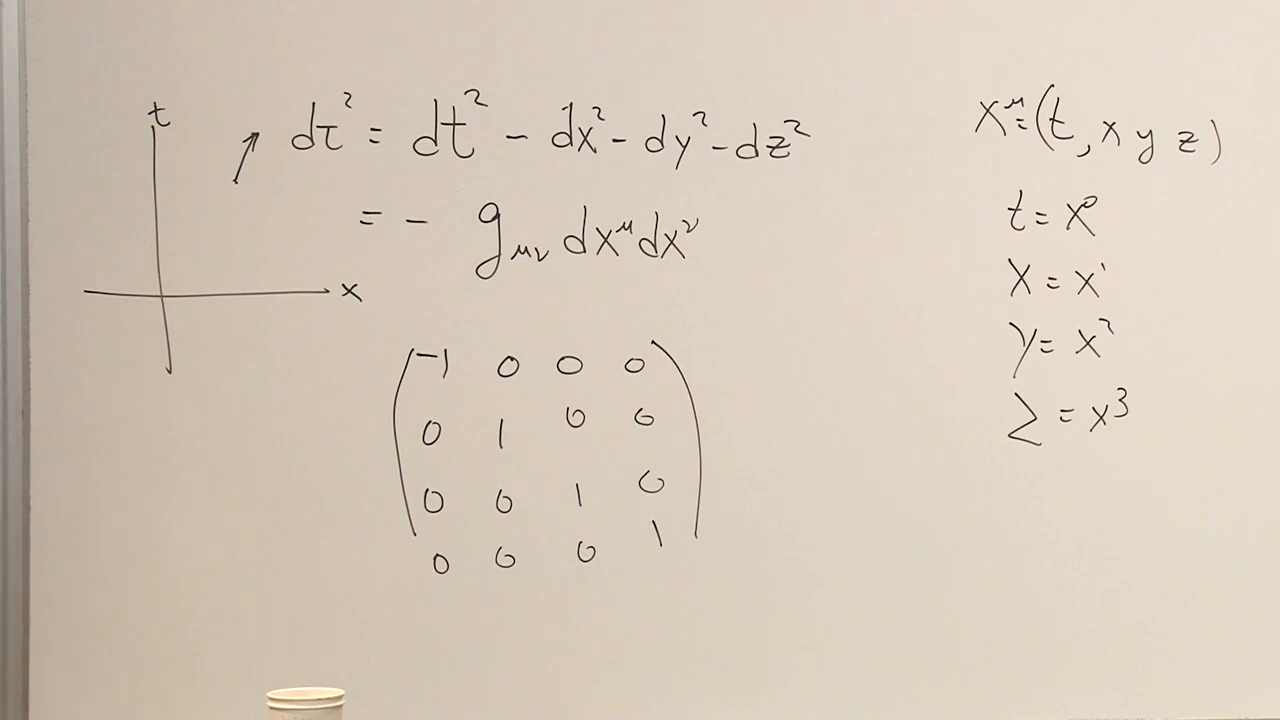
\includegraphics[width=0.92\textwidth]{lecture_04_figure_04.png}
\caption{La variation ordinaire des composantes et la correction de connexion le long d’une courbe.}
\end{figure}

Le vecteur est transporté parallèlement lorsque cette variation covariante s’annule :
\begin{equation}
\boxed{
dV^n+\Gamma^n{}_{mr}V^r\,dx^m=0.
}
\label{eq:l4-parallel-transport}
\end{equation}
Concrètement, on peut imaginer construire un repère normal en chaque point de la courbe. Dans ce repère local, le vecteur transporté ne doit pas tourner. On avance ensuite d’une distance infinitésimale, on construit le repère normal suivant et on recommence.

\begin{figure}[htbp]
\centering
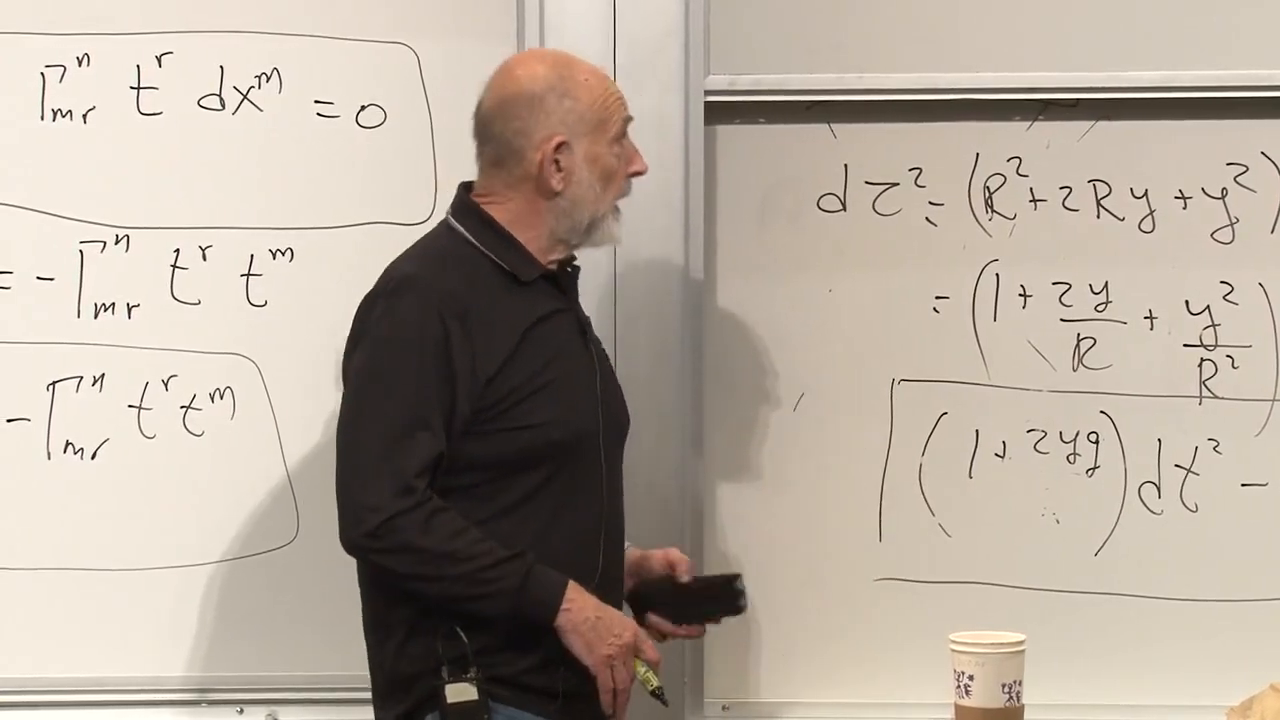
\includegraphics[width=0.92\textwidth]{lecture_04_figure_05.png}
\caption{Écriture claire de l’équation du transport parallèle au tableau.}
\end{figure}

L’orientation de chaque repère normal temporaire ne fait pas partie de la physique. On pourrait le faire tourner avant d’effectuer la comparaison. Ce qui compte, c’est que l’énoncé covariant \eqref{eq:l4-parallel-transport} soit indépendant de ce choix arbitraire.

\subsection{Dépendance au chemin et courbure}

Dans un espace courbe, le transport parallèle dépend du chemin. Partons du même vecteur au même point initial et transportons-le jusqu’au même point final en suivant deux chemins différents. En général, les vecteurs finaux diffèrent. Un vecteur transporté le long d’une boucle fermée peut revenir tourné. Cette différence est l’holonomie et constitue un signe direct de courbure.

\begin{figure}[htbp]
\centering
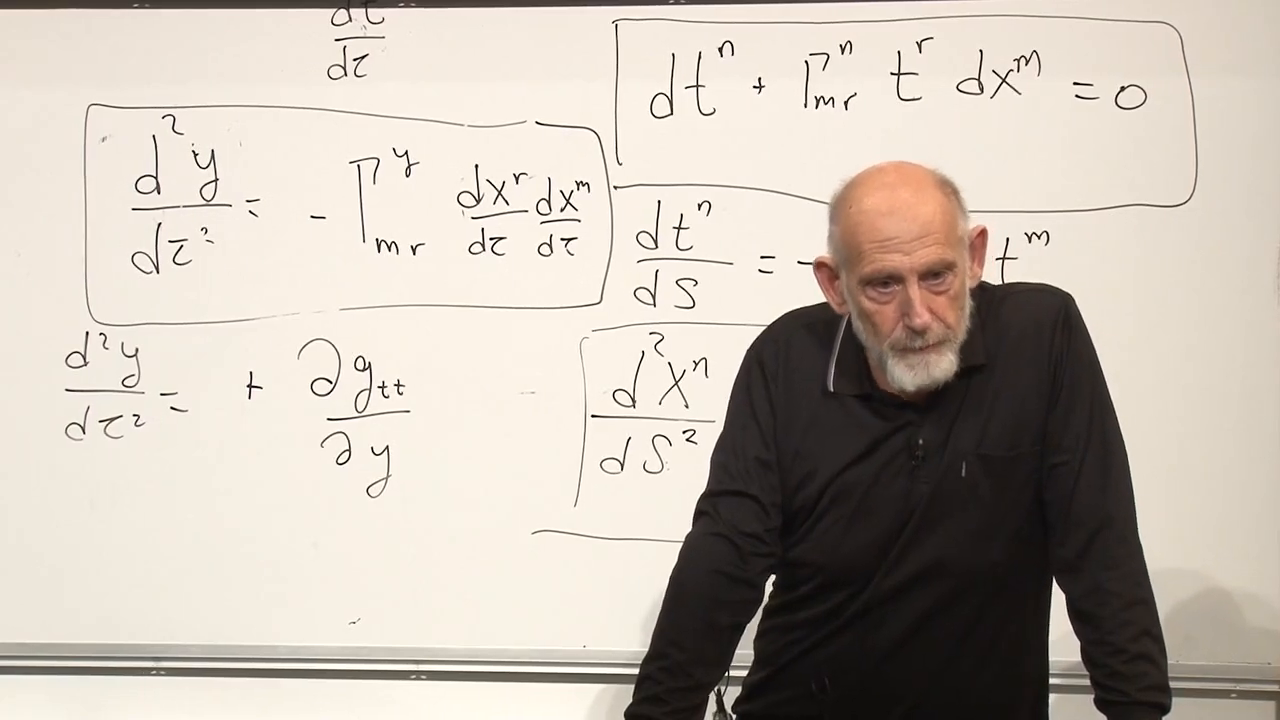
\includegraphics[width=0.90\textwidth]{lecture_04_figure_06.png}
\caption{Sur une surface courbe, deux chemins ne transportent pas nécessairement un vecteur selon la même orientation finale.}
\end{figure}

Le cône fournit un exemple utile. À l’écart de sa pointe, on peut découper un cône et l’aplatir. Pourtant, après le transport parallèle le long d’une boucle qui entoure la pointe, le vecteur revient tourné de l’angle de défaut. Si la pointe est arrondie, la courbure est finie et répartie sur une petite région. Si elle est parfaitement aiguë, l’idéalisation concentre la courbure en ce point.

\begin{figure}[htbp]
\centering
\includegraphics[width=0.90\textwidth]{lecture_04_figure_07.png}
\caption{Mouvement circulaire sur le cône et représentation plane après découpe.}
\end{figure}

\subsection{Questions sur le vecteur transporté}

\paragraph{Le vecteur doit-il être défini partout ?}
Non. On peut partir d’un seul vecteur en un point et résoudre \eqref{eq:l4-parallel-transport} uniquement le long de la courbe choisie. Un champ vectoriel complet est facultatif. Si un champ est défini sur une région, il peut être covariantement constant dans une direction et ne pas l’être dans une autre.

\paragraph{Sa norme est-elle conservée ?}
Oui. Posons \(V^2=g_{mn}V^mV^n\). Le long de la courbe,
\begin{align}
\frac{D}{d\lambda}\left(g_{mn}V^mV^n\right)
&=
\frac{Dg_{mn}}{d\lambda}V^mV^n
+2g_{mn}V^m\frac{DV^n}{d\lambda}\\
&=0.
\end{align}
La compatibilité métrique annule le premier terme et le transport parallèle annule le second. Les normes et les angles mutuels des vecteurs transportés parallèlement sont donc conservés.

\paragraph{Le vecteur tangent à toute courbe est-il transporté parallèlement ?}
Non. Cette question mène directement aux géodésiques. Le vecteur tangent à un chemin circulaire autour d’un cône tourne continuellement. Celui de la droite obtenue en découpant le cône ne tourne pas. Seul le second chemin est localement rectiligne.

\section{Géodésiques : le chemin le plus droit, pas seulement le plus court}

Une géodésique admet deux descriptions liées. Globalement, c’est un chemin stationnaire pour la fonctionnelle de longueur ou de temps propre. Localement, c’est le chemin le plus droit possible. Le mot « stationnaire » est important : selon la géométrie et les extrémités considérées, le chemin n’est pas forcément l’unique minimum global. Dans l’espace-temps lorentzien, les géodésiques de genre temps maximisent localement le temps propre plutôt que de minimiser une distance positive.

C’est la description locale qui nous est utile ici. Une petite voiture roulant sur un terrain courbe, avec le volant maintenu droit devant, suit une géodésique, à condition que sa taille soit petite devant l’échelle à laquelle le terrain se courbe. Sa trajectoire n’a pas besoin de paraître droite dans un espace ambiant : elle est droite selon la géométrie définie sur la surface.

\begin{figure}[htbp]
\centering
\includegraphics[width=0.90\textwidth]{lecture_04_figure_08.png}
\caption{Trajectoire tracée intrinsèquement sur la surface courbe, pour introduire la définition du chemin le plus droit.}
\end{figure}

\subsection{Le vecteur tangent}

Soit la courbe \(x^m(s)\), de longueur d’arc
\begin{equation}
ds^2=g_{mn}\,dx^m dx^n.
\end{equation}
Son vecteur tangent unitaire est
\begin{equation}
t^m=\frac{dx^m}{ds}.
\label{eq:l4-unit-tangent}
\end{equation}
Géométriquement, prenons deux points voisins, formons le vecteur déplacement qui les relie, divisons-le par leur distance, puis faisons coïncider les deux points.

\begin{figure}[htbp]
\centering
\includegraphics[width=0.90\textwidth]{lecture_04_figure_09.png}
\caption{La direction tangente comme limite du déplacement le long d’une courbe.}
\end{figure}

\begin{figure}[htbp]
\centering
\includegraphics[width=0.90\textwidth]{lecture_04_figure_10.png}
\caption{Élément de ligne et vecteur tangent unitaire \(t^m=dx^m/ds\).}
\end{figure}

Une géodésique est une courbe dont le vecteur tangent est transporté parallèlement le long de la courbe elle-même :
\begin{equation}
dt^n+\Gamma^n{}_{mr}t^r\,dx^m=0.
\end{equation}
Divisons par \(ds\) et utilisons \(dx^m/ds=t^m\) :
\begin{equation}
\frac{dt^n}{ds}
=
-\Gamma^n{}_{mr}t^m t^r.
\end{equation}
Enfin, substituons \(t^n=dx^n/ds\) :
\begin{equation}
\boxed{
\frac{d^2x^n}{ds^2}
+\Gamma^n{}_{mr}
\frac{dx^m}{ds}
\frac{dx^r}{ds}
=0.
}
\label{eq:l4-geodesic}
\end{equation}

\begin{figure}[htbp]
\centering
\includegraphics[width=0.94\textwidth]{lecture_04_figure_11.png}
\caption{Loi de transport du vecteur tangent et équation géodésique du second ordre.}
\end{figure}

L’équation \eqref{eq:l4-geodesic} ressemble déjà à la dynamique newtonienne. Si l’on remplace \(s\) par un paramètre de temps approprié, le premier terme est une accélération. Le terme de connexion joue alors le rôle d’une force par unité de masse, entièrement déterminée par la métrique. En relativité générale, cette analogie devient littérale : les particules libres suivent des géodésiques de l’espace-temps, et ce que Newton appelait l’accélération gravitationnelle apparaît par l’intermédiaire de la connexion.

\section{De la distance riemannienne au temps propre de l’espace-temps}

La discussion passe maintenant de l’espace courbe à l’espace-temps. Dans des coordonnées cartésiennes inertielles, le temps propre entre des événements voisins est
\begin{equation}
d\tau^2
=dt^2-dx^2-dy^2-dz^2.
\label{eq:l4-proper-time}
\end{equation}
Le cours utilise
\begin{equation}
d\tau^2=-g_{\mu\nu}\,dx^\mu dx^\nu
\label{eq:l4-lecture-sign}
\end{equation}
avec
\begin{equation}
g_{\mu\nu}
=
\eta_{\mu\nu}
=
\begin{pmatrix}
-1&0&0&0\\
0&1&0&0\\
0&0&1&0\\
0&0&0&1
\end{pmatrix}.
\label{eq:l4-eta}
\end{equation}
Le signe moins extérieur dans \eqref{eq:l4-lecture-sign} convertit donc la métrique choisie, de signature principalement positive, en \eqref{eq:l4-proper-time}. Les coordonnées sont
\begin{equation}
\begin{aligned}
x^\mu&=(t,x,y,z),\\
x^0&=t,\quad x^1=x,\\
x^2&=y,\quad x^3=z.
\end{aligned}
\end{equation}

\begin{figure}[htbp]
\centering
\includegraphics[width=0.94\textwidth]{lecture_04_figure_12.png}
\caption{Temps propre, coordonnées de l’espace-temps et métrique de Minkowski à signature principalement positive.}
\end{figure}

L’information invariante est la signature : une valeur propre a le signe associé au temps et trois ont celui associé à l’espace. Multiplier la métrique entière par \(-1\) et ajuster toutes les conventions de façon cohérente donne la convention tout aussi courante à signature principalement négative. Aucun phénomène physique ne dépend de ce choix global.

Le cours demande si l’on a envisagé des espaces ayant d’autres signatures indéfinies. Mathématiquement, les géométries pseudo-riemanniennes de nombreuses signatures sont bien établies. Le point physique est plus restreint : l’espace-temps relativiste observé est lorentzien, avec une direction temporelle. Des directions temporelles supplémentaires modifieraient profondément la structure causale et ne décrivent pas la physique examinée ici.

\begin{figure}[htbp]
\centering
\includegraphics[width=0.94\textwidth]{lecture_04_figure_13.png}
\caption{La convention de signe est vérifiée avant que la métrique plate soit notée \(\eta_{\mu\nu}\).}
\end{figure}

Un espace-temps plat n’exige pas que les composantes de la métrique aient l’allure de \(\eta_{\mu\nu}\) dans tous les systèmes de coordonnées. Cela signifie qu’il existe des coordonnées dans lesquelles elles l’ont. Des coordonnées curvilignes ou accélérées peuvent faire varier les composantes avec la position, même si le tenseur de Riemann est nul.

\section{Pourquoi une même accélération des coordonnées ne donne pas un système rigide}

Nous voulons construire des coordonnées liées à un ascenseur en accélération. La première idée consiste à aligner plusieurs observateurs à des distances fixes et à leur donner à tous la même accélération coordonnée. La relativité empêche cette construction naïve de rester rigide.

\begin{figure}[htbp]
\centering
\includegraphics[width=0.92\textwidth]{lecture_04_figure_14.png}
\caption{Alignement d’observateurs voisins pour vérifier si une accélération commune préserve la rigidité.}
\end{figure}

Si, dans un même repère inertiel, des observateurs séparés suivent des programmes d’accélération identiques, leur distance ne reste pas fixe dans leurs repères de repos instantanés changeants. Une corde qui les relie s’étire et finit par rompre. C’est la même tension cinématique que celle mise en évidence par l’expérience de pensée des vaisseaux de Bell. De plus, une accélération coordonnée newtonienne constante ne peut se poursuivre indéfiniment : elle finirait par prédire une vitesse supérieure à celle de la lumière.

Un repère accéléré rigide au sens relativiste doit donc appliquer une accélération propre différente à chaque position. Les observateurs plus proches de l’horizon auquel on s’approche accélèrent davantage ; ceux qui en sont plus éloignés accélèrent moins. Leurs distances propres peuvent alors rester constantes dans le repère comobile à l’instant considéré. Il s’agit d’une accélération rigide au sens de Born dans une dimension spatiale.

\section{Les coordonnées polaires euclidiennes : un préalable}

La construction correcte apparaît plus facilement si l’on commence par un cercle ordinaire. Dans un plan euclidien,
\begin{equation}
x=r\cos\theta,
\qquad
y=r\sin\theta,
\end{equation}
d’où
\begin{equation}
x^2+y^2=r^2,
\qquad
\cos^2\theta+\sin^2\theta=1.
\end{equation}
Les expressions faisant intervenir l’exponentielle complexe sont
\begin{equation}
\cos\theta=\frac{e^{i\theta}+e^{-i\theta}}{2},
\qquad
\sin\theta=\frac{e^{i\theta}-e^{-i\theta}}{2i}.
\label{eq:l4-euler-trig}
\end{equation}
Lors de la discussion au tableau, on remarque qu’il manque le facteur \(i\) au dénominateur de la formule du sinus, puis on le rétablit.

\begin{figure}[htbp]
\centering
\includegraphics[width=0.94\textwidth]{lecture_04_figure_15.png}
\caption{Cercle, coordonnées polaires euclidiennes et formes exponentielles des fonctions trigonométriques.}
\end{figure}

Une valeur fixe de \(r\) définit un cercle. Un mouvement à vitesse angulaire constante a une accélération centripète de norme constante, toujours dirigée vers l’intérieur. L’hyperbole jouera le rôle correspondant dans l’espace-temps.

\section{Coordonnées hyperboliques dans l’espace-temps de Minkowski}

Remplaçons les fonctions trigonométriques par leurs analogues hyperboliques :
\begin{equation}
\cosh\omega=\frac{e^\omega+e^{-\omega}}{2},
\qquad
\sinh\omega=\frac{e^\omega-e^{-\omega}}{2},
\end{equation}
avec
\begin{equation}
\cosh^2\omega-\sinh^2\omega=1.
\label{eq:l4-hyperbolic-identity}
\end{equation}
Il n’y a pas de facteur \(i\). La coordonnée \(\omega\) est un angle hyperbolique, ou rapidité. Contrairement à un angle ordinaire, elle n’est pas périodique ; elle varie de \(-\infty\) à \(+\infty\).

\begin{figure}[htbp]
\centering
\includegraphics[width=0.94\textwidth]{lecture_04_figure_16.png}
\caption{Dans la construction de l’espace-temps, les fonctions circulaires sont remplacées par les fonctions hyperboliques.}
\end{figure}

Définissons de nouvelles coordonnées dans le secteur de Rindler droit :
\begin{equation}
x=r\cosh\omega,
\qquad
t=r\sinh\omega,
\qquad
r>0.
\label{eq:l4-rindler-transform}
\end{equation}
Alors
\begin{equation}
x^2-t^2=r^2.
\label{eq:l4-rindler-hyperbola}
\end{equation}
À \(r\) fixe, la variation de \(\omega\) décrit une hyperbole. Faire croître \(r\) déplace d’une hyperbole à l’autre dans une direction de genre espace, tandis que faire croître \(\omega\) fait avancer le long d’une hyperbole, dans une direction de genre temps.

\begin{figure}[htbp]
\centering
\includegraphics[width=0.94\textwidth]{lecture_04_figure_17.png}
\caption{Transformation de coordonnées \(x=r\cosh\omega\), \(t=r\sinh\omega\) et hyperbole invariante correspondante.}
\end{figure}

\begin{figure}[htbp]
\centering
\includegraphics[width=0.94\textwidth]{lecture_04_figure_18.png}
\caption{Famille d’hyperboles à \(r\) fixe représentant un ensemble d’observateurs en accélération rigide.}
\end{figure}

\subsection{La métrique en coordonnées accélérées}

Dérivons \eqref{eq:l4-rindler-transform} :
\begin{align}
dx&=\cosh\omega\,dr+r\sinh\omega\,d\omega,\\
dt&=\sinh\omega\,dr+r\cosh\omega\,d\omega.
\end{align}
En utilisant \eqref{eq:l4-hyperbolic-identity}, les termes croisés s’annulent :
\begin{align}
d\tau^2
&=dt^2-dx^2\\
&=r^2\,d\omega^2-dr^2.
\label{eq:l4-rindler-metric}
\end{align}
Une fois les directions transversales rétablies, elles ajoutent simplement \(-dy^2-dz^2\) à la convention de temps propre utilisée ici.

Il s’agit toujours d’un espace-temps plat. Le coefficient dépendant des coordonnées \(r^2\) n’indique pas plus une courbure que le facteur \(r^2\) devant \(d\theta^2\) dans les coordonnées polaires euclidiennes.

\subsection{Accélération propre le long des hyperboles}

Pour une ligne d’univers fixe \(r=R\), l’équation \eqref{eq:l4-rindler-metric} donne
\begin{equation}
d\tau=R\,d\omega.
\end{equation}
Sa quadrivitesse est
\begin{equation}
U^\mu
=
\frac{d(t,x)}{d\tau}
=
(\cosh\omega,\sinh\omega),
\end{equation}
et sa quadriaccélération est
\begin{equation}
A^\mu
=
\frac{dU^\mu}{d\tau}
=
\frac{1}{R}(\sinh\omega,\cosh\omega).
\end{equation}
Sa norme invariante est constante :
\begin{equation}
a=\sqrt{A^\mu A_\mu}=\frac{1}{R}
\qquad (c=1).
\label{eq:l4-proper-acceleration}
\end{equation}

\begin{figure}[htbp]
\centering
\includegraphics[width=0.90\textwidth]{lecture_04_figure_19.png}
\caption{Loi en raison inverse \(a=1/R\) pour une ligne d’univers accélérée fixe.}
\end{figure}

En rétablissant les unités,
\begin{equation}
\boxed{a=\frac{c^2}{R}.}
\label{eq:l4-proper-acceleration-units}
\end{equation}

\begin{figure}[htbp]
\centering
\includegraphics[width=0.90\textwidth]{lecture_04_figure_20.png}
\caption{Le rétablissement des unités transforme \(1/R\) en \(c^2/R\).}
\end{figure}

Plus l’interception \(R\) est petite, plus la ligne d’univers se courbe fortement et plus l’accélération propre ressentie par l’observateur est grande. Les hyperboles plus éloignées se courbent moins et exigent une accélération plus faible. Chaque observateur a une accélération constante au cours du temps, mais les accélérations diffèrent d’un observateur à l’autre. C’est précisément cette variation qui préserve les distances propres entre eux.

\subsection{Questions sur les coordonnées accélérées}

\paragraph{\(R\) est-il l’intercept selon \(x\) ?}
Oui. Pour \(\omega=0\), l’équation \eqref{eq:l4-rindler-transform} donne \(t=0\) et \(x=R\). L’intercept détermine l’accélération propre par \eqref{eq:l4-proper-acceleration-units}.

\paragraph{La construction dépend-elle de l’origine choisie ?}
Les coordonnées en dépendent. Une translation de l’origine produit une autre famille d’hyperboles, dont les asymptotes sont déplacées. Aucun phénomène physique invariant ne dépend de ce choix. Nous sélectionnons délibérément un système de coordonnées accéléré et cherchons à savoir comment le mouvement inertiel s’y décrit.

\paragraph{Qu’est-ce que l’accélération propre ?}
C’est l’accélération mesurée par un accéléromètre solidaire de l’observateur. Covariamment,
\begin{equation}
A^\mu=\frac{dU^\mu}{d\tau},
\qquad
U^\mu=\frac{dx^\mu}{d\tau}.
\end{equation}
Sa norme est la poussée effectivement ressentie par l’observateur, et non l’accélération coordonnée \(d^2x/dt^2\) attribuée par un repère distant.

\section{Métriques plates en coordonnées polaires et hyperboliques}

Avant de nous placer au voisinage de la Terre, il est utile de mettre côte à côte les métriques euclidienne et lorentzienne. Dans le plan,
\begin{equation}
ds^2=dr^2+r^2d\theta^2,
\qquad
g_{ab}
=
\begin{pmatrix}
1&0\\
0&r^2
\end{pmatrix}.
\label{eq:l4-polar-metric}
\end{equation}
Une suggestion de l’auditoire introduit brièvement un facteur sphérique, mais il s’agit d’un plan, pas d’une sphère. Le terme \(r^2\) traduit le fait qu’un intervalle angulaire donné couvre un arc plus long à plus grand rayon.

\begin{figure}[htbp]
\centering
\includegraphics[width=0.94\textwidth]{lecture_04_figure_21.png}
\caption{Métrique polaire euclidienne : composantes dépendant de la position dans un plan plat.}
\end{figure}

L’analogue de Minkowski est
\begin{equation}
d\tau^2=r^2d\omega^2-dr^2.
\end{equation}
Les deux métriques ont des composantes qui dépendent de la position, alors que les deux géométries sont plates. La courbure des coordonnées et la courbure géométrique sont deux choses différentes.

\section{Localisation au voisinage de l’accélération terrestre}

Choisissons une hyperbole de référence dont l’accélération propre est égale à la valeur terrestre \(g\) :
\begin{equation}
g=\frac{c^2}{R},
\qquad
R=\frac{c^2}{g}.
\label{eq:l4-earth-radius}
\end{equation}

\begin{figure}[htbp]
\centering
\includegraphics[width=0.94\textwidth]{lecture_04_figure_22.png}
\caption{Choix de l’hyperbole de référence au moyen de \(c^2/R=g\).}
\end{figure}

Numériquement,
\begin{equation}
R
\simeq
\frac{(3.0\times10^8\ {\rm m\,s^{-1}})^2}
{9.8\ {\rm m\,s^{-2}}}
\simeq
9.2\times10^{15}\ {\rm m}.
\end{equation}
Le cours arrondit cette valeur à \(10^{16}\) mètres. Un champ d’un \(g\) terrestre est modeste à l’échelle relativiste ; le rayon de Rindler correspondant est donc immense.

Examinons maintenant un petit voisinage seulement de cet observateur de référence. Introduisons une hauteur locale \(y\) définie par
\begin{equation}
r=R+y,
\qquad
dr=dy,
\qquad
|y|\ll R.
\label{eq:l4-local-height}
\end{equation}
L’égalité \(dr=dy\) est explicitement repérée pendant la discussion ; le terme spatial doit donc s’écrire \(-dy^2\).

La substitution dans \eqref{eq:l4-rindler-metric} donne
\begin{align}
d\tau^2
&=(R+y)^2d\omega^2-dy^2\\
&=(R^2+2Ry+y^2)d\omega^2-dy^2\\
&=
\left(
1+\frac{2y}{R}+\frac{y^2}{R^2}
\right)
R^2d\omega^2-dy^2.
\label{eq:l4-local-expand}
\end{align}

\begin{figure}[htbp]
\centering
\includegraphics[width=0.94\textwidth]{lecture_04_figure_23.png}
\caption{Développement de la métrique accélérée au voisinage de \(r=R+y\).}
\end{figure}

Définissons une coordonnée de temps local
\begin{equation}
t=R\omega.
\label{eq:l4-local-time}
\end{equation}
Alors
\begin{equation}
d\tau^2
=
\left(
1+\frac{2y}{R}+\frac{y^2}{R^2}
\right)dt^2-dy^2.
\label{eq:l4-local-exact}
\end{equation}

\begin{figure}[htbp]
\centering
\includegraphics[width=0.94\textwidth]{lecture_04_figure_24.png}
\caption{Introduction de \(t=R\omega\) après le développement autour de l’hyperbole de référence.}
\end{figure}

Même un déplacement vertical de plusieurs dizaines de kilomètres est minuscule devant \(R\). Pour rendre la comparaison parlante, le cours considère une chute d’environ vingt-quatre miles : cette distance reste négligeable devant \(10^{16}\) mètres. Par conséquent, \(y^2/R^2\) est beaucoup plus petit que \(y/R\), et l’on peut négliger le terme quadratique :
\begin{equation}
d\tau^2
\simeq
\left(1+\frac{2y}{R}\right)dt^2-dy^2.
\label{eq:l4-local-linear}
\end{equation}

\begin{figure}[htbp]
\centering
\includegraphics[width=0.94\textwidth]{lecture_04_figure_25.png}
\caption{Métrique développée et changement de variable pour le temps local avant la troncature en champ faible.}
\end{figure}

Dans les unités où \(c=1\), l’équation \eqref{eq:l4-earth-radius} donne \(1/R=g\), et donc
\begin{equation}
\boxed{
d\tau^2\simeq(1+2gy)\,dt^2-dy^2.
}
\label{eq:l4-uniform-metric}
\end{equation}

\begin{figure}[htbp]
\centering
\includegraphics[width=0.94\textwidth]{lecture_04_figure_26.png}
\caption{Métrique locale complète de l’ascenseur en accélération uniforme.}
\end{figure}

La quantité
\begin{equation}
\Phi(y)=gy
\end{equation}
est le potentiel gravitationnel newtonien par unité de masse dans un champ uniforme. Ainsi,
\begin{equation}
d\tau^2\simeq(1+2\Phi)\,dt^2-dy^2
\qquad (c=1).
\label{eq:l4-weak-potential-propertime}
\end{equation}
Avec la convention du cours \(d\tau^2=-g_{\mu\nu}dx^\mu dx^\nu\), cela signifie que
\begin{equation}
g_{tt}=-(1+2\Phi).
\label{eq:l4-gtt-potential}
\end{equation}
En unités conventionnelles, la correction sans dimension est \(2\Phi/c^2\).

L’espace-temps n’a subi aucune courbure. L’équation \eqref{eq:l4-uniform-metric} est le développement local d’une métrique plate de Rindler. La gravité apparente est la force d’inertie ressentie dans un ascenseur accéléré.

\section{L’équation géodésique devient la loi de Newton}

Jusqu’ici, l’identification de \(gy\) à un potentiel n’était qu’une suggestion. Le test décisif est dynamique : une particule libre dans la métrique \eqref{eq:l4-uniform-metric} accélère-t-elle vers le bas avec \(d^2y/dt^2=-g\) ?

Pour une ligne d’univers de genre temps paramétrée par le temps propre,
\begin{equation}
\frac{d^2x^\nu}{d\tau^2}
+\Gamma^\nu{}_{\mu\rho}
\frac{dx^\mu}{d\tau}
\frac{dx^\rho}{d\tau}
=0.
\label{eq:l4-spacetime-geodesic}
\end{equation}
La composante verticale est
\begin{equation}
\frac{d^2y}{d\tau^2}
=
-\Gamma^y{}_{\mu\rho}
\frac{dx^\mu}{d\tau}
\frac{dx^\rho}{d\tau}.
\label{eq:l4-y-geodesic}
\end{equation}

\begin{figure}[htbp]
\centering
\includegraphics[width=0.94\textwidth]{lecture_04_figure_27.png}
\caption{Équation de transport et sa forme géodésique du second ordre, prêtes à être appliquées au mouvement vertical.}
\end{figure}

\subsection{Approximation des faibles vitesses}

Pour une particule se déplaçant lentement dans un champ faible et statique,
\begin{equation}
\frac{dt}{d\tau}\simeq1,
\qquad
\left|\frac{dy}{d\tau}\right|\ll1.
\end{equation}
La composante temporelle de la quadrivitesse est donc de l’ordre de l’unité, tandis que les composantes spatiales sont petites devant elle. Parmi les produits de \eqref{eq:l4-y-geodesic}, le terme dominant correspond à \(\mu=\rho=t\) :
\begin{equation}
\frac{d^2y}{d\tau^2}
\simeq
-\Gamma^y{}_{tt}
\left(\frac{dt}{d\tau}\right)^2
\simeq
-\Gamma^y{}_{tt}.
\label{eq:l4-slow-geodesic}
\end{equation}

\begin{figure}[htbp]
\centering
\includegraphics[width=0.94\textwidth]{lecture_04_figure_28.png}
\caption{Spécialisation de l’équation géodésique de l’espace-temps à la composante \(y\) pour un mouvement lent.}
\end{figure}

Calculons maintenant le seul coefficient de connexion nécessaire. La métrique est diagonale et indépendante de \(t\), donc
\begin{align}
\Gamma^y{}_{tt}
&=
\frac{1}{2}g^{yy}
\left(
\partial_tg_{yt}
+\partial_tg_{ty}
-\partial_yg_{tt}
\right)\\
&=
-\frac{1}{2}\partial_yg_{tt},
\label{eq:l4-gamma-ytt}
\end{align}
car \(g^{yy}=1\) dans la convention tensorielle à signature principalement positive du cours.

\begin{figure}[htbp]
\centering
\includegraphics[width=0.94\textwidth]{lecture_04_figure_29.png}
\caption{Formule de Christoffel réduite à la composante \(y,t,t\).}
\end{figure}

En combinant \eqref{eq:l4-slow-geodesic} et \eqref{eq:l4-gamma-ytt},
\begin{equation}
\frac{d^2y}{d\tau^2}
\simeq
\frac{1}{2}\partial_yg_{tt}.
\label{eq:l4-accel-gtt}
\end{equation}
D’après \eqref{eq:l4-gtt-potential},
\begin{equation}
\partial_yg_{tt}
=
-2\partial_y\Phi
=
-2g.
\end{equation}
Par conséquent,
\begin{equation}
\boxed{
\frac{d^2y}{d\tau^2}=-g.
}
\label{eq:l4-newton-result}
\end{equation}
Comme \(t\simeq\tau\) dans la même approximation de faible vitesse, on obtient aussi
\begin{equation}
\frac{d^2y}{dt^2}=-g.
\end{equation}

\begin{figure}[htbp]
\centering
\includegraphics[width=0.94\textwidth]{lecture_04_figure_30.png}
\caption{Enchaînement complet des signes : la dérivée par rapport à \(y\) de \(g_{tt}\) donne l’accélération \(-g\).}
\end{figure}

Plus généralement, dans le régime newtonien,
\begin{equation}
\boxed{
\begin{aligned}
g_{tt}&=-(1+2\Phi),\\
\frac{d^2x^i}{dt^2}&=-\partial_i\Phi
\end{aligned}
}
\qquad(c=1).
\label{eq:l4-newton-general}
\end{equation}
Lorsque les unités sont rétablies, la correction métrique est \(2\Phi/c^2\), tandis que l’accélération reste \(-\boldsymbol{\nabla}\Phi\).

Ce calcul explique pourquoi la métrique, plutôt qu’un champ de force gravitationnelle distinct, est l’objet central. Une particule libre suit simplement une géodésique de l’espace-temps. Dans des coordonnées adaptées à un laboratoire accéléré, cette géodésique présente la courbure coordonnée habituellement attribuée à la gravité.

\subsection{Question sur l’origine de Rindler choisie}

Aurait-on pu décaler l’hyperbole de référence, de sorte que ses asymptotes et son intercept se trouvent ailleurs ? Oui. Il existe un système de coordonnées à accélération uniforme associé à toute origine translatée adéquate. Dans l’image de l’ascenseur, ces choix reviennent à sélectionner des ascenseurs dont les planchers occupent des positions différentes à un instant donné.

Le résultat local ne repose pas sur une origine privilégiée. Une fois choisi un observateur de référence d’accélération \(g\), \(y\) mesure la hauteur par rapport à cet observateur et la métrique voisine prend la forme \eqref{eq:l4-uniform-metric}. Le choix arbitraire des coordonnées détermine où nous situons le plancher dans la description ; il ne crée pas de courbure invariante.

\section{Pourquoi le symbole de Christoffel ne peut pas être un tenseur}

La discussion après le cours revient sur un point apparu lors du rappel. Dans les coordonnées inertielles initiales,
\begin{equation}
g_{\mu\nu}=\eta_{\mu\nu},
\qquad
\partial_\rho\eta_{\mu\nu}=0,
\qquad
\Gamma^\mu{}_{\nu\rho}=0.
\end{equation}
Une particule libre suit une droite et aucune force gravitationnelle n’agit sur elle.

Dans les coordonnées accélérées, le même espace-temps plat possède des composantes métriques dépendant de la position. Ses symboles de Christoffel ne s’annulent pas et la même trajectoire inertielle paraît courbe. La particule semble tomber vers le plancher de l’ascenseur.

Cela serait impossible si \(\Gamma^\mu{}_{\nu\rho}\) était un tenseur. Un tenseur nul dans un repère est nul dans tous les repères. La connexion acquiert au contraire un terme inhomogène lors d’une transformation de coordonnées ; elle peut donc être nulle dans un repère inertiel et non nulle dans un repère accéléré. C’est exactement ce qu’exige le principe d’équivalence :
\begin{equation}
\text{accelerated frame}
\quad\longleftrightarrow\quad
\text{local gravity}.
\end{equation}

La courbure se comporte autrement. Le tenseur de Riemann est un tenseur. S’il s’annule dans le repère inertiel, il s’annule également dans le repère accéléré :
\begin{equation}
R^\mu{}_{\nu\rho\sigma}=0.
\end{equation}
Les symboles de Christoffel décrivent donc une force gravitationnelle dépendant des coordonnées, tandis que la courbure détecte le contenu de marée invariant qu’aucun changement de coordonnées ne peut éliminer.

\section{Du potentiel uniforme à un aperçu de Schwarzschild}

L’ascenseur accéléré ne contient aucune matière gravitationnelle et ne présente aucune courbure. Pourtant, la relation de champ faible \eqref{eq:l4-newton-general} suggère ce qu’il faut rechercher dans le champ d’une masse sphérique réelle. Le potentiel newtonien à l’extérieur d’une masse \(M\) est
\begin{equation}
\Phi(r)=-\frac{GM}{r}.
\label{eq:l4-newton-potential}
\end{equation}
En le substituant dans la composante temporelle de la métrique en champ faible, on obtient
\begin{equation}
g_{tt}
\simeq
-\left(1-\frac{2GM}{r}\right)
\qquad(c=1).
\label{eq:l4-schwarzschild-preview}
\end{equation}
Le signe du potentiel est corrigé lors de la discussion au tableau. Pour qu’il y ait attraction, le potentiel doit être négatif et tendre vers zéro par valeurs négatives lorsque \(r\) tend vers l’infini.

\begin{figure}[htbp]
\centering
\includegraphics[width=0.94\textwidth]{lecture_04_figure_31.png}
\caption{Potentiel newtonien introduit dans le coefficient temporel de la métrique, faisant apparaître le facteur \(1-2GM/r\).}
\end{figure}

Le coefficient s’annule pour
\begin{equation}
r=2GM
\qquad(c=1),
\end{equation}
ou, une fois les unités rétablies,
\begin{equation}
r_s=\frac{2GM}{c^2}.
\end{equation}
C’est le rayon de Schwarzschild. L’annulation de ce coefficient particulier de la métrique annonce la présence d’un horizon.

L'argument est délibérément présenté comme un aperçu, et non comme une dérivation. À elle seule, l'approximation de champ faible ne permet pas d'établir la solution exacte de Schwarzschild près de \(r=2GM/c^2\), précisément là où la correction cesse d'être petite. La solution complète comporte aussi une composante radiale non triviale et doit satisfaire les équations du champ d'Einstein. Ces équations n'ont pas encore été introduites. Le raisonnement présenté ici met en évidence l'indice structurel pertinent et l'échelle à laquelle doit apparaître un phénomène qualitativement nouveau.

\section{Questions et corrections en classe}

\subsection{Un angle hyperbolique se comporte-t-il comme un angle ordinaire ?}

Non. Les deux paramètres décrivent un mouvement le long d'une famille de courbes à rayon constant, mais \(\theta\) est périodique, tandis que la rapidité \(\omega\) varie sur toute la droite réelle. Le mot « angle » renvoie à l'analogie algébrique entre les rotations et les transformations de Lorentz, et non à une quantité limitée entre \(0\) et \(2\pi\).

\subsection{Pourquoi une accélération modeste exige-t-elle un R énorme ?}

La relation \(a=c^2/R\) fait intervenir la grande échelle relativiste \(c^2\). Pour obtenir seulement \(10\ {\rm m\,s^{-2}}\), il faut que \(R\) soit de l'ordre de \(10^{16}\) mètres. Il ne s'agit pas d'une nouvelle distance physique associée à la Terre, mais du rayon de courbure de la ligne d'univers hyperbolique dans un diagramme de Minkowski, exprimé en unités de longueur.

Ce grand rayon garantit aussi l'existence d'un intervalle où l'approximation newtonienne est utile. Aux échelles de temps et de distance d'un laboratoire, la vitesse reste très inférieure à \(c\), l'accélération varie de façon négligeable à l'échelle de l'appareillage et \(t\) diffère peu du temps propre.

\subsection{Le champ gravitationnel apparent est-il réel ?}

Il est réel en tant que lecture d'un accéléromètre pour un observateur maintenu à une position de Rindler fixe, mais il ne correspond pas à une courbure invariante. Si l'on libère l'observateur, l'accéléromètre indique zéro le long de la géodésique inertielle qui en résulte. Un laboratoire en chute libre suffisamment petit élimine localement le champ uniforme. En revanche, un champ de marée, représenté par une courbure non nulle, ne peut pas être éliminé sur une région de taille finie.

\subsection{Qu'a-t-on corrigé pendant le calcul de la force ?}

Plusieurs signes ainsi qu'un facteur égal à la moitié sont vérifiés en direct. Dans les conventions du cours, la chaîne fiable est
\begin{equation}
\begin{aligned}
g_{tt}&=-(1+2gy),\\
\Gamma^y{}_{tt}&=-\frac12\partial_yg_{tt}=g,\\
\frac{d^2y}{d\tau^2}&=-\Gamma^y{}_{tt}=-g.
\end{aligned}
\end{equation}
L'explicitation des conventions évite qu'une hésitation sur un signe au tableau ne devienne une ambiguïté physique.

\section{Ce qui a été établi}

Le cours commence par la géométrie différentielle et s'achève avec le corps en chute de Newton. Les étapes essentielles sont les suivantes :
\begin{enumerate}
\item Une dérivée covariante compare des tenseurs exprimés dans des bases de coordonnées qui varient.
\item Le transport parallèle correspond à une variation covariante nulle le long d'un chemin choisi.
\item Une géodésique transporte parallèlement son propre vecteur tangent.
\item Les particules libres suivent les géodésiques de l'espace-temps.
\item Les hyperboles de rayon fixe \(r\) forment un référentiel accéléré rigide au sens relativiste.
\item Leur accélération propre vaut \(a=c^2/r\) ; elle doit donc varier avec la position.
\item Au voisinage d'une ligne d'univers de référence d'accélération \(g\), la métrique plate s'écrit
\begin{equation}
d\tau^2\simeq(1+2gy)\,dt^2-dy^2
\qquad(c=1).
\end{equation}
\item Son équation géodésique se réduit à
\begin{equation}
\frac{d^2y}{dt^2}=-g.
\end{equation}
\end{enumerate}

Le principe d'équivalence n'est donc pas une simple analogie entre un ascenseur et la gravité. Il est encodé dans la manière dont la métrique et sa connexion se transforment. Une force gravitationnelle uniforme peut apparaître lorsque l'espace-temps plat est décrit dans des coordonnées accélérées, alors que la courbure reste nulle.

Cette extrapolation finale nous mène au-delà du champ uniforme. Remplacer \(\Phi=gy\) par \(\Phi=-GM/r\) prédit le facteur caractéristique \(1-2GM/r\) dans la composante temporelle d'une métrique sphérique et fait apparaître l'échelle de Schwarzschild. Pour déterminer la géométrie complète, il nous faut toutefois les équations du champ. C'est à cette tâche que sera consacré le prochain cours.

\graphicspath{{../../../generated_course_notes/core/general_relativity/2012_fall_theoretical_minimum/chapters/lecture_05/}{../../../generated_course_notes/core/general_relativity/2012_fall_theoretical_minimum/figures/}{../../../generated_course_notes/core/general_relativity/2012_fall_theoretical_minimum/assets/}}
\chapter{Cônes de lumière, géodésiques et horizon de Schwarzschild}

Le problème de l’horizon commence par une distinction déjà présente en relativité restreinte. Deux événements voisins peuvent être séparés selon une direction de genre temps, de genre espace ou de genre lumière. La courbure n’abolit pas cette classification. Elle fait du cône de lumière un objet local, différent en chaque événement, et rend la métrique elle-même dynamique. Une fois la métrique connue, le mouvement d’une particule en chute libre découle du même principe du temps propre qui décrit une particule relativiste libre dans un espace-temps plat.

Nous appliquerons ce principe à deux reprises. Il doit d’abord restituer le mouvement newtonien dans un champ faible. Nous l’appliquerons ensuite à la métrique de Schwarzschild, où la signification du temps, de la distance radiale et de la vitesse devient étonnamment subtile.

\section{Intervalles de genre temps, de genre espace et de genre lumière}

Dans un espace-temps plat, avec \(c=1\), l’élément de temps propre est
\begin{equation}
d\tau^2=dt^2-dx^2-dy^2-dz^2.
\label{eq:l5-minkowski-proper-time}
\end{equation}
Rétablir \(c\) est utile dès qu’une approximation non relativiste est proche :
\begin{equation}
d\tau^2
=dt^2-\frac{dx^2+dy^2+dz^2}{c^2}.
\label{eq:l5-minkowski-c}
\end{equation}
La notation \(d\tau^2\) ne garantit pas que le membre de droite soit positif. Son signe classe le déplacement :
\begin{align}
d\tau^2>0
&\quad\Longleftrightarrow\quad \text{time-like},\\
d\tau^2=0
&\quad\Longleftrightarrow\quad \text{light-like},\\
d\tau^2<0
&\quad\Longleftrightarrow\quad \text{space-like}.
\end{align}
Pour un déplacement de genre espace, il est commode de définir la distance propre positive
\begin{equation}
ds^2=-d\tau^2
=dx^2+dy^2+dz^2-dt^2
\qquad(c=1).
\label{eq:l5-proper-distance}
\end{equation}

Le cône de lumière organise ces trois possibilités. Sa surface, et non son intérieur, est constituée des directions de genre lumière. Les directions de genre temps se trouvent à l’intérieur du cône et celles de genre espace à l’extérieur. Les moitiés supérieure et inférieure représentent les cônes de lumière passé et futur.

\begin{figure}[htbp]
\centering
\includegraphics[width=0.82\textwidth]{lecture_05_figure_02.png}
\caption{Temps propre, distance propre et cône causal réunis au tableau. Les rayons lumineux se trouvent sur le cône lui-même ; son intérieur est de genre temps et son extérieur de genre espace.}
\lectureframe{00:05:44}
\end{figure}

\begin{figure}[htbp]
\centering
\begin{tikzpicture}[scale=1.0]
\draw[->] (0,-2.3) -- (0,2.3) node[above] {\(t\)};
\draw[->] (-2.4,0) -- (2.4,0) node[right] {\(x\)};
\draw (-1.6,1.6) -- (0,0) -- (1.6,1.6);
\draw (-1.6,-1.6) -- (0,0) -- (1.6,-1.6);
\fill (0,0) circle (1.4pt);
\draw[->,thick] (0,0) -- (0,1.2)
  node[midway,left] {\(\text{time-like}\)};
\draw[->,thick] (0,0) -- (1.7,0.35)
  node[midway,below] {\(\text{space-like}\)};
\node at (1.25,1.35) {\(\text{light-like}\)};
\end{tikzpicture}
\caption{Classification causale dans une section bidimensionnelle de l’espace-temps.}
\end{figure}

Ces intervalles sont opérationnels. Le temps propre est celui qu’indique une horloge transportée le long d’une ligne d’univers de genre temps. La distance propre est celle que mesure un ensemble approprié de règles graduées entre des événements séparés selon une direction de genre espace. Ce ne sont pas de simples noms donnés aux signes d’une forme quadratique.

\section{Signature lorentzienne et un cône en chaque événement}

Avec la convention tensorielle « surtout plus », la métrique plate a pour composantes
\begin{equation}
\eta_{\mu\nu}=\operatorname{diag}(-1,1,1,1),
\label{eq:l5-eta}
\end{equation}
et
\begin{equation}
d\tau^2=-\eta_{\mu\nu}\,dx^\mu dx^\nu.
\label{eq:l5-proper-time-eta}
\end{equation}
La matrice affichée est l’expression d’un tenseur de rang deux dans une base particulièrement simple. Sa caractéristique invariante est sa signature : une direction négative et trois directions positives,
\begin{equation}
\operatorname{signature}(\eta)=(-,+,+,+).
\label{eq:l5-lorentz-signature}
\end{equation}
Une métrique comportant deux signes négatifs aurait deux directions temporelles. De telles signatures peuvent être étudiées mathématiquement, mais elles ne décrivent pas l’espace-temps considéré ici.

Dans un espace-temps courbe, les composantes varient :
\begin{equation}
g_{\mu\nu}=g_{\mu\nu}(x).
\label{eq:l5-position-metric}
\end{equation}
En chaque événement, la métrique doit néanmoins conserver une signature lorentzienne. Chaque événement possède donc ses propres directions de genre temps, sa frontière de genre lumière et ses directions de genre espace. Dans un dessin en coordonnées, les cônes peuvent sembler inclinés ou aplatis différemment d’un point à l’autre, mais la classification causale demeure.

\begin{figure}[htbp]
\centering
\includegraphics[width=0.86\textwidth]{lecture_05_figure_03.png}
\caption{La métrique dépendant de la position \(g_{\mu\nu}(x)\), les étiquettes causales et des esquisses de cônes de lumière locaux.}
\lectureframe{00:09:41}
\end{figure}

\begin{figure}[htbp]
\centering
\begin{tikzpicture}[scale=1.0]
\draw[thick] (-4,-0.5) .. controls (-2,0.2) and (0,0.6) .. (3.5,0.1);
\foreach \x/\y/\a/\b in {-3/0/0.9/1.2, -0.6/0.35/0.55/1.25,
                          2.0/0.2/1.15/0.95} {
  \fill (\x,\y) circle (1.3pt);
  \draw (\x,\y) -- ++(-\a,1.2);
  \draw (\x,\y) -- ++(\a,1.2);
  \draw (\x,\y) -- ++(-\b,-1.2);
  \draw (\x,\y) -- ++(\b,-1.2);
}
\end{tikzpicture}
\caption{Cônes locaux voisins. Leur forme en coordonnées peut varier sans changer les vecteurs de genre temps, de genre lumière ou de genre espace.}
\end{figure}

\begin{classroomqa}
\audiencequestion{La valeur propre négative unique sélectionne-t-elle une direction temporelle unique ?}
\lecturerresponse{Une base qui diagonalise la matrice affichée possède une direction de base négative, mais cela ne sélectionne ni observateur privilégié ni flèche physique unique. Les transformations de Lorentz mélangent la coordonnée temporelle aux coordonnées spatiales, et tout vecteur situé à l’intérieur du cône est de genre temps. L’objet invariant est le cône associé à la signature une direction négative et trois positives, et non un vecteur de genre temps distingué.
\lecturetimestamp{00:12:17--00:17:24}}
\end{classroomqa}

\begin{classroomqa}
\audiencequestion{Pourquoi deux dessins du cône local peuvent-ils avoir des formes différentes ?}
\lecturerresponse{Les coordonnées peuvent modifier le dessin. Par exemple, remplacer \(x\) par une coordonnée redimensionnée modifie la pente numérique attribuée à un rayon lumineux et fait donc paraître le cône plus étroit ou plus large. Des coordonnées plus générales peuvent l’incliner. Il s’agit de représenter le même événement et les mêmes relations causales. Dans un espace-temps courbe, les cônes en des événements distincts appartiennent aussi à des espaces tangents distincts ; les comparer exige donc la métrique et une règle de transport.
\lecturetimestamp{00:13:37--00:15:59}}
\end{classroomqa}

\section{Les géodésiques comme problème variationnel}

Une particule libre suit une géodésique de l’espace-temps. Sous forme différentielle, avec un paramètre affine \(\lambda\),
\begin{equation}
\frac{d^2x^\mu}{d\lambda^2}
+\Gamma^\mu{}_{\rho\sigma}
\frac{dx^\rho}{d\lambda}
\frac{dx^\sigma}{d\lambda}=0.
\label{eq:l5-geodesic}
\end{equation}
La connexion indique au vecteur tangent comment rester parallèle à lui-même au cours du mouvement de la particule.

Il existe une deuxième formulation, souvent plus facile à utiliser pour les calculs. Dans un espace riemannien muni de la métrique \(g_{mn}\), la longueur d’une courbe est
\begin{equation}
s=\int ds
=\int\sqrt{g_{mn}\,dx^m dx^n}.
\label{eq:l5-spatial-length}
\end{equation}
La géodésique rend cette longueur stationnaire sous de petites variations du chemin à extrémités fixes. L’intégrale est simplement la somme des longueurs infinitésimales le long de la courbe, et son équation d’Euler--Lagrange est une équation différentielle du second ordre, analogue par sa forme à une loi de force.

Pour une ligne d’univers de genre temps, la longueur spatiale est remplacée par le temps propre :
\begin{equation}
\tau
=\int\sqrt{-g_{\mu\nu}\,dx^\mu dx^\nu}.
\label{eq:l5-proper-time-functional}
\end{equation}
Une géodésique de genre temps rend \(\tau\) stationnaire et, pour des trajectoires de chute libre voisines avant l’apparition de points conjugués, localement maximale. En multipliant par \(-m\), on obtient l’action de la particule
\begin{equation}
A=-m\tau
=-m\int\sqrt{-g_{\mu\nu}\,dx^\mu dx^\nu}.
\label{eq:l5-particle-action}
\end{equation}
Le même trajet minimise donc localement \(A=-m\tau\). La distinction entre un temps propre stationnaire et le signe de l’action choisie lève l’apparente ambiguïté entre minimum et maximum.

\section{Du temps propre au lagrangien usuel}

L’action de \eqref{eq:l5-particle-action} est géométrique, mais on peut la mettre sous la forme familière utilisée en mécanique. Paramétrons la ligne d’univers par la coordonnée \(t\), divisons chaque différentielle par \(dt\) et sortons de la racine le facteur restant \(dt\) :
\begin{align}
A
&=-m\int\sqrt{-g_{\mu\nu}(x)\,dx^\mu dx^\nu}\\
&=-m\int
\sqrt{-g_{\mu\nu}(x)
\frac{dx^\mu}{dt}\frac{dx^\nu}{dt}}\,dt.
\label{eq:l5-action-t}
\end{align}
Pour la composante temporelle, \(dt/dt=1\) ; les composantes spatiales sont les vitesses coordonnées usuelles. Nous pouvons donc écrire
\begin{equation}
\begin{aligned}
A&=\int L\,dt,\\
L&=-m\sqrt{-g_{\mu\nu}(x)\dot x^\mu\dot x^\nu},\\
\dot x^\mu&=\frac{dx^\mu}{dt}.
\end{aligned}
\label{eq:l5-relativistic-lagrangian}
\end{equation}

\begin{figure}[htbp]
\centering
\includegraphics[width=0.88\textwidth]{lecture_05_figure_05.png}
\caption{L’action de la ligne d’univers mise sous la forme usuelle \(A=\int L\,dt\).}
\lectureframe{00:27:00}
\end{figure}

\begin{figure}[htbp]
\centering
\includegraphics[width=0.88\textwidth]{lecture_05_figure_06.png}
\caption{Un état ultérieur du tableau où le lagrangien relativiste est isolé.}
\lectureframe{00:28:59}
\end{figure}

\begin{classroomqa}
\audiencequestion{Les indices d’espace-temps de cette action devraient-ils être grecs ?}
\lecturerresponse{Oui. Les indices grecs parcourent le temps et toutes les coordonnées spatiales. On peut réserver les indices latins aux coordonnées spatiales lorsque cette distinction est utile.
\lecturetimestamp{00:25:53--00:26:03}}
\end{classroomqa}

\begin{classroomqa}
\audiencequestion{Pourquoi appelle-t-on l’expression sous la racine le lagrangien ?}
\lecturerresponse{Une fois l’action écrite sous la forme \(A=\int L\,dt\), l’intégrande est le lagrangien. Ce n’est pas seulement une définition : la variation de cet intégrande donne les équations d’Euler--Lagrange
\[
\frac{d}{dt}
\left(\frac{\partial L}{\partial\dot x^\mu}\right)
=\frac{\partial L}{\partial x^\mu},
\]
qui sont équivalentes à l’équation des géodésiques, à condition de traiter la paramétrisation de façon cohérente.
\lecturetimestamp{00:28:36--00:29:02}}
\end{classroomqa}

Pour une particule massive, la ligne d’univers est de genre temps ; la quantité sous la racine est donc positive. Un trajet de genre espace décrirait un mouvement supraluminique, et non la trajectoire d’une particule massive ordinaire. Une fois la métrique connue, on peut obtenir la trajectoire de la particule soit en calculant les symboles de Christoffel et en utilisant \eqref{eq:l5-geodesic}, soit en appliquant les équations d’Euler--Lagrange à \eqref{eq:l5-relativistic-lagrangian}. Démontrer leur équivalence est un exercice utile ; la méthode de l’action est généralement plus courte.

\section{La limite newtonienne}

Considérons le champ gravitationnel faible et statique à l’extérieur d’une source sphérique. Partons de l’espace-temps plat et autorisons le coefficient de \(dt^2\) à différer légèrement de un :
\begin{equation}
d\tau^2
=\left(1+\frac{2u(\mathbf{x})}{c^2}\right)dt^2
-\frac{d\mathbf{x}^2}{c^2},
\label{eq:l5-weak-metric}
\end{equation}
où \(u\) doit devenir le potentiel newtonien. Cet ansatz doit être vérifié, et pas simplement nommé.

L’action de la particule, avec ses dimensions physiques, est
\begin{equation}
A=-mc^2\int
\sqrt{1+\frac{2u}{c^2}
-\frac{\dot{\mathbf{x}}^{\,2}}{c^2}}\,dt.
\label{eq:l5-weak-action}
\end{equation}
\(u/c^2\) et \(\dot{\mathbf{x}}^{\,2}/c^2\) sont tous deux petits. En conservant leurs contributions au premier ordre,
\begin{equation}
\sqrt{1+\epsilon}
=1+\frac{\epsilon}{2}+O(\epsilon^2),
\qquad
\epsilon=\frac{2u-\dot{\mathbf{x}}^{\,2}}{c^2},
\end{equation}
on obtient
\begin{align}
L
&=-mc^2
\sqrt{1+\frac{2u-\dot{\mathbf{x}}^{\,2}}{c^2}}\\
&=-mc^2-mu+\frac{m}{2}\dot{\mathbf{x}}^{\,2}\\
&\quad+O\!\left(c^{-2}
 [u^2+u\dot{\mathbf{x}}^{\,2}+\dot{\mathbf{x}}^{\,4}]\right).
\label{eq:l5-newton-expansion}
\end{align}
Le terme constant d’énergie de masse au repos n’a aucun effet sur les équations du mouvement. Il reste
\begin{equation}
L_{\mathrm{nr}}
=\frac{m}{2}\dot{\mathbf{x}}^{\,2}-m u(\mathbf{x}),
\label{eq:l5-newton-lagrangian}
\end{equation}
et, par conséquent,
\begin{equation}
m\ddot{\mathbf{x}}=-m\boldsymbol{\nabla}u.
\label{eq:l5-newton-equation}
\end{equation}
La masse d’épreuve se simplifie, comme l’exige la chute libre universelle. L’énergie potentielle est \(m u\), tandis que l’accélération est indépendante de \(m\).

Nous avons ainsi identifié la relation dominante en champ faible
\begin{equation}
g_{00}=1+\frac{2u}{c^2}+O(c^{-4}).
\label{eq:l5-g00-newton}
\end{equation}
À l’extérieur d’une masse sphérique \(M\),
\begin{equation}
u(r)=-\frac{GM}{r},
\qquad
g_{00}=1-\frac{2GM}{rc^2}+O(c^{-4}).
\label{eq:l5-g00-spherical}
\end{equation}
Cela détermine la première correction à la composante temporelle. Cela ne détermine pas encore la métrique complète en champ fort.

\section{Coordonnées sphériques et première conjecture de Schwarzschild}

Les coordonnées sphériques sont naturelles pour une source centrale. Dans le cours, \(\theta\) est mesuré depuis le plan équatorial plutôt que depuis le pôle ; l’élément de ligne angulaire est donc
\begin{equation}
d\Omega^2=d\theta^2+\cos^2\theta\,d\phi^2.
\label{eq:l5-angular-metric}
\end{equation}
Avec cette convention,
\begin{equation}
d\mathbf{x}^2=dr^2+r^2d\Omega^2.
\label{eq:l5-flat-spherical}
\end{equation}
Aucune grandeur physique ne dépend du choix de cette coordonnée \(\theta\), analogue à la latitude ; avec l’angle polaire plus courant, \(\cos^2\theta\) serait remplacé par \(\sin^2\theta\).

Insérer le coefficient temporel newtonien tout en laissant la métrique spatiale plate donne cette première conjecture :
\begin{equation}
\begin{aligned}
d\tau^2
&=\left(1-\frac{r_s}{r}\right)dt^2
-\frac{1}{c^2}\left(dr^2+r^2d\Omega^2\right),\\
r_s&=\frac{2GM}{c^2}.
\end{aligned}
\label{eq:l5-naive-schwarzschild}
\end{equation}
Ce ne peut pas être la réponse exacte. Pour \(r<r_s\), le coefficient de \(dt^2\) change de signe alors que tous les coefficients spatiaux restent négatifs dans la convention du temps propre. La métrique perdrait sa signature une direction temporelle et trois directions spatiales.

Les équations de champ dans le vide fournissent le coefficient radial requis :
\begin{equation}
\boxed{
d\tau^2
=\left(1-\frac{r_s}{r}\right)dt^2
-\frac{dr^2}{c^2\left(1-r_s/r\right)}
-\frac{r^2}{c^2}d\Omega^2.
}
\label{eq:l5-schwarzschild}
\end{equation}
C’est la métrique extérieure de Schwarzschild. Lorsque \(r\) franchit \(r_s\), les coefficients \(t\) et \(r\) changent de signe ensemble, préservant ainsi la signature lorentzienne. En coordonnées de Schwarzschild, la coordonnée radiale devient de genre temps à l’intérieur et la coordonnée \(t\) devient de genre espace. Cet échange signale une défaillance de la carte de coordonnées à l’horizon, et non une défaillance locale de la géométrie de l’espace-temps.

\begin{classroomqa}
\audiencequestion{Combien de temps un objet en chute met-il à franchir l’horizon ?}
\lecturerresponse{Selon la coordonnée de Schwarzschild \(t\) utilisée par un observateur lointain, le franchissement est repoussé à un temps infini. Selon le temps propre indiqué par l’horloge de l’objet en chute, il se produit en un temps fini. La distinction entre ces horloges est le problème central de l’horizon.
\lecturetimestamp{00:54:45--00:55:35}}
\end{classroomqa}

\begin{classroomqa}
\audiencequestion{Pourquoi modifier le coefficient radial plutôt qu’une autre partie de la métrique ?}
\lecturerresponse{La métrique doit conserver sa signature lorentzienne, la symétrie sphérique distingue la direction radiale de la sphère angulaire et les équations de champ dans le vide déterminent précisément le facteur réciproque. La signature indique où chercher ; les équations d’Einstein donnent le résultat exact.
\lecturetimestamp{00:55:35--00:56:01}}
\end{classroomqa}

Pour la Terre, \(r_s\) n’est que de l’ordre du centimètre, profondément enfoui dans le corps matériel. La métrique extérieure du vide n’y est pas valable ; la Terre n’a donc pas d’horizon de Schwarzschild. À l’intérieur de la matière, il faut la remplacer par une solution intérieure et raccorder celle-ci à la surface.

\begin{classroomqa}
\audiencequestion{Si \(t\) et \(r\) échangent leurs rôles de coordonnées, qu’advient-il d’une horloge ordinaire ?}
\lecturerresponse{L’horloge continue de mesurer le temps propre le long d’une ligne d’univers de genre temps. Elle ne sait pas qu’une coordonnée choisie est devenue malcommode. Un système de coordonnées régulier associé à la chute libre montre une géométrie locale régulière et une propagation locale ordinaire de la lumière à travers l’horizon.
\lecturetimestamp{00:56:35--00:57:50}}
\end{classroomqa}

\subsection{Pourquoi la correction radiale n’apparaissait pas dans l’équation de Newton}

La métrique exacte modifie le coefficient radial dès le premier ordre en le potentiel :
\begin{equation}
\frac{1}{1-r_s/r}
=1+\frac{r_s}{r}
+O\!\left(\frac{r_s^2}{r^2}\right)
=1-\frac{2u}{c^2}+O(c^{-4}).
\label{eq:l5-radial-expansion}
\end{equation}
Pourquoi était-il légitime d’ignorer cette modification dans la dérivation newtonienne ? Dans l’action de la particule, elle multiplie \(\dot r^2/c^2\). Sa première correction est donc proportionnelle à
\begin{equation}
\frac{u\,\dot r^2}{c^4},
\end{equation}
ce qui dépasse l’ordre conservé dans \eqref{eq:l5-newton-expansion}. La correction radiale est négligeable pour le test newtonien à faible vitesse, mais elle devient déterminante pour le mouvement relativiste et près de l’horizon. Cela rappelle utilement qu’un terme trop petit pour une approximation donnée peut gouverner le phénomène qui nous intéresse dans une autre.

\section{Chute radiale en temps de Schwarzschild}

Posons \(c=1\) et étudions d’abord le mouvement radial. Les orbites circulaires sont également importantes, mais elles nécessitent les termes angulaires et seront abordées plus tard. Le mouvement radial ressemble moins à une orbite qu’à une chute directe vers la source ; il met en évidence le comportement de l’horizon avec le moins de calculs.

\begin{classroomqa}
\audiencequestion{De quel temps dépend la vitesse radiale ?}
\lecturerresponse{Le point au-dessus de la variable indique une dérivée par rapport au temps coordonné de Schwarzschild \(t\), normalisé par l’observateur statique lointain. La montre de l’observateur en chute mesure le temps propre \(\tau\). Confondre les deux transformerait un énoncé sur les coordonnées en un faux énoncé local.
\lecturetimestamp{01:04:03--01:04:47}}
\end{classroomqa}

Pour \(d\Omega=0\), définissons
\begin{equation}
a(r)=1-\frac{r_s}{r}.
\label{eq:l5-a-def}
\end{equation}
La métrique et le lagrangien radiaux sont
\begin{align}
d\tau^2&=a\,dt^2-\frac{dr^2}{a},\\
L&=-m\sqrt{a-\frac{\dot r^2}{a}},
\qquad
\dot r=\frac{dr}{dt}.
\label{eq:l5-radial-lagrangian}
\end{align}
Comme \(L\) ne dépend pas explicitement de \(t\), son hamiltonien est conservé. La quantité de mouvement radiale est
\begin{equation}
p_r=\frac{\partial L}{\partial\dot r}
=\frac{m\dot r}{a\sqrt{a-\dot r^2/a}},
\label{eq:l5-radial-momentum}
\end{equation}
et
\begin{align}
H
&=p_r\dot r-L\\
&=\frac{ma}{\sqrt{a-\dot r^2/a}}
=E.
\label{eq:l5-radial-energy}
\end{align}
En isolant la vitesse coordonnée, on obtient
\begin{equation}
\boxed{
\dot r^2
=a^2\left(1-\frac{m^2}{E^2}a\right).
}
\label{eq:l5-radial-velocity}
\end{equation}
Le calcul au tableau examine plusieurs formes algébriques intermédiaires ; l’expression encadrée est le résultat cohérent.

Lorsque \(r\) tend vers \(r_s\), \(a(r)\) tend vers zéro tandis que le facteur entre parenthèses tend vers un. Par conséquent,
\begin{equation}
\frac{dr}{dt}
\sim -\left(1-\frac{r_s}{r}\right)
\longrightarrow 0
\qquad(r\longrightarrow r_s^+)
\label{eq:l5-infall-freeze}
\end{equation}
pour une particule entrante. En temps de Schwarzschild, la particule semble ralentir et se figer juste à l’extérieur de l’horizon.

\begin{classroomqa}
\audiencequestion{La diminution de \(dr/dt\) signifie-t-elle que la gravité est devenue répulsive ?}
\lecturerresponse{Non. La particule n’est pas poussée localement vers l’extérieur. La coordonnée \(t\) devient de moins en moins adaptée à la description du franchissement, si bien que le déplacement radial par unité de \(t\) tend vers zéro. L’accélération propre le long de la ligne d’univers en chute libre reste nulle et l’horizon est atteint en un temps propre fini.
\lecturetimestamp{01:14:18--01:16:38}}
\end{classroomqa}

En effet, près de l’horizon,
\begin{equation}
\frac{dt}{dr}
\sim-\frac{1}{1-r_s/r}
=-\frac{r}{r-r_s}.
\end{equation}
Son intégrale diverge logarithmiquement. Cela démontre que le temps de Schwarzschild est infini sans impliquer que l’horloge de l’objet en chute indique un temps infini.

\section{Rayons lumineux radiaux}

Le cas de la lumière donne la version la plus courte du même calcul. Pour un rayon lumineux radial nul,
\begin{equation}
d\tau^2
=a\,dt^2-\frac{dr^2}{a}=0.
\end{equation}
On obtient donc
\begin{equation}
\boxed{
\frac{dr}{dt}
=\pm a(r)
=\pm\left(1-\frac{r_s}{r}\right).
}
\label{eq:l5-radial-light}
\end{equation}
Le signe plus décrit un rayon sortant et le signe moins un rayon entrant. Les deux vitesses coordonnées tendent vers zéro à l’horizon.

\begin{classroomqa}
\audiencequestion{Quelle vitesse la formule donne-t-elle loin de la source ?}
\lecturerresponse{Lorsque \(r\) tend vers l’infini, \(a(r)\) tend vers un, donc \(dr/dt\) tend vers \(\pm1\), ou \(\pm c\) lorsque les unités sont rétablies.
\lecturetimestamp{01:21:01--01:21:29}}
\end{classroomqa}

La relativité générale fonctionne souvent ainsi : les principes tiennent en quelques lignes, tandis que les coordonnées et les calculs deviennent compliqués. L’équation \eqref{eq:l5-radial-light} est simple, mais il faut interpréter avec soin sa valeur qui s’annule près de \(r_s\). C’est une vitesse coordonnée, et non la vitesse mesurée par un observateur inertiel local.

\section{Ce qu’observe un observateur lointain}

\begin{classroomqa}
\audiencequestion{La lumière émise près de l’horizon peut-elle s’en échapper, et s’agit-il du rayonnement de Hawking ?}
\lecturerresponse{Un rayon classique sortant, émis juste à l’extérieur de l’horizon, peut se déplacer vers l’extérieur, mais sa vitesse coordonnée de Schwarzschild est initialement extrêmement faible et le signal n’atteint l’infini qu’après un retard et un décalage vers le rouge considérables. Dans ces coordonnées, un rayon situé sur l’horizon y reste ; un rayon situé à l’intérieur ne peut pas s’échapper. Le rayonnement de Hawking est un effet de théorie quantique des champs associé à la géométrie extérieure, et non un rayon lumineux classique remontant depuis l’intérieur ; le calcul présenté ici ne le dérive pas.
\lecturetimestamp{01:22:08--01:24:28}}
\end{classroomqa}

\begin{classroomqa}
\audiencequestion{Si un photon semble presque immobile, commence-t-il à paraître massif ?}
\lecturerresponse{Non. Un observateur local en chute libre mesure toujours le photon à la vitesse \(c\). Seul le rapport coordonné \(dr/dt\) tend vers zéro. La masse, le caractère nul et la vitesse locale de la lumière ne sont pas modifiés par une carte de coordonnées mal adaptée.
\lecturetimestamp{01:24:31--01:25:26}}
\end{classroomqa}

L’expression de Schwarzschild utilisée ici est une solution extérieure dans le vide. Une étoile, une planète ou un nuage en effondrement possède une métrique intérieure différente, qu’il faut raccorder à celle-ci. Si la surface matérielle reste à l’extérieur de \(r_s\), comme c’est le cas pour la Terre, qui en est très éloignée, l’horizon coordonné extérieur se trouve hors du domaine où la formule du vide peut être prolongée à travers la matière. Si le corps s’effondre à l’intérieur de son rayon de Schwarzschild, l’horizon fait partie de l’espace-temps physique.

\begin{classroomqa}
\audiencequestion{Si un observateur extérieur ne voit jamais la matière franchir l’horizon, comment un trou noir peut-il se former ou croître ?}
\lecturerresponse{Le raisonnement traite le temps de Schwarzschild comme s’il s’agissait d’une horloge physique globale à l’horizon. La conclusion selon laquelle un trou noir ne pourrait donc jamais croître semble plausible, mais elle est fausse. Une réponse complète exige des coordonnées régulières qui traversent l’horizon et la géométrie causale globale de l’effondrement ; cette résolution sera abordée à la prochaine étape du cours.
\lecturetimestamp{01:27:57--01:29:36}}
\end{classroomqa}

\begin{classroomqa}
\audiencequestion{Que mesurerait un radar routier pour une voiture qui tombe vers l’horizon ?}
\lecturerresponse{La vitesse coordonnée augmente d’abord lorsque la voiture tombe, puis atteint un maximum et décroît vers zéro. Des impulsions radar envoyées plus tard peuvent encore atteindre la voiture à l’extérieur de l’horizon, mais leur aller-retour prend progressivement plus de temps. Le signal renvoyé subit un décalage vers le rouge de plus en plus important, et l’image semble ralentie et comprimée près de \(r_s\). Ce n’est pas une représentation locale fiable de l’expérience du conducteur ; celui-ci franchit l’horizon en un temps propre fini.
\lecturetimestamp{01:29:39--01:32:14}}
\end{classroomqa}

\begin{classroomqa}
\audiencequestion{La vitesse de la lumière est-elle constante uniquement en relativité restreinte ?}
\lecturerresponse{Elle est également constante dans chaque référentiel inertiel local de la relativité générale. Un observateur en chute, muni d’horloges et de règles graduées locales, mesure la vitesse d’un photon proche à \(c\). Les vitesses coordonnées comme \(dr/dt\) peuvent varier parce que \(r\) et \(t\) ne correspondent pas aux mesures d’un même laboratoire inertiel local dans tout l’espace-temps.
\lecturetimestamp{01:32:20--01:34:20}}
\end{classroomqa}

\section{Questions au-delà du calcul de Schwarzschild}

\begin{classroomqa}
\audiencequestion{Que pourrait signifier l’unification de la gravité avec les autres interactions ?}
\lecturerresponse{Une possibilité géométrique consiste à étendre l’espace-temps par des dimensions compactes supplémentaires. Des composantes d’une métrique de dimension supérieure peuvent alors apparaître en quatre dimensions sous forme de champs de jauge et de champs scalaires, tandis que la quantité de mouvement dans une dimension supplémentaire peut se manifester comme une charge. C’est une piste structurelle associée aux idées de Kaluza--Klein, et non une unification achevée dans le présent cours.
\lecturetimestamp{01:34:22--01:36:08}}
\end{classroomqa}

\begin{classroomqa}
\audiencequestion{Des régions ou des univers différents pourraient-ils avoir des signatures métriques différentes ?}
\lecturerresponse{La relativité générale classique fixe ordinairement une signature lorentzienne non dégénérée. La modifier exigerait que la métrique passe par une configuration dégénérée, où la description classique standard échoue. La gravité quantique pourrait imposer un cadre plus général, mais aucune théorie établie présentée ici ne prédit des régions physiques où la signature change.
\lecturetimestamp{01:36:08--01:38:08}}
\end{classroomqa}

\begin{classroomqa}
\audiencequestion{Comment Schwarzschild a-t-il trouvé cette solution alors qu’il servait pendant la Première Guerre mondiale ?}
\lecturerresponse{La remarque faite en cours est autant humaine qu’historique : Schwarzschild était astronome et mathématicien de grand talent, et travailler sur les nouvelles équations d’Einstein lui offrait un refuge intellectuel au milieu de son service en temps de guerre.
\lecturetimestamp{01:38:11--01:39:02}}
\end{classroomqa}

La leçon centrale est désormais assez claire pour nous guider dans la suite. La métrique détermine à la fois les cônes causaux et le mouvement libre. Sa composante temporelle en champ faible contient le potentiel de Newton, tandis que sa forme exacte de Schwarzschild donne un horizon de coordonnées à \(r=r_s\). Le temps de Schwarzschild étire le franchissement jusqu’à l’infini ; le temps propre de l’observateur en chute, lui, reste fini. Résoudre globalement ce contraste et expliquer comment un trou noir se forme malgré l’image figée pour l’observateur lointain constitue le prochain problème.
\graphicspath{{../../../generated_course_notes/core/general_relativity/2012_fall_theoretical_minimum/chapters/lecture_06/}{../../../generated_course_notes/core/general_relativity/2012_fall_theoretical_minimum/figures/}{../../../generated_course_notes/core/general_relativity/2012_fall_theoretical_minimum/assets/}}
\chapter{Orbite des photons, espace de Rindler et intérieur de Schwarzschild}

Une masse ponctuelle newtonienne et un trou noir de Schwarzschild reposent au départ sur la même idéalisation : toute la masse gravitationnelle est concentrée au centre. Pourtant, leurs centres ont des significations très différentes. En mécanique newtonienne, une particule possédant ne serait-ce qu’un peu de moment cinétique évite le centre. Dans un trou noir, dès que la particule a franchi l’horizon, elle ne peut éviter la singularité. Pour comprendre cette différence, nous étudierons les orbites circulaires, la sphère des photons, puis un nouveau système de coordonnées au voisinage de l’horizon.

\section{Un centre impossible à éviter}

La matière newtonienne réelle ne devient jamais un point mathématique. La pression, la résistance des matériaux et d’autres forces s’opposent à la compression. Même si nous utilisons malgré tout une masse ponctuelle comme idéalisation, une particule en chute la heurte rarement. Une trajectoire exactement radiale peut atteindre \(r=0\), mais la moindre vitesse transverse confère un moment cinétique. La barrière centrifuge fait alors contourner le centre à la particule.

La relativité générale conduit à une conclusion différente. Un corps suffisamment compact peut former un trou noir, dont l’intérieur déjoue la possibilité newtonienne de contourner le centre. La raison tient à quelque chose de plus profond qu’une force plus intense : à l’intérieur de l’horizon, la diminution de \(r\) correspond à une direction vers le futur. Nous établirons progressivement ce résultat, sans le supposer d’emblée.

\begin{classroomqa}
\audiencequestion{La difficulté newtonienne à atteindre le centre tient-elle simplement au fait que les deux objets sont traités comme des points ?}
\lecturerresponse{L’idéalisation ponctuelle fait partie de la comparaison, mais elle ne suffit pas à expliquer la différence. En mécanique newtonienne, tout moment cinétique non nul permet à l’orbite de contourner le point. Dans l’intérieur relativiste, la singularité se trouve dans le futur de toute trajectoire de genre temps en chute libre ; le mouvement angulaire ne permet pas de s’en échapper.
\lecturetimestamp{00:04:52--00:05:13}}
\end{classroomqa}

\section{Horizon et singularité}

Nous prenons pour l’instant la géométrie de Schwarzschild comme donnée :
\begin{equation}
d\tau^{2}
=
\left(1-\frac{2MG}{r}\right)dt^{2}
-
\frac{dr^{2}}{1-\frac{2MG}{r}}
-
r^{2}d\Omega^{2}.
\label{eq:l6-schwarzschild}
\end{equation}
Nous étudierons plus tard les équations de champ qui déterminent cette métrique. Pour l’heure, il s’agit d’apprendre à lire ce qu’elle nous dit.

On peut écrire la métrique de la sphère unité sous la forme
\begin{equation}
d\Omega^{2}
=d\vartheta^{2}+\cos^{2}\vartheta\,d\phi^{2}
\label{eq:l6-angular-metric}
\end{equation}
si \(\vartheta\) désigne la latitude mesurée à partir du plan équatorial. Avec l’angle polaire, plus habituel, mesuré à partir de l’axe, le cosinus est remplacé par un sinus. La symétrie sphérique permet de placer toute orbite dans un même plan fixe ; un seul angle subsistera donc dans le calcul qui suit.

\begin{figure}[htbp]
\centering
\includegraphics[width=0.88\textwidth]{lecture_06_figure_01.png}
\caption{La métrique de Schwarzschild et la représentation cylindrique de l’espace-temps de la surface \(r=2MG\). La ligne centrale est \(r=0\) ; le cylindre rouge représente l’horizon dans les coordonnées de Schwarzschild.}
\lectureframe{00:09:45}
\end{figure}

Loin de la source, \(2MG/r\) est petit et l’équation ~\eqref{eq:l6-schwarzschild} tend vers la métrique de Minkowski en coordonnées sphériques. Deux rayons se distinguent :
\begin{equation}
r=2MG,
\qquad
r=0.
\end{equation}
Il ne faut pas les confondre. En \(r=2MG\), le coefficient de \(dt^{2}\) s’annule et celui de \(dr^{2}\) diverge. Le système de coordonnées de Schwarzschild est devenu singulier. La courbure, elle, reste finie à cet endroit. En revanche, en \(r=0\), les invariants de courbure divergent. Le champ de marée étire sans limite un corps étendu dans la direction radiale et le comprime dans les directions transverses. Il s’agit d’une singularité physique, et non d’un défaut des coordonnées.

\subsection{Deux façons de mesurer le temps d’une chute}

Pour une horloge immobile à l’extérieur de l’horizon,
\begin{equation}
d\tau
=
\sqrt{1-\frac{2MG}{r}}\,dt.
\label{eq:l6-static-clock}
\end{equation}
À grande distance \(r\), \(d\tau\simeq dt\). Au voisinage de l’horizon, le temps propre d’une horloge maintenue à rayon \(r\) fixe s’écoule très lentement par rapport au temps de Schwarzschild mesuré au loin.

Dans ces mêmes coordonnées, la chute radiale jusqu’à \(r=2MG\) prend une valeur infinie de \(t\). Le temps propre écoulé pour la personne en chute est, lui, fini. Ces affirmations ne sont pas contradictoires. Une horloge emportée par la personne en chute mesure le temps propre le long de sa ligne d’univers. Il peut s’agir d’une horloge mécanique, d’une horloge lumineuse constituée de miroirs fixés aux extrémités d’une règle d’un mètre, d’un battement de cœur ou de la succession de processus physiques dans un cerveau. Aucune de ces horloges ne mesure la coordonnée distante \(t\). Le diagramme au voisinage de l’horizon rendra visible la distinction entre ces deux horloges.

\section{Le mouvement circulaire à partir de l’action en temps propre}

Avant de revenir à la chute, résolvons un autre problème : à quelles conditions une particule massive ou un photon peut-il tourner autour du trou noir ? Le calcul commence par le même principe d’action que celui utilisé pour toute particule relativiste en mouvement libre,
\begin{equation}
S=-m\int d\tau.
\label{eq:l6-particle-action}
\end{equation}
La lumière est déviée par la Terre, mais le champ terrestre est loin d’être assez intense pour refermer un rayon lumineux en orbite. Le rayon de Schwarzschild de la Terre est de l’ordre du centimètre. Il faudrait comprimer toute la Terre à une échelle comparable, de la taille d’une petite noix, pour que la question du champ intense se pose.

Posons \(c=1\), restreignons le mouvement au plan équatorial et définissons
\begin{equation}
F(r)=1-\frac{2MG}{r},
\qquad
G(r)=\frac{1}{F(r)}.
\label{eq:l6-fg}
\end{equation}
En prenant le temps coordonné \(t\) comme paramètre, on obtient
\begin{equation}
d\tau
=dt\sqrt{F-G\dot r^{\,2}-r^{2}\dot\theta^{\,2}},
\end{equation}
d’où
\begin{equation}
\mathcal L
=
-m\sqrt{F-G\dot r^{\,2}-r^{2}\dot\theta^{\,2}}.
\label{eq:l6-lagrangian}
\end{equation}
Le facteur \(m\) donne à l’action ses dimensions habituelles d’énergie multipliée par le temps.

\begin{figure}[htbp]
\centering
\includegraphics[width=0.76\textwidth]{lecture_06_figure_02.png}
\caption{L’assemblage au tableau du lagrangien particulaire sous forme de racine carrée. L’expression complète figure dans l’équation ~\eqref{eq:l6-lagrangian}.}
\lectureframe{00:31:53}
\end{figure}

Pour toute coordonnée généralisée \(q\),
\begin{equation}
p_q=\frac{\partial\mathcal L}{\partial\dot q}.
\end{equation}
Il est utile de réserver \(\mathcal L\) au lagrangien et \(L\) au moment cinétique. Avec
\begin{equation}
\Delta=F-G\dot r^{\,2}-r^{2}\dot\theta^{\,2},
\end{equation}
les deux moments sont
\begin{align}
L=p_\theta
&=\frac{mr^{2}\dot\theta}{\sqrt{\Delta}},
\label{eq:l6-angular-momentum}\\
p_r
&=\frac{mG\dot r}{\sqrt{\Delta}}.
\label{eq:l6-radial-momentum}
\end{align}
Le moment radial n’est pas conservé, car la coordonnée radiale apparaît dans le lagrangien. L’angle \(\theta\) n’y apparaît pas, donc \(L\) est conservé.

En outre, \(t\) n’apparaît pas explicitement dans \(\mathcal L\). Le hamiltonien est donc conservé :
\begin{align}
E=H
&=p_r\dot r+L\dot\theta-\mathcal L \\
&=\frac{mG\dot r^{\,2}}{\sqrt{\Delta}}
  +\frac{mr^{2}\dot\theta^{\,2}}{\sqrt{\Delta}}
  +m\sqrt{\Delta} \\
&=\frac{mF}{\sqrt{\Delta}}.
\label{eq:l6-energy-general}
\end{align}
La mécanique suit un rythme caractéristique. Un principe donne l’action ; le calcul fournit les moments ; la symétrie permet alors de retrouver les principes de conservation de l’énergie et du moment cinétique. On pourrait résoudre directement toutes les équations d’Euler--Lagrange, mais les constantes fournies par les symétries de rotation et de translation dans le temps évitent une grande partie du travail.

\subsection{L’énergie de l’orbite circulaire}

Pour une orbite circulaire,
\begin{equation}
\dot r=0.
\end{equation}
Introduisons le moment cinétique par unité de masse,
\begin{equation}
\lambda=\frac{L}{m}.
\end{equation}
Les équations ~\eqref{eq:l6-angular-momentum} et \eqref{eq:l6-energy-general} deviennent
\begin{align}
\lambda
&=\frac{r^{2}\dot\theta}
{\sqrt{F-r^{2}\dot\theta^{\,2}}},
\label{eq:l6-lambda-circular}\\
E
&=\frac{mF}{\sqrt{F-r^{2}\dot\theta^{\,2}}}.
\label{eq:l6-energy-circular-first}
\end{align}

\begin{figure}[htbp]
\centering
\includegraphics[width=0.82\textwidth]{lecture_06_figure_04.png}
\caption{Le moment cinétique réduit et l’énergie pour un mouvement circulaire de Schwarzschild. On utilise d’abord l’équation du moment cinétique pour éliminer \(\dot\theta\) de l’énergie.}
\lectureframe{00:39:14}
\end{figure}

En élevant l’équation ~\eqref{eq:l6-lambda-circular} au carré et en isolant la vitesse angulaire, on obtient
\begin{equation}
\dot\theta^{\,2}
=
\frac{\lambda^{2}F}
{r^{2}\left(r^{2}+\lambda^{2}\right)}.
\label{eq:l6-angular-speed}
\end{equation}
En substituant cette expression dans l’équation ~\eqref{eq:l6-energy-circular-first}, on obtient une énergie qui ne dépend que du rayon proposé et du moment cinétique fixé :
\begin{equation}
E(r,\lambda)
=m\sqrt{F(r)}\,\frac{\sqrt{r^{2}+\lambda^{2}}}{r}.
\label{eq:l6-circular-energy}
\end{equation}

La classe fait une pause pour comparer avec le cas newtonien. Dans une orbite circulaire ordinaire, la fréquence angulaire et la vitesse tangentielle diminuent lorsque le rayon augmente, mais le moment cinétique comporte un facteur égal au rayon. Il ne faut donc pas déduire le comportement de \(L\) de la seule vitesse angulaire. La formule relativiste fait apparaître explicitement ces facteurs.

\section{L’orbite circulaire de la lumière}

Un photon possède une énergie et une quantité de mouvement, bien que sa masse au repos soit nulle. Il faut donc prendre avec précaution la limite sans masse de l’équation ~\eqref{eq:l6-circular-energy}. Si \(m\) tendait vers zéro à \(\lambda\) fixé, alors \(L=m\lambda\) s’annulerait également. Il faut plutôt prendre la limite
\begin{equation}
m\longrightarrow0,
\qquad
\lambda\longrightarrow\infty,
\qquad
L=m\lambda\ \text{fixed}.
\label{eq:l6-massless-limit}
\end{equation}
Le terme \(\lambda^{2}\) domine alors, et l’énergie du photon devient
\begin{equation}
E_\gamma(r;L)
=L\,\frac{\sqrt{1-\frac{2MG}{r}}}{r}.
\label{eq:l6-photon-energy}
\end{equation}
Le facteur \(L\) multiplie toute la fonction radiale. Il influe sur l’échelle d’énergie, mais pas sur le rayon de l’orbite circulaire.

\begin{figure}[htbp]
\centering
\includegraphics[width=0.88\textwidth]{lecture_06_figure_05.png}
\caption{Le facteur radial dans l’énergie du photon. Il s’annule à l’horizon, décroît vers zéro à grande distance et présente un maximum unique entre ces deux limites.}
\lectureframe{00:50:50}
\end{figure}

À \(L\) fixé, l’équilibre radial exige un point stationnaire :
\begin{equation}
\frac{d}{dr}
\left[
\frac{\sqrt{1-\frac{2MG}{r}}}{r}
\right]=0.
\end{equation}
En dérivant,
\begin{equation}
-\frac{\sqrt{1-\frac{2MG}{r}}}{r^{2}}
+
\frac{MG}
{r^{3}\sqrt{1-\frac{2MG}{r}}}
=0,
\end{equation}
on obtient donc
\begin{equation}
r=3MG.
\label{eq:l6-photon-sphere}
\end{equation}
Ce rayon vaut une fois et demie le rayon de Schwarzschild. On l’appelle généralement la sphère des photons.

Le point stationnaire est un maximum : l’orbite circulaire du photon est donc instable. Un photon placé exactement en \(3MG\) y reste. Le moindre déplacement radial, aussi petit soit-il, finit par l’éloigner du maximum. Juste à l’extérieur de la sphère des photons, un rayon peut parcourir un angle très grand, en faisant éventuellement plusieurs tours autour du trou noir, avant de s’échapper. Juste à l’intérieur, un rayon presque tangent peut faire plusieurs tours, puis tomber à travers l’horizon.

\begin{figure}[htbp]
\centering
\begin{tikzpicture}[scale=1.12]
\fill[black!12] (0,0) circle (0.78);
\draw[thick] (0,0) circle (0.78);
\draw[dashed,thick] (0,0) circle (1.18);
\fill (0,0) circle (1.5pt);
\draw[->,thick] (1.18,0) arc (0:315:1.18);
\draw[->,thick] (-3.0,0.75)
  .. controls (-1.75,0.85) and (-1.30,0.55) .. (-1.02,0.18)
  .. controls (-0.10,-1.45) and (1.65,-1.20) .. (3.0,-0.38);
\node[right] at (0.73,0.78) {\(r=2MG\)};
\node[right] at (1.20,1.13) {\(r=3MG\)};
\node[below] at (0,-0.08) {\(r=0\)};
\end{tikzpicture}
\caption{L’horizon, la sphère des photons et un rayon fortement dévié. Des rayons arbitrairement proches de l’orbite circulaire instable peuvent subir une déviation arbitrairement grande avant de s’échapper ou de tomber vers l’intérieur.}
\end{figure}

\begin{classroomqa}
\audiencequestion{Pourquoi maintenir le moment cinétique constant, et quel est son lien avec la fréquence d’un photon et sa trajectoire incidente ?}
\lecturerresponse{Chaque rayon porte un moment cinétique conservé par rapport au trou noir. Sa fréquence fixe la norme de sa quantité de mouvement, tandis que son décalage par rapport au centre contribue à déterminer \(L\). En dehors d’une orbite circulaire, le rayon et le moment cinétique peuvent être choisis indépendamment. La condition d’orbite circulaire lie le mouvement au rayon unique \(3MG\), et la factorisation de l’équation ~\eqref{eq:l6-photon-energy} montre que ce rayon est indépendant de la valeur de \(L\).
\lecturetimestamp{00:54:43--00:57:02}}
\end{classroomqa}

\begin{classroomqa}
\audiencequestion{Pourquoi le maximum de l’énergie permet-il de repérer une orbite ?}
\lecturerresponse{Une fois le mouvement angulaire éliminé à \(L\) fixé, la fonction restante joue le rôle d’une énergie radiale effective. Un point stationnaire assure l’équilibre radial. Un minimum serait stable ; ce point est un maximum, et correspond donc à une orbite circulaire instable. Il n’y a aucune contradiction à parler à la fois d’équilibre et d’instabilité.
\lecturetimestamp{00:57:51--00:58:54}}
\end{classroomqa}

Une particule massive peut suivre des orbites circulaires de genre temps à l’extérieur de \(3MG\), mais celles qui se trouvent le plus près de la sphère des photons sont instables. Une particule sans masse ne possède qu’une seule orbite circulaire, à \(3MG\). À l’intérieur de la sphère des photons, un photon en mouvement tangentiel tombe vers l’intérieur ; un objet plus lent n’a pas davantage de chances de maintenir une telle orbite. Cette affirmation concerne le mouvement angulaire. À l’extérieur de l’horizon, un rayon suffisamment dirigé vers l’extérieur peut encore s’échapper, même si son rayon initial est inférieur à \(3MG\).

\section{L’effet d’un trou noir sur une image}

La sphère des photons explique pourquoi un trou noir ne se réduit pas à un disque sombre plaqué sur un ciel par ailleurs inchangé. La lumière provenant d’un objet d’arrière-plan peut parvenir à l’observateur par plusieurs chemins. Un rayon peut passer d’un côté du trou noir, un autre de l’autre côté, et d’autres encore peuvent en faire un ou plusieurs tours. L’image peut alors présenter des images décalées ou dédoublées, des anneaux et une suite infinie d’images toujours plus fines et plus faibles, associées aux tours supplémentaires. L’image exacte est complexe, mais son origine est déjà contenue dans l’orbite instable.

Lorsque la source, la lentille et l’observateur sont suffisamment alignés, l’image peut former un anneau d’Einstein. On observe des anneaux dus à la lentille gravitationnelle dans la nature. Pour obtenir l’image complète du trou noir, il faut intégrer les géodésiques de genre lumière pour de nombreuses directions initiales ; c’est un calcul qui se prête bien à l’ordinateur.

\begin{classroomqa}
\audiencequestion{Cette limite optique désigne-t-elle la sphère des photons ou l’horizon ?}
\lecturerresponse{Ces deux surfaces jouent des rôles différents. L’horizon en \(2MG\) est la limite causale : aucun signal dirigé vers le futur ne s’échappe de son intérieur. La sphère des photons en \(3MG\) régit le mouvement tangentiel et la forte lentille gravitationnelle. Entre les deux rayons, un rayon radial dirigé vers l’extérieur peut s’échapper, tandis qu’un rayon tangent tombe vers l’intérieur. Des directions intermédiaires peuvent donner lieu à des boucles avant l’évasion ou la capture.
\lecturetimestamp{01:02:47--01:03:40}}
\end{classroomqa}

\begin{classroomqa}
\audiencequestion{Peut-on calculer un trajet lumineux quelconque au lieu de se contenter de l’esquisser ?}
\lecturerresponse{Oui. Il suffit d’introduire la condition de nullité dans les équations géodésiques ou d’Euler--Lagrange, puis d’intégrer avec les données initiales choisies. Les équations ne présentent rien de conceptuellement nouveau, mais le calcul de trajectoire des rayons est algébriquement fastidieux ; c’est pourquoi le calcul numérique est la méthode pratique pour construire une image.
\lecturetimestamp{01:03:48--01:04:27}}
\end{classroomqa}

\begin{classroomqa}
\audiencequestion{L’application directe des équations d’Euler--Lagrange aurait-elle compliqué le calcul des orbites circulaires ?}
\lecturerresponse{Elle aurait donné le même résultat. Dans les deux méthodes, l’action est le bon point de départ, mais les coordonnées cycliques font apparaître l’énergie et le moment cinétique conservés. Utiliser d’abord ces constantes est le chemin le plus court vers la condition d’orbite circulaire.
\lecturetimestamp{01:04:33--01:05:49}}
\end{classroomqa}

\section{La métrique au voisinage de l’horizon est celle de l’espace de Rindler}

Revenons maintenant à l’horizon. Les coefficients de Schwarzschild semblent y diverger ou s’annuler, et leurs signes s’échangent lors du franchissement de l’horizon. Pourtant, un observateur en chute ne rencontre à cette surface aucune courbure locale divergente. Le principe d’équivalence nous indique comment ces deux affirmations peuvent être vraies à la fois.

Partons de l’espace-temps de Minkowski en deux dimensions :
\begin{equation}
d\tau^{2}=dT^{2}-dX^{2}.
\end{equation}
Dans le secteur droit de Rindler, définissons
\begin{equation}
X=\rho\cosh\omega,
\qquad
T=\rho\sinh\omega.
\label{eq:l6-rindler-map}
\end{equation}
Les courbes à \(\rho\) constant vérifient
\begin{equation}
X^{2}-T^{2}=\rho^{2},
\end{equation}
Ce sont donc des hyperboles, correspondant aux lignes d’univers d’observateurs uniformément accélérés. En substituant l’équation ~\eqref{eq:l6-rindler-map} dans la métrique plate, on obtient
\begin{equation}
d\tau^{2}
=\rho^{2}d\omega^{2}-d\rho^{2}.
\label{eq:l6-rindler-metric}
\end{equation}
Posons maintenant
\begin{equation}
\rho^{2}=4\xi,
\qquad
\omega=\frac{t}{2}.
\label{eq:l6-rindler-rescale}
\end{equation}
Puisque \(d\rho^{2}=d\xi^{2}/\xi\), l’équation ~\eqref{eq:l6-rindler-metric} devient
\begin{equation}
d\tau^{2}
=\xi\,dt^{2}-\frac{d\xi^{2}}{\xi}.
\label{eq:l6-xi-metric}
\end{equation}

\begin{classroomqa}
\audiencequestion{Où sont passées les coordonnées angulaires ou transverses ?}
\lecturerresponse{Nous les avons simplement omises. Nous étudions le plan local \(t\)-\(r\) où se manifeste le comportement au franchissement de l’horizon. Les deux directions transverses restent régulières et peuvent être réintroduites ; elles ne changent pas la singularité de coordonnées que nous analysons.
\lecturetimestamp{01:16:27--01:16:47}}
\end{classroomqa}

Pour comparer avec Schwarzschild, choisissons des unités telles que \(2MG=1\). La partie radiale de l’équation ~\eqref{eq:l6-schwarzschild} est
\begin{equation}
d\tau^{2}
=
\frac{r-1}{r}\,dt^{2}
-
\frac{r}{r-1}\,dr^{2}.
\end{equation}
Tout près de \(r=1\), il faut conserver le petit numérateur \(r-1\), tandis que les facteurs \(r\), autrement sans effet notable, peuvent être remplacés par un. Ainsi,
\begin{equation}
d\tau^{2}
\simeq
(r-1)\,dt^{2}
-
\frac{dr^{2}}{r-1}.
\end{equation}
Avec
\begin{equation}
\xi=r-1,
\end{equation}
on retrouve exactement l’équation ~\eqref{eq:l6-xi-metric}. Au voisinage de l’horizon, la géométrie de Schwarzschild est localement décrite par l’espace-temps plat en coordonnées de Rindler.

\begin{classroomqa}
\audiencequestion{Comment ces coordonnées peuvent-elles être accélérées si l’espace-temps sous-jacent est plat ?}
\lecturerresponse{L’accélération est une propriété de l’observateur, pas nécessairement de la courbure. Dans l’espace-temps de Minkowski, une ligne d’univers à \(\rho\) constant est uniformément accélérée. De même, un observateur maintenu à rayon fixe près d’un trou noir doit être soutenu pour résister à la chute libre. Le principe d’équivalence rend les descriptions locales compatibles, même si l’espace-temps de Schwarzschild dans son ensemble est courbe.
\lecturetimestamp{01:22:19--01:24:06}}
\end{classroomqa}

\section{Franchir l’horizon de Rindler}

Les formules du secteur droit ne couvrent que \(\xi>0\) :
\begin{equation}
X=2\sqrt{\xi}\cosh\frac{t}{2},
\qquad
T=2\sqrt{\xi}\sinh\frac{t}{2}.
\label{eq:l6-rindler-outside}
\end{equation}
La surface \(\xi=0\) est la droite nulle \(X=T\). Pour poursuivre dans le secteur futur, posons
\begin{equation}
\zeta=-\xi>0
\end{equation}
et échangeons les rôles des fonctions hyperboliques :
\begin{equation}
T=2\sqrt{\zeta}\cosh\frac{t}{2},
\qquad
X=2\sqrt{\zeta}\sinh\frac{t}{2}.
\label{eq:l6-rindler-inside}
\end{equation}
La métrique reste
\begin{equation}
d\tau^{2}
=\xi\,dt^{2}-\frac{d\xi^{2}}{\xi},
\end{equation}
mais lorsque \(\xi<0\), le coefficient de \(dt^{2}\) est négatif et celui de \(d\xi^{2}\) est positif. La coordonnée \(\xi\), et donc la direction radiale de Schwarzschild, est devenue de genre temps ; \(t\) est devenue de genre espace.

\begin{figure}[htbp]
\centering
\includegraphics[width=0.88\textwidth]{lecture_06_figure_06.png}
\caption{Les secteurs de Rindler, leurs frontières nulles et le prolongement de \(\xi>0\) vers \(\xi<0\). Le tableau indique également \(\rho^{2}=4\xi\) et \(\omega=t/2\).}
\lectureframe{01:29:40}
\end{figure}

\begin{classroomqa}
\audiencequestion{Certaines courbes de ce diagramme de coordonnées se déplacent-elles plus vite que la lumière ?}
\lecturerresponse{Une ligne du quadrillage des coordonnées n’est pas nécessairement la ligne d’univers d’un objet matériel. Sa pente dans les coordonnées peut sembler supraluminique sans qu’il y ait violation de la causalité. Les rayons lumineux physiques restent sur les lignes nulles, et les particules physiques restent à l’intérieur de leurs cônes de lumière locaux.
\lecturetimestamp{01:28:44--01:29:08}}
\end{classroomqa}

En poursuivant plus loin dans l’intérieur de Schwarzschild, on finit par atteindre \(r=0\). Cette frontière est de genre espace. Il vaut donc mieux la décrire comme un temps que comme un lieu : toute trajectoire de genre temps ou nulle, dirigée vers le futur dans l’intérieur du trou noir, l’atteint. On peut contourner un lieu. On ne peut pas contourner son propre futur.

\begin{classroomqa}
\audiencequestion{Le diagramme peut-il simplement se prolonger au-delà de \(r=0\) jusqu’aux valeurs négatives de \(r\), et \(r=0\) correspond-il toujours au centre ?}
\lecturerresponse{Le dessin des coordonnées peut inciter à prolonger une ligne, mais la solution classique de Schwarzschild s’arrête à la singularité de courbure. On peut toujours appeler \(r=0\) le centre, mais c’est un centre très inhabituel : à l’intérieur, c’est une frontière future de genre espace. Il n’existe pas de passage régulier à travers elle vers une région de rayon négatif.
\lecturetimestamp{01:32:16--01:34:06}}
\end{classroomqa}

\begin{classroomqa}
\audiencequestion{Les axes diagonaux du diagramme de Rindler sont-ils de genre lumière, et un observateur en chute peut-il y entrer à une valeur finie du temps accéléré ?}
\lecturerresponse{Oui, les frontières du secteur sont des droites nulles. Une ligne d’univers en chute libre traverse une telle droite en un événement ordinaire, au bout d’un temps propre fini. La coordonnée accélérée \(t\), ou de façon équivalente \(\omega\), n’est pas bornée le long de la description extérieure à \(\rho\) constant ; c’est cette attribution de coordonnées, et non l’événement du franchissement, qui devient infinie.
\lecturetimestamp{01:34:26--01:35:03}}
\end{classroomqa}

\section{Alice à l’extérieur et Bob en chute libre}

Supposons qu’Alice reste à l’extérieur, à rayon fixe, soutenue contre la gravité, tandis que Bob chute librement. Près de l’horizon, Alice suit une hyperbole analogue à celle de Rindler. Ses tranches à \(t\) constant se resserrent de plus en plus près de la frontière nulle. Tout événement de la ligne d’univers de Bob auquel Alice attribue une valeur finie de \(t\) se trouve à l’extérieur de l’horizon ; elle n’attribue donc jamais un temps de Schwarzschild fini au franchissement de Bob.

Bob emporte une horloge mesurant le temps propre. Sa trajectoire traverse la ligne nulle pendant un intervalle fini sur cette horloge. Rien de localement divergent ne se produit lors du franchissement. L’horizon est déterminant à l’échelle globale, mais localement ordinaire.

\begin{figure}[htbp]
\centering
\begin{tikzpicture}[scale=1.02]
\draw[->] (-0.3,0) -- (4.4,0) node[right] {\(X\)};
\draw[->] (0,-0.3) -- (0,4.4) node[above] {\(T\)};
\draw[thick] (0,0) -- (4.0,4.0);
\draw[thin] (0,0) -- (-3.2,3.2);
\node[rotate=45,above] at (2.65,2.65) {horizon};
\draw[very thick]
  plot[smooth] coordinates {(1.15,0.0) (1.24,0.75) (1.52,1.55)
  (2.05,2.40) (2.95,3.55)};
\node[right] at (2.12,2.42) {Alice};
\draw[very thick,->]
  plot[smooth] coordinates {(3.45,0.18) (2.85,0.78) (2.25,1.38)
  (1.70,1.95) (1.22,2.70) (1.05,3.55)};
\node[right] at (2.35,1.32) {Bob};
\draw[->] (1.52,1.55) -- (2.12,1.55);
\draw[->] (1.78,2.08) -- (2.50,2.08);
\end{tikzpicture}
\caption{La ligne d’univers accélérée d’Alice à l’extérieur et celle de Bob en chute libre. Les tranches de coordonnées d’Alice s’approchent de l’horizon ; Bob le franchit en un temps propre fini.}
\end{figure}

\begin{classroomqa}
\audiencequestion{Que voit Bob lorsqu’il regarde Alice, et que devient son horloge après le franchissement ?}
\lecturerresponse{Bob voit Alice s’éloigner en accélérant comme il le faut pour rester à l’extérieur, mais il ne voit aucun événement singulier lors de son franchissement. Alice peut être maintenue à rayon fixe ; l’orbite est une autre configuration possible. L’horloge de Bob continue normalement à mesurer son temps propre \(\tau\). À l’intérieur, dire que la coordonnée radiale est de genre temps décrit la géométrie causale ; cela ne transforme pas littéralement sa montre-bracelet en règle graduée. Sa ligne d’univers prend finalement fin en \(r=0\).
\lecturetimestamp{01:39:51--01:44:45}}
\end{classroomqa}

Nous comprenons maintenant que la ligne nulle est l’horizon lui-même, et non simplement un point où un coefficient de coordonnées se comporte mal. À l’extérieur, une famille de rayons lumineux radiaux se dirige vers l’extérieur. À l’intérieur, les deux directions futures du cône de lumière mènent vers des valeurs décroissantes de \(r\). Toute trajectoire future massive doit rester entre ces deux directions nulles et atteint donc la singularité.

\section{Signaux, décalage vers le rouge et formation d’un horizon}

Supposons que la matière en effondrement émette une suite régulière d’impulsions lumineuses. Un observateur lointain reçoit les impulsions successives à des intervalles de plus en plus longs. Leurs fréquences se décalent de l’optique vers l’infrarouge, les micro-ondes, les ondes radio, puis vers des longueurs d’onde encore plus grandes. Dans un calcul classique idéalisé, l’observateur extérieur peut continuer à associer des signaux toujours plus tardifs à la matière qui s’approche de l’horizon, mais la source devient rapidement trop rouge et trop faible pour être détectée en pratique.

\begin{classroomqa}
\audiencequestion{Pendant l’effondrement, un observateur extérieur voit-il simplement toute la matière se figer à l’horizon ?}
\lecturerresponse{En temps de Schwarzschild, la surface de la matière en effondrement s’approche asymptotiquement de l’horizon et semble se figer de plus en plus. Ce qui est effectivement observé est codé dans les signaux lumineux, qui arrivent de plus en plus tard, sont de plus en plus décalés vers le rouge et s’affaiblissent. Cette description en coordonnées n’implique pas que la matière en chute subisse un temps propre infini.
\lecturetimestamp{01:47:06--01:48:11}}
\end{classroomqa}

\begin{classroomqa}
\audiencequestion{Un observateur suffisamment patient pourrait-il reconstituer toute l’histoire de la chute ?}
\lecturerresponse{Uniquement à partir des signaux émis qui parviennent jusqu’à lui. Les impulsions successives sont de plus en plus espacées et décalées vers le rouge. Un observateur idéal, doté d’une sensibilité illimitée, pourrait suivre le signal classique jusqu’à des longueurs d’onde toujours plus grandes ; un observateur réel voit l’objet s’effacer.
\lecturetimestamp{01:48:13--01:52:00}}
\end{classroomqa}

\begin{classroomqa}
\audiencequestion{Que signifie exactement l’affirmation selon laquelle la singularité est un temps plutôt qu’un lieu ?}
\lecturerresponse{La surface \(r=0\) est de genre espace. Une fois à l’intérieur de l’horizon, toute courbe de genre temps ou nulle dirigée vers le futur s’y termine. On peut éviter un lieu en empruntant un autre chemin dans l’espace ; on ne peut éviter une frontière future tout en suivant une ligne d’univers dirigée vers le futur.
\lecturetimestamp{01:52:02--01:53:10}}
\end{classroomqa}

Comment, alors, un trou noir peut-il se former ou augmenter sa masse si l’observateur extérieur ne voit jamais la matière le franchir ? Considérons une coquille sphérique en effondrement. L’horizon global n’attend pas comme une surface matérielle préexistante à un rayon fixe. Il apparaît au centre et s’étend vers l’extérieur, jusqu’à rejoindre la coquille au moment où la région du trou noir se forme. La description de Schwarzschild à l’extérieur montre néanmoins la coquille s’approcher asymptotiquement de l’horizon final. La représentation complète de l’espace-temps, y compris la détermination globale de la position de l’horizon, sera le sujet du prochain cours.

\begin{figure}[htbp]
\centering
\includegraphics[width=0.90\textwidth]{lecture_06_figure_07.png}
\caption{Une coquille en effondrement et l’horizon, qui s’étend depuis le centre vers l’extérieur jusqu’à sa rencontre avec la coquille. Ce dessin annonce la géométrie globale de l’effondrement qui sera développée au prochain cours.}
\lectureframe{01:57:25}
\end{figure}

\begin{classroomqa}
\audiencequestion{Si rien ne franchit l’horizon en temps coordonné extérieur, comment un trou noir peut-il se former ou grandir ?}
\lecturerresponse{La prémisse mêle une affirmation sur les coordonnées et une affirmation globale. La matière en effondrement atteint la région concernée en un temps propre fini, tandis que l’horizon des événements est déterminé par la structure causale de tout l’espace-temps. Dans le modèle de la coquille, il apparaît au centre et s’étend vers l’extérieur jusqu’à rejoindre la coquille. La vision retardée et décalée vers le rouge de l’observateur extérieur reste compatible avec cet horizon global.
\lecturetimestamp{01:53:11--01:57:34}}
\end{classroomqa}

\section{Les directions d’échappement entre les deux sphères}

L’horizon et la sphère des photons répartissent les trajectoires lumineuses en différents cas. À un rayon
\begin{equation}
2MG<r<3MG,
\end{equation}
un rayon lumineux radial dirigé vers l’extérieur peut s’échapper à l’infini. Un rayon lumineux tangent ne le peut pas ; il tombe vers l’intérieur. Entre ces deux directions se trouve un cône d’échappement. À mesure que l’on s’approche de l’horizon, ce cône se resserre autour de la direction radiale vers l’extérieur. Une fois l’horizon franchi, il se referme complètement.

\begin{classroomqa}
\audiencequestion{Une source lumineuse située entre l’horizon et la sphère des photons peut-elle émettre un signal vers l’extérieur ?}
\lecturerresponse{Oui. Un rayon nul dirigé suffisamment près de la direction radiale vers l’extérieur s’échappe tant que son événement d’émission se situe à l’extérieur de \(2MG\). Dire que le mouvement angulaire à l’intérieur de \(3MG\) mène vers l’intérieur n’interdit pas une échappée radiale. L’issue dépend de la direction d’émission, et le cône vers l’extérieur admissible se resserre à mesure que la source s’approche de l’horizon.
\lecturetimestamp{01:57:34--01:59:48}}
\end{classroomqa}

\begin{classroomqa}
\audiencequestion{Un rayon arrivant de l’extérieur peut-il pénétrer à l’intérieur de la sphère des photons, faire demi-tour et ressortir ?}
\lecturerresponse{Pas le long d’une géodésique nulle du type considéré. Au point de rebroussement, la vitesse radiale serait nulle : le rayon serait donc momentanément tangent à un rayon inférieur à \(3MG\) ; à cet endroit, la trajectoire angulaire mène vers l’intérieur au lieu de repartir vers l’extérieur. Une source déjà située entre les deux sphères peut néanmoins émettre un rayon dirigé suffisamment près de la direction radiale vers l’extérieur avant de franchir l’horizon.
\lecturetimestamp{01:59:49--02:01:27}}
\end{classroomqa}

La dernière question est volontairement moins tranchée. Imaginons Alice et Bob maintenus tous deux au même rayon, à l’extérieur de l’horizon. Des observateurs proches peuvent manifestement échanger des signaux. S’ils sont très éloignés l’un de l’autre sur la sphère, le trajet nul direct et sa portée angulaire limite nécessitent un calcul géodésique explicite. La classe propose un itinéraire indirect : envoyer le message presque radialement vers l’extérieur jusqu’à un relais situé à un rayon plus sûr, le faire acheminer autour du trou noir à cet endroit, puis le renvoyer vers l’intérieur. Une autre possibilité consiste à lancer vers l’extérieur un objet ou un signal qui fait demi-tour et revient. Ces itinéraires montrent que l’impossibilité d’une orbite circulaire tangentielle n’interdit pas, à elle seule, toute communication entre observateurs extérieurs.

\begin{classroomqa}
\audiencequestion{Deux observateurs maintenus au même rayon, près de l’horizon, peuvent-ils communiquer autour du trou noir ?}
\lecturerresponse{Localement, oui. Pour des observateurs très éloignés ou diamétralement opposés, la limite du trajet direct n’a pas été établie dans le cours et ne doit pas être présentée comme un théorème. La discussion laisse d’abord ouverte cette question de géodésique angulaire, puis remarque qu’un signal indirect peut être envoyé presque radialement vers l’extérieur, relayé à un rayon plus grand, puis renvoyé. À mesure qu’on s’approche de l’horizon, la portée angulaire directement exploitable se rétrécit de plus en plus, mais une voie vers l’extérieur reste possible tant qu’on se trouve hors de l’horizon.
\lecturetimestamp{02:01:29--02:04:17}}
\end{classroomqa}

L’étape suivante consiste à remplacer ces esquisses près de l’horizon par la géométrie globale d’un corps en effondrement et à examiner précisément comment un horizon des événements se forme et s’étend.
\graphicspath{{../../../generated_course_notes/core/general_relativity/2012_fall_theoretical_minimum/chapters/lecture_07/}{../../../generated_course_notes/core/general_relativity/2012_fall_theoretical_minimum/figures/}{../../../generated_course_notes/core/general_relativity/2012_fall_theoretical_minimum/assets/}}
\chapter{Distance propre, géométrie de Kruskal et observateurs de l’horizon}

La métrique de Schwarzschild semble devenir singulière à l’horizon. La courbure, elle, ne l’est pas. Pour distinguer ces deux affirmations, nous éliminons d’abord l’échelle globale du trou noir, puis remplaçons la coordonnée radiale par la distance propre à l’horizon. Au voisinage de celui-ci, la géométrie obtenue est celle d’un espace-temps plat ordinaire décrit en coordonnées accélérées. Une fois cette géométrie représentée, les questions concernant Alice, Bob et Charlie portent sur les lignes d’univers et les rayons lumineux, plutôt que sur des paradoxes verbaux.

\section{Éliminer le rayon de Schwarzschild par changement d’échelle}

Commençons par des coordonnées primées, afin que les variables redimensionnées puissent ensuite recevoir les noms usuels :
\begin{equation}
d\tau^2
=
\left(1-\frac{2MG}{r'}\right)dt'^2
-
\frac{dr'^2}{1-\frac{2MG}{r'}}
-
r'^2d\Omega_2^2.
\label{eq:l7-schwarzschild-dimensional}
\end{equation}
Introduisons le rayon de Schwarzschild et les coordonnées sans dimension
\begin{equation}
r_{\mathrm S}=2MG,
\qquad
r=\frac{r'}{r_{\mathrm S}},
\qquad
t=\frac{t'}{r_{\mathrm S}}.
\label{eq:l7-rescaling}
\end{equation}
Nous posons \(c=1\), de sorte que le temps et la longueur ont la même unité. Le rayon \(r_{\mathrm S}\) est donc à la fois une longueur et le temps de parcours de la lumière correspondant à cette longueur. La substitution donne
\begin{equation}
d\tau^2
=r_{\mathrm S}^2
\left[
\left(1-\frac1r\right)dt^2
-
\frac{dr^2}{1-\frac1r}
-
r^2d\Omega_2^2
\right].
\label{eq:l7-schwarzschild-rescaled}
\end{equation}
Tous les trous noirs de Schwarzschild non rotatifs et non chargés ont donc la même géométrie sans dimension. La variation de la masse change le facteur d’échelle qui multiplie la métrique, mais pas la forme de l’expression entre crochets. C’est comme si l’on dessinait des sphères après avoir divisé toutes les distances par leur rayon : le même dessin représente la Lune et la Terre, même si un centimètre sur chaque dessin correspond à une distance physique différente.

\begin{classroomqa}
\audiencequestion{Quels signes accompagnent les termes radial et angulaire de la métrique ?}
\lecturerresponse{Avec la signature \(+---\) utilisée ici, les deux termes spatiaux portent un signe moins. La salle a repéré le signe pendant que l’expression était écrite. Le facteur angulaire peut comporter un sinus ou un cosinus selon que la coordonnée polaire est mesurée depuis l’axe ou depuis l’équateur ; la notation compacte \(d\Omega_2^2\) évite cette question de convention.
\lecturetimestamp{00:07:48--00:08:12}}
\end{classroomqa}

\section{L’échelle de courbure à l’horizon}

Le changement d’échelle permet de répondre à une importante question physique sans long calcul tensoriel. Une composante de la métrique est sans dimension. Un symbole de Christoffel contient une dérivée par rapport à une coordonnée et a donc les dimensions de l’inverse d’une longueur, tandis qu’une composante du tenseur de Riemann dans un repère orthonormé physique a les dimensions
\begin{equation}
[g_{\mu\nu}]=1,
\qquad
[\Gamma^\mu{}_{\nu\rho}]=L^{-1},
\qquad
[R_{\hat\alpha\hat\beta\hat\gamma\hat\delta}]
=L^{-2}.
\label{eq:l7-curvature-dimensions}
\end{equation}
À l’horizon \(r=1\), la seule longueur physique disponible est \(r_{\mathrm S}\). L’échelle de la courbure de marée doit donc être
\begin{equation}
\left|R_{\hat\alpha\hat\beta\hat\gamma\hat\delta}\right|_{\mathrm{hor}}
\sim \frac{1}{r_{\mathrm S}^2}.
\label{eq:l7-horizon-curvature}
\end{equation}
Plus généralement, elle est égale à \(r_{\mathrm S}^{-2}\) fois une fonction sans dimension de \(r\). Cette affirmation concerne le champ de marée de Riemann, et non le scalaire de Ricci, qui s’annule dans le vide de Schwarzschild.

La conclusion physique est immédiate. Quand la masse augmente, \(r_{\mathrm S}\) augmente et le champ de marée à l’horizon s’affaiblit. Un petit trou noir peut déchirer un corps étendu pendant sa traversée ; près de l’horizon d’un trou noir supermassif, les forces de marée peuvent être faibles. La courbure augmente néanmoins vers l’intérieur et diverge en \(r=0\). L’horizon et la singularité sont donc des objets radicalement différents.

\section{Distance propre à l’horizon}

Pour la suite du calcul local, posons \(r_{\mathrm S}=1\). En relativité, les changements de coordonnées ne sont pas une simple question d’apparence : de mauvaises coordonnées peuvent dissimuler une géométrie régulière derrière des coefficients singuliers. La différence de coordonnées de Schwarzschild \(r-1\) n’est pas la distance radiale mesurée depuis l’horizon.

\begin{figure}[htbp]
\centering
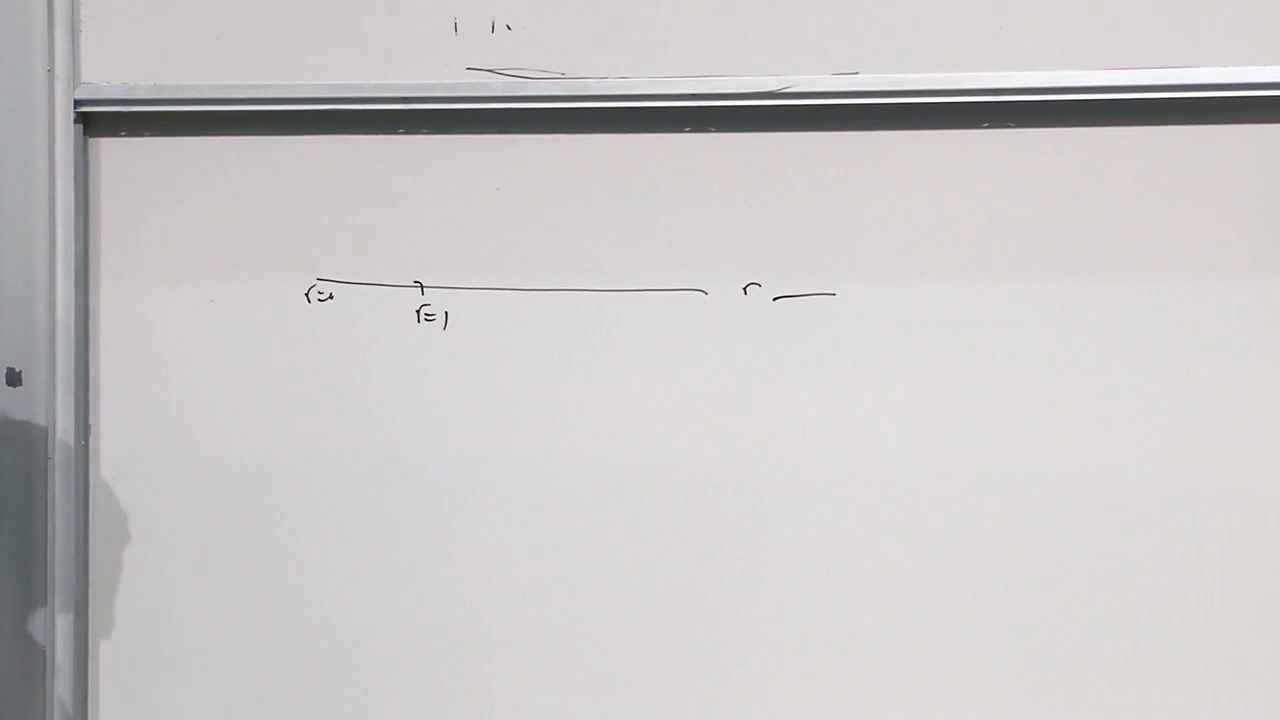
\includegraphics[width=0.78\textwidth]{lecture_07_figure_02.png}
\caption{La ligne de coordonnée radiale tracée au tableau. L’horizon se trouve en \(r=1\), tandis que \(r=0\) est la singularité de courbure.}
\lectureframe{00:16:11}
\end{figure}

Fixons \(t\) et les angles. L’élément de longueur spatiale positif est alors
\begin{equation}
ds^2=\frac{dr^2}{1-\frac1r},
\qquad
ds=\sqrt{\frac{r}{r-1}}\,dr.
\label{eq:l7-radial-proper-line}
\end{equation}
Définissons la distance propre sans dimension à l’horizon par
\begin{equation}
\rho(r)
=
\int_1^r\sqrt{\frac{r'}{r'-1}}\,dr'.
\label{eq:l7-rho-definition}
\end{equation}
Lorsque l’échelle globale est rétablie, la distance physique vaut \(r_{\mathrm S}\rho\). Nous n’aurons pas besoin de la forme explicite de l’intégrale. Seule sa dérivée nous importe :
\begin{equation}
\frac{d\rho}{dr}
=\sqrt{\frac{r}{r-1}},
\qquad
d\rho^2
=\frac{dr^2}{1-\frac1r}.
\label{eq:l7-rho-derivative}
\end{equation}
Le terme radial compliqué devient donc exactement \(-d\rho^2\). C’est pour cette simplification que nous introduisons \(\rho\).

Redimensionnons maintenant une nouvelle fois la coordonnée temporelle :
\begin{equation}
\omega=\frac{t}{2}.
\label{eq:l7-omega}
\end{equation}
Comme \(r\) est une fonction de \(\rho\), la métrique peut s’écrire
\begin{equation}
d\tau^2
=
F(\rho)\rho^2d\omega^2
-
d\rho^2
-
r(\rho)^2d\Omega_2^2.
\label{eq:l7-rho-metric}
\end{equation}

\begin{classroomqa}
\audiencequestion{La définition de \(F(\rho)\) vise-t-elle simplement à donner au coefficient temporel la forme \(F(\rho)\rho^2\) ?}
\lecturerresponse{Oui. À ce stade, cette factorisation n’a pas de contenu physique indépendant. C’est une définition commode. Son utilité apparaît lorsqu’on considère les limites de \(F\) près de l’horizon et loin de celui-ci.
\lecturetimestamp{00:26:39--00:26:59}}
\end{classroomqa}

Loin du trou noir, le coefficient temporel de Schwarzschild tend vers un. Comme \(dt=2d\omega\), on obtient
\begin{equation}
\lim_{\rho\to\infty}F(\rho)\rho^2=4.
\label{eq:l7-far-limit}
\end{equation}
Près de l’horizon, l’équation~\eqref{eq:l7-rho-definition} donne
\begin{equation}
\begin{aligned}
\rho&\simeq 2\sqrt{r-1},\\
r(\rho)&=1+\frac{\rho^2}{4}+O(\rho^4),\\
\lim_{\rho\to0}F(\rho)&=1.
\end{aligned}
\label{eq:l7-near-expansion}
\end{equation}

\begin{figure}[htbp]
\centering
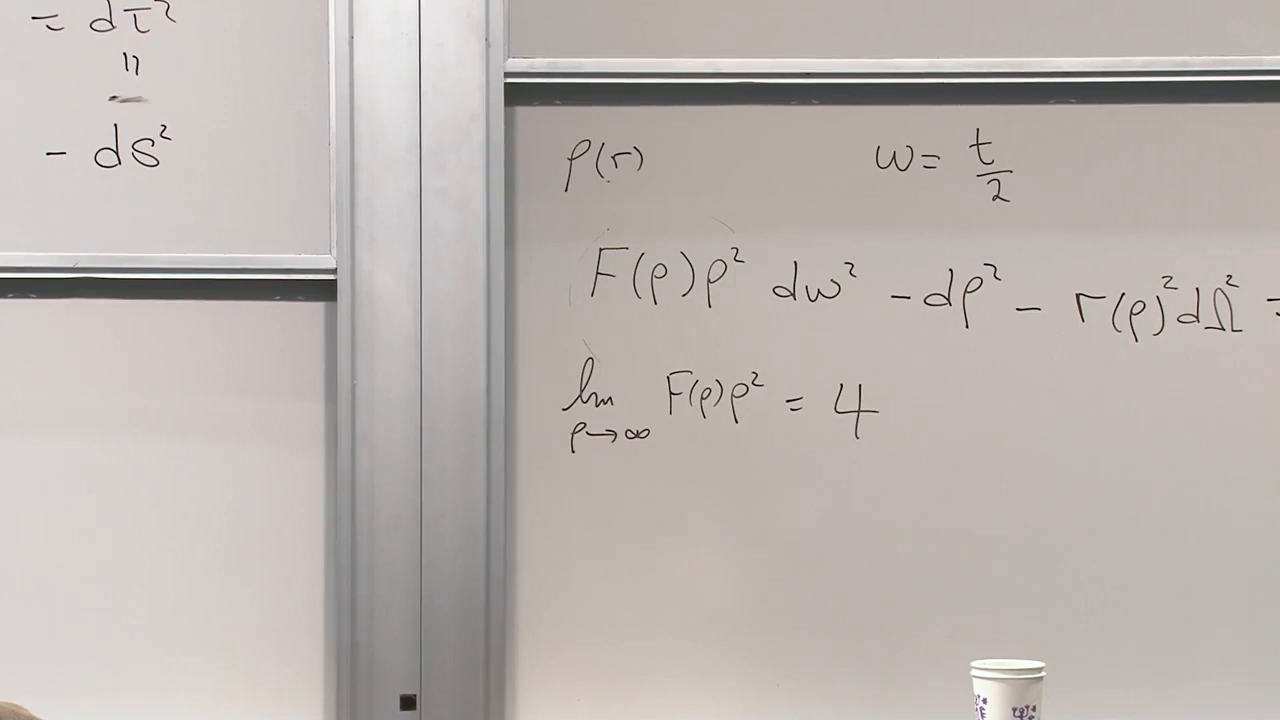
\includegraphics[width=0.90\textwidth]{lecture_07_figure_03.png}
\caption{La métrique en \((\rho,\omega)\), son coefficient temporel asymptotique et les limites près de l’horizon \(F\to1\) et \(r=1+\rho^2/4+\cdots\).}
\lectureframe{00:37:30}
\end{figure}

\section{L’espace-temps plat caché à l’horizon}

Au voisinage de \(\rho=0\), la partie radiale et temporelle de l’équation~\eqref{eq:l7-rho-metric} se réduit à
\begin{equation}
d\tau_{\mathrm{radial}}^2
\simeq
\rho^2d\omega^2-d\rho^2.
\label{eq:l7-rindler-metric}
\end{equation}
Il s’agit de l’espace-temps plat de Minkowski en coordonnées polaires hyperboliques. Définissons
\begin{equation}
X=\rho\cosh\omega,
\qquad
T=\rho\sinh\omega.
\label{eq:l7-rindler-transform}
\end{equation}
On obtient alors
\begin{equation}
dT^2-dX^2
=
\rho^2d\omega^2-d\rho^2.
\label{eq:l7-minkowski-check}
\end{equation}
Les courbes où \(\rho\) est constant vérifient
\begin{equation}
X^2-T^2=\rho^2
\label{eq:l7-constant-rho}
\end{equation}
ce sont des hyperboles. Les courbes où \(\omega\) est constant sont des demi-droites issues de l’origine. Lorsque \(\omega\to\infty\), ces demi-droites s’approchent de la droite nulle \(T=X\). L’horizon de Schwarzschild, qui semblait rejeté à un temps coordonné infini, est donc une droite nulle ordinaire dans le diagramme régulier.

\begin{figure}[htbp]
\centering
\includegraphics[width=0.88\textwidth]{lecture_07_figure_06.png}
\caption{La géométrie complète du tableau : hyperboles à \(\rho\) constant, demi-droites à \(\omega\) constant, horizon nul et région \(r<1\) au-dessus de celui-ci.}
\lectureframe{00:38:30}
\end{figure}

\begin{figure}[htbp]
\centering
\resizebox{0.96\linewidth}{!}{%
\begin{tikzpicture}[scale=1.02]
\draw[->] (-4.0,0) -- (4.1,0) node[right] {$X$};
\draw[->] (0,-0.3) -- (0,4.4) node[above] {$T$};
\draw[very thick] (0,0) -- (3.8,3.8)
  node[above right] {future horizon};
\draw[very thick] (0,0) -- (-3.8,3.8);
\draw[thick]
  plot[domain=0:1.42,samples=50]
  ({1.0*cosh(\x)},{1.0*sinh(\x)});
\draw[thick]
  plot[domain=0:1.05,samples=50]
  ({1.8*cosh(\x)},{1.8*sinh(\x)});
\draw[thick]
  plot[domain=0:1.42,samples=50]
  ({-1.0*cosh(\x)},{1.0*sinh(\x)});
\draw[thick]
  plot[domain=0:1.05,samples=50]
  ({-1.8*cosh(\x)},{1.8*sinh(\x)});
\draw[thin] (0,0) -- (3.8,1.55);
\draw[thin] (0,0) -- (3.8,2.65);
\draw[thin] (0,0) -- (-3.8,1.55);
\draw[thin] (0,0) -- (-3.8,2.65);
\draw[very thick,decorate,decoration={snake,amplitude=1.2pt,segment length=7pt}]
  (-2.6,4.0) .. controls (-1.2,3.5) and (1.2,3.5) .. (2.6,4.0);
\node at (0,4.18) {$r=0$};
\node at (2.2,0.7) {$\rho=\mathrm{constant}$};
\node at (2.55,2.25) {$\omega=\mathrm{constant}$};
\node at (0.9,3.28) {$r<1$};
\node at (2.8,3.35) {$r>1$};
\end{tikzpicture}
}
\caption{Une reconstruction causale nette. L’horizon est une droite nulle, tandis que la singularité de courbure \(r=0\) est une frontière future à l’intérieur du trou noir.}
\label{fig:l7-kruskal-clean}
\end{figure}

La limite où \(\rho\) devient petit diffère de la limite de petit rayon en coordonnées polaires euclidiennes. Un petit cercle euclidien se contracte vers un point. Une hyperbole à \(\rho\) constant s’approche d’une droite nulle entière. Ainsi, \(\rho=0\) désigne tout l’horizon, et pas seulement le point où les axes se croisent.

La formule extérieure peut être prolongée analytiquement jusqu’à \(r<1\). Près de l’horizon, \(r-1\simeq\rho^2/4\), de sorte que l’intérieur correspond formellement à \(\rho^2<0\). On peut qualifier \(\rho\) d’imaginaire, mais il est plus simple d’utiliser \(\rho^2\), \(r\) ou les coordonnées régulières \(T,X\). Les signes des coefficients de Schwarzschild associés à \(t\) et \(r\) s’échangent à l’intérieur. Cela ne signifie pas que la montre-bracelet physique se transforme en règle. Cela signifie que les coordonnées de Schwarzschild ont échangé leur caractère causal.

\begin{classroomqa}
\audiencequestion{Que représentent les hyperboles horizontales à l’intérieur de l’horizon, et que représentent les demi-droites ?}
\lecturerresponse{Les courbes hyperboliques correspondent à \(r\) constant, ou, de manière équivalente, à \(\rho^2\) constant, prolongé dans \(r<1\). Les demi-droites correspondent à un temps de Schwarzschild constant. À l’extérieur, elles forment un quadrillage commode pour les coordonnées ; à l’intérieur, il ne faut pas confondre ces mêmes étiquettes avec les trajectoires d’observateurs physiques.
\lecturetimestamp{00:44:12--00:44:59}}
\end{classroomqa}

\begin{classroomqa}
\audiencequestion{La direction verticale est-elle une coordonnée temporelle, et à quel référentiel correspond-elle ?}
\lecturerresponse{C’est une direction temporelle régulière dans le nouveau diagramme d’espace-temps, mais ce n’est pas le temps de Schwarzschild singulier \(t\). Le diagramme est adapté à la structure causale de la chute libre. Un observateur maintenu à rayon extérieur constant suit une hyperbole et doit accélérer ; un observateur en chute libre traverse l’horizon nul sans heurt.
\lecturetimestamp{00:45:54--00:46:48}}
\end{classroomqa}

\begin{classroomqa}
\audiencequestion{Si \(\rho^2<0\) à l’intérieur, où se trouve le facteur explicite \(i\) ?}
\lecturerresponse{On peut introduire un \(\rho\) imaginaire, mais cela n’apporte rien. Le contenu invariant est porté par \(r\), par \(\rho^2\) et par les coordonnées réelles et régulières \(T,X\). La relation \(r-1\simeq\rho^2/4\) n’est que le développement au voisinage de l’horizon.
\lecturetimestamp{00:52:35--00:53:00}}
\end{classroomqa}

Dans le cours, le diagramme régulier est souvent appelé diagramme de Kruskal. À proprement parler, les coordonnées exactes de Kruskal comprennent un facteur radial qui rend régulière la métrique de Schwarzschild complète, tandis que l’équation~\eqref{eq:l7-rindler-transform} en est la forme au voisinage de l’horizon. Le message causal reste le même : l’horizon est régulier, mais toute courbe future de genre temps ou nulle à l’intérieur se termine en \(r=0\). Aucun virage supraluminique ne peut la ramener à travers l’horizon.

\subsection{Comment la singularité de coordonnées a été comprise}

La régularité de l’horizon a longtemps été difficile à discerner, car les coordonnées originales de Schwarzschild donnent à ses coefficients une apparence singulière. Eddington, puis Finkelstein, ont introduit des coordonnées qui traversent l’horizon, et Finkelstein a reconnu la frontière causale à sens unique. Kruskal, qui maîtrisait les changements de coordonnées grâce à la physique des plasmas, a fourni une représentation globale régulière de la solution éternelle.

Le cours s’interrompt ensuite pour évoquer John Wheeler, qui a contribué à imposer l’expression « trou noir ». Cette pause est aussi personnelle qu’historique : Wheeler est resté dans les mémoires comme un ami doux et réfléchi, même si les jugements politiques, notamment sur la compétition nucléaire, divergeaient fortement. Une anecdote personnelle humoristique est racontée pour éviter de réduire Wheeler à une figure socialement conventionnelle. Le propos technique reprend avec la réplique : « les trous noirs n’ont pas de cheveux ». Un trou non rotatif perturbé retrouve rapidement une symétrie sphérique ; un trou en rotation évolue vers la forme stationnaire déterminée par ses paramètres conservés. C’est la version qualitative, dans ce cours, de l’idée d’absence de cheveux, et non une démonstration du théorème complet.

\section{Alice traverse l’horizon ; Bob reste à l’extérieur}

Le diagramme maximalement prolongé contient des régions qui n’existent pas dans l’espace-temps simple d’une étoile s’effondrant à partir de données initiales ordinaires. Pour l’expérience avec les observateurs, nous n’utilisons que l’extérieur, l’horizon futur et l’intérieur du trou noir.

\begin{figure}[htbp]
\centering
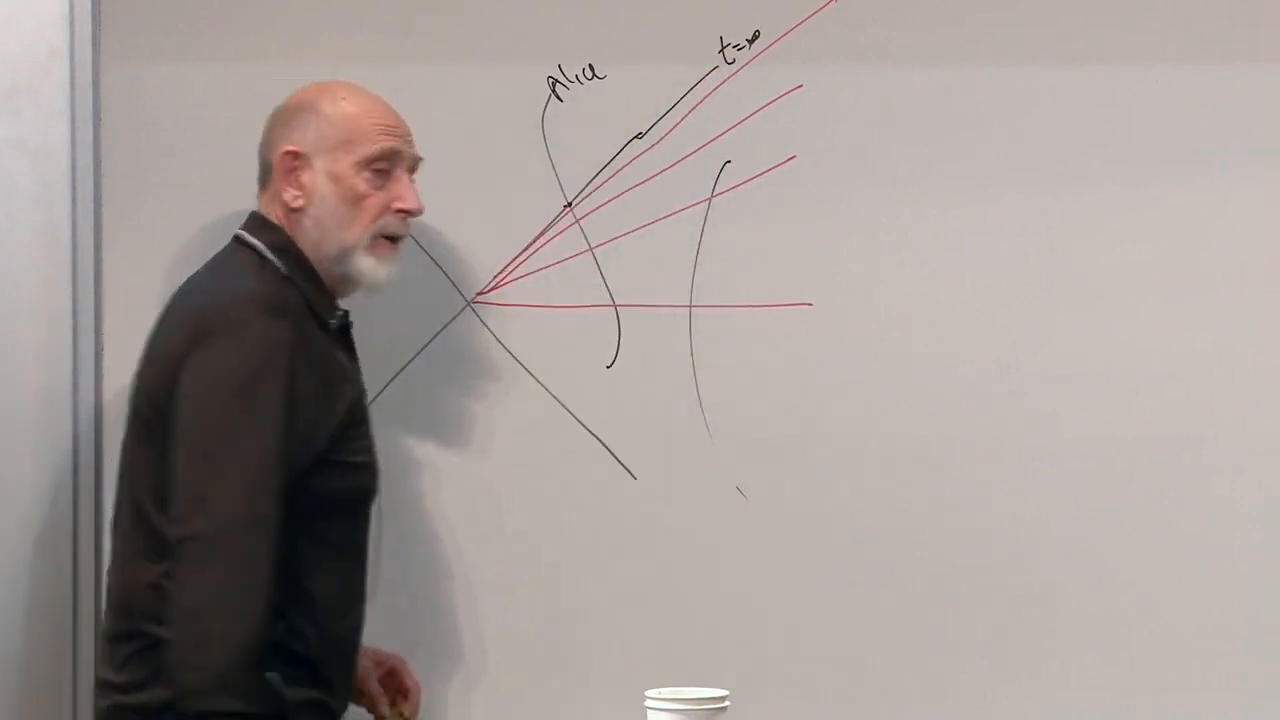
\includegraphics[width=0.84\textwidth]{lecture_07_figure_04.png}
\caption{La ligne d’univers d’Alice en chute et les demi-droites de temps de Schwarzschild constant. La demi-droite limite porte l’étiquette \(t=\infty\).}
\lectureframe{00:54:54}
\end{figure}

Alice est en chute libre. Sa ligne d’univers traverse l’horizon et atteint la singularité en un temps propre fini. Si le trou noir est assez grand pour que les forces de marée y soient faibles, rien de singulier n’arrive à son horloge à l’horizon.

Bob, lui, reste à rayon extérieur constant. Pour maintenir cette position, il doit accélérer. Les signaux lumineux émis à des instants de plus en plus tardifs sur la trajectoire d’Alice lui parviennent avec un retard croissant et un décalage vers le rouge de plus en plus prononcé. En temps de Schwarzschild, Alice s’approche de \(t=\infty\), et Bob ne reçoit jamais de signal émis après la traversée de son horizon. Ce sont des affirmations sur les signaux causaux et sur le feuilletage extérieur, et non des indices de l’existence d’une surface matérielle à l’horizon.

\begin{classroomqa}
\audiencequestion{Si Bob voit Alice ralentir, Alice doit-elle voir Bob accélérer ?}
\lecturerresponse{Non. Alice continue de recevoir des signaux lumineux ordinaires de Bob tant que sa ligne d’univers dure. Il existe un dernier événement sur la ligne d’univers de Bob qui peut lui parvenir, mais cet événement n’est le dernier que parce qu’Alice atteint ensuite la singularité. Rien n’arrive brusquement à Bob. Toute observation porte sur un cône de lumière passé, et les deux lignes d’univers entretiennent une relation causale asymétrique.
\lecturetimestamp{00:58:31--01:01:23}}
\end{classroomqa}

\begin{classroomqa}
\audiencequestion{Si Bob sait que, dans ses coordonnées, Alice est encore près de l’horizon, peut-il descendre, la récupérer et revenir ?}
\lecturerresponse{Une ligne d’univers de sauvetage doit rejoindre Alice avant qu’elle traverse l’horizon des événements. Après cet événement, aucun trajet futur ne peut la rejoindre puis revenir à l’extérieur. Le fait que les tranches de Schwarzschild situent la traversée en \(t=\infty\) ne signifie pas qu’Alice reste assise sur une surface matérielle où l’on pourrait la récupérer ; cela montre que ces tranches ne fournissent pas de notion globale de « maintenant » à travers l’horizon.
\lecturetimestamp{01:01:24--01:02:12}}
\end{classroomqa}

\section{Charlie suit Alice}

Faisons tomber Charlie à peu de distance derrière Alice. Tous deux sont alors approximativement inertiels près de l’horizon. Ils peuvent échanger des signaux, converser dans les deux sens ou même se tenir la main. Aucun des deux ne voit de panneau indiquant l’horizon. La différence avec Bob ne tient pas à l’identité des trois personnes, mais à celle entre la chute libre et une ligne d’univers accélérée qui reste à l’extérieur.

\begin{classroomqa}
\audiencequestion{Que voit Bob si Alice tombe la première et que Charlie la suit, comme un ballon de basket qui suit un anneau ?}
\lecturerresponse{Bob voit tous deux s’approcher de l’horizon. Alice, qui est devant, lui paraît ralentir progressivement et se comprimer radialement la première. Charlie semble se rapprocher de plus en plus d’elle, mais ne la rattrape jamais dans la vue limite de Bob depuis l’extérieur. Cette accumulation apparente ne décrit pas ce que ressent l’un ou l’autre des deux objets en chute.
\lecturetimestamp{01:04:12--01:06:05}}
\end{classroomqa}

\begin{classroomqa}
\audiencequestion{L’aplatissement apparent contredit-il la force de marée, qui devrait étirer l’objet en chute dans la direction radiale ?}
\lecturerresponse{Ce sont des effets différents. L’aplatissement relève de la description de Bob en coordonnées de Schwarzschild. L’allongement de marée est un effet local de la courbure que ressentent Alice et Charlie. La discussion suppose que le trou noir est assez grand, ou les observateurs assez petits, pour que l’effet de marée à l’horizon soit négligeable. Un trou noir d’environ une masse solaire produirait au contraire de fortes marées à l’horizon, tandis qu’elles peuvent être faibles pour un trou noir supermassif.
\lecturetimestamp{01:06:07--01:08:18}}
\end{classroomqa}

\begin{classroomqa}
\audiencequestion{Charlie voit-il Alice traverser l’horizon alors qu’il est encore à l’extérieur ?}
\lecturerresponse{Traçons le rayon nul. La lumière émise lors de la traversée d’Alice suit l’horizon et atteint Charlie au moment où celui-ci le traverse. À cet événement, il peut calculer qu’il a vu Alice traverser, même si aucun des deux observateurs ne rencontre de marqueur local. Ensuite, il peut la voir à l’intérieur. S’il accélère pour s’éloigner avant la traversée et parvient à rester à l’extérieur, il ne voit jamais la traversée.
\lecturetimestamp{01:08:19--01:11:11}}
\end{classroomqa}

\begin{classroomqa}
\audiencequestion{Si Alice est déjà à l’intérieur tandis que Charlie est à l’extérieur, comment comparer leurs rayons ultérieurs et leurs instants de traversée ?}
\lecturerresponse{Il n’existe pas de relation de simultanéité indépendante de l’observateur que l’on puisse déduire d’une expression comme « au même instant ». Alice voit Charlie sur son cône de lumière passé et ne peut voir sa traversée ultérieure que lorsqu’elle se trouve plus loin à l’intérieur. Ce sont les lignes d’univers et les rayons nuls précis qui répondent à la question. Pour généraliser à de nombreux objets en chute largement séparés, il faut tracer leur diagramme causal réel, au lieu de supposer un instant de traversée universel.
\lecturetimestamp{01:11:14--01:12:31}}
\end{classroomqa}

Dans les coordonnées régulières du voisinage de l’horizon, une trajectoire de chute libre est presque une droite. Elle n’est pas exactement rectiligne dans la géométrie complète de Schwarzschild, mais cette approximation devient bonne près d’un horizon vaste et faiblement courbé.

\begin{classroomqa}
\audiencequestion{La théorie des cordes peut-elle déterminer ce qui se passe dans le régime de gravité quantique à l’intérieur du trou noir ?}
\lecturerresponse{C’est précisément là que le sujet devient subtil. Une théorie quantique de la gravité est nécessaire près de la singularité, et la théorie des cordes est une candidate possible, mais les questions pertinentes étaient encore ouvertes et difficiles ; une simple application du diagramme classique ne les avait pas résolues.
\lecturetimestamp{01:13:04--01:13:38}}
\end{classroomqa}

\begin{classroomqa}
\audiencequestion{Que deviennent l’horloge et la vitesse propres d’Alice lorsqu’elle traverse l’horizon ?}
\lecturerresponse{Son horloge continue de battre à son rythme local ordinaire et mesure un temps propre fini. Dans son référentiel instantané de repos, elle est au repos ; relativement à un référentiel local en chute libre, sa vitesse est finie et ordinaire. Près d’un horizon vaste, la géométrie est presque plate, si bien que les marques régulièrement espacées en temps propre sur sa ligne d’univers restent régulières jusqu’à ce que la courbure devienne forte près de la singularité.
\lecturetimestamp{01:13:39--01:14:44}}
\end{classroomqa}

\begin{classroomqa}
\audiencequestion{Que se passe-t-il si Bob accélère vers l’extérieur, mais pas assez pour éviter de tomber à travers l’horizon ?}
\lecturerresponse{Sa ligne d’univers se courbe alors vers l’extérieur, mais traverse tout de même l’horizon. S’il le traverse très tard, il peut voir Alice peu après sa propre traversée, mais le temps propre qui lui reste avant la singularité est court. Les pentes des lignes d’univers sur le croquis ne sont pas des étalons ni des horloges gradués ; c’est l’ordre causal, et non leurs longueurs euclidiennes dessinées, qui est préservé.
\lecturetimestamp{01:14:47--01:16:31}}
\end{classroomqa}

Toutes ces conclusions supposent qu’aucun signal ne dépasse la vitesse de la lumière. Le cours plaisante brièvement au sujet de reportages de presse récents à l’époque, qui évoquaient des neutrinos apparemment supraluminiques en Italie ; il s’agissait d’une allusion à une erreur de chronométrage expérimental, et non d’une exception à la relativité. La construction causale elle-même reste bornée par les droites nulles.

\begin{classroomqa}
\audiencequestion{Des horloges synchronisées portées par Alice et Bob peuvent-elles trancher la question si Alice plonge vers l’horizon puis revient ?}
\lecturerresponse{Ils peuvent comparer leurs horloges lorsqu’ils se retrouvent au même endroit, mais après la séparation de leurs lignes d’univers, il n’existe pas de synchronisation distante unique, surtout lorsque l’un d’eux change de mouvement. Traçons les deux lignes d’univers et les rayons nuls échangés. Ce diagramme donne la réponse opérationnelle à toute expérience spécifiée.
\lecturetimestamp{01:17:34--01:18:25}}
\end{classroomqa}

\begin{figure}[htbp]
\centering
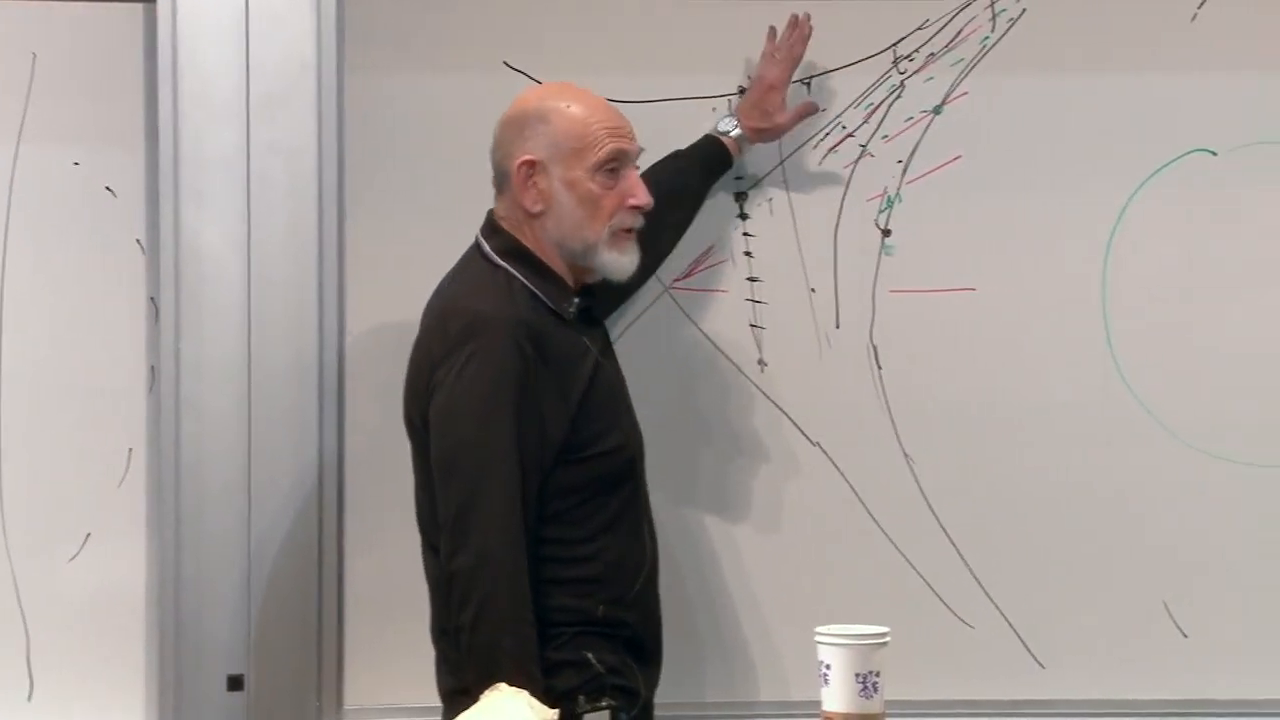
\includegraphics[width=0.86\textwidth]{lecture_07_figure_05.png}
\caption{Le diagramme causal construit progressivement pour répondre aux questions sur Alice, Bob et Charlie. Chaque observation se situe en traçant un rayon nul depuis l’événement observé jusqu’à la ligne d’univers de l’observateur.}
\lectureframe{01:18:12}
\end{figure}

\begin{figure}[htbp]
\centering
\resizebox{0.96\linewidth}{!}{%
\begin{tikzpicture}[scale=0.96]
\draw[very thick] (-3.8,-0.3) -- (3.8,4.5);
\node[above right] at (3.8,4.5) {future horizon};
\draw[very thick,decorate,decoration={snake,amplitude=1.2pt,segment length=7pt}]
  (-1.8,4.25) .. controls (0.1,3.72) and (2.0,3.92) .. (3.4,4.55);
\node at (0.3,4.48) {singularity};
\draw[thick,->]
  plot[smooth] coordinates {(-1.5,0.0) (-0.9,1.0) (-0.25,1.9)
  (0.55,2.75) (1.3,3.45) (2.1,4.0)};
\node[left] at (-0.4,2.0) {Alice};
\draw[thick,->]
  plot[smooth] coordinates {(-2.0,0.0) (-1.35,0.95) (-0.65,1.85)
  (0.15,2.7) (0.95,3.38) (1.75,3.92)};
\node[left] at (-1.15,1.55) {Charlie};
\draw[thick,->]
  plot[smooth] coordinates {(3.35,0.1) (3.0,0.9) (2.9,1.8)
  (2.98,2.8) (3.15,3.7)};
\node[right] at (3.05,2.0) {Bob};
\draw[thin,->] (-0.8,1.15) -- (2.94,2.0);
\draw[thin,->] (-0.15,2.0) -- (3.02,2.72);
\draw[thin,->] (3.0,1.2) -- (0.15,2.7);
\draw[fill] (0.55,2.75) circle (1.3pt);
\draw[fill] (0.15,2.7) circle (1.3pt);
\end{tikzpicture}
}
\caption{Schéma des observateurs. Les observations de Bob depuis l’extérieur et les observations mutuelles d’Alice et Charlie reposent sur des constructions distinctes de rayons nuls, et non sur des slogans de réciprocité entre horloges.}
\label{fig:l7-observers-clean}
\end{figure}

\begin{classroomqa}
\audiencequestion{Bob voit-il Alice pendant un temps infini, et cela signifie-t-il qu’elle ne meurt jamais dans sa réalité ?}
\lecturerresponse{Bob reçoit ses signaux pendant un intervalle de son temps qui n’est pas borné, mais il voit son horloge ralentir jusqu’à un rythme nul et ne reçoit que la suite finie de battements de cœur émis avant sa traversée. Le mot « réalité » masque la distinction entre un événement local et le relevé asymptotique d’un observateur. Alice ne voit pas son horloge s’arrêter à l’horizon ; les signaux reçus par Bob sont de plus en plus retardés et décalés vers le rouge.
\lecturetimestamp{01:18:32--01:20:59}}
\end{classroomqa}

\begin{classroomqa}
\audiencequestion{Une fois qu’Alice a traversé l’horizon, voit-elle soudain toute la matière ancienne qui paraissait figée à celui-ci ?}
\lecturerresponse{Rien ne se dégage brusquement. Pendant sa chute, les cônes de lumière passés qui lui permettent de voir la matière antérieure changent continûment. Elle peut déduire que la lumière qui lui parvient maintenant a été émise plus tôt et que la matière a traversé l’horizon avant elle. Le point de vue de Charlie sur Alice enseigne la même chose : aucune des traversées ne produit de discontinuité locale ni ne révèle un amas caché de chaises et de dinosaures.
\lecturetimestamp{01:21:02--01:23:48}}
\end{classroomqa}

\begin{classroomqa}
\audiencequestion{Existe-t-il des simulations réalistes de ce qu’un objet en chute verrait ?}
\lecturerresponse{Le cours renvoie aux visualisations de trous noirs d’Andrew Hamilton. Elles peuvent rendre perceptibles l’aberration marquée et les décalages de fréquence de la lumière entrante, même si l’image peut déconcerter davantage qu’éclairer. L’expression « rien de particulier à l’horizon » concerne la géométrie locale, et non l’apparence ordinaire du ciel.
\lecturetimestamp{01:24:11--01:25:29}}
\end{classroomqa}

\section{D’un trou éternel à un trou en croissance}

Le sommet inférieur du diagramme éternel maximalement prolongé a peu de signification directe pour un trou noir formé par l’effondrement d’une étoile. Dans la géométrie simple de l’effondrement, seule apparaît la partie contenant l’extérieur, l’horizon futur et l’intérieur futur. Cette distinction devient essentielle lorsque la matière peut faire varier la masse du trou noir.

\begin{classroomqa}
\audiencequestion{Quel événement physique représente le sommet inférieur du diagramme idéalisé ?}
\lecturerresponse{Dans la solution mathématique éternelle, il fait partie du prolongement maximal. Un trou noir formé par l’effondrement de matière ne contient pas toute cette région inférieure. Son horizon a une histoire de formation, qui exige un autre diagramme global et sera étudiée au cours suivant.
\lecturetimestamp{01:25:59--01:26:52}}
\end{classroomqa}

Lorsqu’un petit corps d’épreuve tombe dans le trou noir, on peut négliger sa rétroaction et le diagramme de Schwarzschild fixe suffit. Si une masse importante tombe dans le trou noir, la masse de celui-ci et le rayon de Schwarzschild augmentent :
\begin{equation}
r_{\mathrm S}=2GM,
\qquad
\Delta r_{\mathrm S}=2G\,\Delta M.
\label{eq:l7-growing-radius}
\end{equation}
L’horizon se déforme vers l’objet entrant, les horizons se rejoignent et l’horizon commun déformé se stabilise rapidement. Dans l’idéalisation non rotative du cours, l’état final est une sphère légèrement plus grande. Une fusion réelle rayonne aussi de l’énergie sous forme d’ondes gravitationnelles et laisse généralement un trou noir en rotation.

\begin{classroomqa}
\audiencequestion{Si l’horizon grandit lorsqu’une masse tombe dans le trou noir, se déplace-t-il vers l’extérieur pour rejoindre la matière qui semblait figée près de l’ancien horizon ?}
\lecturerresponse{Pour un objet entrant suffisamment massif, l’approximation de la particule d’épreuve n’est plus valable. L’horizon se déforme, rejoint la région piégée de l’objet entrant et se détend vers un horizon stationnaire plus grand. La position exacte de l’horizon des événements est de nature globale et peut s’étendre dans une région antérieure à l’arrivée de la matière. Le cours reporte délibérément la construction complète à la prochaine séance.
\lecturetimestamp{01:26:55--01:29:05}}
\end{classroomqa}

\begin{classroomqa}
\audiencequestion{Pourquoi les astronomes peuvent-ils observer des éclats lumineux si la matière met un temps de Schwarzschild infini à atteindre l’horizon ?}
\lecturerresponse{Le rayonnement lumineux intense ne provient pas de l’horizon lui-même. Dans un flux ou un disque d’accrétion, le gaz entre en collision et s’échauffe à l’extérieur de l’horizon, notamment près des orbites photoniques fortement courbées. Ce plasma extérieur peut émettre de la lumière qui nous parvient. La géométrie vide de Schwarzschild isole le problème causal, mais ne constitue pas un modèle complet d’un environnement astrophysique.
\lecturetimestamp{01:29:07--01:30:22}}
\end{classroomqa}

Le temps caractéristique de relaxation est fixé par le temps de traversée de la lumière :
\begin{equation}
t_{\mathrm{cross}}\sim\frac{r_{\mathrm S}}{c},
\qquad
t_{\mathrm{relax}}\sim
\text{a few to a few tens of }t_{\mathrm{cross}}.
\label{eq:l7-relaxation-scale}
\end{equation}
Le cours estime que \(10^{-5}\,\mathrm{s}\) correspond au temps de traversée d’un trou noir de l’ordre du kilomètre et qu’il faut environ \(10^{-3}\,\mathrm{s}\) pour qu’une petite fusion devienne presque stationnaire. Pour un trou noir d’un milliard de masses solaires, le temps correspondant se compte en minutes ou en heures. Ce sont des estimations d’échelle, et non des calculs précis de fusion. C’est la succession géométrique qui importe : haltère, cacahuète, presque sphérique, stationnaire.

\begin{classroomqa}
\audiencequestion{À quelle vitesse un horizon déformé ou issu d’une fusion récente se stabilise-t-il ?}
\lecturerresponse{Sur une échelle de temps qui ne dépasse pas de beaucoup le temps nécessaire à la lumière pour traverser le trou noir. Comme toutes les longueurs et tous les temps varient avec \(r_{\mathrm S}\), les petits trous noirs se stabilisent en une fraction de seconde, tandis que les trous supermassifs le font selon des temps d’horloge beaucoup plus longs. L’absence de cheveux décrit l’état final stationnaire ; la déformation transitoire évacue de l’énergie sous forme de rayonnement gravitationnel.
\lecturetimestamp{01:30:26--01:33:18}}
\end{classroomqa}

\begin{classroomqa}
\audiencequestion{Que voit Bob si de la matière tombée plus tôt se trouve entre l’ancien et le nouvel horizon tandis qu’un autre corps massif tombe dans le trou noir ?}
\lecturerresponse{Il est impossible de répondre de manière cohérente à cette question en raccordant deux diagrammes statiques de Schwarzschild. Il faut résoudre ou construire la géométrie d’effondrement dépendante du temps et déterminer la position de son horizon global. Le cours laisse la question en suspens et reporte explicitement la réponse à la semaine suivante, consacrée à la formation des horizons.
\lecturetimestamp{01:33:20--01:35:41}}
\end{classroomqa}

\section{Que change la variation d’échelle ?}

Le diagramme sans dimension ne change pas lorsque \(r_{\mathrm S}\) varie. En revanche, la signification physique d’un intervalle dessiné change :
\begin{equation}
d\tau_{\mathrm{physical}}^2
=
r_{\mathrm S}^2\,d\hat{\tau}^2,
\qquad
\ell_{\mathrm{physical}}
=
r_{\mathrm S}\,\hat{\ell}.
\label{eq:l7-scale-restoration}
\end{equation}
Une séparation sans dimension qui représente un demi-kilomètre pour un trou noir de l’ordre du kilomètre en représente environ un demi-milliard de kilomètres pour un trou noir mille millions de fois plus grand. L’analogie des sphères dessinées à la même taille revient ici : la forme reste la même, tandis que le nombre de mètres étalons représenté par une ligne varie avec le rayon.

\begin{classroomqa}
\audiencequestion{Comment le diagramme causal change-t-il lorsque le rayon de Schwarzschild varie ?}
\lecturerresponse{Il ne change pas une fois le rayon éliminé par changement d’échelle. Chaque longueur et chaque durée physique attribuée au diagramme est multipliée par \(r_{\mathrm S}\), tandis que la courbure aux points sans dimension correspondants est multipliée par \(r_{\mathrm S}^{-2}\).
\lecturetimestamp{01:35:41--01:38:10}}
\end{classroomqa}

\begin{classroomqa}
\audiencequestion{La conclusion causale change-t-elle si Bob est en orbite plutôt que de rester à une position angulaire fixe ?}
\lecturerresponse{Les décalages vers le rouge détaillés et les directions d’arrivée deviennent plus complexes, mais la séparation causale due à l’horizon ne change pas. Aucune orbite temporelle extérieure ne reçoit de signal émis depuis l’intérieur de l’horizon.
\lecturetimestamp{01:38:12--01:38:26}}
\end{classroomqa}

\begin{classroomqa}
\audiencequestion{Puisque la gravité s’annule à l’intérieur d’une coquille sphérique, s’annule-t-elle aussi à l’intérieur de l’horizon parce que la masse du trou noir est répartie sur cette surface ?}
\lecturerresponse{Non. L’horizon des événements n’est pas une coquille matérielle qui porterait la masse. Le théorème newtonien des coquilles ne s’y applique donc pas. Le cours compare la solution statique extérieure à une source ponctuelle située à la singularité de courbure, mais la matière qui tombe actuellement au cours de la formation du trou noir exige la géométrie dépendant du temps, qui sera étudiée au cours suivant.
\lecturetimestamp{01:38:28--01:40:41}}
\end{classroomqa}

\section{Rotation et géométrie radiale}

Le moment cinétique subsiste après l’effondrement. La géométrie extérieure d’un trou noir en rotation diffère de celle de Schwarzschild : sa solution stationnaire est celle de Kerr, la rotation déforme la géométrie de l’horizon et l’entraînement des référentiels fait tourner les directions inertielles autour du trou. En principe, on mesure le moment cinétique à partir de ces effets gravitationnels extérieurs. La matière ne perd pas son moment cinétique simplement en franchissant un horizon.

\begin{classroomqa}
\audiencequestion{Un trou noir peut-il avoir un moment cinétique mesurable, et la rotation modifie-t-elle la gravité à l’extérieur ?}
\lecturerresponse{Oui. Le moment cinétique subsiste comme paramètre conservé, déforme la géométrie stationnaire et produit un entraînement des référentiels. L’horizon n’est plus le simple horizon sphérique de Schwarzschild. Le cours compare qualitativement cette déformation à la forme aplatie de la Terre, tout en soulignant que la solution complète en rotation est nettement plus complexe.
\lecturetimestamp{01:40:45--01:42:36}}
\end{classroomqa}

\begin{classroomqa}
\audiencequestion{La relation entre \(r\) et la distance propre \(\rho\) signifie-t-elle que la gravité contracte l’espace ?}
\lecturerresponse{La distance radiale propre \(\rho\) vérifie
\begin{equation*}
\frac{d\rho}{dr}=\sqrt{\frac{r}{r-1}}>1
\end{equation*}
À l’extérieur de l’horizon unité. Un accroissement coordonné donné \(dr\) correspond donc à un intervalle radial propre plus grand près de l’horizon. Dire que l’espace est contracté ou étiré dépend des intervalles de coordonnées que l’on compare. L’énoncé invariant est la relation entre les distances propres elle-même.
\lecturetimestamp{01:42:36--01:43:20}}
\end{classroomqa}

\section{Questions finales}

\begin{classroomqa}
\audiencequestion{Du point de vue de Bob, l’horloge d’Alice semble s’arrêter. Du point de vue d’Alice, l’espace ou le temps de Bob prend-il fin ?}
\lecturerresponse{Non. Alice voit les signaux ordinaires provenant d’événements successifs sur la ligne d’univers de Bob, jusqu’à ce que sa propre ligne d’univers prenne fin. Elle ne voit pas les événements ultérieurs de Bob parce qu’aucun point ultérieur n’existe sur sa ligne d’univers, et non parce que Bob ou son espace disparaît. Dans ces coordonnées causales régulières, les rayons lumineux radiaux sont représentés par des lignes droites ; leur apparence de trajectoires courbes dans un autre système de coordonnées ne change pas les événements qu’ils relient.
\lecturetimestamp{01:43:21--01:45:20}}
\end{classroomqa}

La relativité générale comporte deux tâches complémentaires. Étant donnée une métrique, on peut tracer les géodésiques et les rayons lumineux afin de déterminer ce que mesurent les observateurs. Étant donnée une distribution de matière, il faut résoudre les équations d’Einstein pour trouver la métrique. La première tâche a occupé ce cours. La seconde est généralement plus difficile, bien que l’effondrement avec symétrie fournisse des exemples traitables.

\begin{classroomqa}
\audiencequestion{Qu’advient-il de l’horizon et de la singularité d’un trou noir qui s’évapore ?}
\lecturerresponse{Le cours présente un schéma qualitatif dans lequel l’horizon se rétrécit et rejoint l’extrémité de la région singulière. L’évaporation est un processus quantique semi-classique, et le devenir final à l’échelle de Planck n’est pas déterminé par le diagramme classique de Schwarzschild. Il faut donc voir ce schéma de rétrécissement comme un aperçu qualitatif, et non comme une géométrie quantique complète.
\lecturetimestamp{01:46:04--01:46:32}}
\end{classroomqa}

Presque tous les trous noirs astrophysiques devraient être en rotation. Les étoiles possèdent déjà un moment cinétique, et l’effondrement amplifie leur vitesse angulaire à la manière bien connue d’un patineur qui ramène les bras vers lui. La structure singulière d’un trou noir de Kerr n’est pas la surface de Schwarzschild \(r=0\) représentée ici ; il ne faut pas la décrire comme de la matière tournant littéralement à une vitesse linéaire infinie.

\begin{classroomqa}
\audiencequestion{Les trous noirs macroscopiques sans rotation sont-ils courants, et combien y a-t-il de trous noirs ?}
\lecturerresponse{Un moment cinétique exactement nul serait une idéalisation exceptionnelle. Le cours ne donne qu’une estimation pédagogique très approximative de la population cosmique, comprise entre les nombres de galaxies et d’étoiles, et peut-être de l’ordre de \(10^{15}\). Il s’agit d’une estimation datant du cours, et non d’un recensement mesuré. Le point solide est que l’effondrement conserve et amplifie généralement une partie du moment cinétique.
\lecturetimestamp{01:46:32--01:48:42}}
\end{classroomqa}

\begin{classroomqa}
\audiencequestion{Les trous noirs se forment-ils à partir de matière préexistante ou apparaissent-ils par un processus quantique ?}
\lecturerresponse{Les trous noirs astrophysiques ordinaires se forment lorsque de la matière stellaire existante s’effondre. La combustion nucléaire et le flux d’énergie vers l’extérieur contribuent à soutenir une étoile. Lorsque son combustible est épuisé, le résidu se contracte. Selon sa masse et les mécanismes de soutien par la pression dont il dispose, il peut devenir une naine blanche ou une étoile à neutrons ; si aucun soutien ne peut arrêter l’effondrement, il peut aussi passer sous son propre rayon de Schwarzschild et former un trou noir.
\lecturetimestamp{01:48:43--01:50:23}}
\end{classroomqa}

\begin{classroomqa}
\audiencequestion{Des trous noirs microscopiques pourraient-ils se former, et qu’est-ce qui déterminerait leur durée de vie et leur taille minimale ?}
\lecturerresponse{Cette partie est spéculative. L’évaporation de Hawking est d’autant plus rapide que la masse est faible, et la durée de vie varie approximativement comme \(M^3\). Le cours compare un trou noir dont la durée de vie pourrait être cosmologique à une montagne en termes de masse ; cette analogie numérique n’est qu’approximative. Des fluctuations très fortes de densité dans l’Univers primordial ou des collisions suffisamment énergétiques pourraient constituer des mécanismes de formation. Un trou noir proche de la masse de Planck, soit environ \(10^{-5}\,\mathrm{g}\), marque l’échelle à laquelle une description géométrique classique cesse d’être fiable. Selon une extrapolation directe, atteindre cette énergie dans un accélérateur ordinaire exigerait une machine d’une taille invraisemblable, même si la formation est possible en principe.
\lecturetimestamp{01:50:23--01:53:31}}
\end{classroomqa}

\begin{classroomqa}
\audiencequestion{Le cours abordera-t-il la cosmologie, la matière noire, l’énergie noire, l’entropie et les ondes gravitationnelles ?}
\lecturerresponse{Les applications cosmologiques et, peut-être, les ondes gravitationnelles restent des sujets possibles pour la suite. L’entropie des trous noirs est reportée au-delà du trimestre. Le cours se conclut en reconnaissant que seulement environ un quart du programme prévu a été couvert ce soir-là : répondre soigneusement aux questions compte davantage que de parcourir le plan à toute vitesse.
\lecturetimestamp{01:53:33--01:54:38}}
\end{classroomqa}

La règle opérationnelle résiste à toutes les questions posées dans la salle. Précisez les lignes d’univers, tracez les rayons lumineux et repérez les événements qu’ils relient. L’horizon n’est pas un lieu où la physique locale cesse de fonctionner ; c’est la frontière au-delà de laquelle tout signal dirigé vers le futur reste à l’intérieur. Le cours suivant remplacera le fond éternel par une source en effondrement et montrera comment cette frontière se forme.
\graphicspath{{../../../generated_course_notes/core/general_relativity/2012_fall_theoretical_minimum/chapters/lecture_08/}{../../../generated_course_notes/core/general_relativity/2012_fall_theoretical_minimum/figures/}{../../../generated_course_notes/core/general_relativity/2012_fall_theoretical_minimum/assets/}}
\chapter{Diagrammes de Penrose et formation d’un véritable trou noir}

Le diagramme de Kruskal décrit avec élégance le voisinage d’un horizon de Schwarzschild, mais un véritable trou noir n’est pas éternel : il se forme lors de l’effondrement de matière. Quelles parties du diagramme étendu subsistent après cette évolution physique ? Pour répondre, il nous faut un diagramme assez vaste pour contenir un espace-temps entier et assez rigoureux pour préserver le mouvement de la lumière. Nous commencerons par compactifier l’espace-temps plat, puis l’espace-temps de Schwarzschild, et enfin nous raccorderons les parties appropriées de part et d’autre d’une couche de rayonnement qui s’effondre.

\section{Au voisinage de l’horizon : rappel sur Kruskal et ses quatre quadrants}

Nous reprenons exactement là où le cours précédent s’est arrêté. Tout près de l’horizon de Schwarzschild, la géométrie ressemble localement à celle d’un espace plat. L’horizon lui-même se comporte comme le lieu d’une coordonnée polaire hyperbolique, un peu comme dans les coordonnées accélérées de l’espace-temps ordinaire de Minkowski. Dans cette représentation locale, nous imposons dès le départ une règle à laquelle nous ne dérogerons jamais : les rayons lumineux radiaux sont tracés à \(45^\circ\), et toute ligne d’univers de genre temps doit rester plus pentue que ces lignes de genre lumière.

Il vaut mieux considérer les coordonnées de ce rappel comme le temps et l’espace tels que les perçoit un observateur en chute libre. Dans ces coordonnées localement inertielles, le voisinage de l’horizon paraît presque plat. Mais un observateur qui tient à rester en suspension à rayon constant à l’extérieur du trou noir n’est pas inertiel. Dans le référentiel en chute libre, sa ligne d’univers est accélérée. Plus on se maintient près de l’horizon, plus l’accélération nécessaire pour y rester est grande. C’est ce que représentent physiquement les courbes extérieures dessinées sur la partie droite du tableau.

\begin{figure}[htbp]
\centering
\includegraphics[width=0.72\textwidth]{lecture_08_figure_02.png}
\caption{Schéma au tableau de la géométrie à quatre régions au voisinage de l’horizon. Les courbes rouges dans la région extérieure représentent une famille de lignes d’univers d’observateurs en suspension à rayon constant.}
\lectureframe{00:02:54}
\end{figure}

\begin{figure}[htbp]
\centering
\begin{tikzpicture}[scale=1.0]
\draw[thick,blue] (-3,3) -- (3,-3);
\draw[thick,blue] (-3,-3) -- (3,3);

\draw[red,thick] (1.1,-2.7) .. controls (0.4,-1.1) and (0.4,1.1) .. (1.1,2.7);
\draw[red,thick] (2.0,-2.9) .. controls (1.3,-1.2) and (1.3,1.2) .. (2.0,2.9);
\draw[red,thick] (2.9,-3.0) .. controls (2.2,-1.3) and (2.2,1.3) .. (2.9,3.0);

\node at (1.35,0.0) {$I$};
\node at (0.0,1.45) {$II$};
\node at (-1.45,0.0) {$III$};
\node at (0.0,-1.45) {$IV$};

\node[align=center] at (2.2,-3.6) {\small hovering observers\\\small at fixed radius};
\end{tikzpicture}
\caption{Redessin net de la structure causale de type Kruskal utilisée dans le rappel. La région \(I\) est l’extérieur, la région \(II\) l’intérieur auquel nul ne peut échapper, et les régions \(III\) et \(IV\) appartiennent au prolongement formel que nous écarterons ensuite dans le cas d’un véritable trou noir issu d’un effondrement.}
\end{figure}

Cela suffit déjà à décrire ce que fait un trou noir. Dans la région extérieure \(I\), les objets et les signaux peuvent se diriger vers l’intérieur, mais ils peuvent aussi rester à l’extérieur ou repartir vers l’extérieur. Dans la région \(II\), en revanche, l’issue causale est fixée. Une fois à l’intérieur, aucune trajectoire causale orientée vers le futur ne permet de revenir à l’extérieur. Pour s’échapper de la région \(II\) et rejoindre l’une ou l’autre région extérieure, il faudrait qu’une trajectoire soit quelque part moins pentue que \(45^\circ\), et donc qu’elle dépasse la vitesse de la lumière. Toute trajectoire de genre temps admissible orientée vers le futur aboutit à la singularité.

Ce rappel introductif n’est pas une simple répétition. Il prépare le thème central du chapitre. Le diagramme de Kruskal est utile, mais il n’est pas entièrement pertinent physiquement pour un véritable trou noir.

\begin{classroomqa}
\audiencequestion{Quels sont les axes du diagramme, et quels observateurs à position fixe les courbes rouges représentent-elles ?}
\lecturerresponse{Les axes sont le temps et l’espace dans des coordonnées naturelles pour un observateur en chute libre. Au voisinage de l’horizon, cet observateur voit un espace-temps presque ordinaire et plat. Les courbes rouges à position constante correspondent, elles, à des observateurs maintenus immobiles à l’extérieur du trou noir. Leurs lignes d’univers sont accélérées, et l’accélération nécessaire augmente à mesure qu’ils s’approchent de l’horizon.
\lecturetimestamp{00:05:58--00:06:47}}
\end{classroomqa}

\section{Pourquoi compactifier ? D’un espace-temps infini à un tableau fini}

L’étape suivante relève de la méthode. Dans ces diagrammes, les directions de genre lumière s’étendent jusqu’à l’infini, tout comme le temps lui-même. Nous ne pouvons donc pas représenter l’espace-temps entier sur un tableau ordinaire sans changer de coordonnées. La motivation du professeur est très concrète : si nous voulons tout voir d’un seul coup et raisonner sur la structure causale globale, il nous faut un moyen de comprimer un espace-temps infini dans une région finie tout en gardant les rayons lumineux reconnaissables.

Il revient donc au cas simple, celui de l’espace-temps plat. Comme les problèmes qui nous intéressent sont à symétrie sphérique, nous supprimons les directions angulaires et ne gardons que le temps et la coordonnée radiale. Nous utilisons les coordonnées \(T\) et \(R\), avec
\[
R\ge 0,
\]
puisqu’une distance radiale négative n’a pas de sens en coordonnées polaires. Nous choisissons aussi des unités telles que
\[
c=1.
\]
Avec cette convention, le mouvement radial de la lumière est représenté par des lignes à \(45^\circ\).

Avant d’introduire l’application de compactification, le cours prend le temps de nous orienter dans le plan \(T\)-\(R\). On trace l’axe du temps, l’axe radial, quelques tranches à temps constant \(T=0,\pm1,\pm2\) et quelques lignes à rayon constant \(R=1,2,3\). Ce n’est pas du formalisme gratuit. Ces repères nous permettent de nous orienter et montrent clairement quelles caractéristiques nous voulons préserver lorsque le diagramme sera ensuite comprimé dans un espace fini.

Il y a aussi un point pédagogique subtil, mais important, concernant l’origine. Dans la représentation radiale réduite, un rayon lumineux dirigé exactement vers \(R=0\) semble rebondir sur l’origine et repartir vers l’extérieur. Mais rien ne se réfléchit physiquement sur une paroi. Dans la géométrie complète à symétrie sphérique, le rayon traverse simplement l’origine et ressort de l’autre côté. Ce rebond apparent vient uniquement du fait que nous travaillons dans le demi-plan \(R\ge 0\).

De même, un rayon lumineux qui manque l’origine semble d’abord suivre presque la même trajectoire, atteint son point de plus proche approche, puis repart vers l’extérieur. Dans ces coordonnées, on pourrait même croire que quelque chose l’a repoussé depuis l’origine. Mais là encore, il s’agit d’une description en coordonnées de la barrière familière associée au moment cinétique, et non d’une nouvelle force. Le professeur s’attarde sur ces exemples pour que le public puisse se fier au diagramme avant qu’il ne le déforme.

Voici maintenant l’étape essentielle. Nous allons comprimer et étirer le diagramme, tout en maintenant une chose : les rayons lumineux radiaux doivent rester des lignes à \(45^\circ\). C’est tout l’objectif de la compactification.

\begin{classroomqa}
\audiencequestion{L’origine choisie a-t-elle quelque chose de physiquement particulier, et les rayons qui semblent déviés témoignent-ils d’une force en ce point ?}
\lecturerresponse{Non. À ce stade, l’origine est simplement le centre choisi par les coordonnées sphériques. Le rebond et la déviation apparents viennent de la réduction du mouvement spatial complet à \(R\geq0\). La symétrie peut rendre un centre commode, comme dans le cas du Soleil, mais le choix des coordonnées n’y place ni trou noir ni paroi réfléchissante.
\lecturetimestamp{00:16:27--00:17:08}}
\end{classroomqa}

\section{L’espace-temps plat en coordonnées nulles et sous forme de Penrose}

Pour rendre la déformation précise, nous introduisons des coordonnées nulles. C’est la partie mathématiquement rigoureuse du cours, et le tableau rend cette étape explicite.

\begin{figure}[htbp]
\centering
\includegraphics[width=0.82\textwidth]{lecture_08_figure_03.png}
\caption{Le tableau \(T\)-\(R\) dégagé au moment de l’introduction de \(T^+=T+R\) et \(T^-=T-R\). L’origine radiale réduite est la ligne verticale bleue \(R=0\).}
\lectureframe{00:19:45}
\end{figure}

Nous définissons
\begin{align}
T^+ &= T+R, \\
T^- &= T-R.
\end{align}
Ces coordonnées sont adaptées au mouvement radial de la lumière. Un rayon lumineux radial entrant vérifie \(T^+=\text{const}\), tandis qu’un rayon lumineux radial sortant vérifie \(T^-=\text{const}\).

\paragraph{Démonstration détaillée.}
Dans ces coordonnées, la ligne \(R=0\) prend une forme particulièrement simple. En effet,
\begin{align}
R=0
&\iff T+R=T-R \\
&\iff T^+=T^-.
\end{align}
Ainsi, toute la frontière de genre temps \(R=0\) est décrite par la relation unique
\begin{equation}
R=0 \iff T^+=T^-.
\end{equation}

\begin{figure}[htbp]
\centering
\begin{tikzpicture}[scale=0.9]
\draw[->] (-0.2,0) -- (6.1,0) node[right] {$R$};
\draw[->] (0,-3.2) -- (0,4.2) node[above] {$T$};

\draw[thick] (0,-3.0) -- (0,3.8);
\node[left] at (0,3.1) {$R=0$};

\draw[dashed] (0,0) -- (3.2,3.2);
\draw[dashed] (0,0) -- (3.2,-3.2);

\draw[gray] (0,2.4) -- (2.4,0);
\draw[gray] (0,1.4) -- (3.4,-2.0);
\draw[gray] (0,0.4) -- (3.8,-3.4);

\draw[gray] (0,-2.2) -- (5.0,2.8);
\draw[gray] (0,-1.2) -- (4.6,3.4);
\draw[gray] (0,-0.2) -- (4.2,4.0);

\node[gray] at (3.7,3.3) {$T^+=\mathrm{const}$};
\node[gray] at (4.0,-2.7) {$T^-=\mathrm{const}$};

\node at (2.2,-3.9) {$R=0 \iff T^+=T^-$};
\end{tikzpicture}
\caption{Redessin net dans le plan \(T\)-\(R\). Les deux familles de courbes nulles sont les lignes de niveau de \(T^+\) et \(T^-\), et la ligne \(R=0\) s’écrit aussi \(T^+=T^-\).}
\end{figure}

Nous passons maintenant à la compactification. Nous introduisons deux nouvelles coordonnées nulles \(U^\pm\), obtenues chacune à partir de la coordonnée \(T^\pm\) correspondante au moyen de la même fonction monotone bornée \(F\) :
\begin{align}
U^+ &= F(T^+), &
U^- &= F(T^-),
\end{align}
où
\begin{equation}
F(+\infty)=1,
\qquad
F(-\infty)=-1.
\end{equation}
Le choix commode retenu dans le cours est
\begin{equation}
F(x)=\tanh x,
\end{equation}
de sorte que
\begin{equation}
U^+ = \tanh(T^+),
\qquad
U^- = \tanh(T^-).
\end{equation}
La tangente hyperbolique n’a rien de sacré. C’est simplement une fonction régulière qui a le bon comportement aux limites et comprime ainsi des domaines de coordonnées infinis dans des domaines finis.

La structure nulle est préservée pour une raison simple. Si un rayon lumineux radial entrant vérifie \(T^+=\text{const}\), alors
\[
U^+=F(T^+)=\text{const},
\]
et, de même, si un rayon lumineux radial sortant vérifie \(T^-=\text{const}\), alors
\[
U^-=F(T^-)=\text{const}.
\]
La compactification ne fait donc que reparamétrer séparément les deux directions nulles, et les rayons lumineux radiaux restent des lignes à \(45^\circ\). La ligne de l’origine est transformée tout aussi simplement :
\[
T^+=T^- \Longrightarrow U^+=U^-.
\]

À ce stade, le demi-plan infini de l’espace-temps plat a été comprimé en un triangle fini. Le cours nous apprend ensuite à en lire les bords. L’infini spatial se réduit à un point unique \(i^0\). Les infinis de genre temps futur et passé sont \(i^+\) et \(i^-\). Les deux bords de genre lumière sont \(\mathcal{I}^+\) et \(\mathcal{I}^-\), souvent prononcés « scri-plus » et « scri-moins » ; c’est là que commencent et s’achèvent les rayons lumineux entrants et sortants.

\begin{figure}[htbp]
\centering
\begin{tikzpicture}[scale=1.0]
\draw[thick] (0,-3) -- (0,3) -- (3,0) -- cycle;

\node[left] at (0,3) {$i^+$};
\node[left] at (0,-3) {$i^-$};
\node[right] at (3,0) {$i^0$};
\node[left] at (0,0) {$R=0$};
\node[above right] at (1.35,1.45) {$\mathcal{I}^+$};
\node[below right] at (1.35,-1.45) {$\mathcal{I}^-$};

\draw[dashed] (0,-2.1) -- (2.1,0.0);
\draw[dashed] (0,-1.2) -- (1.2,0.0);
\draw[dashed] (0,0.0) -- (1.2,1.2);

\draw[gray] (0,0) -- (3,0);
\draw[gray] (0,1.0) .. controls (1.0,1.0) and (2.0,0.8) .. (2.9,0.1);
\draw[gray] (0,-1.0) .. controls (1.0,-1.0) and (2.0,-0.8) .. (2.9,-0.1);

\draw[gray] (0.6,-2.4) .. controls (0.85,-1.2) and (0.85,1.2) .. (0.6,2.4);
\draw[gray] (1.3,-1.7) .. controls (1.55,-0.8) and (1.55,0.8) .. (1.3,1.7);
\draw[gray] (1.9,-1.1) .. controls (2.1,-0.5) and (2.1,0.5) .. (1.9,1.1);
\end{tikzpicture}
\caption{Diagramme de Penrose de l’espace-temps plat à symétrie radiale réduite. Les courbes à temps constant s’étendent vers \(i^0\), tandis que les courbes à rayon constant partent de \(i^-\) et montent vers \(i^+\).}
\end{figure}

Gardons à l’esprit un dernier point du cours. Ces diagrammes ne préservent \emph{pas} les distances métriques. Ils préservent la structure causale. C’est cet invariant qui nous intéresse.

\begin{classroomqa}
\audiencequestion{Les lignes de temps constant dans le diagramme compactifié sont-elles censées être droites ?}
\lecturerresponse{Seule la tranche symétrique \(T=0\) est droite pour l’application choisie. Les autres courbes à \(T\) constant sont courbes, et leur forme précise dépend de la fonction de compactification. Les tranches correspondant aux temps très tardifs se resserrent toujours davantage contre le bord supérieur, bien que le temps ordinaire continue sans limite.
\lecturetimestamp{00:29:11--00:30:12}}
\end{classroomqa}

\section{La géométrie de Schwarzschild compactifiée}

Munis de la construction pour l’espace plat, nous revenons maintenant au trou noir et recommençons la même opération. Nous compactifions la géométrie de Kruskal en introduisant des coordonnées nulles et en comprimant leurs domaines infinis dans une figure finie. Le professeur décrit le résultat comme un rectangle diagonal ou un diagramme causal en forme de losange : l’horizon apparaît comme une frontière nulle, les lignes d’univers des observateurs en suspension à l’extérieur restent en dehors, et la région intérieure aboutit à une singularité désormais visible sur la page.

Le point physique crucial est que la singularité n’est \emph{pas} à l’infini pour l’observateur en chute libre. Après avoir franchi l’horizon, il lui reste un temps propre fini avant de heurter la singularité. Le diagramme de Penrose le rend visuellement incontournable.

L’horizon est de nouveau repéré par la condition de Schwarzschild
\begin{equation}
1-\frac{2MG}{r}=0
\qquad \Longleftrightarrow \qquad
r=2MG.
\end{equation}
L’égalité \(r=2MG\) marque le rayon auquel le facteur de Schwarzschild change de signe.

\begin{figure}[htbp]
\centering
\includegraphics[width=0.72\textwidth]{lecture_08_figure_04.png}
\caption{Schéma au tableau opposant le diagramme étendu formel à la région du trou noir qui a une pertinence physique. L’inscription rouge \emph{singularité} est clairement indiquée au tableau.}
\lectureframe{00:37:59}
\end{figure}

\begin{figure}[htbp]
\centering
\begin{tikzpicture}[scale=0.9]
\draw[gray,thick] (-4,0) -- (-2,2) -- (0,0) -- (-2,-2) -- cycle;
\draw[thick] (0,0) -- (2,2) -- (4,0) -- (2,-2) -- cycle;

\draw[red,thick] (1.2,2.4) -- (1.5,2.6) -- (1.8,2.4) -- (2.1,2.6) -- (2.4,2.4) -- (2.7,2.6) -- (3.0,2.4);
\node[red] at (2.2,2.95) {singularity};

\draw[red] (2.0,-2.0) .. controls (3.2,-1.2) and (3.2,1.2) .. (2.0,2.0);
\draw[red] (2.6,-1.4) .. controls (3.6,-0.8) and (3.6,0.8) .. (2.6,1.4);
\draw[red] (3.2,-0.8) .. controls (3.9,-0.4) and (3.9,0.4) .. (3.2,0.8);

\node at (2.9,0.35) {\small exterior};
\node at (1.35,1.0) {\small doomed interior};
\node[gray] at (-2.2,0.0) {\small formal extension};
\end{tikzpicture}
\caption{Redessin prudent de la structure causale mise en avant dans le cours : l’extérieur qui subsiste, l’intérieur condamné, la singularité future et le contraste avec la partie supplémentaire, formelle, du prolongement.}
\end{figure}

Le cours est très direct sur ce point. Si vous êtes dans la région extérieure, vous pouvez encore vous échapper ou tomber à l’intérieur. Si vous êtes dans la région intérieure, vous êtes condamné. Le diagramme dit déjà tout ce qui importe sur le mouvement causal orienté vers le futur.

Les quadrants \(III\) et \(IV\) sont des parties légitimes de la solution de Kruskal maximalement prolongée. La région \(III\) fournit un second extérieur, et la région \(IV\) est la région du trou noir renversée dans le temps. Elles ne font toutefois pas partie de l’espace-temps d’un trou noir ordinaire formé par effondrement. La solution prolongée est instructive mathématiquement précisément parce que la construction par effondrement nous montrera quelles parties doivent être écartées.

\section{Tranches spatiales, sphères, et pont d’Einstein--Rosen}

Considérons maintenant une tranche spatiale du diagramme compactifié et demandons-nous à quoi elle ressemble en tant qu’\emph{espace} plutôt qu’en tant qu’espace-temps. C’est ici qu’intervient l’image du trou de ver, et qu’il faut éviter de laisser la représentation spatiale devancer le raisonnement causal.

Comme les directions angulaires ont été supprimées, chaque point du diagramme radial représente une sphère. Au rayon de Schwarzschild \(r\), son aire vaut
\begin{equation}
A=4\pi r^2.
\end{equation}
Une tranche spatiale est donc une famille de sphères, et non une simple courbe unidimensionnelle. Leur taille varie lorsqu’on se déplace le long de la tranche.

Loin du trou noir, les sphères sont très grandes. En se déplaçant vers l’intérieur, leur rayon diminue jusqu’à atteindre un minimum à l’horizon,
\begin{equation}
r_{\min}=2MG.
\end{equation}
Si l’on poursuit à travers le prolongement formel, les sphères se dilatent de nouveau en direction d’une autre région asymptotique. C’est l’image du pont d’Einstein--Rosen.

\begin{figure}[htbp]
\centering
\includegraphics[width=0.72\textwidth]{lecture_08_figure_05.png}
\caption{Diagramme de Kruskal étendu avec la tranche spatiale verte utilisée pour construire la géométrie du pont. Chaque point de cette tranche représente une sphère ; son rayon minimal est indiqué par \(r=2MG\).}
\lectureframe{00:41:30}
\end{figure}

Le tableau ne montre qu’une partie du facteur de Schwarzschild pertinent,
\begin{equation}
1-\frac{2MG}{r},
\end{equation}
et le col se trouve au même rayon particulier \(r=2MG\).

\begin{figure}[htbp]
\centering
\begin{tikzpicture}[scale=1.0]
\draw[thick] (-4,1.2)
.. controls (-2.7,1.2) and (-1.6,0.9) .. (-0.8,0.4)
.. controls (-0.25,0.1) and (0.25,0.1) .. (0.8,0.4)
.. controls (1.6,0.9) and (2.7,1.2) .. (4,1.2);

\draw[thick] (-4,-1.2)
.. controls (-2.7,-1.2) and (-1.6,-0.9) .. (-0.8,-0.4)
.. controls (-0.25,-0.1) and (0.25,-0.1) .. (0.8,-0.4)
.. controls (1.6,-0.9) and (2.7,-1.2) .. (4,-1.2);

\draw[dashed] (0,-1.6) -- (0,1.6);
\node[below] at (0,-1.6) {$r=2MG$};
\node at (0,0) {\small throat};
\node at (-3.0,0) {\small asymptotic region};
\node at (3.0,0) {\small asymptotic region};
\end{tikzpicture}
\caption{Schéma d’une tranche spatiale à travers la géométrie de Schwarzschild étendue. Il s’agit d’une reconstruction prudente de l’image du pont présentée dans le cours, et non d’un calcul littéral d’immersion.}
\end{figure}

Vient maintenant la correction. La tranche suggère un pont entre deux régions asymptotiques, ce qui invite à penser que l’on pourrait passer d’un univers à l’autre en traversant le col. Le cours laisse d’abord cette idée émerger, puis l’écarte par un argument causal. Pour aller d’une région extérieure à l’autre, une ligne d’univers devrait quelque part être moins pentue qu’une ligne nulle à \(45^\circ\) sur le diagramme de Penrose. C’est interdit. Le pont d’Einstein--Rosen n’est donc pas traversable.

Le professeur souligne aussi pourquoi la représentation spatiale peut induire en erreur. Elle représente l’\emph{espace à un instant donné} ; or le temps causal disponible ne suffit tout simplement pas pour le traverser. On pourrait dire, en termes imagés, que le pont s’ouvre et se referme avant que quoi que ce soit ait pu le franchir. Mieux encore, il suffit de revenir au diagramme de Penrose et d’y lire la réponse causale.

\section{Construire un véritable trou noir à partir d’une couche nulle entrante}

À ce stade, le cours change complètement de problème. Nous ne cherchons plus à déduire les propriétés d’un trou noir éternel. Nous en construisons un véritable.

Le modèle est choisi pour sa simplicité. Nous imaginons non pas une étoile qui s’effondre avec une structure interne complexe, mais une mince couche sphérique de rayonnement entrant. C’est une couche de lumière, qui se déplace donc vers l’intérieur à la vitesse de la lumière. À un rayon suffisamment petit, l’énergie de cette couche est assez concentrée pour qu’un trou noir se forme.

Le second ingrédient est le théorème des coquilles sous sa forme relativiste générale.

\paragraph{Remarque.} Pour la couche sphérique à symétrie sphérique utilisée dans ce cours, la région intérieure est un espace-temps plat, tandis que la région extérieure est décrite par la géométrie de Schwarzschild. C’est la règle pratique du théorème des coquilles, ou l’énoncé de type Birkhoff, utilisé dans le cours. Elle n’est pas démontrée ici.

Le professeur motive cet énoncé en rappelant d’abord le théorème des coquilles newtonien : à l’intérieur d’une coquille sphérique, le champ gravitationnel est nul, tandis qu’à l’extérieur il est identique à celui d’une masse ponctuelle placée au centre. Il énonce ensuite la version relativiste correspondante, dans la seule forme nécessaire ici : l’intérieur est plat, l’extérieur est décrit par la géométrie de Schwarzschild. La coquille peut se déplacer ; la règle reste la même.

Cela suffit pour construire l’espace-temps de l’effondrement. La coquille elle-même est nulle, elle doit donc être tracée à \(45^\circ\). D’un côté de cette ligne nulle, la géométrie est plate. De l’autre, elle est décrite par la géométrie de Schwarzschild. On peut résumer la règle ainsi :
\begin{equation}
\begin{aligned}
\text{inside shell} &= \text{flat spacetime},\\
\text{outside shell} &= \text{Schwarzschild geometry}.
\end{aligned}
\end{equation}

La prescription de raccordement devient alors presque embarrassante de simplicité :

\begin{enumerate}
\item Tracer le diagramme de Penrose plat et ne garder que la région située à l’intérieur de la couche entrante.
\item Tracer le diagramme de Penrose de Schwarzschild et ne garder que la région située à l’extérieur de cette même couche.
\item Écarter les mauvaises parties.
\item Raccorder les deux parties conservées le long de la trajectoire de la couche.
\end{enumerate}

C’est exactement ainsi que le professeur procède au tableau : il écarte la mauvaise moitié d’un diagramme, puis la mauvaise moitié de l’autre, et raccorde les bonnes moitiés le long de la couche.

\begin{figure}[htbp]
\centering
\begin{tikzpicture}[scale=1.05]
\coordinate (im) at (0,-3.0);
\coordinate (ip) at (0,3.0);
\coordinate (i0) at (3.0,0.0);
\coordinate (S)  at (0,1.2);
\coordinate (E)  at (2.2,0.8);
\coordinate (P)  at (2.4,-0.6);
\coordinate (Q)  at (0.75,1.05);
\coordinate (H)  at (0,-1.4);
\coordinate (X)  at (1.6,0.2);

\draw[thick] (im) -- (S);
\draw[thick] (im) -- (i0);
\draw[thick] (ip) -- (i0);

\draw[red,thick] (S) -- (0.35,1.35) -- (0.7,1.18) -- (1.05,1.33) -- (1.4,1.16) -- (1.75,1.30) -- (2.1,1.14) -- (E);
\node[red,above] at (1.4,1.55) {\small singularity};

\draw[thick,blue] (P) -- (Q);
\node[blue,right] at (P) {\small shell};

\draw[dashed] (H) -- (E);
\node[above left] at (1.1,-0.1) {\small horizon};

\filldraw (X) circle (1.2pt);
\node[below right] at (X) {\small shell crosses horizon};

\node at (0.9,-0.1) {\small flat interior};
\node at (2.15,0.15) {\small Schwarzschild exterior};

\node[left] at (im) {$i^-$};
\node[left] at (ip) {$i^+$};
\node[right] at (i0) {$i^0$};
\node[below right] at (2.25,-0.75) {$\mathcal{I}^-$};
\node[above right] at (2.05,0.95) {$\mathcal{I}^+$};
\end{tikzpicture}
\caption{Reconstruction causale de la géométrie de l’effondrement. La couche est une ligne nulle entrante ; l’espace-temps plat est conservé du côté intérieur et la géométrie de Schwarzschild du côté extérieur.}
\end{figure}

\begin{figure}[htbp]
\centering
\includegraphics[width=0.76\textwidth]{lecture_08_figure_06.png}
\caption{Construction finale au tableau, après raccordement de la région intérieure plate et de la région extérieure de Schwarzschild le long de la couche bleue en chute. La ligne pointillée \(45^\circ\) est tracée vers le passé à partir de l’extrémité future de la singularité pour repérer l’horizon des événements.}
\lectureframe{00:57:30}
\end{figure}

La couche elle-même ne subit rien de particulier au moment où elle passe simplement de la partie plate du diagramme à la partie de Schwarzschild. C’est une couche de genre lumière, qui poursuit sa chute vers l’intérieur jusqu’à atteindre la singularité. La structure essentielle ne tient pas à un phénomène local spectaculaire sur la couche ; elle tient à l’organisation causale de l’espace-temps raccordé.

\begin{classroomqa}
\audiencequestion{Y a-t-il une discontinuité lorsque la couche qui s’effondre franchit son rayon de Schwarzschild ?}
\lecturerresponse{Non. Rien de singulier ne se produit localement lors de ce franchissement. La couche poursuit sa trajectoire nulle. L’événement particulier est de nature causale : après que la couche a franchi son propre rayon \(2MG\), aucune trajectoire orientée vers le futur ne peut la ramener à l’infini.
\lecturetimestamp{00:56:19--00:56:42}}
\end{classroomqa}

\section{L’horizon avant l’arrivée : l’énigme de l’horizon des événements}

Voici le point culminant conceptuel du cours. Une fois l’espace-temps de l’effondrement construit, la question naturelle est : où se trouve l’horizon ? Ou, pour reprendre les mots du professeur, où est le point de non-retour ?

\paragraph{Définition.} L’horizon des événements est la frontière entre les événements qui peuvent encore envoyer un signal causal orienté vers le futur jusqu’à \(\mathcal{I}^+\) et ceux qui ne le peuvent pas.

Le cours le repère sur le diagramme. Partons du coin où la singularité rejoint l’infini nul futur et traçons vers le passé une ligne nulle à \(45^\circ\). Cette ligne nulle tracée vers le passé est l’horizon des événements.

Le professeur insiste ensuite sur un second point, celui qui met les étudiants mal à l’aise. L’horizon n’apparaît pas simplement au moment où la couche franchit son propre rayon de Schwarzschild pour ensuite rester en place. Dans le dessin agrandi au tableau, l’horizon commence par former une minuscule région piégée près du centre, s’étend vers l’extérieur à travers une partie de l’espace-temps encore plate, puis ne rejoint que plus tard la couche entrante. À cet événement de rencontre, la couche franchit son propre rayon de Schwarzschild. Au-dessus de cet événement, l’horizon est l’horizon ordinaire à rayon constant du trou noir formé.

\begin{figure}[htbp]
\centering
\resizebox{0.96\linewidth}{!}{%
\begin{tikzpicture}[scale=1.08,>=Latex]
\coordinate (im) at (0,-3.0);
\coordinate (ip) at (0,3.0);
\coordinate (i0) at (3.0,0.0);
\coordinate (S)  at (0,1.2);
\coordinate (E)  at (2.2,0.8);
\coordinate (P)  at (2.4,-0.6);
\coordinate (Q)  at (0.75,1.05);
\coordinate (H)  at (0,-1.4);
\coordinate (X)  at (1.6,0.2);

\draw[thick] (im) -- (S);
\draw[thick] (im) -- (i0);
\draw[thick] (ip) -- (i0);

\draw[red,thick] (S) -- (0.35,1.35) -- (0.7,1.18) -- (1.05,1.33) -- (1.4,1.16) -- (1.75,1.30) -- (2.1,1.14) -- (E);
\node[red,above left] at (S) {\small singularity};

\draw[very thick,red] (H) -- (E);

\draw[thick,blue] (P) -- (Q);

\filldraw (X) circle (1.2pt);

\draw[gray] (0.0,-2.1) .. controls (0.85,-1.95) and (1.9,-1.3) .. (2.8,-0.2);
\draw[gray] (0.0,-1.2) .. controls (0.95,-1.0) and (1.8,-0.45) .. (2.45,0.35);
\draw[gray] (0.0,-0.2) .. controls (0.8,-0.05) and (1.45,0.35) .. (1.95,0.95);

\node[below right] at (2.28,-0.72) {$\mathcal{I}^-$};
\node[above right] at (2.12,0.92) {$\mathcal{I}^+$};

\draw[very thick,red] (3.2,-1.15) -- (3.75,-1.15);
\node[anchor=west] at (3.85,-1.15) {\small event horizon};
\draw[thick,blue] (3.2,-1.55) -- (3.75,-1.55);
\node[anchor=west] at (3.85,-1.55) {\small infalling shell};
\filldraw (3.48,-1.95) circle (1.2pt);
\node[anchor=west] at (3.85,-1.95)
  {\small shell reaches \(r=2MG\)};
\end{tikzpicture}
}
\caption{Diagramme de l’effondrement où l’horizon des événements tracé vers le passé est mis en évidence. Une partie de l’horizon se trouve dans une région encore localement plate, que la couche n’a pas encore atteinte.}
\end{figure}

C’est cet effet frappant que le reste du cours examine en détail. Une partie de l’horizon se trouve dans l’espace-temps plat. La couche n’y est pas encore arrivée, et elle n’est même pas visible sur le cône de lumière passé de l’observateur. L’observateur ne ressent aucun champ gravitationnel et ne peut pourtant pas s’échapper. La raison n’est pas une force locale. Elle tient à l’avenir causal global de l’événement.

\begin{classroomqa}
\audiencequestion{La construction signifie-t-elle qu’on ne peut pas franchir la couche, ou qu’on ne peut pas franchir l’horizon ? Où se trouve la couche lorsque son horizon est encore à l’intérieur de celle-ci ?}
\lecturerresponse{On peut franchir la couche. L’horizon est une autre surface nulle : c’est la frontière entre les événements qui peuvent communiquer avec \(\mathcal I^+\) et ceux qui ne le peuvent pas. La couche entrante rejoint cette frontière précisément lorsqu’elle franchit le rayon de Schwarzschild associé à son énergie totale. Avant cette rencontre, une partie de l’horizon des événements traverse l’intérieur plat ; après, la couche se trouve à l’intérieur du trou noir formé.
\lecturetimestamp{00:58:42--01:01:06}}
\end{classroomqa}

\begin{classroomqa}
\audiencequestion{Si l’intérieur est plat et que l’enveloppe est encore loin, pourquoi quelqu’un situé juste à l’intérieur de l’horizon ne peut-il pas traverser l’enveloppe à pied avant qu’elle ne l’atteigne ?}
\lecturerresponse{Tracez la ligne d’univers dirigée vers l’extérieur la plus rapide, celle d’un rayon lumineux à \(45^\circ\). Depuis un événement situé à l’intérieur de l’horizon obtenu par prolongement vers le passé, même ce rayon rencontre l’enveloppe entrante trop tard et finit à la singularité. À pied, le trajet est encore plus lent. L’expression \emph{l’enveloppe n’a pas encore franchi l’horizon} est incomplète tant qu’on n’a pas choisi de coordonnée temporelle ; le diagramme causal fournit la réponse indépendante des coordonnées. Le fond diffus cosmologique entrant n’est pas le même exemple, car ce n’est pas une enveloppe sphérique en effondrement qui crée cette géométrie.
\lecturetimestamp{01:01:07--01:04:03}}
\end{classroomqa}

\section{Miroirs et tentatives de modifier l’avenir}

Les questions transforment maintenant le diagramme en laboratoire. Supposons qu’une couche lumineuse entrante puisse être réfléchie avant d’être piégée. L’histoire de l’effondrement supposée changerait alors, et l’horizon des événements aussi. Il n’y a là aucune contradiction : l’horizon des événements n’est défini qu’une fois spécifiée l’histoire complète de l’espace-temps.

\begin{classroomqa}
\audiencequestion{Que se passerait-il si l’on plaçait un miroir parfaitement réfléchissant juste à l’extérieur du rayon de Schwarzschild qui allait se former, de sorte que la couche rebondisse vers l’extérieur ?}
\lecturerresponse{Dans cette histoire idéalisée, la ligne nulle entrante s’inverse au niveau du miroir, repart vers l’extérieur et atteint la frontière future ; le trou noir du diagramme initial ne se forme pas. Un miroir véritablement dépourvu de masse est impossible, et un miroir physique apporte sa propre énergie-impulsion, mais cette expérience de pensée fait ressortir le point logique : l’évasion n’est impossible qu’après que la couche a franchi l’horizon des événements réel.
\lecturetimestamp{01:04:33--01:05:54}}
\end{classroomqa}

\begin{classroomqa}
\audiencequestion{Un observateur qui sait que l’enveloppe arrive pourrait-il envoyer rapidement un miroir ou un signal pour la faire rebrousser chemin ?}
\lecturerresponse{Seulement si l’appareil nécessaire peut être placé assez tôt à l’extérieur de l’horizon. Alice peut convenir à l’avance avec Bob qu’il envoie l’enveloppe et savoir ainsi ce qui se prépare avant de la voir. Cependant, une fois son événement situé à l’intérieur de l’horizon, ni un miroir ni une instruction ne peuvent atteindre à temps le point extérieur requis. Savoir à l’avance ce qui va se passer dans l’expérience ne crée pas de chemin causal que le diagramme interdit.
\lecturetimestamp{01:05:55--01:08:18}}
\end{classroomqa}

\begin{classroomqa}
\audiencequestion{Qu’advient-il d’un miroir déjà à l’intérieur de l’horizon, et la singularité se trouve-t-elle à une distance infinie dans son avenir ?}
\lecturerresponse{Le miroir n’est qu’un autre objet condamné. Il peut réfléchir la lumière localement, mais la lumière réfléchie, le miroir et Alice finissent tous à la singularité. Une ligne d’univers générique en chute atteint celle-ci en un temps propre fini. Seul le sommet idéal du diagramme compactifié se trouve à une distance infinie. Tenter de rester près de ce sommet exigerait une accélération et une énergie non bornées ; en outre, entre deux événements fixés, une horloge accélérée accumule moins de temps propre qu’une horloge inertielle, et non davantage.
\lecturetimestamp{01:08:19--01:10:19}}
\end{classroomqa}

\begin{classroomqa}
\audiencequestion{Si l’enveloppe en effondrement est énorme, quelqu’un qui se trouve à l’intérieur de l’enveloppe, mais loin de son futur centre, peut-il simplement rester sur place pendant qu’elle passe ?}
\lecturerresponse{Oui, à condition que l’événement de cette personne se situe encore à l’extérieur de l’horizon des événements. Se trouver à l’intérieur de l’enveloppe matérielle n’est pas la même chose que se trouver à l’intérieur du trou noir. Le rayonnement peut frapper l’observateur et le blesser, mais il s’agit d’une interaction locale avec l’enveloppe, distincte de la question causale de la possibilité de s’échapper.
\lecturetimestamp{01:10:21--01:11:24}}
\end{classroomqa}

\section{Tranches temporelles et croissance de l’horizon}

Un \emph{instant de temps} en espace-temps courbe désigne une hypersurface de genre espace choisie. Une famille de telles surfaces forme un feuilletage, et attribuer un nombre à chaque surface définit une coordonnée temporelle. Des feuilletages différents découpent différemment le même diagramme d’effondrement. Ils ne s’accordent pas sur les événements distants qui sont simultanés, mais ne modifient pas les rayons lumineux nuls qui atteignent l’infini.

\begin{figure}[htbp]
\centering
\includegraphics[width=0.77\textwidth]{lecture_08_figure_07.png}
\caption{Le diagramme tardif au tableau, avec plusieurs tranches vertes de genre espace. Ces tranches définissent une coordonnée temporelle ; les frontières nulles noires et leurs relations causales sont indépendantes de ce choix.}
\lectureframe{01:17:30}
\end{figure}

\begin{classroomqa}
\audiencequestion{Peut-on reformuler le problème en comparant, à un instant donné, la distance entre l’observateur et l’horizon à celle entre l’horizon et la coquille ?}
\lecturerresponse{Cela peut donner une intuition utile une fois qu’un feuilletage a été choisi, mais l’expression \emph{à un instant donné} dépend des coordonnées. La construction rigoureuse consiste à tracer une famille de tranches de genre espace. Les premières rencontrent une coquille de grand rayon, sans région centrale piégée ; les suivantes rencontrent l’horizon qui s’agrandit, à l’intérieur de la coquille qui continue à tomber ; une tranche particulière passe par l’événement où la coquille franchit son propre rayon de Schwarzschild.
\lecturetimestamp{01:11:26--01:14:21}}
\end{classroomqa}

\begin{classroomqa}
\audiencequestion{Le rayon de Schwarzschild augmente-t-il à mesure que l’horizon s’étend vers l’extérieur, et pourquoi l’horizon continue-t-il de grandir après que la coquille l’a franchi ?}
\lecturerresponse{Le rayon de Schwarzschild final \(2MG\) est fixé, puisque la masse totale \(M\) est fixée. Ce qui augmente sur les premières tranches de genre espace, c’est le rayon aréolaire de la section de l’horizon. Il part du centre, augmente jusqu’à rencontrer la coquille à \(r=2MG\), puis cesse d’augmenter. Au-dessus de l’événement de rencontre, l’horizon suit la ligne \(r\) = constante, soit \(r=2MG\), même si la compactification ne donne pas à cette ligne une apparence verticale ni une métrique uniforme.
\lecturetimestamp{01:14:22--01:16:15}}
\end{classroomqa}

\begin{classroomqa}
\audiencequestion{Qu’arrive-t-il à un observateur initialement situé à la moitié du rayon de Schwarzschild final ? Cet observateur ne devrait-il pas ne ressentir la gravité qu’à l’arrivée de la coquille ?}
\lecturerresponse{Exactement. L’observateur franchit d’abord l’horizon des événements qui s’agrandit alors qu’il se trouve encore dans l’espace-temps plat, et ne ressent aucune force soudaine. La coquille de rayonnement qui tombe est matérielle et pourra être ressentie plus tard ; l’horizon des événements, lui, ne l’est pas. Le franchir signifie seulement que toute trajectoire causale future échoue désormais à atteindre l’infini. En ce sens précis, l’horizon est fantomatique.
\lecturetimestamp{01:16:17--01:17:45}}
\end{classroomqa}

\begin{classroomqa}
\audiencequestion{Un observateur qui commence assez tôt peut-il se déplacer vers l’extérieur plus vite que l’horizon ne s’agrandit et s’échapper ?}
\lecturerresponse{Les événements situés à l’extérieur de l’horizon ont des trajectoires causales sortantes vers \(\mathcal I^+\) ; ceux qui sont à l’intérieur n’en ont pas. Sur une tranche choisie, on peut comparer la distance radiale disponible au temps qui reste avant que la coquille entrante ne ferme la voie, mais les lignes nulles donnent le critère exact. Aucun observateur ne voit un horizon matériel se précipiter vers l’extérieur, car il n’existe aucune surface locale à voir.
\lecturetimestamp{01:17:46--01:18:54}}
\end{classroomqa}

\section{Ce que le diagramme préserve}

Les formes sur la page ne doivent pas être interprétées comme un dessin à l’échelle. Un petit coin peut représenter une région infinie de l’espace-temps, tandis qu’une grande zone peut correspondre à un intervalle physique modeste. La compactification sacrifie délibérément les dimensions métriques pour préserver les directions nulles. Ce qui est conservé, c’est la causalité : qui peut envoyer un signal à qui, quels événements peuvent en influencer d’autres, et quelles lignes d’univers sont piégées par la limite imposée par la vitesse de la lumière.

\begin{classroomqa}
\audiencequestion{Si l’image déforme à ce point les longueurs et les durées, que représente-t-elle fidèlement ?}
\lecturerresponse{Elle représente les rayons lumineux et, par conséquent, la structure causale. Pour localiser l’horizon des événements, il faut suivre à rebours le dernier rayon lumineux nul sortant depuis l’infini futur. Essayer de déduire la réponse des distances apparentes sur la page n’est pas fiable. Une fois le diagramme causal tracé, les questions portant sur les signaux, l’évasion et l’impossibilité du retour trouvent une réponse géométrique, même si l’échelle métrique a été supprimée.
\lecturetimestamp{01:18:56--01:21:45}}
\end{classroomqa}

\begin{classroomqa}
\audiencequestion{Combien de temps faut-il pour être suffisamment à l’aise avec les diagrammes de Penrose pour les utiliser de manière intuitive ?}
\lecturerresponse{Peu de temps. La méthode pratique consiste à les tracer, à suivre les lignes nulles et à tester différentes lignes d’univers possibles jusqu’à ce que les contraintes causales deviennent familières. Ici, l’intuition s’acquiert en travaillant avec les diagrammes, et non en faisant des suppositions sans eux.
\lecturetimestamp{01:21:49--01:22:05}}
\end{classroomqa}

\begin{classroomqa}
\audiencequestion{Cette méthode visuelle est-elle à l’opposé de la mécanique quantique, où les mathématiques sont souvent plus fiables qu’une représentation visuelle ?}
\lecturerresponse{Dans une large mesure, oui. La relativité générale est une théorie classique. Il est difficile de se représenter littéralement un espace-temps courbe à quatre dimensions, et un diagramme de Penrose reste abstrait, mais sa géométrie causale peut être tracée et explorée bien plus avant que la réalité sous-jacente de la mécanique quantique. C’est en partie ce qui rend ces diagrammes si puissants.
\lecturetimestamp{01:22:05--01:22:58}}
\end{classroomqa}
\graphicspath{{../../../generated_course_notes/core/general_relativity/2012_fall_theoretical_minimum/chapters/lecture_09/}{../../../generated_course_notes/core/general_relativity/2012_fall_theoretical_minimum/figures/}{../../../generated_course_notes/core/general_relativity/2012_fall_theoretical_minimum/assets/}}
\chapter{De la conservation locale aux équations de champ d’Einstein}

Les équations de champ d’Einstein sont assez simples pour tenir sur une seule ligne, mais leur développement en composantes est notoirement pénible. Une métrique comporte de nombreux symboles de Christoffel ; ceux-ci contiennent des dérivées de la métrique ; et le tenseur de courbure contient à la fois des dérivées et des produits de symboles de Christoffel. Avant même d’essayer de résoudre quoi que ce soit, le calcul peut remplir des pages. Pour une métrique donnée, un logiciel de calcul symbolique est souvent le moyen le plus raisonnable de gérer ces calculs.

Les principes sont bien plus simples que les calculs. Nous ne commencerons donc pas par attaquer les équations composante par composante. Nous allons nous demander quelle forme doit avoir l’équation de la gravitation. Le raisonnement part de la théorie de Newton, passe par la conservation locale et aboutit à la découverte de l’unique combinaison de tenseurs de courbure qui peut être égale, de façon cohérente, au flux et à la densité d’énergie et de quantité de mouvement. Dans tout ce chapitre, nous posons \(c=1\).

\section{La double action à l’œuvre en mécanique newtonienne}

La gravitation impose deux consignes complémentaires. Le champ gravitationnel indique à la matière comment se déplacer, tandis que la matière indique au champ gravitationnel quelle forme prendre. Cette double action est déjà visible en mécanique newtonienne.

Soit \(\phi(\mathbf{x},t)\) le potentiel gravitationnel newtonien. Un corps d’épreuve de masse \(m\) subit la force
\begin{equation}
 \mathbf{F}=-m\nabla\phi.
\end{equation}
En combinant cette relation avec \(\mathbf{F}=m\mathbf{a}\), la masse d’épreuve s’élimine :
\begin{equation}
 \mathbf{a}=-\nabla\phi.
\end{equation}
C’est le premier sens de cette interaction. Une fois le champ connu, il indique à tout corps en chute libre comment accélérer, indépendamment de sa masse.

Dans l’autre sens, l’équation de Poisson s’écrit
\begin{equation}
 \nabla^2\phi=4\pi G\rho,
 \qquad
 \nabla^2=
 \frac{\partial^2}{\partial x^2}
 +\frac{\partial^2}{\partial y^2}
 +\frac{\partial^2}{\partial z^2},
 \label{eq:poisson}
\end{equation}
où \(\rho(\mathbf{x},t)\) est la masse par unité de volume. Le facteur \(4\pi\) pourrait être absorbé dans la définition de \(G\), mais il réapparaîtrait simplement ailleurs. L’équation~\eqref{eq:poisson} indique que la distribution de matière est la source du potentiel.

Pour un corps sphérique de masse totale \(M\), la solution à l’extérieur est
\begin{equation}
 \phi(r)=-\frac{GM}{r}.
 \label{eq:newton-potential}
\end{equation}
La densité peut être concentrée près du centre, répartie uniformément ou décroître progressivement vers la surface. La solution extérieure ne dépend que de la symétrie sphérique et de la masse totale. En dehors de la matière,
\(\nabla^2\phi=0\) ; la dérivation de \(1/r\) donne alors la force en raison inverse du carré de la distance. Si seul l’extérieur nous intéresse, nous pouvons réduire la source à un point et utiliser la même expression partout sauf en ce point.

\begin{classroomqa}
\audiencequestion{La densité doit-elle être constante à l’intérieur du corps sphérique, puis tomber brutalement à zéro à sa frontière ?}
\lecturerresponse{Non. Pour ce raisonnement, elle doit être à symétrie sphérique, mais elle n’a pas besoin d’être constante ni de subir une discontinuité. Elle peut décroître progressivement jusqu’à zéro. Aucun de ces détails intérieurs ne modifie le potentiel extérieur, qui ne dépend que de la masse totale.
\lecturetimestamp{00:09:13--00:09:37}}
\end{classroomqa}

Cette formulation en termes de champ paraît plus locale qu’une force directe entre des masses éloignées, mais la gravitation newtonienne comporte toujours une action instantanée à distance. Si la source se déplace, le potentiel newtonien change partout au même instant. La relativité générale doit remplacer cette réponse instantanée, tout comme la loi de force.

\section{Un indice en champ faible, mais pas encore une équation}

La version relativiste de la première consigne est déjà connue : une fois la métrique de l’espace-temps donnée, les particules en chute libre suivent des géodésiques de l’espace-temps. Il nous faut maintenant le remplacement relativiste de l’équation de Poisson, c’est-à-dire la consigne qui indique comment la matière détermine la métrique.

La géométrie de Schwarzschild fournit un indice. Sa composante temporelle est
\begin{equation}
 g_{00}=1-\frac{2GM}{r}.
\end{equation}
En utilisant l’équation~\eqref{eq:newton-potential}, on obtient
\begin{equation}
 g_{00}=1+2\phi.
\end{equation}
Par conséquent,
\begin{equation}
 \nabla^2g_{00}=2\nabla^2\phi=8\pi G\rho.
 \label{eq:weak-mnemonic}
\end{equation}

L’équation~\eqref{eq:weak-mnemonic} doit être prise avec prudence. C’est un aide-mémoire, pas l’équation d’Einstein. Elle fait intervenir une composante privilégiée de la métrique et une source non relativiste. Elle laisse néanmoins entrevoir la structure recherchée : une densité de matière d’un côté et des dérivées secondes de la géométrie de l’autre. C’est l’ébauche du passage de l’équation de Poisson à une équation de champ covariante.

Il faut maintenant examiner de plus près le membre de droite. En unités relativistes, la masse est une énergie ; \(\rho\) doit donc d’abord être comprise comme une densité d’énergie. Mais une densité d’énergie ne constitue pas un objet relativiste complet. Pour voir ce qui l’accompagne, commençons par une grandeur conservée plus simple.

\section{Densité de charge, courant et conservation locale}

Soit \(Q\) la charge électrique et soit \(\sigma\) la densité de charge :
\begin{equation}
 \sigma=\lim_{\Delta V\to0}\frac{\Delta Q}{\Delta V}.
\end{equation}
La densité indique quelle quantité de charge occupe un petit volume spatial à un instant donné. Le courant répond à une autre question. Plaçons dans l’espace une fenêtre orientée infinitésimale et comptons la charge qui la traverse par unité de surface et de temps. Les trois orientations possibles donnent les composantes spatiales du courant \(J^i\).

La comparaison des dimensions est instructive. La densité de charge est la charge divisée par trois longueurs spatiales. Le courant est la charge divisée par deux longueurs spatiales et un intervalle de temps. Lorsque \(c=1\), le temps et la longueur ont les mêmes unités ; la densité et le courant ont donc des dimensions identiques. Ils s’assemblent en un quadrivecteur :
\begin{equation}
 J^\mu=(J^0,J^1,J^2,J^3),
 \qquad J^0=\sigma.
\end{equation}

La conservation de la charge ne signifie pas seulement que la charge totale de l’univers reste constante. Elle est locale. La charge ne peut pas disparaître de la salle de cours pour réapparaître instantanément à Alpha du Centaure. Si elle quitte une région, elle doit traverser la frontière de cette région. Pour une petite boîte, la diminution de la charge à l’intérieur est égale au flux sortant à travers ses parois. Le théorème de Gauss donne
\begin{equation}
 \dot{\sigma}+\nabla\cdot\mathbf{J}=0,
\end{equation}
ou, avec la convention de sommation,
\begin{equation}
 \partial_\mu J^\mu=0.
 \label{eq:charge-continuity}
\end{equation}
En coordonnées courbes, l’équation tensorielle correspondante s’écrit avec une dérivée covariante :
\begin{equation}
 D_\mu J^\mu=0.
\end{equation}
La dérivée covariante n’est pas là pour faire joli. Elle rend l’énoncé valable dans tout système de coordonnées.

\section{Pourquoi l’énergie et la quantité de mouvement nécessitent deux indices}

La charge elle-même est invariante. Des observateurs en mouvement relatif s’accordent sur la charge d’un électron, même s’ils ne s’accordent pas sur la densité de charge ni sur le courant. Un observateur en mouvement voit les volumes contractés par Lorentz et peut observer un courant de charges là où un autre voit des charges au repos. La densité et le courant se mélangent donc lors d’un changement de référentiel, même si la charge totale reste inchangée.

L’énergie et la quantité de mouvement sont plus complexes. Même leurs valeurs totales dépendent du référentiel. Un observateur peut voir une particule au repos, dotée uniquement de son énergie de masse et dépourvue de quantité de mouvement spatiale. Un autre observateur qui passe à côté voit à la fois de l’énergie cinétique et une quantité de mouvement. Ces quatre grandeurs forment le quadrivecteur quantité de mouvement
\begin{equation}
 P^\nu=(P^0,P^1,P^2,P^3),
 \qquad P^0=E.
\end{equation}
Chaque composante \(P^\nu\) est conservée localement. Chacune a donc une densité et un flux. Le premier indice désigne la grandeur conservée ; le second indique s’il s’agit d’une densité ou d’un flux.

Commençons par l’énergie. Sa densité est \(T^{00}\). L’énergie peut aussi traverser une fenêtre : \(T^{0i}\) est donc le flux d’énergie dans la direction \(x^i\). Considérons maintenant la composante \(i\) de la quantité de mouvement. Sa densité est \(T^{i0}\), et son flux dans la direction \(x^j\) est \(T^{ij}\). Avec cette convention :
\begin{itemize}
 \item \(T^{00}\)est la densité d’énergie ;
 \item \(T^{0i}\)est le flux d’énergie dans la direction \(i\) ;
 \item \(T^{i0}\)est la densité de la composante \(i\) de la quantité de mouvement ;
 \item \(T^{ij}\)est le flux de la quantité de mouvement \(i\) à travers une surface de normale \(j\).
\end{itemize}
Le bloc spatial \(T^{ij}\) sera ensuite identifié comme le tenseur des contraintes : ses éléments diagonaux comprennent les pressions, tandis que ses éléments non diagonaux décrivent le cisaillement.

\begin{classroomqa}
\audiencequestion{Lorsque \(T^{m0}(x)\) est appelée la densité de la composante \(m\) de la quantité de mouvement, \(x\) désigne-t-il la composante \(m\) de la position ?}
\lecturerresponse{Non. L’argument \(x\) désigne la position dans l’espace-temps où la densité est évaluée ; il représente l’ensemble des coordonnées. L’indice \(m\) précise quelle composante de la quantité de mouvement est comptée.
\lecturetimestamp{00:41:07--00:41:27}}
\end{classroomqa}

Pour chaque valeur fixée de \(\nu\), la conservation locale donne une équation de continuité :
\begin{equation}
 D_\mu T^{\nu\mu}=0.
 \label{eq:stress-continuity}
\end{equation}
Les quatre valeurs de \(\nu\) donnent une équation pour l’énergie et trois pour la quantité de mouvement. Ensemble, les densités et les flux forment le tenseur énergie-impulsion.

\begin{figure}[htbp]
\centering
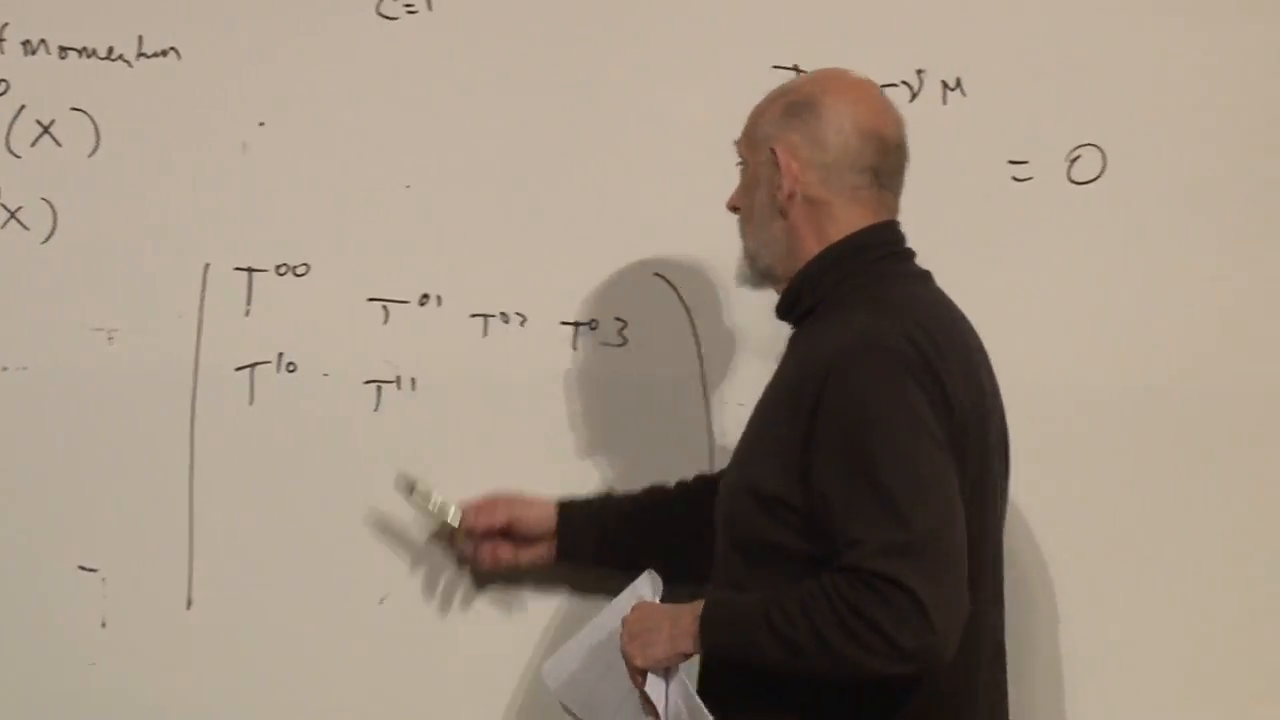
\includegraphics[width=0.84\textwidth]{lecture_09_figure_02.png}
\caption{Le tableau énergie-impulsion en cours d’élaboration au tableau. Le premier indice sélectionne l’énergie ou une composante de la quantité de mouvement ; le second sélectionne la densité ou le flux.}
\lectureframe{00:44:30}
\end{figure}

Le tableau complet est
\begin{equation}
 T^{\mu\nu}=
 \begin{pmatrix}
 T^{00}&T^{01}&T^{02}&T^{03}\\
 T^{10}&T^{11}&T^{12}&T^{13}\\
 T^{20}&T^{21}&T^{22}&T^{23}\\
 T^{30}&T^{31}&T^{32}&T^{33}
 \end{pmatrix}.
\end{equation}
Un autre théorème de la mécanique relativiste et de la théorie des champs implique que le tenseur énergie-impulsion est symétrique :
\begin{equation}
 T^{\mu\nu}=T^{\nu\mu}.
 \label{eq:stress-symmetry}
\end{equation}
En particulier, le flux d’énergie et la densité de quantité de mouvement sont les éléments non diagonaux correspondants, considérés de part et d’autre de la diagonale. La symétrie permet aussi d’écrire l’équation~\eqref{eq:stress-continuity} sous sa forme habituelle :
\begin{equation}
 D_\mu T^{\mu\nu}=0.
 \label{eq:stress-conservation}
\end{equation}

\begin{classroomqa}
\audiencequestion{Pourquoi le tenseur énergie-impulsion a-t-il gagné un indice supplémentaire, alors que le courant de charge n’en nécessitait qu’un ?}
\lecturerresponse{L’indice du courant distingue déjà la densité de la direction du flux. La charge n’a pas besoin d’une étiquette supplémentaire, car la charge conservée est un scalaire. L’énergie et les trois composantes de la quantité de mouvement sont elles-mêmes quatre composantes ; le premier indice précise donc quelle grandeur conservée est considérée, et le second indique s’il s’agit d’une densité ou d’un flux.
\lecturetimestamp{00:45:31--00:47:24}}
\end{classroomqa}

\begin{classroomqa}
\audiencequestion{La matrice \(T^{\mu\nu}\) entière est-elle symétrique, et pas seulement les éléments qui correspondent au flux d’énergie et à la densité de quantité de mouvement ?}
\lecturerresponse{Oui. La matrice entière est symétrique. La signification détaillée de ses éléments spatiaux, notamment la pression et les contraintes, sera développée plus loin.
\lecturetimestamp{00:47:32--00:47:54}}
\end{classroomqa}

La densité d’énergie n’était donc qu’un élément d’un objet plus vaste. La source de la gravitation ne peut pas être de façon cohérente \(T^{00}\) seule ; elle doit faire intervenir le tenseur entier.

\section{Une loi ne peut sélectionner une seule composante}

On peut voir pourquoi une équation tensorielle est nécessaire sans effectuer le moindre calcul de courbure. Supposons que \(A_i\) et \(B_i\) soient des vecteurs et qu’une loi proposée affirme seulement \(A_3=B_3\). Pour que cette égalité soit valable dans tout référentiel tourné, faisons tourner l’axe trois vers l’axe deux. La même loi affirme alors \(A_2=B_2\) ; une autre rotation donne \(A_1=B_1\). Une loi indépendante du référentiel était en réalité l’équation vectorielle
\begin{equation}
 A_i=B_i.
\end{equation}

Les transformations de Lorentz étendent le même raisonnement au temps. Pour que \(A^0=B^0\) soit valable dans tout référentiel inertiel, les transformations de Lorentz mélangent la composante temporelle aux composantes spatiales et imposent l’équation complète \(A^\mu=B^\mu\). Les bonnes lois relativistes égalent des tenseurs de même type.

L’aide-mémoire newtonien isolait \(T^{00}\), mais l’équation relativiste doit prendre la forme
\begin{equation}
 G_{\mu\nu}=8\pi G\,T_{\mu\nu},
 \label{eq:field-schematic}
\end{equation}
où le symbole \(G_{\mu\nu}\) n’est, au départ, qu’un symbole provisoire. Ses propriétés nécessaires sont maintenant claires :
\begin{enumerate}
 \item il doit s’agir d’un tenseur symétrique de rang deux ;
 \item il doit être construit à partir de la métrique, et non de la matière ;
 \item il doit contenir deux dérivées de la métrique ;
 \item sa divergence covariante doit s’annuler.
\end{enumerate}
La dernière condition découle de l’équation~\eqref{eq:stress-conservation}.

\section{À la recherche des tenseurs de courbure}

Les symboles de Christoffel contiennent une dérivée de la métrique :
\begin{equation}
 \Gamma^\sigma_{\tau\nu}
 =
 \frac12 g^{\sigma\delta}
 \left(
 \partial_\tau g_{\delta\nu}
 +\partial_\nu g_{\delta\tau}
 -\partial_\delta g_{\tau\nu}
 \right).
 \label{eq:christoffel}
\end{equation}
Ce ne sont pas des tenseurs ; ils ne peuvent donc pas, à eux seuls, fournir le membre de gauche. Le tenseur de courbure de Riemann est un tenseur :
\begin{equation}
 R^\rho{}_{\sigma\mu\nu}
 =
 \partial_\mu\Gamma^\rho_{\nu\sigma}
 -\partial_\nu\Gamma^\rho_{\mu\sigma}
 +\Gamma^\rho_{\mu\lambda}\Gamma^\lambda_{\nu\sigma}
 -\Gamma^\rho_{\nu\lambda}\Gamma^\lambda_{\mu\sigma}.
 \label{eq:riemann}
\end{equation}
Ses deux premiers termes contiennent des dérivées secondes de la métrique ; les deux derniers contiennent des produits de dérivées premières. C’est précisément l’ordre différentiel suggéré par l’équation newtonienne.

Le problème est la structure des indices. \(R^\rho{}_{\sigma\mu\nu}\) a quatre indices, tandis que \(T_{\mu\nu}\) en a deux. En contractant un indice supérieur et un indice inférieur convenablement choisis, on obtient le tenseur de Ricci,
\begin{equation}
 R_{\mu\nu}=R^\lambda{}_{\mu\lambda\nu}.
 \label{eq:ricci}
\end{equation}
Les autres contractions qui pourraient sembler possibles s’annulent à cause des symétries du tenseur de Riemann ou redonnent le même objet à un signe et une convention d’indices près. Le tenseur de Ricci est symétrique, mais il contient moins d’information que le tenseur de Riemann complet : il peut s’annuler alors que le tenseur de Riemann reste non nul.

\begin{classroomqa}
\audiencequestion{Peut-on simplement contracter deux indices inférieurs du tenseur de Riemann ? Une contraction ne nécessite-t-elle pas un indice covariant et un indice contravariant ?}
\lecturerresponse{Exactement. Il faut d’abord relever un indice à l’aide de la métrique inverse ; de façon équivalente, la contraction doit inclure \(g^{\mu\nu}\). Écrit sous la forme \(R^\lambda{}_{\mu\lambda\nu}\), le couple d’indices supérieur-inférieur requis est explicite.
\lecturetimestamp{01:00:09--01:00:33}}
\end{classroomqa}

En contractant encore une fois le tenseur de Ricci, on obtient le scalaire de courbure,
\begin{equation}
 R=g^{\mu\nu}R_{\mu\nu}.
 \label{eq:ricci-scalar}
\end{equation}
Multiplier ce scalaire par \(g_{\mu\nu}\) donne un autre tenseur symétrique de rang deux. Nous avons donc trouvé deux candidats naturels :
\begin{equation}
 R_{\mu\nu},
 \qquad
 g_{\mu\nu}R.
\end{equation}

\begin{figure}[htbp]
\centering
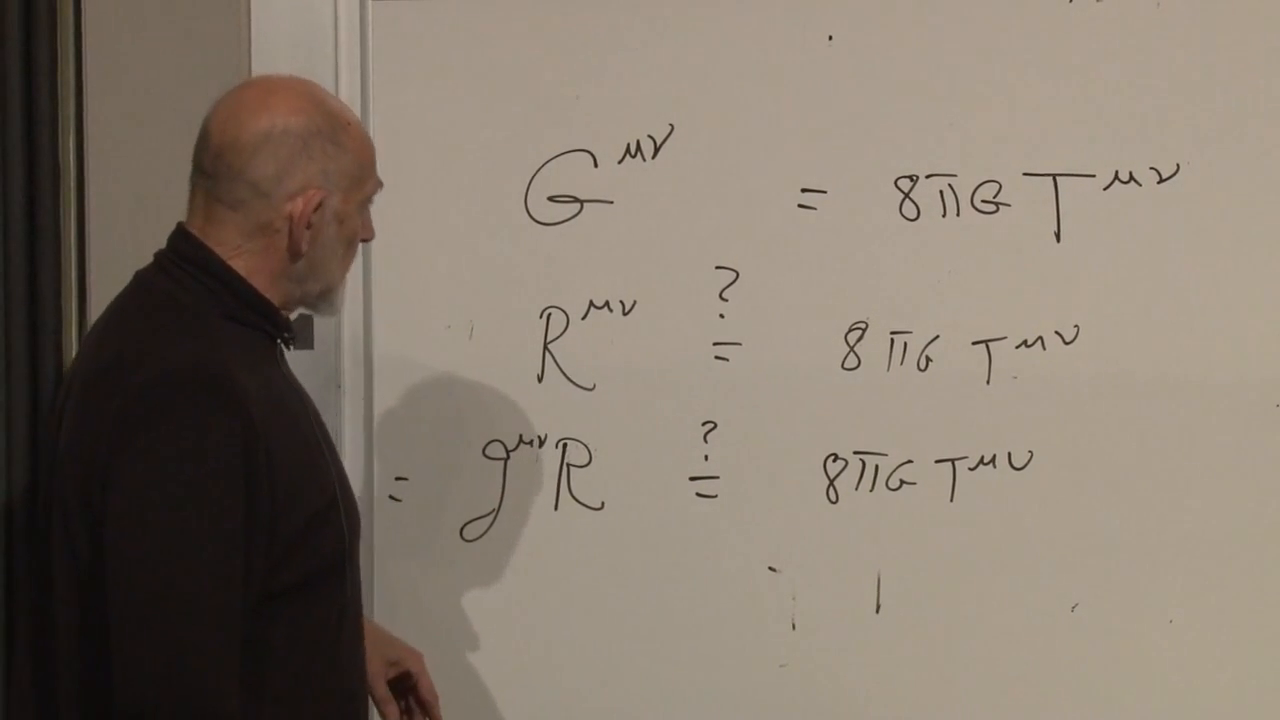
\includegraphics[width=0.78\textwidth]{lecture_09_figure_03.png}
\caption{Les deux tenseurs géométriques envisagés au tableau. À ce stade, leur rang et leur ordre différentiel conviennent tous deux ; chacun est donc accompagné d’un point d’interrogation.}
\lectureframe{01:04:56}
\end{figure}

Les deux possibilités envisagées sont
\begin{align}
 R_{\mu\nu}&\stackrel{?}{=}8\pi G\,T_{\mu\nu},\\
 g_{\mu\nu}R&\stackrel{?}{=}8\pi G\,T_{\mu\nu}.
\end{align}
Aucune ne doit être retenue au seul motif que ses indices conviennent. La conservation permet de les départager.

\section{Le test de la divergence}

Si l’équation~\eqref{eq:field-schematic} est correcte, alors
\begin{equation}
 D_\mu G^{\mu\nu}=0
\end{equation}
doit s’ensuivre identiquement, puisque \(D_\mu T^{\mu\nu}=0\). Commençons par le candidat faisant intervenir le scalaire de courbure. La règle du produit donne
\begin{equation}
 D_\mu\!\left(g^{\mu\nu}R\right)
 =
 \left(D_\mu g^{\mu\nu}\right)R
 +g^{\mu\nu}D_\mu R.
 \label{eq:product-rule}
\end{equation}

\begin{figure}[htbp]
\centering
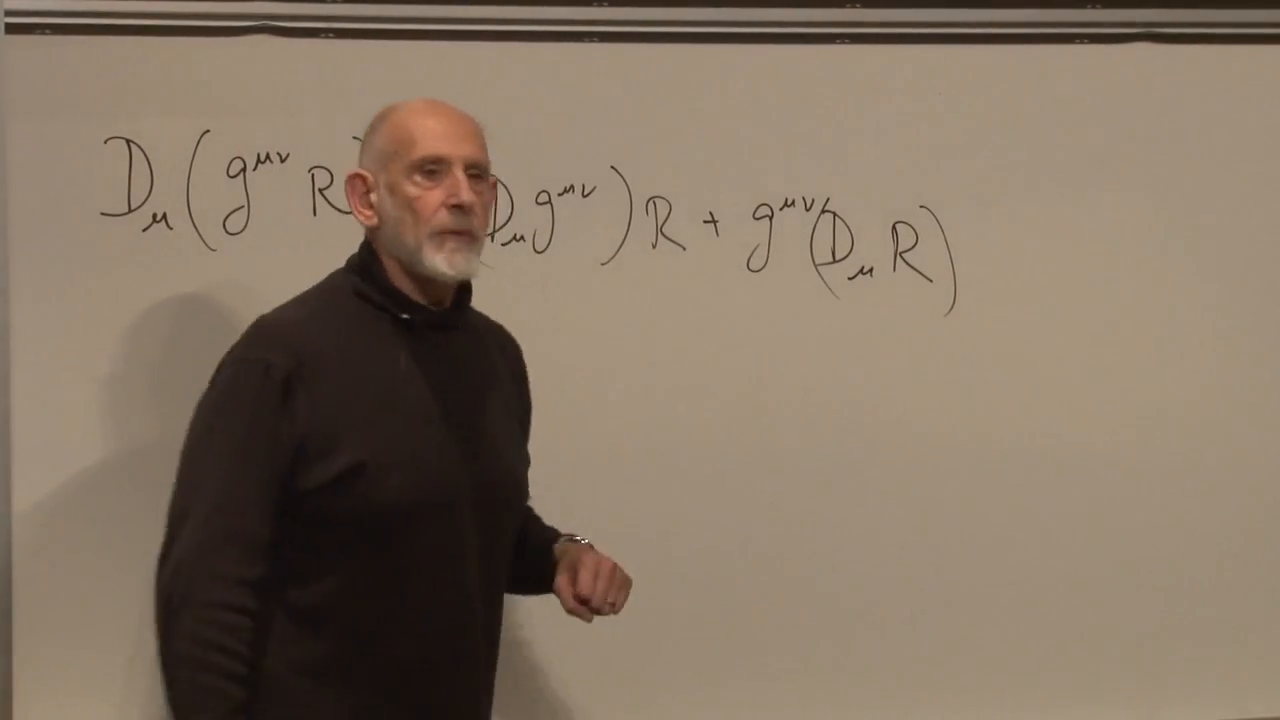
\includegraphics[width=0.84\textwidth]{lecture_09_figure_04.png}
\caption{Application de la règle du produit covariante à \(D_\mu(g^{\mu\nu}R)\).}
\lectureframe{01:07:12}
\end{figure}

La compatibilité métrique s’écrit
\begin{equation}
 D_\mu g^{\alpha\beta}=0.
 \label{eq:metric-compatibility}
\end{equation}
C’est une propriété géométrique indépendante de la connexion de Levi-Civita, et non une conséquence de la conservation de l’énergie-impulsion. Puisque \(R\) est un scalaire, \(D_\mu R=\partial_\mu R\). L’équation~\eqref{eq:product-rule} devient donc
\begin{equation}
 D_\mu(g^{\mu\nu}R)
 =g^{\mu\nu}\partial_\mu R
 =D^\nu R,
\end{equation}
ce qui n’est généralement pas nul. Le candidat \(g^{\mu\nu}R\) échoue.

Le calcul correspondant pour le tenseur de Ricci est un peu plus long. Il aboutit à l’identité de Bianchi contractée,
\begin{equation}
 D_\mu R^{\mu\nu}=\frac12 D^\nu R.
 \label{eq:contracted-bianchi}
\end{equation}
Le tenseur \(R^{\mu\nu}\) échoue donc lui aussi pris isolément. Mais les deux échecs sont dans le rapport précis qui permet une annulation :
\begin{equation}
 D_\mu\left(
 R^{\mu\nu}-\frac12 g^{\mu\nu}R
 \right)=0.
\end{equation}
On obtient ainsi le tenseur d’Einstein,
\begin{equation}
 \boxed{
 G_{\mu\nu}
 =
 R_{\mu\nu}-\frac12 g_{\mu\nu}R
 }.
 \label{eq:einstein-tensor}
\end{equation}

Dans le cadre des hypothèses retenues ici -- à savoir un tenseur local symétrique de rang deux, construit à partir de la métrique et ne contenant pas plus de deux dérivées --, cette combinaison est déterminée à un coefficient global près, avec la possibilité d’ajouter un terme métrique. Ce dernier correspond à la constante cosmologique, qui reviendra vers la fin du cours. Le coefficient devant l’équation~\eqref{eq:einstein-tensor} est fixé en imposant la limite newtonienne.

\begin{classroomqa}
\audiencequestion{Existe-t-il une façon plus directement physique d’obtenir l’équation de champ, plutôt que de proposer des candidats puis de les rejeter à l’aide de l’équation de continuité ?}
\lecturerresponse{La conservation locale est déjà un principe physique : l’énergie et la quantité de mouvement ne peuvent pas disparaître d’une région sans en traverser la frontière. Il existe aussi une dérivation plus condensée, fondée sur un principe d’action pour le champ gravitationnel. La variation de cette action produit la même équation, même si le calcul lui-même n’est pas bref.
\lecturetimestamp{01:17:14--01:18:41}}
\end{classroomqa}

\begin{classroomqa}
\audiencequestion{Un autre tenseur géométrique de rang deux pourrait-il satisfaire la même loi de conservation ? La réponse est-elle d’ordre physique ou mathématique, et Einstein l’aurait-il connue ?}
\lecturerresponse{Dans le cadre des hypothèses de cette construction, la classification est mathématique. Les objets de courbure disponibles avec deux dérivées proviennent du tenseur de Riemann ; les deux candidats de rang deux que nous venons d’examiner couvrent toutes les contractions pertinentes. Il faut néanmoins effectuer un calcul pour trouver la combinaison à divergence nulle. Les principes sont simples, mais gérer les indices et les signes demande du travail.
\lecturetimestamp{01:18:42--01:21:44}}
\end{classroomqa}

\section{L’équation de champ et sa limite newtonienne}

L’équation de champ s’écrit maintenant
\begin{equation}
 \boxed{
 R_{\mu\nu}-\frac12 g_{\mu\nu}R
 =
 8\pi G\,T_{\mu\nu}
 }.
 \label{eq:einstein-equation}
\end{equation}
Le membre de gauche est géométrique ; celui de droite décrit la matière, le rayonnement et leurs flux. Leurs divergences covariantes s’annulent simultanément.

Le facteur \(8\pi G\) n’est pas déterminé par l’argument de divergence. On le détermine en considérant un champ gravitationnel faible et lentement variable, produit par de la matière se déplaçant lentement, puis en exigeant que la composante temporelle reproduise l’équation de Poisson. Dans ce régime, \(T_{00}\simeq\rho\), tandis que les autres composantes sont atténuées par des puissances de \(v/c\). Le membre géométrique se réduit à la structure en dérivées secondes anticipée dans l’équation~\eqref{eq:weak-mnemonic}. L’accord donne exactement la normalisation de l’équation~\eqref{eq:einstein-equation}.

Cette limite explique aussi pourquoi la gravitation newtonienne semble n’avoir pour source que la densité de masse. Dans la théorie complète, chaque composante de \(T_{\mu\nu}\) contribue à la gravitation : la densité d’énergie, le flux d’énergie, la densité de quantité de mouvement, la pression et le cisaillement. Pour la matière ordinaire non relativiste, l’énergie de masse domine. Dans la matière relativiste, le rayonnement ou les systèmes soumis à une forte pression, on ne peut pas négliger les autres composantes.

Le cheminement historique ne fut pas une intuition immédiate et sans effort. Le tenseur de Ricci paraît être le premier candidat évident, et le terme supplémentaire \(-\tfrac12g_{\mu\nu}R\) assure la compatibilité avec la conservation locale. Une fois la structure tensorielle fixée, la limite newtonienne fournit la normalisation.

\section{Ce que la contraction laisse de côté}

\begin{classroomqa}
\audiencequestion{Lorsque les quatre indices du tenseur de Riemann sont contractés pour n’en garder que deux, l’information écartée a-t-elle un contenu physique ?}
\lecturerresponse{Oui. Le tenseur de Ricci ne contient pas toute la courbure de l’espace-temps. Les champs gravitationnels sans source en fournissent les exemples les plus nets : le tenseur de Ricci peut s’annuler alors que la courbure de marée et les ondes gravitationnelles subsistent. La contraction conserve la partie directement liée à l’équation locale de la source, mais pas tous les degrés de liberté du champ gravitationnel.
\lecturetimestamp{01:21:57--01:23:10}}
\end{classroomqa}

L’analogie avec l’électromagnétisme est utile. Les équations de Maxwell admettent des ondes dans une région dépourvue de charge et de courant. De même, l’équation d’Einstein admet une géométrie non triviale dans une région où \(T_{\mu\nu}=0\). Dérivons maintenant l’équation plus simple qui s’y applique.

\section{Le vide signifie Ricci plat, et non plat}

Posons
\begin{equation}
 T_{\mu\nu}=0.
\end{equation}
L’équation~\eqref{eq:einstein-equation} donne alors
\begin{equation}
 R_{\mu\nu}-\frac12g_{\mu\nu}R=0.
 \label{eq:vacuum-einstein}
\end{equation}
Contractons avec \(g^{\mu\nu}\). Comme
\begin{equation}
 g^{\mu\nu}g_{\mu\nu}
 =\delta^\mu{}_\mu=4
\end{equation}
dans un espace-temps à quatre dimensions, la trace est
\begin{equation}
 R-\frac12(4)R=-R=0.
\end{equation}
Par conséquent,
\begin{equation}
 R=0,
 \qquad
 R_{\mu\nu}=0.
 \label{eq:ricci-flat}
\end{equation}
L’équation de champ dans le vide impose que le tenseur de Ricci soit nul.

Il est essentiel de ne pas remplacer les mots \emph{Ricci plat} par \emph{plat}.
L’extérieur de Schwarzschild ne contient aucune matière en dehors de la singularité centrale, et il satisfait à \(R_{\mu\nu}=0\). Pourtant, son tenseur de Riemann est non nul et les forces de marée sont bien réelles. On peut vérifier que le tenseur de Ricci est nul en calculant à la main tous les symboles de Christoffel et toutes les composantes de courbure, au prix d’un calcul fastidieux, ou en confiant ces calculs à un système de calcul symbolique. À la singularité, les expressions classiques divergent ; partout ailleurs, l’équation du vide est vérifiée.

Les ondes gravitationnelles en fournissent un second exemple. Elles peuvent se propager dans une région sans source tout en transportant une véritable déformation de l’espace-temps. Ainsi,
\begin{equation}
 R_{\mu\nu}=0
 \quad\not\Rightarrow\quad
 R^\rho{}_{\sigma\mu\nu}=0.
\end{equation}

\section{Conserver la source : l’équation de la trace}

Le cours est sur le point de s’achever sur le résultat concernant le vide, mais une personne dans le public demande de refaire la contraction sans éliminer la source.

\begin{classroomqa}
\audiencequestion{Qu’obtient-on si l’on effectue la même contraction en laissant \(T_{\mu\nu}\) dans l’équation ?}
\lecturerresponse{La trace relie directement le scalaire de courbure à la trace du tenseur énergie-impulsion ; en réinjectant cette relation dans l’équation, on obtient une forme équivalente de l’équation de champ faisant intervenir le tenseur de Ricci.
\lecturetimestamp{01:29:28--01:32:20}}
\end{classroomqa}

Définissons
\begin{equation}
 T=g^{\mu\nu}T_{\mu\nu}.
\end{equation}
La trace de l’équation~\eqref{eq:einstein-equation} donne
\begin{align}
 R-\frac12(4)R&=8\pi G\,T,\\
 -R&=8\pi G\,T,
\end{align}
par conséquent,
\begin{equation}
 \boxed{R=-8\pi G\,T}.
 \label{eq:trace-relation}
\end{equation}
En reportant ce résultat dans l’équation de champ, on obtient
\begin{equation}
 \boxed{
 R_{\mu\nu}
 =
 8\pi G
 \left(
 T_{\mu\nu}-\frac12g_{\mu\nu}T
 \right)
 }.
 \label{eq:ricci-form}
\end{equation}

\begin{figure}[htbp]
\centering
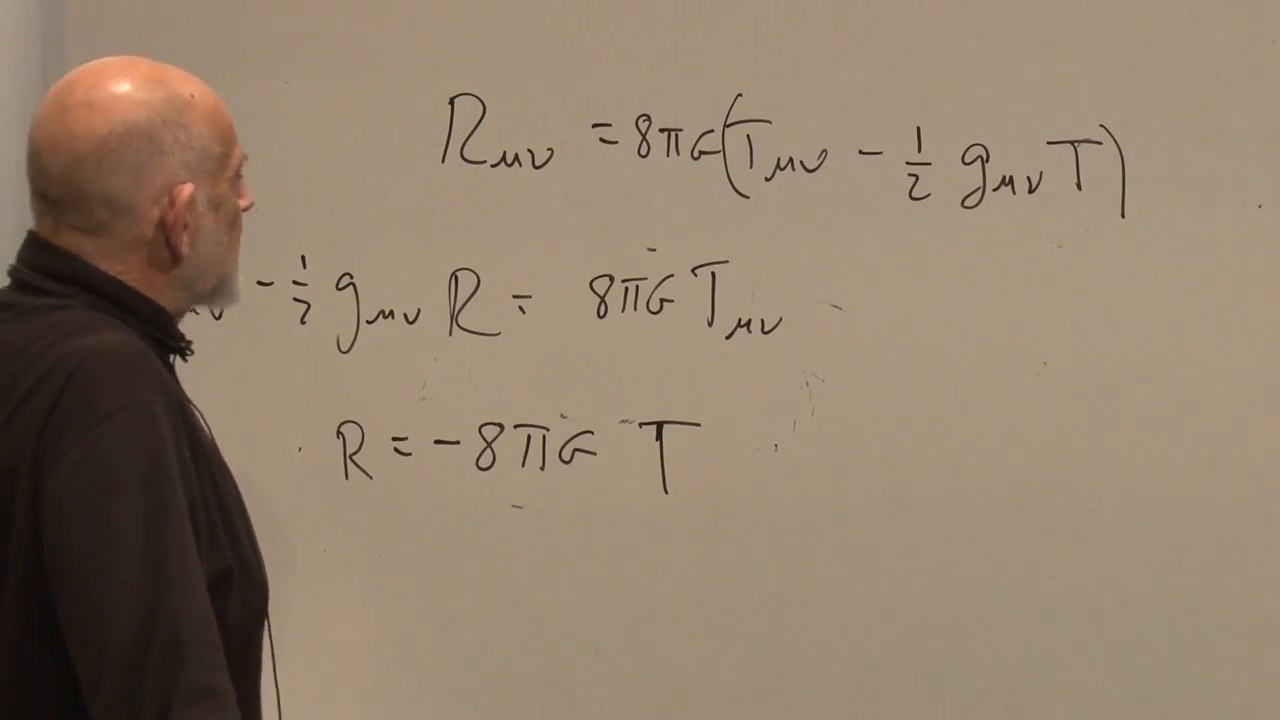
\includegraphics[width=0.82\textwidth]{lecture_09_figure_05.png}
\caption{La relation de trace et la forme équivalente de l’équation d’Einstein faisant intervenir le tenseur de Ricci.}
\lectureframe{01:32:25}
\end{figure}

\begin{classroomqa}
\audiencequestion{Le scalaire \(T\) a-t-il une signification physique ?}
\lecturerresponse{C’est la trace du tenseur énergie-impulsion. Elle s’annule pour le rayonnement électromagnétique ; il en va de même pour un gaz parfait de particules sans masse, comme les photons. La matière massive a généralement une trace non nulle. Par l’intermédiaire de l’équation~\eqref{eq:trace-relation}, cette trace détermine le scalaire de courbure.
\lecturetimestamp{01:32:20--01:33:12}}
\end{classroomqa}

\section{Quelle part de la courbure le tenseur de Ricci retient-il ?}

\begin{classroomqa}
\audiencequestion{Existe-t-il une représentation physique ou géométrique simple du tenseur de Ricci et du scalaire de Ricci, comparable au transport parallèle autour d’une petite boucle pour le tenseur de Riemann ?}
\lecturerresponse{Aucune représentation aussi transparente n’est proposée ici. Le tenseur de Riemann décrit directement la rotation résultant du transport autour d’une petite boucle. Ses contractions sont plus simples algébriquement, mais il est plus difficile de visualiser leur signification géométrique individuelle. Mieux vaut ne pas inventer une représentation trompeuse sous prétexte qu’elle serait commode.
\lecturetimestamp{01:33:14--01:34:13}}
\end{classroomqa}

La quantité d’information perdue lors de la contraction dépend de la dimension. En quatre dimensions, le tenseur de Riemann contient des informations sur la courbure absentes du tenseur de Ricci. En trois dimensions, le tenseur de Riemann est déterminé par le tenseur de Ricci. En deux dimensions, le scalaire de courbure contient toute l’information indépendante sur la courbure. La gravitation en quatre dimensions admet donc des degrés de liberté de courbure sans source, invisibles dans \(R_{\mu\nu}\).

\begin{classroomqa}
\audiencequestion{Si des tenseurs de Riemann différents peuvent avoir le même tenseur de Ricci, comment l’information manquante se manifeste-t-elle physiquement ?}
\lecturerresponse{Une source donnée ne spécifie pas à elle seule toutes les configurations gravitationnelles possibles. Les données aux limites et les données initiales peuvent inclure un rayonnement gravitationnel. Dans l’approximation de champ faible, on peut imaginer partir d’une solution avec source et y ajouter une onde gravitationnelle libre. La théorie non linéaire complète n’autorise pas une superposition arbitraire, mais cet exemple identifie correctement l’information manquante : une courbure qui se propage et n’est pas déterminée localement par \(T_{\mu\nu}\).
\lecturetimestamp{01:37:05--01:38:59}}
\end{classroomqa}

Deux exemples de vide s’accordent maintenant. La géométrie de Schwarzschild présente une courbure de marée à l’extérieur d’une masse. Une onde gravitationnelle transporte une courbure qui se propage librement. Chacune peut satisfaire à \(R_{\mu\nu}=0\) tout en restant non plate.

\section{La constante cosmologique}

\begin{classroomqa}
\audiencequestion{N’y a-t-il pas de facteur d’ajustement supplémentaire, comme une constante cosmologique ?}
\lecturerresponse{Une constante cosmologique est possible. On peut l’écrire du côté géométrique sous la forme d’une constante multipliée par \(g_{\mu\nu}\), ou la déplacer à droite et l’interpréter comme une contribution du vide au tenseur énergie-impulsion. Ces deux descriptions sont la même équation, avec une répartition différente des termes.
\lecturetimestamp{01:39:01--01:40:44}}
\end{classroomqa}

Avec une constante cosmologique, une convention courante consiste à écrire
\begin{equation}
 G_{\mu\nu}+\Lambda g_{\mu\nu}
 =
 8\pi G\,T_{\mu\nu}.
\end{equation}
En déplaçant le terme supplémentaire vers la droite, on définit un tenseur effectif des contraintes du vide,
\begin{equation}
 T_{\mu\nu}^{(\Lambda)}
 =
 -\frac{\Lambda}{8\pi G}g_{\mu\nu}.
\end{equation}
Comme la compatibilité métrique donne \(D_\mu g^{\mu\nu}=0\), le terme supplémentaire est automatiquement compatible avec la loi de conservation. C’est le terme métrique laissé en suspens dans l’affirmation d’unicité précédente.

\section{Mercure et le calcul en champ faible}

\begin{classroomqa}
\audiencequestion{Einstein a-t-il utilisé cette équation pour calculer l’orbite de Mercure, et où peut-on voir comment ce calcul a été effectué ?}
\lecturerresponse{Einstein a travaillé avant que Schwarzschild ne fournisse la solution exacte ; il a plutôt utilisé une approximation à grande distance suffisamment précise du champ extérieur du Soleil. Le rayon du Soleil et l’orbite de Mercure sont très grands par rapport au rayon de Schwarzschild du Soleil, de sorte que les corrections relativistes sont faibles. Il pouvait partir d’une orbite képlérienne et calculer la correction par perturbation. Peu après, Schwarzschild a obtenu la solution extérieure exacte, ce qui a rendu le même calcul systématique.
\lecturetimestamp{01:40:46--01:43:48}}
\end{classroomqa}

La théorie des perturbations consiste exactement en ceci : partir d’un problème déjà résolu, puis calculer l’effet d’une petite correction. La force newtonienne en raison inverse du carré de la distance produit des ellipses képlériennes fermées. La relativité générale ajoute une petite déviation à l’équation radiale newtonienne ; l’ellipse ne se referme donc pas après une révolution et son périhélie avance.

Le cours s’achève sur le caractère singulier des orbites fermées sous l’action d’une force centrale. La force en raison inverse du carré de la distance est exceptionnelle en ce qu’elle produit des orbites képlériennes fermées, sans précession. Plus généralement, le théorème de Bertrand désigne également l’oscillateur harmonique isotrope comme l’autre potentiel central pour lequel toutes les orbites liées sont fermées. La faible correction relativiste supprime cette dégénérescence newtonienne et fait de la précession de Mercure une signature observable de l’équation de champ établie dans ce chapitre.
\graphicspath{{../../../generated_course_notes/core/general_relativity/2012_fall_theoretical_minimum/chapters/lecture_10/}{../../../generated_course_notes/core/general_relativity/2012_fall_theoretical_minimum/figures/}{../../../generated_course_notes/core/general_relativity/2012_fall_theoretical_minimum/assets/}}
\chapter{Champs faibles, ondes gravitationnelles et principe de l’action}

Les équations exactes de la relativité générale sont non linéaires, et leur expression en composantes peut devenir redoutable avant même qu’on ait résolu un seul problème physique. Pour cette dernière leçon du cours, mieux vaut distinguer les principes des calculs. Nous examinerons ce que deviennent les équations d’Einstein lorsque le champ gravitationnel est faible, nous identifierons les ondes que contient cette approximation, puis nous verrons comment les équations complètes du champ s’inscrivent dans un principe d’action remarquablement compact.

Trois questions structurent la discussion. Que signifie un champ gravitationnel faible ? Pourquoi la théorie faible est-elle linéaire alors que la théorie exacte ne l’est pas ? Et quels effets physiques permettent de distinguer une onde gravitationnelle d’une simple ondulation des coordonnées ?

\section{Petite perturbation d’une géométrie d’équilibre}

La faiblesse est une méthode d’approximation. Si une perturbation sans dimension est de l’ordre de \(\epsilon\ll1\), son carré est de l’ordre de \(\epsilon^2\), et un calcul au premier ordre néglige systématiquement ce dernier terme. L’exemple classique est celui d’un système mécanique qui effectue de petites oscillations autour de l’équilibre. Ses équations exactes peuvent être non linéaires, mais des oscillations suffisamment petites obéissent à des équations linéaires.

En gravitation, l’état d’équilibre sera l’espace-temps plat et vide. Partons de l’équation du vide d’Einstein,
\begin{equation}
 R_{\mu\nu}-\frac12 g_{\mu\nu}R=0.
 \label{eq:l10-vacuum-einstein}
\end{equation}
Sa trace en quatre dimensions donne
\begin{equation}
 g^{\mu\nu}
 \left(R_{\mu\nu}-\frac12 g_{\mu\nu}R\right)
 =R-2R=-R=0,
\end{equation}
L’équation du vide est donc équivalente à
\begin{equation}
 R_{\mu\nu}=0.
 \label{eq:l10-ricci-flat}
\end{equation}

\begin{figure}[htbp]
\centering
\includegraphics[width=0.68\textwidth]{lecture_10_figure_02.png}
\caption{L’équation du vide \(R_{\mu\nu}=0\), isolée au début de l’argument sur les champs faibles.}
\lectureframe{00:03:11}
\end{figure}

Ici, l’équilibre désigne une solution sans source et indépendante du temps. L’espace-temps plat est la solution de ce type la plus simple. Une précision est essentielle : la platitude ne signifie pas que les composantes de la métrique soient égales à une matrice particulière dans tout système de coordonnées. Elle signifie qu’on peut choisir des coordonnées inertielles dans lesquelles
\begin{equation}
 g_{\mu\nu}=\eta_{\mu\nu}.
\end{equation}
Cette distinction entre une géométrie et les coordonnées qui servent à la décrire deviendra bientôt la subtilité centrale.

Imaginons maintenant une source violente, telle qu’un système binaire compact. Son champ proche peut être intense, mais loin de la source, la perturbation se propage et devient petite. Dans un système de coordonnées adapté, la métrique peut alors s’écrire
\begin{equation}
 g_{\mu\nu}(x)=\eta_{\mu\nu}+h_{\mu\nu}(x),
 \qquad |h_{\mu\nu}|\ll1.
 \label{eq:weak-split}
\end{equation}
La perturbation \(h_{\mu\nu}\) peut dépendre des quatre coordonnées de l’espace-temps. La faiblesse signifie que l’on néglige les termes d’ordre supérieur au premier.

\section{Ce qui subsiste au premier ordre}

Le tenseur de Ricci complet est trop long pour être utile à ce stade. Sa structure suffit. Les symboles de Christoffel contiennent la métrique inverse et une dérivée de la métrique, tandis que la courbure contient une dérivée d’un symbole de Christoffel et un produit de deux symboles de Christoffel :
\begin{equation}
 \Gamma\sim\frac12 g^{-1}\partial g,
 \qquad
 R\sim\partial\Gamma+\Gamma\Gamma.
 \label{eq:curvature-skeleton}
\end{equation}

\begin{figure}[htbp]
\centering
\includegraphics[width=0.84\textwidth]{lecture_10_figure_03.png}
\caption{La décomposition en champ faible et la construction schématique
\(R\sim\partial\Gamma+\Gamma\Gamma\). La notation fait apparaître les ordres en
\(h\) sans développer chaque indice.}
\lectureframe{00:10:17}
\end{figure}

La métrique inverse se déduit de
\(g^{\mu\alpha}g_{\alpha\nu}=\delta^\mu{}_\nu\). Au premier ordre,
\begin{equation}
 g^{\mu\nu}=\eta^{\mu\nu}-h^{\mu\nu}+O(h^2),
 \label{eq:inverse-weak}
\end{equation}
où les indices de \(h\) sont relevés à l’aide de la métrique de fond. Dans des coordonnées inertielles, la métrique de fond est constante,
\begin{equation}
 \partial_\alpha\eta_{\mu\nu}=0,
\end{equation}
et par conséquent
\begin{equation}
 \partial_\alpha g_{\mu\nu}
 =\partial_\alpha h_{\mu\nu}.
\end{equation}
On obtient donc
\begin{equation}
\begin{aligned}
 \Gamma&=O(\partial h),\\
 R_{\mu\nu}
 &=O(\partial\partial h)+O\bigl((\partial h)^2\bigr)\\
 &\quad+O(h\,\partial\partial h).
\end{aligned}
 \label{eq:ricci-orders}
\end{equation}

\begin{figure}[htbp]
\centering
\includegraphics[width=0.84\textwidth]{lecture_10_figure_04.png}
\caption{Le développement de la métrique inverse au tableau et l’observation que
\(\partial\eta=0\). Seules les dérivées de \(h_{\mu\nu}\) subsistent au premier ordre.}
\lectureframe{00:11:55}
\end{figure}

Les deux derniers termes de l’équation~\eqref{eq:ricci-orders} sont quadratiques en la perturbation et sont omis. Les équations du vide sont donc des équations linéaires faisant intervenir les dérivées secondes de \(h_{\mu\nu}\). C’est tout ce que signifie la linéarisation. Cela ne signifie pas que la théorie exacte d’Einstein soit linéaire.

\begin{classroomqa}
\audiencequestion{Le tenseur de courbure a quatre indices, tandis que le tenseur de Ricci en a deux. Si deux dérivées portent déjà des indices et que \(h_{\mu\nu}\) en porte deux autres, comment s’effectue le comptage des indices ?}
\lecturerresponse{On obtient le tenseur de Ricci en contractant une paire d’indices du tenseur de courbure. La métrique utilisée pour cette contraction laisse deux indices libres, précisément ceux de \(R_{\mu\nu}\). La forme symbolique \(\partial\partial h\) ne fait pas apparaître ces contractions : elle indique l’ordre des termes, et non une formule complète avec indices.
\lecturetimestamp{00:18:45--00:19:53}}
\end{classroomqa}

\begin{classroomqa}
\audiencequestion{La contraction avec la métrique inverse introduit-elle des termes tels que \(h\,\partial^2h\), et si oui, pourquoi peut-on les négliger ?}
\lecturerresponse{C’est le cas. En remplaçant \(g^{-1}\) par
\(\eta^{-1}-h+\cdots\), on obtient le terme linéaire
\(\eta^{-1}\partial^2h\) ainsi que des corrections contenant une deuxième puissance de \(h\). Ces dernières sont quadratiques. La même règle permet d’écarter
\(h\,\partial h\), \(h\,\partial^2h\) et
\((\partial h)^2\). Ne conserver qu’une seule puissance de la perturbation, c’est précisément faire l’approximation considérée.
\lecturetimestamp{00:19:55--00:21:14}}
\end{classroomqa}

\section{Pourquoi les équations prennent la forme d’ondes}

Des équations de champ faisant intervenir des dérivées secondes suggèrent naturellement une propagation ondulatoire. Pour une fonction scalaire se propageant selon l’axe \(z\), l’équation type est
\begin{equation}
 \left(\partial_t^2-\partial_z^2\right)\phi=0,
\end{equation}
dont les solutions comprennent des profils arbitraires se propageant vers la droite ou vers la gauche,
\begin{equation}
 \phi(z,t)=f(z-t)+g(z+t).
\end{equation}
En trois dimensions d’espace, la même équation s’écrit
\begin{equation}
 \left(\partial_t^2-\nabla^2\right)\phi=0.
\end{equation}
Sa linéarité autorise la superposition : la somme de deux solutions est encore une solution.

La gravitation n’est pas un champ scalaire. La perturbation possède des composantes tensorielles, et l’équation \(R_{\mu\nu}=0\) semble d’abord fournir de nombreuses équations pour ces composantes. Elles ne sont pas toutes indépendantes : certaines sont des contraintes, d’autres traduisent la liberté de choix des coordonnées. L’analogie est celle de la théorie de Maxwell, où un ensemble d’équations de champ ne laisse finalement subsister que les ondes transversales physiques.

Une fois imposées des conditions de coordonnées adaptées, les composantes radiatives obéissent à une équation d’onde ordinaire,
\begin{equation}
 \Box h_{\mu\nu}=0,
 \qquad
 \Box=\eta^{\alpha\beta}\partial_\alpha\partial_\beta.
 \label{eq:linear-wave}
\end{equation}
Les signes précis dans \(\Box\) dépendent de la convention de signature ; le contenu, lui, ne change pas. Les perturbations se propagent sur le cône de lumière.

\section{Les ondulations des coordonnées ne sont pas des ondes gravitationnelles}

Avant de considérer toute solution des équations linéarisées comme une onde physique, revenons à la réserve concernant les coordonnées. On peut décrire l’espace plat avec des lignes de coordonnées courbes. Les composantes de la métrique diffèrent alors de leurs valeurs cartésiennes, même si la courbure reste nulle.

Le tableau lui-même en fournit un exemple. Traçons des coordonnées cartésiennes sur sa surface plane et écrivons
\begin{equation}
 ds^2=\delta_{mn}\,dx'^m dx'^n.
\end{equation}
Puis attribuons aux mêmes points des coordonnées légèrement ondulées,
\begin{equation}
 x'^m=x^m+f^m(x).
 \label{eq:small-coordinate-change}
\end{equation}
Les différentielles deviennent
\begin{equation}
 dx'^m=dx^m+\partial_n f^m\,dx^n.
\end{equation}
En substituant ces expressions dans l’élément de ligne et en ne conservant que le premier ordre en \(f\), on obtient
\begin{align}
 ds^2
 &=\delta_{mn}dx^m dx^n\\
 &\quad+\left(\partial_m f_n+\partial_n f_m\right)dx^m dx^n
 +O(f^2).
\end{align}
Ainsi, une perturbation apparente de la forme
\begin{equation}
 h_{mn}=\partial_m f_n+\partial_n f_m
 \label{eq:pure-gauge}
\end{equation}
peut ne décrire aucune nouvelle géométrie. Il s’agit de l’espace plat en coordonnées ondulées.

\begin{figure}[htbp]
\centering
\includegraphics[width=0.84\textwidth]{lecture_10_figure_05.png}
\caption{Le calcul des ondulations de coordonnées au tableau. Un léger changement de coordonnées induit un \(h_{mn}\) d’apparence faible, même si la surface du tableau reste plate.}
\lectureframe{00:27:54}
\end{figure}

L’équation~\eqref{eq:pure-gauge} est la forme linéarisée de la liberté de choix des coordonnées, ou liberté de jauge. Il faut imposer des conditions supplémentaires pour éliminer ces fausses perturbations. L’algèbre détaillée de la jauge n’est pas développée ici. Son rôle est toutefois essentiel : elle élimine les changements de description tout en préservant les changements de courbure. Une fois prises en compte la liberté de choix des coordonnées et les équations de contrainte, le contenu physique se réduit à deux polarisations indépendantes de l’onde.

\begin{figure}[htbp]
\centering
\begin{tikzpicture}[scale=0.86]
\begin{scope}
\draw[->] (-0.2,0) -- (3.3,0) node[right] {$x$};
\draw[->] (0,-0.2) -- (0,3.3) node[above] {$y$};
\foreach \u in {0.6,1.2,1.8,2.4,3.0}{
  \draw (\u,0) -- (\u,3.0);
  \draw (0,\u) -- (3.0,\u);
}
\node at (1.5,-0.55) {Cartesian labels};
\end{scope}
\begin{scope}[xshift=5.3cm]
\draw[->] (-0.2,0) -- (3.4,0) node[right] {$x$};
\draw[->] (0,-0.2) -- (0,3.3) node[above] {$y$};
\foreach \u in {0.6,1.2,1.8,2.4,3.0}{
  \draw[decorate,decoration={snake,amplitude=0.09cm,segment length=0.7cm}]
    (\u,0) -- (\u,3.0);
  \draw[decorate,decoration={snake,amplitude=0.09cm,segment length=0.7cm}]
    (0,\u) -- (3.0,\u);
}
\node at (1.5,-0.55) {wiggly labels};
\end{scope}
\end{tikzpicture}
\caption{La géométrie reste plate tandis que le réseau de coordonnées change. Les seules composantes de la métrique ne permettent pas de décider si une perturbation est physique.}
\end{figure}

\section{Une onde se propageant selon l’axe z}

Choisissons une onde plane se propageant dans le sens positif de \(z\). Sa phase peut s’écrire
\begin{equation}
 k(z-t),
\end{equation}
Une composante représentative prend donc la forme
\begin{equation}
 h_{\mu\nu}(z,t)
 =h_{\mu\nu}^{(0)}\sin k(z-t).
 \label{eq:plane-wave}
\end{equation}
Les surfaces de phase constante satisfont \(z-t=\text{constant}\) ; la vitesse de propagation est donc celle de la lumière.

Dans une description transverse et sans trace, les composantes comportant un indice temporel ou un indice \(z\) s’annulent :
\begin{equation}
 h_{0\mu}=0,
 \qquad
 h_{z\mu}=0.
 \label{eq:tt-transverse}
\end{equation}
Seul subsiste le bloc \(x\)-\(y\). Il est symétrique et sans trace,
\begin{equation}
 h_{xy}=h_{yx},
 \qquad
 h_{xx}+h_{yy}=0.
 \label{eq:tt-trace}
\end{equation}

\begin{figure}[htbp]
\centering
\includegraphics[width=0.84\textwidth]{lecture_10_figure_06.png}
\caption{Une onde se propageant selon \(z\), représentée par un empilement de plans transversaux. Les amplitudes restantes dans le plan \(x\)-\(y\) obéissent à la condition
\(h_{xx}+h_{yy}=0\).}
\lectureframe{00:43:36}
\end{figure}

Il existe donc deux configurations indépendantes. Pour
\(i,j\in\{x,y\}\), on peut les représenter ainsi :
\begin{equation}
 h^{\mathrm{TT}}_{ij}(z,t)
 =
 \begin{pmatrix}
 h_+ & h_\times\\
 h_\times & -h_+
 \end{pmatrix}
 \sin k(z-t).
 \label{eq:polarization-matrix}
\end{equation}
La configuration diagonale est appelée polarisation plus. Celle dont les composantes sont hors diagonale est appelée polarisation croix. Une rotation des axes transversaux de \(45^\circ\) transforme l’une en l’autre, et toute onde polarisée linéairement est une superposition des deux. Cette théorie ne comporte pas d’autres polarisations indépendantes.

\begin{figure}[htbp]
\centering
\begin{tikzpicture}[scale=0.88]
\begin{scope}
\draw[->] (-1.8,0) -- (1.8,0) node[right] {$x$};
\draw[->] (0,-1.7) -- (0,1.7) node[above] {$y$};
\draw[dashed] (0,0) circle (1.0);
\draw[thick] (0,0) ellipse (1.35 and 0.65);
\node at (0,-2.05) {plus polarization};
\end{scope}
\begin{scope}[xshift=5.0cm]
\draw[->] (-1.8,0) -- (1.8,0) node[right] {$x$};
\draw[->] (0,-1.7) -- (0,1.7) node[above] {$y$};
\draw[dashed] (0,0) circle (1.0);
\draw[thick,rotate=45] (0,0) ellipse (1.35 and 0.65);
\node at (0,-2.05) {cross polarization};
\end{scope}
\end{tikzpicture}
\caption{Durant une demi-période, une direction transverse s’étire tandis que la direction perpendiculaire se comprime. Une demi-période plus tard, la déformation s’inverse.}
\end{figure}

\section{Des composantes de la métrique à la déformation physique}

Fixons \(z\) et \(t\), puis examinons le plan transverse. Pour une onde purement polarisée plus,
\begin{equation}
 ds_\perp^2
 =(1+h_{xx})\,dx^2+(1-h_{xx})\,dy^2.
 \label{eq:transverse-distance}
\end{equation}
Lorsque \(h_{xx}>0\), un intervalle de coordonnées fixe selon \(x\) a une longueur propre légèrement plus grande, tandis que l’intervalle correspondant selon \(y\) a une longueur légèrement plus petite. Une demi-période plus tard, \(h_{xx}\) change de signe et les rôles s’inversent. Un carré s’étire tour à tour horizontalement et se comprime verticalement, puis se comprime horizontalement et s’étire verticalement. Pour la polarisation croix, la même alternance se produit selon des axes tournés de \(45^\circ\).

Au premier ordre, la longueur initiale \(L\) d’un bras varie de
\begin{equation}
 \frac{\Delta L}{L}\simeq\frac12 h_{ij}n^i n^j,
 \label{eq:fractional-strain}
\end{equation}
où \(\mathbf n\) est dirigé le long du bras. Cette formule traduit la perturbation de la métrique en la déformation relative sans dimension mesurée par un détecteur.

\begin{classroomqa}\audiencequestion{Une règle graduée est maintenue par les forces électromagnétiques et sa longueur au repos ne varie pas simplement avec les coordonnées. Ne faudrait-il pas plutôt représenter des masses d’épreuve librement séparées ?}\lecturerresponse{La distinction est importante. Une tige réelle possède une élasticité : le champ de marée y engendre donc des contraintes internes. Une tige d’acier et une tige de bois réagiront généralement différemment. Des masses d’épreuve suspendues librement évitent cette réponse élastique particulière et révèlent plus directement l’accélération relative. Dans les deux cas, l’onde qui passe ne fait pas que réattribuer des étiquettes aux points. Sa courbure variable dans le temps produit un effet physique.
\lecturetimestamp{00:47:23--00:48:48}}
\end{classroomqa}

La formulation locale précise est celle de la déviation géodésique. Pour des particules voisines en chute libre, séparées par \(\xi^i\),
\begin{equation}
 \frac{d^2\xi^i}{dt^2}
 =-R^i{}_{0j0}\,\xi^j.
 \label{eq:geodesic-deviation}
\end{equation}
Dans une onde faible transverse et sans trace,
\begin{equation}
 R_{0i0j}=-\frac12\ddot h^{\mathrm{TT}}_{ij},
 \label{eq:tidal-curvature}
\end{equation}
la métrique oscillante engendre donc une accélération de marée alternée. C’est pourquoi une onde dépendant du temps ne peut pas être écartée comme un choix statique de règles de mesure. Sa courbure n’est pas nulle.

\begin{classroomqa}\audiencequestion{Qu’est-ce qui peut mesurer la compression et l’étirement si toutes les règles de la région sont affectées ?}\lecturerresponse{Un extensomètre peut enregistrer la contrainte réelle induite dans un corps matériel. Mieux encore, on peut suivre la variation de la distance entre des masses suspendues librement. Une dilatation statique et uniforme pourrait être absorbée par l’appareil de mesure, mais la courbure oscillante engendre une réponse que l’on peut enregistrer.
\lecturetimestamp{00:51:10--00:52:02}}
\end{classroomqa}

\section{Sources et détecteurs}

Les ondes électromagnétiques sont produites par des charges et des courants en mouvement. Les ondes gravitationnelles sont produites par des distributions de masse et d’énergie en mouvement. La conservation de l’énergie et de la quantité de mouvement exclut le rayonnement gravitationnel monopolaire et dipolaire d’un système isolé ; le moment radiatif dominant est donc quadrupolaire. Un système binaire compact fournit précisément le quadrupôle variable nécessaire : deux corps denses orbitent l’un autour de l’autre et émettent des ondes dans le champ lointain.

À proximité du système binaire, l’espace-temps est fortement courbé et le développement linéaire de l’équation~\eqref{eq:weak-split} n’est pas fiable. Au loin, l’onde émise se répartit sur une aire plus grande, son amplitude devient faible et la description linéarisée devient exacte. Pour un observateur situé sur l’axe \(z\) par rapport à la source, l’étirement mesurable se produit dans le plan transverse \(x\)-\(y\).

\begin{classroomqa}\audiencequestion{Dans le dessin, la règle est-elle une règle abstraite de coordonnées ou une règle graduée matérielle ? Et comment une règle variable pourrait-elle mesurer l’effet ?}\lecturerresponse{Il peut s’agir d’un objet matériel, mais ses propriétés entrent alors en jeu. La courbure produit la contrainte de marée ; l’acier et le bois ne se déforment pas nécessairement de la même façon sous son effet. Comparer leurs réponses constitue déjà une mesure. Un détecteur plus simple remplace les tiges par des masses d’épreuve séparées et mesure leur mouvement différentiel.
\lecturetimestamp{00:54:00--00:55:19}}
\end{classroomqa}

Un détecteur résonant est une stratégie possible. Si un système mécanique a une fréquence propre proche de celle de l’onde incidente, celle-ci le met en mouvement de façon cohérente et amplifie sa réponse. Un interféromètre utilise une autre stratégie : les miroirs servent de masses d’épreuve, et les interférences laser permettent de comparer les longueurs effectives de bras perpendiculaires. Une onde polarisée plus allonge un bras tout en raccourcissant l’autre, ce qui constitue précisément le signal différentiel qu’un interféromètre est conçu pour détecter.

\begin{classroomqa}\audiencequestion{Est-ce sur ce principe que repose un détecteur d’ondes gravitationnelles ?}\lecturerresponse{Oui. Une tige rigide se déforme à peine, tandis que des masses terminales librement suspendues peuvent subir une accélération relative. On peut aussi exploiter la résonance, de sorte qu’une faible excitation périodique produise une réponse plus grande. La déformation astrophysique attendue est extraordinairement faible, de l’ordre de \(10^{-21}\) ; concevoir un détecteur consiste donc à transformer ce minuscule mouvement différentiel en un signal mesurable.
\lecturetimestamp{00:55:20--00:57:10}}
\end{classroomqa}

\begin{classroomqa}\audiencequestion{LIGO est-il un exemple de ce type de détecteur ?}\lecturerresponse{Oui. Ses observables fondamentales proviennent de la lumière laser réfléchie entre des miroirs disposés dans des bras perpendiculaires. Une onde gravitationnelle modifie les longueurs optiques relatives et donc la figure d’interférence. À l’époque de cette leçon, l’instrument n’avait pas encore détecté directement d’onde ; la situation historique a ensuite évolué.\editorialnote{150914, la première observation directe, GW2015, a été enregistrée en 2016 et annoncée en }.
\lecturetimestamp{00:57:16--00:58:05}}
\end{classroomqa}

\begin{classroomqa}\audiencequestion{Quelle est la vitesse de propagation déduite de la solution ondulatoire ?}\lecturerresponse{Celle de la lumière. La phase \(k(z-t)\) se déplace d’une unité selon \(z\) pour une unité selon \(t\), et l’équation d’Einstein linéarisée a la même structure de propagation sur le cône de lumière que l’équation des ondes électromagnétiques.
\lecturetimestamp{00:58:07--00:58:16}}
\end{classroomqa}

Les collisions de trous noirs et les systèmes binaires compacts sont des sources particulièrement prometteuses. À proximité de la collision, le champ gravitationnel est fortement non linéaire, et une part substantielle de l’énergie libérée peut être émise sous forme de rayonnement gravitationnel. Lorsque le signal atteint un détecteur distant, son amplitude est suffisamment faible pour que la propagation linéaire des ondes en fournisse une excellente description. Le rayonnement gravitationnel ouvre ainsi une voie d’observation astronomique qui ne dépend pas nécessairement de la lumière émise.

\section{Le pulsar binaire et les preuves indirectes}

Le rayonnement emporte de l’énergie. Si un système binaire émet des ondes gravitationnelles, son énergie orbitale diminue, les corps spiralent lentement l’un vers l’autre et la période orbitale change. Le pulsar binaire fournit une horloge assez précise pour mesurer ce changement. L’évolution orbitale observée est en accord quantitatif avec la perte d’énergie prédite par la relativité générale.

Dans le contexte historique de cette leçon, il s’agissait de la preuve indirecte décisive : aucun détecteur n’avait encore enregistré le passage d’une onde à travers la Terre, mais le système perdait de l’énergie au rythme exigé par le rayonnement gravitationnel. Les ondes étaient déjà observables par leurs effets sur leur source.

\begin{classroomqa}\audiencequestion{Quelle fréquence ou période caractérise le système du pulsar binaire d’origine ? Est-elle de l’ordre de la milliseconde ?}\lecturerresponse{L’échelle de la milliseconde correspond à la rotation du pulsar, pas à l’orbite des deux étoiles. La classe vérifie la valeur et trouve une période orbitale d’environ \(7.75\) heures. Cette distinction est importante : le rayonnement gravitationnel suit le mouvement orbital du système binaire, tandis que les impulsions radio fournissent l’horloge précise qui permet de le suivre.
\lecturetimestamp{01:01:27--01:03:28}}
\end{classroomqa}

\begin{classroomqa}\audiencequestion{De combien le décalage cumulé des temps orbitaux a-t-il varié au cours des décennies d’observation ?}\lecturerresponse{Le décalage cumulé cité est d’environ trente secondes. La variation fractionnaire instantanée est infime, mais des décennies de chronométrage précis des impulsions rendent visible l’effet cumulé.
\lecturetimestamp{01:03:34--01:03:54}}
\end{classroomqa}

\section{Dépendance temporelle, courbure et limites de la linéarité}

\begin{classroomqa}\audiencequestion{Pourquoi choisir le plan transverse \(x\)-\(y\) ? Que se passe-t-il si l’on considère plutôt un plan faisant intervenir \(x\) et \(t\) ?}\lecturerresponse{L’onde elle-même dépend de \(z\) et de \(t\), mais « transverse » désigne les directions spatiales perpendiculaires à sa direction spatiale de propagation. Pour une onde se propageant selon \(z\), on peut choisir les amplitudes physiques de la métrique dans le bloc \(x\)-\(y\). Les autres composantes apparentes sont absentes ou peuvent être éliminées comme de simples ondulations des coordonnées.
\lecturetimestamp{01:02:22--01:03:17}}
\end{classroomqa}

\begin{classroomqa}\audiencequestion{Le temps lui-même oscille-t-il ?}\lecturerresponse{Non. L’onde oscille en fonction du temps. À position spatiale fixe, les composantes \(h_{ij}(z,t)\) varient périodiquement. Le temps est une coordonnée dont dépend le champ, et non un objet qui serait alternativement étiré et comprimé dans cette représentation.
\lecturetimestamp{01:04:00--01:04:18}}
\end{classroomqa}

\begin{classroomqa}\audiencequestion{Si toutes les composantes \(h_{0\mu}\) s’annulent, n’y a-t-il aucune courbure impliquant la direction temporelle ?}\lecturerresponse{Il y en a une. Les composantes spatiales qui subsistent dépendent du temps, et la courbure contient leurs dérivées secondes. Ainsi, des dérivées telles que \(\partial_t^2h_{ij}\) engendrent des composantes \(R_{0i0j}\). L’annulation des composantes de \(h_{\mu\nu}\) comportant un indice temporel n’implique pas que la courbure dépendant du temps soit nulle.
\lecturetimestamp{01:05:15--01:06:09}}
\end{classroomqa}

L’équation d’onde linéaire est apparue parce que l’on a supposé \(h\) petit, et non parce que les artefacts de coordonnées ont été éliminés. Ce sont deux opérations distinctes. La fixation de jauge identifie les degrés de liberté physiques ; la linéarisation néglige les interactions non linéaires.

\begin{classroomqa}\audiencequestion{Les équations d’Einstein sont non linéaires, mais l’équation d’onde obtenue est linéaire. Cette linéarité vient-elle de l’élimination des solutions non physiques ?}\lecturerresponse{Non. Elle vient de l’approximation des faibles amplitudes. On a négligé les termes contenant deux puissances de \(h\). L’élimination des ondulations des coordonnées détermine quelles solutions sont physiques ; elle ne rend pas l’équation linéaire.
\lecturetimestamp{01:06:45--01:07:29}}
\end{classroomqa}

\begin{classroomqa}\audiencequestion{Après résolution de l’équation linéarisée, quelle est l’ampleur de l’erreur par rapport à une solution exacte ?}\lecturerresponse{Les premières corrections négligées sont de l’ordre de \(h^2\). Si \(h\sim10^{-1}\), elles sont de l’ordre de \(10^{-2}\) ; si \(h\sim10^{-3}\), elles sont de l’ordre de \(10^{-6}\). Il faut toujours vérifier après coup un calcul perturbatif afin de s’assurer que le petit paramètre supposé l’était effectivement.
\lecturetimestamp{01:07:35--01:08:31}}
\end{classroomqa}

\begin{classroomqa}\audiencequestion{Quand les termes d’ordre supérieur deviennent importants, l’onde perd-elle son caractère transverse ?}\lecturerresponse{Le caractère transverse essentiel du rayonnement subsiste, mais pas la superposition linéaire. Les ondes fortes interagissent avec le champ gravitationnel transporté par les autres ondes ; au lieu de se traverser sans changer, elles sont diffusées.
\lecturetimestamp{01:08:34--01:09:11}}
\end{classroomqa}

\begin{classroomqa}\audiencequestion{La vitesse d’une onde mécanique dépend de la rigidité et de la masse volumique. Peut-on dire, dans un sens comparable, que l’espace-temps possède une rigidité ?}\lecturerresponse{C’est seulement une analogie. Dans un milieu matériel, la propagation dépend d’une combinaison telle que la rigidité divisée par la masse volumique. Puisque les ondes électromagnétiques et gravitationnelles se propagent à \(c\), le langage de la mécanique classique qualifierait leur milieu d’extraordinairement rigide. La physique moderne n’attribue pas à l’espace-temps un module de Young ordinaire ; le fait invariant est que les équations de champ fixent la propagation à la vitesse de la lumière.
\lecturetimestamp{01:09:12--01:11:10}}
\end{classroomqa}

\section{Autre approche : l’action stationnaire}

La discussion des ondes achevée, il reste le temps d’adopter un dernier point de vue. Le principe de l’action stationnaire est le langage commun de la mécanique classique, de l’électromagnétisme, de la théorie des champs et du Modèle standard. La relativité générale s’inscrit dans cette même structure.

Pour une particule, l’action est une intégrale le long d’une trajectoire. Pour un champ, une histoire associe une valeur du champ \(\phi(x)\) à chaque point de l’espace-temps, et l’action est une intégrale sur l’espace-temps :
\begin{equation}
 S[\phi]
 =\int d^4x\,
 \mathcal L\bigl(\phi,\partial_\mu\phi\bigr).
 \label{eq:field-action}
\end{equation}
Tout \(\phi(x)\) suffisamment régulier constitue une histoire envisageable, de même que tout chemin suffisamment régulier est une trajectoire envisageable pour une particule, mais la plupart ne sont pas des solutions. Les histoires physiques sont les points stationnaires de l’action pour des données aux limites fixées :
\begin{equation}
 \delta S=0.
 \label{eq:stationary-action}
\end{equation}
Pour un champ, la frontière entoure une région de l’espace-temps, au lieu de simplement fixer les deux extrémités d’un chemin. Les équations d’Euler--Lagrange déterminent alors l’interpolation entre les valeurs prescrites sur la frontière.

On peut obtenir les équations de champ d’Einstein exactement de cette manière. Le calcul variationnel est long, mais l’action elle-même est simple. Avant de l’écrire, il nous faut la mesure propre du volume de l’espace-temps.

\section{Pourquoi le déterminant mesure le volume}

Commençons en deux dimensions par une métrique diagonale,
\begin{equation}
 ds^2=g_{xx}\,dx^2+g_{yy}\,dy^2.
\end{equation}
Un rectangle de coordonnées dont les côtés mesurent \(dx\) et \(dy\) a pour longueurs propres
\(\sqrt{g_{xx}}\,dx\) et \(\sqrt{g_{yy}}\,dy\) ; son aire propre est donc
\begin{equation}
 dA
 =\sqrt{g_{xx}g_{yy}}\,dx\,dy.
\end{equation}
Si la composante hors diagonale \(g_{xy}\) est présente, les côtés du rectangle de coordonnées ne sont pas nécessairement orthogonaux. L’aire corrigée vaut
\begin{equation}
 dA
 =\sqrt{g_{xx}g_{yy}-g_{xy}^2}\,dx\,dy
 =\sqrt{\det g}\,dx\,dy.
 \label{eq:area-determinant}
\end{equation}

\begin{figure}[htbp]
\centering
\includegraphics[width=0.84\textwidth]{lecture_10_figure_07.png}
\caption{Généralisation au tableau du petit rectangle de coordonnées à l’élément d’aire propre \(\sqrt{\lvert g\rvert}\,dx\,dy\). Le déterminant tient compte à la fois des longueurs diagonales et du cisaillement dû aux termes hors diagonale.}
\lectureframe{01:21:25}
\end{figure}

La même construction s’applique en toute dimension :
\begin{equation}
 dV_n=\sqrt{|\det g|}\,d^nx.
\end{equation}
Dans l’espace-temps lorentzien, si \(g=\det(g_{\mu\nu})\), l’élément invariant de quatre-volume s’écrit conventionnellement
\begin{equation}
 dV_4=\sqrt{|g|}\,d^4x,
 \label{eq:four-volume}
\end{equation}
ou \(\sqrt{-g}\,d^4x\) avec la convention où la signature comporte davantage de signes plus. Les coordonnées d’une région peuvent changer, mais pas son quatre-volume physique.

La multiplication de cette mesure par un scalaire quelconque \(F(x)\), suivie d’une intégration, produit une quantité invariante par changement de coordonnées :
\begin{equation}
 \int d^4x\,\sqrt{|g|}\,F(x).
 \label{eq:invariant-scalar-integral}
\end{equation}
L’action d’une théorie généralement covariante doit être de cette forme. Sinon, les équations de champ qu’on en déduit pourraient dépendre d’un choix arbitraire de coordonnées.

\section{Action d’Einstein--Hilbert}

En gravitation pure, le champ dynamique est la métrique elle-même. Le scalaire non constant le plus simple que l’on puisse construire à partir de la métrique et de ses deux premières dérivées est la courbure scalaire \(R\). Une constante est également un scalaire ; son coefficient est la constante cosmologique. À des conventions de signe et à des termes de bord près, une normalisation standard de l’action gravitationnelle est
\begin{equation}
 S_{\mathrm{grav}}
 =
 \frac{1}{16\pi G}
 \int d^4x\,\sqrt{|g|}\,(R-2\Lambda).
 \label{eq:einstein-hilbert}
\end{equation}

\begin{figure}[htbp]
\centering
\includegraphics[width=0.84\textwidth]{lecture_10_figure_08.png}
\caption{La représentation de l’histoire du champ et l’action gravitationnelle au tableau. La courbure scalaire fournit la dynamique ; le terme constant est proportionnel au volume de l’espace-temps.}
\lectureframe{01:26:32}
\end{figure}

Le terme proportionnel à \(\Lambda\) est simplement un multiple du volume total de l’espace-temps. L’équation d’onde étudiée précédemment concernait le vide avec \(\Lambda=0\) ; ce terme n’y figurait donc pas.

On ajoute la matière au moyen d’une action de matière,
\begin{equation}
 S=S_{\mathrm{grav}}+S_{\mathrm{matter}}.
\end{equation}
En électromagnétisme, par exemple, la contribution invariante du champ est construite à partir du tenseur antisymétrique \(F_{\mu\nu}\) :
\begin{equation}
 S_{\mathrm{EM}}
 =-\frac14
 \int d^4x\,\sqrt{|g|}\,
 F_{\mu\nu}F^{\mu\nu}.
\end{equation}
La variation de l’action totale par rapport à la métrique inverse définit le tenseur énergie-impulsion et donne
\begin{equation}
 R_{\mu\nu}
 -\frac12 g_{\mu\nu}R
 +\Lambda g_{\mu\nu}
 =8\pi G\,T_{\mu\nu}.
 \label{eq:einstein-from-action}
\end{equation}
L’action compacte contient ainsi les équations de champ complètes. Dans le vide, avec \(\Lambda=0\), elle se réduit à la théorie qui régissait les ondes gravitationnelles étudiées précédemment.

\begin{classroomqa}
\audiencequestion{Où le tenseur énergie-impulsion intervient-il dans le principe variationnel ?}
\lecturerresponse{Il provient des termes supplémentaires qui décrivent la matière et les autres champs. L’énergie électromagnétique, les champs de particules et tout autre contenu matériel contribuent à \(S_{\mathrm{matter}}\). La variation par rapport à la métrique fournit \(T_{\mu\nu}\). L’intégrale qui ne contient que \(\sqrt{|g|}R\) correspond à la théorie gravitationnelle dans le vide.
\lecturetimestamp{01:27:26--01:28:25}}
\end{classroomqa}

La dérivation est simple sur le plan conceptuel, mais pénible sur le plan algébrique. On construit les symboles de Christoffel à partir de la métrique, puis la courbure, que l’on contracte pour former \(R\) ; on multiplie ensuite par le facteur déterminant et l’on fait varier l’expression obtenue. Le professeur plaisante en disant que l’exercice devrait prendre cinq minutes et qu’échouer signifierait échouer au cours, puis admet aussitôt avoir abandonné ce calcul à de nombreuses reprises après y avoir consacré beaucoup plus de temps. Cette plaisanterie souligne un point sérieux : des principes concis n’impliquent pas nécessairement des calculs en composantes courts.

\begin{classroomqa}
\audiencequestion{La variation complète est-elle généralement écrite en toutes lettres dans un ouvrage de relativité ?}
\lecturerresponse{Cela peut être le cas, mais le calcul remplit alors des pages. Un long calcul ne devient éclairant que si l’on en suit assez d’étapes pour comprendre pourquoi la suivante s’ensuit ; lire passivement ligne après ligne permet rarement d’acquérir cette compréhension. Les outils modernes de calcul formel et numérique peuvent prendre en charge une grande partie des opérations, mais ils ne remplacent pas le principe directeur.
\lecturetimestamp{01:31:10--01:34:16}}
\end{classroomqa}

Il existe deux approches traditionnelles de ce type de calcul. On peut développer une intuition géométrique assez solide pour discerner quelles combinaisons tensorielles sont possibles, ou bien mener les calculs algébriques avec soin. La plupart des travaux combinent ces deux approches, souvent en confiant à un ordinateur les contractions les plus longues. Le cours a délibérément mis l’accent sur les principes qui restent valables quelle que soit l’approche choisie.

\begin{classroomqa}
\audiencequestion{Rétrospectivement, l’action semble très bien motivée. Pourquoi le passage de la relativité restreinte à la relativité générale a-t-il pris tant d’années à Einstein, et visait-il la théorie finale dès le début ?}
\lecturerresponse{Une fois la géométrie nécessaire connue, le résultat final paraît plus simple. À l’époque, la géométrie différentielle nécessaire était peu familière à la plupart des physiciens, et Einstein a dû l’apprendre et l’adapter avec l’aide de mathématiciens, notamment Marcel Grossmann. Construire les concepts d’espace-temps courbe et trouver l’équation de champ correcte en une dizaine d’années ne relève pas d’un travail lent. Les premiers articles et les articles finaux méritent d’être lus précisément parce qu’ils montrent tout ce qu’il a fallu inventer en chemin.
\lecturetimestamp{01:34:20--01:35:59}}
\end{classroomqa}

Le trimestre s’achève donc sur deux formulations complémentaires d’une même théorie. L’équation de champ indique comment la courbure réagit localement au tenseur énergie-impulsion. Le principe variationnel dit que l’histoire entière de l’espace-temps est un point stationnaire d’une fonctionnelle invariante. Dans la région lointaine où le champ est faible, les deux descriptions se réduisent à des ondes transversales qui transportent une courbure réelle à la vitesse de la lumière.
\end{document}